% LaTeX Book Template - using defaults
%\documentclass[11pt,draft]{book}
\documentclass[11pt,openany]{book}
%\usepackage{truetype}
\usepackage{c://pctex/author}
\usepackage{times}
\usepackage[subscriptcorrection,nofontinfo]{mtpro2}

\usepackage{amsmath,amssymb,amsthm, amsfonts,graphics,multicol}
\usepackage{enumerate}
\graphicspath{{./epsfigs/}}

\usepackage{makeidx}
\makeindex

\newcommand{\exer}[1]{\bf{\ref{#1}}.}

%\includeonly{xpart-usingtext, xpart-sections, xpart-previews, xpart-activities, xpart-exercises,xpart-newsections}

\includeonly{parts/part-usingtext,parts/part-previews}

% Set the beginning of a LaTeX document

\begin{document}
\input table
%\input{xtitlepage}
\newpage
\thispagestyle{empty}
$ $
%\tableofcontents
%input{xtoc}
\newpage
\thispagestyle{empty}

\mainmatter
\include{cd-/chapters/chapter1}
%\include{chapter2}
%\include{chapter3}
%\include{chapter4}
%\include{chapter5}
%\include{chapter6}
%\include{chapter7}
%\include{chapter8}
%\chapter{Finite and Infinite Sets} \label{C:topicsinsets}
\section{Finite Sets} \label{S:finitesets}
%\markboth{Chapter~\ref{C:topicsinsets}. Topics in Set Theory}{\ref{S:finitesets}. Finite Sets}
\setcounter{previewactivity}{0}
%
\begin{previewactivity}[\textbf{Equivalent Sets, Part 1}]\label{PA:equivalentsets} \hfill
\begin{enumerate}
\item Let $A$ and $B$ be sets and let $f$ be a function from $A$ to $B$.  $\left(f:A \to B \right)$.  Carefully complete each of the following using appropriate quantifiers:  (If necessary, review the material in Section~\ref{S:typesoffunctions}.)
\begin{enumerate}
\item The function $f$ is an injection provided that $\ldots .$
\item The function $f$ is not an injection provided that $\ldots .$
\item The function $f$ is a surjection provided that $\ldots .$
\item The function $f$ is not a surjection provided that $\ldots .$
\item The function $f$ is a bijection provided that $\ldots .$
\end{enumerate}
\end{enumerate}

\begin{defbox}{equivsets}{Let $A$ and $B$ be sets.  The set $A$ is \textbf{equivalent} to the set $B$ 
\index{equivalent sets}%
provided that there exists a bijection from the set $A$ onto the set $B$.  In this case, we write 
$A \approx B$.  
\label{sym:AequivB}%

\vskip6pt
When $A \approx B$, we also say that the set $A$ is in \textbf{one-to-one correspondence} 
\index{one-to-one correspondence}%
with the set $B$ and that the set $A$ has the same \textbf{cardinality} 
\index{cardinality}%
as the set $B$.
}
\end{defbox}
\noindent
\note  When $A$ is not equivalent to $B$, we write $A \not \approx B$.

%\enlargethispage{\baselineskip}
\setcounter{oldenumi}{\theenumi}
\begin{enumerate} \setcounter{enumi}{\theoldenumi}
%\begin{enumerate} \addtocounter{enumi}{1}
\item For each of the following, use the definition of equivalent sets to determine if the first set is equivalent to the second set.

\begin{enumerate}
\item $A = \left\{ 1, 2, 3 \right\}$ and $B = \left\{ a, b, c \right\}$  

\item $C = \left\{ 1, 2 \right\}$ and $B = \left\{ a, b, c \right\}$  

\item $X = \left\{ 1, 2, 3, \ldots, 10 \right\}$   and 
$Y = \left\{ 57, 58, 59, \ldots, 66 \right\}$
\end{enumerate}  

\item Let $D^+$ be the set of all odd natural numbers.   Prove that the function \linebreak
$f\x \mathbb{N} \to D^+$ defined by 
$f \left( x \right) = 2x - 1$, for all $x \in \mathbb{N}$,  is a bijection and hence that $\mathbb{N} \approx D^+$. 
\label{PA:equivalentsets5}%

%\item Let $r$ be an real number with $r > 0$.  Let $\left( 0, 1 \right)$ and 
%$\left( 0, r \right)$ be the open intervals from 0 to 1 and 0 to $r$, respectively, and let  
%$g: \left( 0, 1 \right) \to \left( 0, r \right)$ by $g \left( x \right) = rx$, for all $x \in \mathbb{R}$.  Prove that the function $g$ is a bijection and hence that 
%$\left( 0, 1 \right) \approx \left( 0, r \right)$. \label{PA:equivalentsets6}

\item Let $\R^+$ be the set of all positive real numbers.  Prove that the function 
\linebreak
$g\x \R \to \R^+$ defined by $g (x ) = e^x$, for all $x \in \R$ is a bijection and hence, that 
$\R \approx \R^+$.
\end{enumerate}
\end{previewactivity}
\hbreak

\endinput

\begin{previewactivity}[\textbf{Equivalent Sets, Part 2}]\label{PA:equivsets2} \hfill
\begin{enumerate}
\item Review Theorem~\ref{T:compositefunctions} in Section~\ref{S:compositionoffunctions}, Theorem~\ref{T:inversenotation} in Section~\ref{S:inversefunctions}, and 
Exercise~(\ref{exer:finversebijection}) in Section~\ref{S:inversefunctions}.

%\item Review the definitions of a reflexive relation on a set, a symmetric relation, a transitive relation, and an equivalence relation on a set in Section~\ref{S:equivrelations}.

\item Prove each part of the following theorem.
\begin{theorem} \label{T:equivsets} Let $A$, $B$, and $C$ be sets.

\begin{enumerate}
\item For each set $A$, $A \approx A$.  \label{T:equivsets1}

\item For all sets $A$ and $B$, if $A \approx B$, then 
$B \approx A$.  \label{T:equivsets2}

\item For all sets $A$, $B$, and $C$, if $A \approx B$ and 
$B \approx C$, then $A \approx C$.  \label{T:equivsets3}
\end{enumerate}
\end{theorem}
\end{enumerate}
%\textbf{Technical Note}:   The three properties we proved in this activity are very similar to the concepts of reflexive, symmetric, and transitive relations.  However, we do not consider equivalence of sets to be an equivalence relation on a set $U$ since an equivalence relation requires an underlying (universal) set 
%$U$.  In this case, our elements would be the sets $A$, $B$, and $C$, and these would then have to subsets of some universal set $W$ (elements of the power set of $W$).  For equivalence of sets, we are not requiring that the sets $A$, $B$, and $C$ be subsets of the same universal set.  So we do not use the term relation in regards to the equivalence of sets.  However, if $A$ and $B$ are sets and $A \equiv B$, then we often say that $A$ and $B$ are \textbf{equivalent sets}.
\end{previewactivity}
\hbreak

\endinput

%
\subsection*{Equivalent Sets}

In \typeu Activity~\ref*{PA:equivalentsets}, we introduced the concept of equivalent sets.  The motivation for this definition was to have a formal method for determining whether or not two sets ``have the same number of elements.''  This idea was described in terms of a one-to-one correspondence (a bijection) from one set onto the other set.  This idea may seem simple for finite sets, but as we will see, this idea has surprising consequences when we deal with infinite sets.  (We will soon provide precise definitions for finite and infinite sets.)

\newpar
\textbf{Technical Note}:   The three properties we proved in Theorem~\ref{T:equivsets} in \typeu Activity~\ref*{PA:equivsets2} are very similar to the concepts of reflexive, symmetric, and transitive relations.  However, we do not consider equivalence of sets to be an equivalence relation on a set $U$ since an equivalence relation requires an underlying (universal) set $U$.  In this case, our elements would be the sets $A$, $B$, and $C$, and these would then have to be subsets of some universal set $W$ (elements of the power set of $W$).  For equivalence of sets, we are not requiring that the sets $A$, $B$, and $C$ be subsets of the same universal set.  So we do not use the term relation in regards to the equivalence of sets.  However, if $A$ and $B$ are sets and 
$A \approx B$, then we often say that $A$ and $B$ are \textbf{equivalent sets}.

\hbreak

\begin{prog}[\textbf{Examples of Equivalent Sets}]\label{prog:equivsets} \hfill \\
We will use the definition of equivalent sets from \typeu Activity~\ref*{PA:equivalentsets} in all parts of this progress check.  It is no longer sufficient to say that two sets are equivalent by simply saying that the two sets have the same number of elements.

\begin{enumerate}
  \item Let $A = \left\{ 1, 2, 3, \ldots, 99, 100 \right\}$ and let 
$B = \left\{ 351, 352, 353, \ldots, 449, 450 \right\}$.  Define $f\x A \to B$ by $f(x) = x + 350$, for each $x$ in $A$.  Prove that $f$ is a bijection from the set $A$ to the set $B$ and hence, $A \approx B$.

\item Let $E$ be the set of all even integers and let $D$ be the set of all odd integers.  Prove that $E \approx D$ by proving that $F\x E \to D$, where $F \left( x \right) = x + 1$, for all $x \in E$, is a bijection.

\item Let $\left( 0, 1 \right)$ be the open interval of real numbers between 0 and 1.  Similarly, if $b \in \mathbb{R}$ with $b > 0$, let $\left( 0, b \right)$ be the open interval of real numbers between 0 and $b$. \label{A:equivsets4}

Prove that the function $f\x \left( 0, 1 \right) \to \left( 0, b \right)$ by $f \left( x \right) = bx$, for all 
$x \in \left( 0, 1 \right)$, is a bijection and hence 
$\left( 0, 1 \right) \approx \left( 0, b \right)$.
\end{enumerate}
\end{prog}
\hbreak
%
In Part~(\ref{A:equivsets4}) of Progress Check~\ref{prog:equivsets}, notice that if $b > 1$, then 
$\left( 0, 1 \right)$ is a proper subset of $\left( 0, b \right)$ and 
$\left( 0, 1 \right) \approx \left( 0, b \right)$.

Also, in Part~(\ref{PA:equivalentsets5}) of \typeu Activity~\ref*{PA:equivalentsets}, we proved that the set $D$ of all odd natural numbers is equivalent to $\mathbb{N}$, and we know that $D$ is a proper subset of $\mathbb{N}$.  

These results may seem a bit strange, but they are logical consequences of the definition of equivalent sets.  Although we have not defined the terms yet, we will see that one thing that will distinguish an infinite set from a finite set is that an infinite set can be equivalent to one of its proper subsets, whereas a finite set cannot be equivalent to one of its proper subsets.  

\endinput

\subsection*{Finite Sets}
In Section~\ref{S:setoperations}, we defined the \textbf{cardinality}
\index{cardinality!finite set}%
 of a finite set $A$, denoted by $\card (A)$, to be the number of elements in the set $A$.  Now that we know about functions and bijections, we can define this concept more formally and more rigorously.  First, for each $k \in \mathbb{N}$, we define $\mathbb{N}_k$ to be the set of all natural numbers between 1 and $k$, inclusive.  That is,
\label{sym:firstk}
\[
\mathbb{N}_k = \left\{ 1, 2, \ldots, k \right\}\!.
\]
We will use the concept of \textbf{equivalent sets}
\index{equivalent sets}%
 introduced in \typeu Activity~\ref*{PA:equivalentsets} to define a finite set.

\begin{defbox}{cardinalityfinite}{A set $A$ is a \textbf{finite set}
\index{finite set}%
\index{finite set!properties of|(}%
 provided that $A = \emptyset$ or there exists a natural number $k$ such that 
$A \approx \mathbb{N}_k$.  A set is an \textbf{infinite set}
\index{infinite set}%
 provided that it is not a finite set.

If $A \approx \mathbb{N}_k$, we say that the set $A$ has \textbf{cardinality}
\index{cardinality}%
 $\boldsymbol{k}$ (or \textbf{cardinal number}
\index{cardinal number}%
 $\boldsymbol{k}$), and we write  $\text{card} \left( A \right) = k$.  \label{sym:cardk} 

In addition, we say that the empty set has \textbf{cardinality 0} (or \textbf{cardinal number 0}), and we write $\text{card} \left( \emptyset \right) = 0$.}
\end{defbox}
%
Notice that by this definition, the empty set is a finite set.  In addition, for each 
$k \in \mathbb{N}$, the identity function on $\mathbb{N}_k$ is a bijection and hence, by definition, the set $\mathbb{N}_k$ is a finite set with cardinality $k$.

\begin{theorem}\label{T:equivfinitesets}
Any set equivalent to a finite nonempty set $A$ is a finite set and has the same cardinality as 
$A$.
\end{theorem}
%
\begin{myproof}
Suppose that $A$ is a finite nonempty set, $B$ is a set, and $A \approx B$.  Since $A$ is a finite set, there exists a $k \in \mathbb{N}$ such that $A \approx \mathbb{N}_k$.  We also have assumed that $A \approx B$ and so by part~(b) of Theorem~\ref{T:equivsets} (in \typeu Activity~\ref*{PA:equivsets2}), we can conclude that 
$B \approx A$.  Since $A \approx \mathbb{N}_k$, we can use part~(c) of Theorem~\ref{T:equivsets} to conclude that $B \approx \mathbb{N}_k$.  Thus, $B$ is finite and has the same cardinality as $A$.
\end{myproof}
%\hbreak

It may seem that we have done a lot of work to prove an ``obvious'' result in 
Theorem~\ref{T:equivfinitesets}.  The same may be true of the remaining results in this section, which give further results about finite sets.  One of the goals is to make sure that the concept of cardinality for a finite set corresponds to our intuitive notion of the number of elements in the set.  Another important goal is to lay the groundwork for a more rigorous and mathematical treatment of infinite sets than we have encountered before.  Along the way, we will see the mathematical distinction between finite and infinite sets.

The following two lemmas will be used to prove the theorem that states that every subset of a finite set is finite.

\begin{lemma} \label{L:addone}
If $A$ is a finite set and $x \notin A$, then $A \cup \left\{ x \right\}$ is a finite set and  
$\text{card} \!\left( A \cup \left\{ x \right\} \right) = \text{card}( A ) + 1$.
\end{lemma}
%
\begin{myproof}
Let $A$ be a finite set and assume $\text{card}( A ) = k$, where 
$k = 0$ or $k \in \mathbb{N}$.  Assume $x \notin A$.

If $A = \emptyset$, then $\text{card}( A ) = 0$ and 
$A \cup \left\{ x \right\} = \left\{ x \right\}$, which is equivalent to $\mathbb{N}_1$.  Thus, 
$A \cup \left\{ x \right\}$ is finite with cardinality 1, which equals 
$\text{card}( A ) + 1$.

If $A \ne \emptyset$, then $A \approx \mathbb{N}_k$, for some $k \in \mathbb{N}$.  This means that $\text{card}( A ) = k$, and there exists a bijection $f\x A \to \mathbb{N}_k$.  We will now use this bijection to define a function $g\x A \cup \left\{ x \right\} \to \mathbb{N}_{k+1}$ and then prove that the function $g$ is a bijection.  We define $g\x A \cup \left\{ x \right\} \to \mathbb{N}_{k+1}$ as follows:  For each 
$t \in A \cup \left\{ x \right\}$,
\[
g \left( t \right) = \left\{ \begin{gathered}
  f \left( t \right) \text{  if  }t \in A \hfill \\
  k + 1 \text{  if  }t = x. \hfill \\ 
\end{gathered}  \right.
\]
To prove that $g$ is an injection, we let $x_1, x_2 \in A \cup \left\{ x \right\}$ and assume 
$x_1 \ne x_2$.
\begin{itemize}
\item If $x_1, x_2 \in A$, then since $f$ is a bijection, 
$f( x_1 ) \ne f ( x_2 )$, and this implies that 
$g( x_1 ) \ne g( x_2 )$.

\item If $x_1 = x$, then since $x_2 \ne x_1$, we conclude that $x_2 \ne x$ and hence 
$x_2 \in A$.  So $g( x_1 ) = k + 1$, and since $f( x_2 ) \in \mathbb{N}_k$ and 
$g( x_2 ) = f ( x_2 )$, we can conclude that $g( x_1 ) \ne g( x_2 )$.

\item The case where $x_2 = x$ is handled similarly to the previous case.
\end{itemize}

\noindent
This proves that the function $g$ is an injection.  The proof that $g$ is a surjection is 
Exercise~(\ref{exer:addonesurjection}).  Since $g$ is a bijection, we conclude that $A \cup \left\{ x \right\} \approx \mathbb{N}_{k+1}$, and
\[
\text{card} \!\left(A \cup \left\{ x \right\} \right) = k + 1.
\]
Since $\text{card} \left(A \right) = k$, we have proved that
$\text{card} \!\left(A \cup \left\{ x \right\} \right) = \text{card}( A ) + 1.$
\end{myproof}
%\hbreak
%
%Lemma~\ref{L:addone} implies that adding one element to a finite set increases its cardinality by %one.  It is also true that removing one element from a finite set reduces the cardinality by one.  %The proof of Corollary~\ref{C:removeone} is left as Exercise~(\ref{exer:sec92corollary}).

%\begin{corollary} \label{C:removeone}
%If $A$ is a finite set and $x \in A$, then $A - \left\{ x \right\}$ is a finite set and  
%$\text{card} \left( A - \left\{ x \right\} \right) = \text{card} \left( A \right) - 1$.
%\end{corollary}
%\hbreak
%
\begin{lemma} \label{L:subsetsofNk}
For each natural number $m$, if $A \subseteq \mathbb{N}_m$, then $A$ is a finite set and 
$\text{card} \left( A \right) \leq m$.
\end{lemma}
%
\begin{myproof}
We will use a proof using induction on $m$.  For each $m \in \mathbb{N}$, let 
$P( m )$ be, ``If $A \subseteq \mathbb{N}_m$, then $A$ is finite and 
$\text{card}( A ) \leq m$.''

We first prove that $P( 1 )$ is true.  If $A \subseteq \mathbb{N}_1$, then 
$A = \emptyset$ or $A = \left\{ 1 \right\}$, both of which are finite and have cardinality less than or equal to the cardinality of $\mathbb{N}_1$.  This proves that $P( 1 )$ is true.

%\vskip6pt
For the inductive step, let $k \in \mathbb{N}$ and assume that $P( k )$ is true.  That is, assume that if $B \subseteq \mathbb{N}_k$, then $B$ is a finite set and 
$\text{card}( B ) \leq k$.  We need to prove that 
$P( k+1 )$ is true.

So assume that $A$ is a subset of $\mathbb{N}_{k+1}$.  Then $A - \left\{ k+1 \right\}$ is a subset of $\mathbb{N}_k$.  Since $P( k )$ is true, $A - \left\{ k+1 \right\}$ is a finite set and 
\[
\text{card} \!\left( A - \left\{ k+1 \right\} \right) \leq k.
\]
There are two cases to consider:  Either $k+1 \in A$ or $k+1 \not \in A$.

\vskip6pt
If $k+1 \not \in A$, then $A = A - \left\{ k+1 \right\}$.  Hence, $A$ is finite and
\[
\text{card} ( A ) \leq k < k+1.
\]

If $k+1 \in A$, then $A = ( A - \left\{ k+1 \right\} ) \cup \left\{ k+1 \right\}$. Hence, by Lemma~\ref{L:addone}, $A$ is a finite set and
\[
\text{card} ( A ) = 
\text{card} \!\left(  A - \left\{ k+1 \right\}  \right) + 1.
\]
Since $\text{card} \!\left( A - \left\{ k+1 \right\} \right) \leq k$, we can conclude that 
$\text{card} ( A ) \leq k + 1$. 

This means that we have proved the inductive step.  Hence, by mathematical induction, for each 
$m \in \mathbb{N}$, if $A \subseteq \mathbb{N}_m$, then $A$ is finite and 
$\text{card} ( A ) \leq m$.
\end{myproof}
%\hbreak
The preceding two lemmas were proved to aid in the proof of the following theorem.

\begin{theorem} \label{T:finitesubsets}
If $S$ is a finite set and $A$ is a subset of $S$, then $A$ is a finite set and 
$\text{card} ( A ) \leq \text{card} ( S )$.
\end{theorem}
%
\begin{myproof}
Let $S$ be a finite set and assume that $A$ is a subset of $S$.  If $A = \emptyset$, then $A$ is a finite set and $\text{card} ( A ) \leq \text{card} ( S )$.  So we assume that $A \ne \emptyset$.  

Since $S$ is finite, there exists a bijection $f\x S \to \mathbb{N}_k$ for some $k \in \mathbb{N}$.  In this case, $\text{card} ( S ) = k$.  We need to show that $A$ is equivalent to a finite set.  To do this, we define 
$g\x A \to f ( A )$ by
\begin{center}
$g ( x ) = f ( x )$ for each $x \in A$.
\end{center}
Since $f$ is an injection, we conclude that $g$ is an injection.  Now let 
$y \in f ( A )$.  Then there exists an $a \in A$ such that $f ( a ) = y$.  But by the definition of $g$, this means that $g ( a ) = y$, and hence $g$ is a surjection.  This proves that $g$ is a bijection.

Hence, we have proved that $A \approx f ( A )$.  Since $f ( A )$ is a subset of $\mathbb{N}_k$, we use Lemma~\ref{L:subsetsofNk} to conclude that $f ( A )$ is finite and $\text{card} ( f ( A ) ) \leq k$.  In addition, by 
Theorem~\ref{T:equivfinitesets}, $A$ is a finite set and 
$\text{card} ( A ) = \text{card} ( f ( A ) )$.  This proves that $A$ is a finite set and $\text{card} ( A ) \leq \text{card} ( S )$.
\end{myproof}
\hbreak

Lemma~\ref{L:addone} implies that adding one element to a finite set increases its cardinality by 1.  It is also true that removing one element from a finite nonempty set reduces the cardinality by 1.  The proof of Corollary~\ref{C:removeone} is 
Exercise~(\ref{exer:sec92corollary}).

\begin{corollary} \label{C:removeone}
If $A$ is a finite set and $x \in A$, then $A - \left\{ x \right\}$ is a finite set and  
$\text{card} \!\left( A - \left\{ x \right\} \right) = \text{card} ( A ) - 1$.
\end{corollary}
%
The next corollary will be used in the next section to provide a mathematical distinction between finite and infinite sets.
\begin{corollary} \label{C:propersubsets}
A finite set is not equivalent to any of its proper subsets.
\end{corollary}
%
\begin{myproof}
Let $B$ be a finite set and assume that $A$ is a proper subset of $B$.  Since $A$ is a proper subset of $B$, there exists an element $x$ in $B - A$.  This means that $A$ is a subset of 
$B - \left\{ x \right\}$.  Hence, by Theorem~\ref{T:finitesubsets},
\[
\text{card} ( A ) \leq \text{card} \!\left( B - \left\{ x \right\} \right).
\]
Also, by Corollary~\ref{C:removeone}
\[
\text{card} \!\left( B - \left\{ x \right\} \right) = \text{card} ( B ) - 1.
\]
Hence, we may conclude that $\text{card} ( A ) \leq \text{card} ( B ) - 1$ and that 
\[
\text{card} ( A ) < \text{card} ( B ).
\]
Theorem~\ref{T:equivfinitesets}
implies that $B \not \approx A$.  This proves that a finite set is not equivalent to any of its proper subsets.
\end{myproof}
\hbreak

\endinput

\subsection*{The Pigeonhole Principle}

The last property of finite sets that we will consider in this section is often called the 
\textbf{Pigeonhole Principle}.
\index{Pigeonhole Principle}%
  The ``pigeonhole'' version of this property says,  ``If $m$ pigeons go into $r$ pigeonholes and $m > r$, then at least one pigeonhole has more than one pigeon.''

In this situation, we can think of the set of pigeons as being equivalent to a set $P$ with cardinality $m$ and the set of pigeonholes as being equivalent to a set $H$ with cardinality 
$r$.  We can then define a function $f\x P \to H$ that maps each pigeon to its pigeonhole.  The Pigeonhole Principle states that this function is not an injection.  (It is not one-to-one since there are at least two pigeons ``mapped'' to the same pigeonhole.)

\begin{theorem} [\textbf{The Pigeonhole Principle}] \label{T:pigeonhole}
Let $A$ and $B$ be finite sets.  If $\text{card} ( A ) > \text{card} ( B )$, then any function $f\x A \to B$ is not an injection.
\end{theorem}
%
\begin{myproof}
Let $A$ and $B$ be finite sets. We will prove the contrapositive of the theorem, which is, 
if there exists a function $f\x A \to B$ that is an injection, then 
$\text{card} ( A ) \leq \text{card} ( B )$.

So assume that $f\x A \to B$ is an injection.  As in Theorem~\ref{T:finitesubsets}, we define a function $g\x A \to f ( A )$ by 
\begin{center}
$g ( x ) = f ( x )$ for each $x \in A$.
\end{center}
As we saw in Theorem~\ref{T:finitesubsets}, the function $g$ is a bijection.  But then 
$A \approx f ( A )$ and $f ( A ) \subseteq B$.  Hence, 
\begin{center}
$\text{card} ( A ) = \text{card} \!\left( f ( A ) \right)$ and 
$\text{card} \!\left( f ( A ) \right) \leq \text{card} ( B )$.
\end{center}
Hence, $\text{card} ( A ) \leq \text{card} ( B )$, and this proves the contrapositive.  Hence, if $\text{card} ( A ) > \text{card} ( B )$, then  any function $f\x A \to B$  is not an injection.
\end{myproof}
The Pigeonhole Principle has many applications in the branch of mathematics called ``combinatorics.''  Some of these will be explored in the exercises.
\hbreak
\index{finite set!properties of|)}%

\endinput


\endinput




\hbreak

\endinput

\begin{example}
Let $\mathcal{F}$ be the set of all functions from $\mathbb{N}$ to the set 
$\left\{ 0, 1 \right\}$.  This set is often denoted by $\left\{ 0, 1 \right\}^\mathbb{N}$.  We will prove that $\mathcal{F} \approx \mathcal{P} ( \mathbb{N} )$, the power set of 
$\mathbb{N}$.

To prove that $\mathcal{F} \approx \mathcal{P} ( \mathbb{N} )$, we will construct a function $G\x \mathcal{F} \to \mathcal{P} ( \mathbb{N} )$ and then prove that $G$ is a bijection.  Notice that the domain of the function $G$ will be a set of functions.  So, the inputs for $G$ will themselves be functions with domain $\mathbb{N}$ and codomain 
$\left\{ 0, 1 \right\}$.

So, we define $G\x \mathcal{F} \to \mathcal{P} ( \mathbb{N} )$ as follows:
\[
\text{For } f \in \mathcal{F}, \quad G ( f ) = \left\{x \in \mathbb{N} \mid 
f ( x ) = 1 \right\}.
\]
Notice that $G ( f ) \subseteq \mathbb{N}$ and hence 
$G ( f ) \in \mathcal{P} ( \mathbb{N} )$.

To prove that the function $G$ is an injection, we let $f_1, f_2 \in \mathcal{F}$ and suppose that 
$f_1 \ne f_2$.  Since $f_1\x  \mathbb{N} \to \left\{ 0, 1 \right\}$ and 
$f_2\x  \mathbb{N} \to \left\{ 0, 1 \right\}$, this means that 
\begin{center}
there exists an $m \in \mathbb{N}$ such that $f_1 ( m ) \ne f_2 ( m )$.
\end{center}
Since the codomain of both $f_1$ and $f_2$ is $\left\{ 0, 1 \right\}$, we may assume that 
$f_1 ( m ) = 1$ and $f_2 ( m ) = 0$.  (The proof for the case where 
$f_1 ( m ) = 0$ and $f_2 ( m ) = 1$ is similar.)  But then
\[
m \in \left\{x \in \mathbb{N} \mid f_1 ( x ) = 1 \right\} \text{ and } 
m \not \in \left\{x \in \mathbb{N} \mid f_2 ( x ) = 1 \right\}.
\]
That is, $m \in G ( f_1 )$ and $m \not \in G ( f_2 )$.  Hence, 
$G ( f_1 ) \ne G ( f_2 )$.  This proves that $G$ is an injection.

To show that $G$ is a surjection, we let $B \in \mathcal{P} ( \mathbb{N} )$.  So, 
$B \subseteq \mathbb{N}$.  We need to find a function $f \in \mathcal{F}$ such that 
$G ( f ) = B$.  We will use the \textbf{characteristic function} of the set $B$.  This was introduced in Section~\ref{S:moreaboutfunctions} on page~\pageref{charfunction}, and is defined as follows:  $\chi _B \x \mathbb{N} \to \left\{ {0, 1} \right\}$ by
\[
\chi _B ( x ) = \left\{ \begin{gathered}
  1\text{  if  }x \in B \hfill \\
  0\text{  if  }x \notin B \hfill \\ 
\end{gathered}  \right.
\]
Therefore, 
\[
G ( \chi_B ) = \left\{x \in \mathbb{N} \mid \chi_B ( x ) = 1 \right\} = B.
\]
This proves that the function $G$ is a surjection, and hence, $G$ is a bijection.  Therefore, we have proved that $\mathcal{F} \approx \mathcal{P} ( \mathbb{N} )$.
\end{example}
\hbreak
%


Hence,
$\text{card} ( A ) = k$.

Also, $\left\{ x \right\} \approx \left\{ k + 1 \right\}$.  In addition, 
$A \cap \left\{ x \right\} = \emptyset$ and 
$\mathbb{N}_k \cap \left\{ k + 1 \right\} = \emptyset$.  Hence, by Theorem~\ref{T:equivalentsets},
\[
A \cup \left\{ x \right\} \approx \mathbb{N}_k \cup \left\{ k + 1 \right\} = \mathbb{N}_{k+1}.
\]
This proves that $A \cup \left\{ x \right\}$ is a finite set with cardinality $k + 1$, and hence 
$\text{card} ( A \cup \left\{ x \right\} ) = \text{card} ( A ) + 1$.



We will now state a theorem that will prove useful in our study of equivalent sets.  Its proof will be outlined in Activity~\ref{A:theoremequivsets}

\begin{theorem} \label{T:equivalentsets}
Let $A$, $B$, $C$, and $D$ be sets with $A \approx B$ and $C \approx D$.  Then:
\begin{enumerate}
\item $A \times C \approx B \times D$. \label{T:equivalentsets1}

\item If $A$ and $C$ are disjoint and $B$ and $D$ are disjoint, then 
$A \cup C \approx B \cup D$. \label{T:equivalentsets2}
\end{enumerate}
\end{theorem}

\begin{activity}[Proof of Theorem~\ref{T:equivalentsets}] \label{A:theoremequivsets}

Let $A$, $B$, $C$, and $D$ be sets with $A \approx B$ and $C \approx D$.  Since $A \approx B$ and 
$C \approx D$, there exist bijections $f\x A \to B$ and $g\x C \to D$.

\begin{enumerate}
\item To prove that $A \times C \approx B \times D$, prove that the following function is a bijection:  $h\x A \times C \to B \times D$ where
\[
h ( a, c ) = ( f ( a ), g ( c ) )
\]
for all $( a, c ) \in A \times C$.

\item Now assume that $A \cap C = \emptyset$ and $B \cap D = \emptyset$.  To prove that 
$A \cup C \approx B \cup D$, prove that the following function is a bijection:  
$k\x A \cup C \to B \cup D$ where
\[
k ( x ) = \left\{ \begin{gathered}
  f ( x ) \text{  if  }x \in A \hfill \\
  g ( x ) \text{  if  }x \notin B \hfill \\ 
\end{gathered}  \right.
\]
for all $( a, c ) \in A \times C$.
\end{enumerate}
\end{activity}
\hbreak


\section*{Exercises \ref{S:finitesets}}

\begin{enumerate}
\item Prove that the function $g: A \cup \left\{ x \right\} \to \N_{k+1}$ in 
Lemma~\ref{L:addone} is a surjection. 
\label{exer:addonesurjection}%

\xitem Let $A$ be a subset of some universal set $U$.  Prove that if $x \in U$\!, then 
\linebreak $A \times \left\{ x \right\} \approx A$. 
\label{exer:sec92-1}%

\xitem Let $E^+$ be the set of all even natural numbers.  Prove that $\mathbb{N} \approx E^+$. \label{exer91:evennaturals}

\xitem  Prove Corollary~\ref{C:removeone}. 
\label{exer:sec92corollary}%

If $A$ is a finite set and $x \in A$, then $A - \left\{ x \right\}$ is a finite set and  \\
$\text{card} ( A - \left\{ x \right\} ) = \text{card} ( A ) - 1$.

\hint  One approach is to use the fact that $A = \left( A - \left\{ x \right\} \right) \cup \left\{x \right\}$.

\item Let $A$ and $B$ be sets.  Prove that 
\label{exer:sec92-finitesets}%
\begin{enumerate}
\yitem If $A$ is a finite set, then $A \cap B$ is a finite set.

\yitem If $A \cup B$ is a finite set, then $A$ and $B$ are finite sets.

\item If $A \cap B$ is an infinite set, then $A$ is an infinite set.

\item If $A$ is an infinite set or $B$ is an infinite set, then $A \cup B$ is an infinite set.
\end{enumerate}

\item There are over 7 million people living in New York City.  It is also known that the maximum number of hairs on a human head is less than 200,000.  Use the Pigeonhole Principle to prove that there are at least two people in the city of New York with the same number of hairs on their heads. 
\label{exer:sec92-pigeon}%


\item Prove the following propositions: 
\label{exer:sec92-7}%
\begin{enumerate}
\yitem If $A$, $B$, $C$, and $D$ are sets with $A \approx B$ and $C \approx D$,  then \linebreak
$A \times C \approx B \times D$. 
\label{exer:equivcartesian}%

\item If $A$, $B$, $C$, and $D$ are sets with $A \approx B$ and $C \approx D$ and if $A$ and $C$ are disjoint and $B$ and $D$ are disjoint, then $A \cup C \approx B \cup D$. 
\label{exer:equivunion}%
\end{enumerate}

\hint Since $A \approx B$ and $C \approx D$, there exist bijections $f:A \to B$ and $g:C \to D$.  To prove that $A \times C \approx B \times D$, prove that 
$h:A \times C \to B \times D$ is a bijection, where 
$h ( a, c ) = \left( f ( a ), g ( c ) \right)$, 
for all $( a, c ) \in A \times C$.

%If $A \cap C = \emptyset$ and $B \cap D = \emptyset$, then to prove that 
%$A \cup C \approx B \cup D$, prove that the following function is a bijection:  
%$k:A \cup C \to B \cup D$, where
%\[
%k ( x ) = \left\{ \begin{gathered}
%  f ( x ) \text{  if  }x \in A \hfill \\
%  g ( x ) \text{  if  }x \in C. \hfill \\ 
%\end{gathered}  \right.
%\]

\item Let  $A = \left\{ a, b, c \right\}$. 
\label{exer:sec927}%
\begin{enumerate}
\yitem Construct a function $f:\mathbb{N}_5 \to A$ such that $f$ is a surjection.

\item Use the function $f$ to construct a function $g:A \to \mathbb{N}_5$ so that \linebreak
$f \circ g = I_A$, where $I_A$ is the identity function on the set $A$.  Is the function $g$ an injection?  Explain.
\end{enumerate}

\item This exercise is a generalization of Exercise~(\ref{exer:sec927}). Let $m$ be a natural number, let $A$ be a set, and assume that $f:\mathbb{N}_m \to A$ is a surjection.  Define \linebreak
$g:A \to \mathbb{N}_m$ as follows: 
\label{exer:sec928}%

\begin{list}{}
\item For each $x \in A$, $g ( x ) = j$, where $j$ is the least natural number in 
$f^{-1} ( \left\{ x \right\} ) $.
\end{list}

Prove that $f \circ g = I_A$, where $I_A$ is the identity function on the set $A$, and prove that $g$ is an injection.

\item Let $B$ be a finite, nonempty set and assume that $f:B \to A$ is a surjection.  Prove that there exists a function $h:A \to B$ such that $f \circ h = I_A$ and $h$ is an injection.

\hint  Since $B$ is finite, there exists a natural number $m$ such that $\mathbb{N}_m \approx B$.  This means there exists a bijection $k:\mathbb{N}_m \to B$.  Now let $h = k \circ g$, where $g$ is the function constructed in Exercise~(\ref{exer:sec928}).

\end{enumerate}



\subsection*{Explorations and Activities}
\setcounter{oldenumi}{\theenumi}
\begin{enumerate} \setcounter{enumi}{\theoldenumi}
\item \textbf{Using the Pigeonhole Principle}.  \label{A:usingpigeon} 
\index{Pigeonhole Principle}%
For this activity, we will consider subsets of $\mathbb{N}_{30}$ that contain eight elements.  

\begin{enumerate}
\item One such set is $A = \left\{ 3, 5, 11, 17, 21, 24, 26, 29 \right\}$.  Notice that
\begin{align}
\left\{3, 21, 24, 26 \right\} &\subseteq A \quad \text{ and }   &3 + 21 + 24 + 26 &= 74 \notag \\
\left\{3, 5, 11, 26, 29 \right\} &\subseteq A \quad \text{ and }   &3 + 5 + 11 + 26 + 29 &= 74. \notag
\end{align}
Use this information to find two disjoint subsets of $A$ whose elements have the same sum.
\label{A:usingpigeon1}

\item Let $B = \left\{ 3, 6, 9, 12, 15, 18, 21, 24 \right\}$.  Find two disjoint subsets of $B$ whose elements have the same sum.  \note  By convention, if $T = \left\{ a \right\}$, where $a \in \mathbb{N}$, then the sum of the elements in $T$ is equal to $a$.

\item Now let $C$ be any subset of $\mathbb{N}_{30}$ that contains eight elements.
\begin{enumerate}
\item How many subsets does $C$ have?
\item The sum of the elements of the empty set is 0.  What is the maximum sum for any subset of 
$\mathbb{N}_{30}$ that contains eight elements?  Let $M$ be this maximum sum.

%\hint  Make the elements of a subset of $\mathbb{N}_{30}$ with 8 elements as large as possible.

\item Now define a function $f\x \mathcal{P} ( C ) \to \mathbb{N}_M$ so that for each 
$X \in \mathcal{P} ( C )$, $f ( X )$ is equal to the sum of the elements in $X$.

Use the Pigeonhole Principle to prove that there exist two subsets of $C$ whose elements have the same sum. \label{A:usingpigeon3c}
\end{enumerate}

\item If the two subsets in part~(\ref{A:usingpigeon3c}) are not disjoint, use the idea presented in part~(\ref{A:usingpigeon1}) to prove that there exist two disjoint subsets of $C$ whose elements have the same sum.


\item Let $S$ be a subset of $\mathbb{N}_{99}$ that contains 10 elements.  Use the Pigeonhole Principle to prove that there exist two disjoint subsets of $S$ whose elements have the same sum.
\label{exer:sec92-pigeon2}%
\end{enumerate}

\end{enumerate}


\hbreak

\endinput


\section{Countable Sets}\label{S:infinitesets}
%\markboth{Chapter~\ref{C:topicsinsets}. Topics in Set Theory}{\ref{S:infinitesets}. Countable 
%Sets}
\setcounter{previewactivity}{0}
%
\begin{previewactivity}[\textbf{Introduction to Infinite Sets}]\label{PA:introtoinfinite} \hfill \\
In Section~\ref{S:finitesets}, we defined a \textbf{finite set}
\index{finite set}%
 to be the empty set or a set $A$ such that $A \approx \mathbb{N}_k$ for some natural number $k$.    We also defined an 
\textbf{infinite set} 
\index{infinite set}%
to be a set that is not finite, but the question now is, ``How do we know if a set is infinite?''  
One way to determine if a set is an infinite set is to use 
Corollary~\ref{C:propersubsets}, which states that a finite set is not equivalent to any of its subsets.  We can write this as a conditional statement as follows:

\begin{list}{}
\item If $A$ is a finite set, then $A$ is not equivalent to any of its proper subsets.
\end{list}
\noindent
or more formally as
\begin{list}{}
\item For each set $A$, if $A$ is a finite set, then for each proper subset $B$ of $A$, $A \not\approx B$.
\end{list}

\begin{enumerate}
\item Write the contrapositive of the preceding conditional statement.  Then explain how this statement can be used to determine if a set is infinite.

\item Let $D^+$ be the set of all odd natural numbers.  In \typeu Activity~\ref*{PA:equivalentsets} from Section~\ref{S:finitesets}, we proved that $\mathbb{N} \approx D^+$. 
\label{PA:introtoinfinite2}%

\begin{enumerate}
\item Use this to explain carefully why $\mathbb{N}$ is an infinite set.

\item Is $D^+$ a finite set or an infinite set?  Explain carefully  how you know.
\end{enumerate}

\item Let $b$ be a positive real number.  Let $( 0, 1 )$ and 
$( 0, b )$ be the open intervals from 0 to 1 and 0 to $b$, respectively.  In 
Part~(\ref{A:equivsets4}) of Progress Check~\ref{prog:equivsets} 
(on page~\pageref{prog:equivsets}), 
%Beginning Activity~\ref{PA:equivalentsets} from Section~\ref{S:finitesets}, 
we proved that 
$( 0, 1 ) \approx ( 0, b )$. 
\label{PA:introtoinfinite3}%

\begin{enumerate}
\item Use a value for $b$ where $0 < b < 1$ to explain why $( 0, 1 )$ is an infinite set.

\item Use a value for $b$ where $b > 1$ to explain why $( 0, b )$ is an infinite set.
\end{enumerate}

\end{enumerate}
\end{previewactivity}
%\hbreak

\endinput




\begin{previewactivity}[\textbf{A Function from $\boldsymbol{\N}$ to $\boldsymbol{\Z}$}]\label{PA:functionNtoZ} \hfill \\
In this activity, we will define and explore a function $f:\mathbb{N} \to \mathbb{Z}$.  We will start by defining $f ( n )$ for the first few natural numbers $n$.

\begin{center}
\begin{tabular}[h]{l p{2cm} l}
$f ( 1 ) = 0$  &  &  \\
$f ( 2 ) = 1$  &  &  $f ( 3 ) = -1$ \\
$f ( 4 ) = 2$  &  &  $f ( 5 ) = -2$ \\
$f ( 6 ) = 3$  &  &  $f ( 7 ) = -3$\\
\end{tabular}
\end{center}
Notice that if we list the outputs of $f$ in the order 
$f ( 1 ), f ( 2 ), f ( 3 ), \ldots$,  we create the following list of integers:
$0, 1, -1, 2, -2, 3, -3, \ldots$.  We can also illustrate the outputs of this function with the following diagram:
\begin{figure}[h]
$$
\BeginTable
\BeginFormat
| c | c | c | c | c | c | c | c | c | c | c |
\EndFormat
" 1 " 2 " 3 " 4 " 5 " 6 " 7 " 8 " 9 " 10 " $\cdots$ " \\
" $\downarrow$ " $\downarrow$ " $\downarrow$ " $\downarrow$ " $\downarrow$ " $\downarrow$ " $\downarrow$ " $\downarrow$ " $\downarrow$ " $\downarrow$ " $\cdots$ "\\
" 0 " 1 " $-1$ " 2 " $-2$ " 3 " $-3$ " 4 " $-4$ " 5 "  $\cdots$ " \\
\EndTable
$$
\caption{A Function from $\N$ to $\Z$} \label{fig:functionNtoZ}
\end{figure}


\begin{enumerate}
\item If the pattern suggested by the function values we have defined continues, what are 
$f ( 11 )$ and $f ( 12 )$?  What is $f ( n )$ for $n$ from 13 to 16? 
\label{PA:functionNtoZ1}%

\item If the pattern of outputs continues, does the function $f$ appear to be an injection?  Does $f$ appear to be a surjection?  (Formal proofs are not required.)
\end{enumerate}

We will now attempt to determine a formula for $f ( n )$, where $n \in \mathbb{N}$.  We will actually determine two formulas:  one for when $n$ is even and one for when $n$ is odd.

\begin{enumerate} \setcounter{enumi}{2}
\item Look at the pattern of the values of $f ( n )$ when $n$ is even.  What appears to be a formula for $f ( n )$ when $n$ is even? 
\label{PA:functionNtoZ3}%

\item Look at the pattern of the values of $f ( n )$ when $n$ is odd.  What appears to be a formula for $f ( n )$ when $n$ is odd? 
\label{PA:functionNtoZ4}%

\item Use the work in Part~(\ref{PA:functionNtoZ3}) and Part~(\ref{PA:functionNtoZ4}) to complete the following:  Define $f\x \mathbb{N} \to \mathbb{Z}$, where
\[
f ( n ) = \left\{ \begin{gathered}
  ?? \text{  if  }n \text{ is even} \hfill \\
\\
  ?? \text{  if  }n \text{ is odd}. \hfill \\ 
\end{gathered}  \right.
\]
\label{PA:functionNtoZ5}%

\item Use the formula in Part~(\ref{PA:functionNtoZ5}) to
\begin{enumerate}
\item Calculate $f ( 1 )$ through $f ( 10 )$.  Are these results consistent with the pattern exhibited at the start of this activity?

\item Calculate $f ( 1000 )$ and $f ( 1001 )$.

\item Determine the value of $n$ so that $f ( n ) = 1000$.
\end{enumerate}
\end{enumerate} 
\end{previewactivity}
\hbreak

\endinput

%
In this section, we will describe several infinite sets and define the cardinal number for so-called countable sets.  Most of our examples will be subsets of some of our standard number systems such as $\mathbb{N}$, $\mathbb{Z}$, and $\mathbb{Q}$.  

%We will see that there are infinite sets that may appear to be different in size, and that there exist infinite sets that are not equivalent.

\subsection*{Infinite Sets}
In \typeu Activity~\ref*{PA:introtoinfinite}, we saw how to use Corollary~\ref{C:propersubsets} to prove that a set is infinite.  This corollary implies that if $A$ is a finite set, then $A$ is not equivalent to any of its proper subsets.  By writing the contrapositive of this conditional statement, we can restate Corollary~\ref{C:propersubsets} in the following form:

\vskip9pt
\noindent
\textbf{Corollary~\ref{C:propersubsets}}.
\emph{If a set $A$ is equivalent to one of its proper subsets, then $A$ is infinite.}

%\begin{theorem} \label{T:infinitesets}
%The set $A$ is an infinite set if and only if $A$ is equivalent to one of its proper subsets.
%\end{theorem}

%\begin{example} 
\newpar
In \typeu Activity~\ref*{PA:introtoinfinite}, we used Corollary~\ref{C:propersubsets} to prove that
\begin{itemize}
\item The set of natural numbers, $\mathbb{N}$, is an infinite set.

\item The open interval $( 0, 1 )$ is an infinite set.
\end{itemize}
%\end{example}
Although Corollary~\ref{C:propersubsets} provides one way to prove that a set is infinite, it is sometimes more convenient to use a proof by contradiction to prove that a set is infinite.  The idea is to use results from Section~\ref{S:finitesets} about finite sets to help obtain a contradiction.  This is illustrated in the next theorem.
\begin{theorem}\label{T:subsetisinfinite}
Let $A$ and $B$ be sets.
\begin{enumerate}
\item If $A$ is infinite and $A \approx B$, then $B$ is infinite.  \label{T:subsetisinfinite1}
\item If $A$ is infinite and $A \subseteq B$, then $B$ is infinite.  \label{T:subsetisinfinite2}
\end{enumerate}
\end{theorem}
%
\begin{myproof}
We will prove part~(\ref{T:subsetisinfinite1}).  The proof of part~(\ref{T:subsetisinfinite2}) is exercise~(\ref{exer:subsetisinfinite}) on page~\pageref{exer:subsetisinfinite}.

To prove part~(\ref{T:subsetisinfinite1}), we use a proof by contradiction and assume that $A$ is an infinite set, $A \approx B$, and $B$ is not infinite.  That is, $B$ is a finite set.  Since $A \approx B$ and $B$ is finite, Theorem~\ref{T:equivfinitesets} on page~\pageref{T:equivfinitesets} implies that $A$ is a finite set.  This is a contradiction to the assumption that $A$ is infinite.  We have therefore proved that if $A$ is infinite and $A \approx B$, then $B$ is infinite.
\end{myproof}

%\begin{activity}[Proof of Theorem~\ref{T:subsetisinfinite}] \label{A:subsetisfinite}
%Write a proof for both parts of Theorem~\ref{T:subsetisinfinite}.  For both parts, use a proof by contradiction.  For each proof, a theorem in Section~\ref{S:finitesets} will provide a contradiction.
%\end{activity}
\hbreak
%
%\begin{example}[Examples of Infinite Sets] \label{E:infinitesets} \hfill
%\begin{itemize}
%\item Theorem~\ref{T:subsetisinfinite} allows us to conclude that our standard number systems are infinite sets since they all have $\mathbb{N}$ as a subset.  So $\mathbb{Z}$, $\mathbb{Q}$, and $\mathbb{R}$ are all infinite sets.  In addition, the set of all positive rational numbers, 
%$\mathbb{Q}^+$, and the set of all positive real numbers, $\mathbb{R}^+$, are infinite sets.
%
%\item Let $D^+$ be the set of all odd natural numbers.  In Part~(\ref{PA:introtoinfinite2}) of Beginning Activity~\ref{PA:introtoinfinite}, we proved that $D^+ \approx \mathbb{N}$.  Therefore, by Theorem~\ref{T:subsetisinfinite}, $D^+$ is an infinite set.  In a similar manner, the set $E^+$ of all even natural numbers is an infinite set.  To do this, we can use the function $g\x \mathbb{N} \to E^+$ defined by $g ( x ) = 2x$ for all $x \in \mathbb{N}$.
%\end{itemize}
%\end{example}
\begin{prog}[\textbf{Examples of Infinite Sets}] \label{E:infinitesets} \hfill
\begin{enumerate}
\item In \typeu Activity~\ref*{PA:introtoinfinite}, we used Corollary~\ref{C:propersubsets} to prove that $\N$ is an infinite set.  Now use this and Theorem~\ref{T:subsetisinfinite} to explain why our standard number systems $( \Z, \Q, \text{ and } \R )$ are infinite sets.  Also, explain why the set of all positive rational numbers, 
$\Q^+$, and the set of all positive real numbers, $\R^+$, are infinite sets.

\item Let $D^+$ be the set of all odd natural numbers.  In Part~(\ref{PA:introtoinfinite2}) of \typeu Activity~\ref*{PA:introtoinfinite}, we proved that $D^+ \approx \mathbb{N}$.  Use 
Theorem~\ref{T:subsetisinfinite} to explain why $D^+$ is an infinite set.  

\item Prove that the set $E^+$ of all even natural numbers is an infinite set.
\end{enumerate}
\end{prog}
\hbreak

\endinput


\subsection*{Countably Infinite Sets}
In Section~\ref{S:finitesets}, we used the set $\mathbb{N}_k$ as the standard set with cardinality $k$ in the sense that a set is finite if and only if it is equivalent to 
$\mathbb{N}_k$.  In a similar manner, we will use some infinite sets as standard sets for certain infinite cardinal numbers.  The first set we will use is $\mathbb{N}$.  

We will formally define what it means to say the elements of a set can be ``counted'' using the natural numbers.  The elements of a finite set can be ``counted'' by defining a bijection (one-to-one correspondence) between the set and $\mathbb{N}_k$ for some natural number $k$.  We will be able to ``count'' the elements of an infinite set if we can define a one-to-one correspondence between the set and $\mathbb{N}$.

\begin{defbox}{aleph0}{The \textbf{cardinality of} $\boldsymbol{\mathbb{N}}$
\index{cardinality}%
\index{cardinality!natural numbers}%
\index{cardinality!$\aleph_0$}%
%\index{$\aleph_0$}%
 is denoted by $\aleph_0$.  
\label{sym:aleph0}%
 The symbol $\aleph$ is the first letter of the Hebrew alphabet, \textbf{aleph}.
\index{aleph}%
  The subscript 0 is often read as ``naught'' (or sometimes as ``zero'' or ``null'').  So we write
\[
\text{card}( \N ) = \aleph_0
\]
and say that the cardinality of $\mathbb{N}$ is ``aleph naught.''}
\end{defbox}
%
\begin{defbox}{countinfinite}{A set $A$ is \textbf{countably infinite}
\index{countably infinite set}%
 provided that 
$A \approx \mathbb{N}$.  In this case, we write
\[
\text{card}( A ) = \aleph_0.
\]
A set that is countably infinite is sometimes called a \textbf{denumerable}
\index{denumerable set}%
 set.  A set is 
\textbf{countable}
\index{countable set}%
 provided that it is finite or countably infinite.  An infinite set that is not countably infinite is called an \textbf{uncountable set}.
\index{uncountable set}%
}
\end{defbox}
%
\begin{prog}[\textbf{Examples of Countably Infinite Sets}]\label{prog:countablyinfinitesets} \hfill
\begin{enumerate}
\item In \typeu Activity~\ref*{PA:equivalentsets} from Section~\ref{S:finitesets}, we proved that 
$\mathbb{N} \approx D^+$, where $D^+$ is the set of all odd natural numbers.  Explain why 
$\text{card}( D^+ ) = \aleph_0$.

\item Use a result from Progress Check~\ref{E:infinitesets} to explain why 
$\text{card}( E^+ ) = \aleph_0$.

\item At this point, if we wish to prove a set $S$ is countably infinite, we must find a bijection between the set $S$ and some set that is known to be countably infinite.

Let $S$ be the set of all natural numbers that are perfect squares.  Define a function 
\[
f\x S \to \mathbb{\N}
\]
that can be used to prove that $S \approx \mathbb{N}$ and, hence, that 
$\text{card}( S ) = \aleph_0$.
\end{enumerate}
\end{prog}\hbreak
%
The fact that the set of integers is a countably infinite set is important enough to be called a theorem.  The function we will use to establish that $\N \approx \Z$ was explored in \typeu Activity~\ref*{PA:functionNtoZ}.

\begin{theorem}\label{T:ZequivtoN}
The set $\Z$ of integers is countably infinite, and so 
$\text{card}( \Z ) = \aleph_0$.
\end{theorem}
%
\begin{myproof}
To prove that $\N \approx \Z$, we will use the following function:
$f\x \N \to \Z$, where
%
\begin{equation} \notag
f ( n ) = 
\begin{cases}
\dfrac{n}{2}         &\text{if $n$ is even} \\
                      &                      \\
\dfrac{1-n}{2}       &\text{if $n$ is odd}.
\end{cases}
\end{equation}
%
From our work in \typeu Activity~\ref*{PA:functionNtoZ}, it appears that if $n$ is an even natural number, then $f ( n ) > 0$, and if $n$ is an odd natural number, then 
$f ( n ) \leq 0$.  So it seems reasonable to use cases to prove that $f$ is a surjection and that $f$ is an injection.
To prove that $f$ is a surjection, we let $y \in \mathbb{Z}$.
\begin{itemize}
\item If $y > 0$, then $2y \in \mathbb{N}$, and
\[
f ( 2y ) = \frac{2y}{2} = y.
\]
\item If $y \leq 0$, then $-2y \geq 0$ and $1 - 2y$ is an odd natural number.  Hence,
\[
f ( 1 - 2y ) = \frac{1 - (1 - 2y )}{2} = \frac{2y}{2}=y.
\]
\end{itemize}
These two cases prove that if $y \in \mathbb{Z}$, then there exists an $n \in \mathbb{N}$ such that \linebreak
$f ( n ) = y$.  Hence, $f$ is a surjection.

\vskip6pt
To prove that $f$ is an injection, we let $m, n \in \mathbb{N}$ and assume that  
$f ( m ) = f ( n )$.  First note that if one of $m$ and $n$ is odd and the other is even, then one of $f ( m )$ and $f ( n )$ is positive and the other is less than or equal to 0.  So if $f ( m ) = f ( n )$, then both $m$ and $n$ must be even or both $m$ and $n$ must be odd.
\begin{itemize}
\item If both $m$ and $n$ are even, then
\begin{center}
$f ( m ) = f ( n )$ implies that $\dfrac{m}{2} = \dfrac{n}{2}$
\end{center}
and hence that $m = n$.

\item If both $m$ and $n$ are odd, then
\begin{center}
$f ( m ) = f ( n )$ implies that $\dfrac{1-m}{2} = \dfrac{1-n}{2}$.
\end{center}
From this, we conclude that $1 - m$ = $1 - n$ and hence that $m = n$.  This proves that if 
$f ( m ) = f ( n )$, then $m = n$ and hence that $f$ is an injection.
\end{itemize}

Since $f$ is both a surjection and an injection, we see that $f$ is a bijection and, therefore, 
$\mathbb{N} \approx \mathbb{Z}$.  Hence, $\mathbb{Z}$ is countably infinite and
$\text{card} ( \Z ) = \aleph_0$.
\end{myproof}

The result in Theorem~\ref{T:ZequivtoN} can seem a bit surprising.  It exhibits one of the distinctions between finite and infinite sets.  If we add elements to a finite set, we will increase its size in the sense that the new set will have a greater cardinality than the old set.  However, with infinite sets, we can add elements and the new set may still have the same cardinality as the original set.  For example, there is a one-to-one correspondence between the elements of the sets $\N$ and $\Z$.  We say that these sets have the same cardinality.

Following is a summary of some of the main examples dealing with the cardinality of sets that we have explored.

\begin{itemize}
\item The sets $\mathbb{N}_k$, where $k \in \mathbb{N}$, are examples of sets that are countable and finite.
\item The sets $\mathbb{N}$, $\mathbb{Z}$, the set of all odd natural numbers, and the set of all even natural numbers are examples of sets that are countable and countably infinite.
\item We have not yet proved that any set is uncountable.
\end{itemize}

%

\endinput

\subsection*{The Set of Positive Rational Numbers}
If we expect to find an uncountable set in our usual number systems, the rational numbers might be the place to start looking.  One of the main differences between the set of rational numbers and the integers is that given any integer $m$, there is a next integer, namely $m + 1$.  This is not true for the set of rational numbers.  We know that $\Q$ is closed under division (by nonzero rational numbers) and we will see that this property implies that given any two rational numbers, we can also find a rational number between them.  In fact, between any two rational numbers, we can find infinitely many rational numbers.  It is this property that may lead us to believe that there are ``more'' rational numbers than there are integers.

The basic idea will be to ``go half way'' between two rational numbers.  For example, if we use $a = \dfrac{1}{3}$ and $b = \dfrac{1}{2}$, we can use
\[
\frac{a+b}{2} = \frac{1}{2} \left( \frac{1}{3} + \frac{1}{2} \right) = \frac{5}{12}
\]
as a rational number between $a$ and $b$.  We can then repeat this process to find a rational number between 
$\dfrac{5}{12}$ and $\dfrac{1}{2}$.

So we will now let $a$ and $b$ be any two rational numbers with $a < b$ and let $c_1 = \dfrac{a+b}{2}$.  We then see that%
\label{tworationals}%
\begin{align*}
c_1 - a &= \frac{a+b}{2} - a &  b- c_1 &= b - \frac{a+b}{2} \\
        &= \frac{a+b}{2} - \frac{2a}{2} &  &= \frac{2b}{2} - \frac{a+b}{2} \\
        &= \frac{b-a}{2}                &  &= \frac{b-a}{2}
\end{align*}
Since $b > a$, we see that $b - a > 0$ and so the previous equations show that $c_1 - a > 0$ and $b - c_1 > 0$.  We can then conclude that $a < c_1 < b$.

We can now repeat this process by using $c_2 = \dfrac{c_1 + b}{2}$ and proving that $c_1 < c_2 < b$.  In fact, for each natural number, we can define
\[
c_{k + 1} = \frac{c_k + b}{2}
\]
and obtain the result that $a < c_1 < c_2 < \cdots < c_n < \cdots < b$ and this proves that the set 
$\left\{ c_k \mid k \in \mathbb{N} \right\}$ is a countably infinite set where each element is a rational number between $a$ and $b$.  (A formal proof can be completed using mathematical induction.)  See Exercise~(\ref{exer:tworationals}).

This result is true no matter how close together $a$ and $b$ are.  For example, we can now conclude that there are infinitely many rational numbers between 0 and $\dfrac{1}{10000}$.  This might suggest that the set $\mathbb{Q}$ of rational numbers is uncountable.  Surprisingly, this is not the case.  We start with a proof that the set of positive rational numbers is countable.

\begin{theorem}\label{T:positiverationals}
The set of positive rational numbers is countably infinite.
\end{theorem}
%
\begin{myproof}
We can write all the positive rational numbers in a two-dimensional array as shown in 
Figure~\ref{fig:positiverationals}.
%
\begin{figure}[h]
\begin{center}
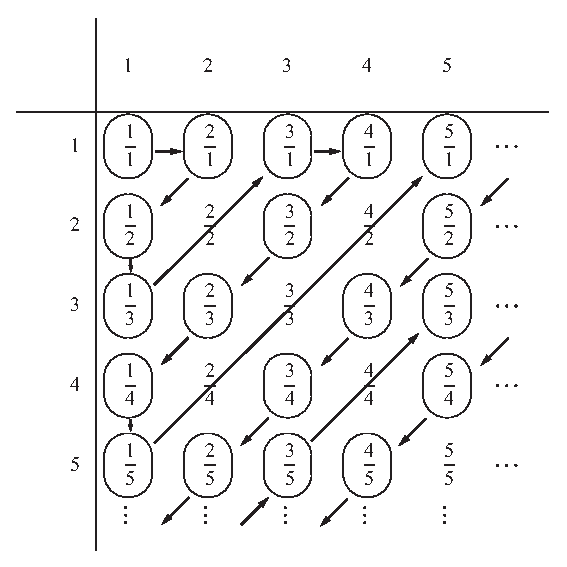
\includegraphics{figps-rationals.eps}
\caption{Counting the Positive Rational Numbers}\label{fig:positiverationals}
\end{center}
\end{figure}
The top row in Figure~\ref{fig:positiverationals} represents the numerator of the rational number, and the left column represents the denominator.  We follow the arrows in 
Figure~\ref{fig:positiverationals} to define $f\x \mathbb{N} \to \mathbb{Q}^+$.  The idea is to start in the upper left corner of the table and move to successive diagonals  as follows:
\begin{itemize}
\item We start with all fractions in which the sum of the numerator and denominator is 2 
$\left( \text{only } \dfrac{1}{1} \right)$.  So $f ( 1 ) = \dfrac{1}{1}$.

\item We next use those fractions in which the sum of the numerator and denominator is 3.  So 
$f ( 2 ) = \dfrac{2}{1}$ and $f ( 3 ) = \dfrac{1}{2}$.

\item We next use those fractions in which the sum of the numerator and denominator is 4.  So 
$f ( 4 ) = \dfrac{1}{3}$, $f ( 5 ) = \dfrac{3}{1}$.  We skipped 
$\dfrac{2}{2}$ since $\dfrac{2}{2} = \dfrac{1}{1}$.  In this way, we will ensure that the function $f$ is a one-to-one function.
\end{itemize}
We now continue with successive diagonals omitting fractions that are not in lowest terms.  This process guarantees that the function $f$ will be an injection and a surjection.  Therefore, 
$\mathbb{N} \approx \mathbb{Q}^+$ and $\text{card} ( \mathbb{Q}^+ ) = \aleph_0$.
\end{myproof}

\newpar
\note For another proof of Theorem~\ref{T:positiverationals}, see exercise~(\ref{A:Qcountable}) on page~\pageref{A:Qcountable}.

\newpar
Since $\mathbb{Q}^+$ is countable, it seems reasonable to expect that $Q$ is countable.  We will explore this soon.  On the other hand, at this point, it may also seem reasonable to ask, 
\begin{center}
``Are there any uncountable sets?''
\end{center}
The answer to this question is yes, but we will wait until the next section to prove that certain sets are uncountable.  We still have a few more issues to deal with concerning countable sets.
\endinput

\subsection*{Countably Infinite Sets}

\begin{theorem}\label{T:addonetocountable}
If $A$ is a countably infinite set, then $A \cup \left\{ x \right\}$ is a countably infinite set.
\end{theorem}
%
\begin{myproof}
Let $A$ be a  countably infinite set.  Then there exists a bijection $f\x \mathbb{N} \to A$.  Since $x$ is either in $A$ or not in $A$, we can consider two cases.

\newpar
If $x \in A$, then $A \cup \left\{ x \right\} = A$ and $A \cup \left\{ x \right\}$ is countably infinite.

\newpar
If $x \notin A$, define $g\x \mathbb{N} \to A \cup \left\{ x \right\}$ by
\begin{equation} \notag
g( n ) = 
\begin{cases}
x                        &\text{if $n = 1$} \\
f ( n - 1 )   &\text{if $n > 1$.}
\end{cases}
\end{equation}
The proof that the function $g$ is a bijection is Exercise~(\ref{exer:addonetocountable}).  Since $g$ is a bijection, we have proved that $A \cup \left\{ x \right\} \approx \N$ and hence, $A \cup \left\{ x \right\}$ is countably infinite.
\end{myproof}
%
\begin{theorem}\label{T:addfinitetocountable}
If $A$ is a countably infinite set and $B$ is a finite set, then $A \cup B$ is a countably infinite set.
\end{theorem}
%
\begin{myproof}
Exercise~(\ref{exer:addfinitetocountable}) on page~\pageref{exer:addfinitetocountable}.
\end{myproof}
%

Theorem~\ref{T:addfinitetocountable} says that if we add a finite number of elements to a countably infinite set, the resulting set is still countably infinite.  In other words, the cardinality of the new set is the same as the cardinality of the original set.  Finite sets behave very differently in the sense that if we add elements to a finite set, we will change the cardinality.  What may even be more surprising  is the result in Theorem~\ref{T:unionofcountable} that states that the union of two countably infinite (disjoint) sets is countably infinite.  The proof of this result is similar to the proof that the integers are countably infinite  (Theorem~\ref{T:ZequivtoN}).  In fact, if $A = \{a_1, a_2, a_3, \ldots \}$ and $B = \{b_1, b_2, b_3, \ldots \}$, then we can use the following diagram to help define a bijection from $\N$ to $A \cup B$.


\begin{figure}[h]
$$
\BeginTable
\BeginFormat
| c | c | c | c | c | c | c | c | c | c | c |
\EndFormat
" 1 " 2 " 3 " 4 " 5 " 6 " 7 " 8 " 9 " 10 " $\cdots$ " \\
" $\downarrow$ " $\downarrow$ " $\downarrow$ " $\downarrow$ " $\downarrow$ " $\downarrow$ " $\downarrow$ " $\downarrow$ " $\downarrow$ " $\downarrow$ " $\cdots$ "\\
" $a_1$ " $b_1$ " $a_2$ " $b_2$ " $a_3$ " $b_3$ " $a_4$ " $b_4$ " $a_5$ " $b_5$ "  $\cdots$ " \\
\EndTable
$$
\caption{A Function from $\N$ to $A \cup B$} \label{fig:functionNtoUnion}
\end{figure}


\begin{theorem}\label{T:unionofcountable}
If $A$ and $B$ are disjoint countably infinite sets,
\index{countably infinite sets!union of}%
 then $A \cup B$ is a countably infinite set.
\end{theorem}
%
\begin{myproof}
Let $A$ and $B$ be countably infinite sets and let $f\x \mathbb{N} \to A$ and 
$g\x \mathbb{N} \to B$ be bijections.  Define $h\x \mathbb{N} \to A \cup B$ by
\begin{equation} \notag
h( n ) = 
\begin{cases}
f \!\left( \dfrac{n+1}{2} \right)                        &\text{if $n$ is odd} \\
                                                       & \\
g \!\left( \dfrac{n}{2} \right)                          &\text{if $n$ is even}.
\end{cases}
\end{equation}
It is left as Exercise~(\ref{exer:unionofcountable}) on 
page~\pageref{exer:unionofcountable} to prove that the function $h$ is a bijection.
\end{myproof}

Since we can write the set of rational numbers $\Q$ as the union of the set of nonnegative rational numbers and the set of negative rational numbers, we can use the results in Theorem~\ref{T:positiverationals}, Theorem~\ref{T:addonetocountable}, and Theorem~\ref{T:unionofcountable} to prove the following theorem.

\begin{theorem}\label{T:Qiscountable}
The set $\mathbb{Q}$ of all rational numbers is countably infinite.
\end{theorem}
%
\begin{myproof}
Exercise~(\ref{exer:Qiscountable}) on page~\pageref{exer:Qiscountable}.
\end{myproof}
%\hbreak
%
\index{countably infinite sets!subsets of|(}%
In Section~\ref{S:finitesets}, we proved that any subset of a finite set is finite 
(Theorem~\ref{T:finitesubsets}).  A similar result should be expected for countable sets. We first prove that every subset of $\mathbb{N}$ is countable.  For an infinite subset $B$ of 
$\mathbb{N}$, the idea of the proof is to define a function $g\x  \mathbb{N} \to B$ by removing the elements from $B$ from smallest to the next smallest to the next smallest, and so on.  
We do this by defining the function $g$ recursively as follows:
\begin{itemize}
\item Let $g ( 1 )$ be the smallest natural number in $B$.
\item Remove $g ( 1 )$ from $B$ and let $g ( 2 )$ be the smallest natural number in \linebreak
$B - \left\{ g ( 1 ) \right\}$.
\item Remove $g ( 2 )$ and let $g ( 3 )$ be the smallest natural number in 
\linebreak
$B - \left\{ g ( 1 ), g ( 2 ) \right\}$.
\item We continue this process.  The formal recursive definition of $g\x  \mathbb{N} \to B$ is included in the proof of Theorem~\ref{T:subsetsofN}.
\end{itemize}
%
\begin{theorem}\label{T:subsetsofN}
Every subset of the natural numbers is countable.
\end{theorem}
%
\begin{myproof}
Let $B$ be a subset of $\mathbb{N}$.  If $B$ is finite, then $B$ is countable.  So we next assume that $B$ is infinite.  We will next give a recursive definition of a function 
$g\x  \mathbb{N} \to B$ and then prove that $g$ is a bijection.
\begin{itemize}
\item Let $g ( 1 )$ be the smallest natural number in $B$.
\item For each $n \in \mathbb{N}$, the set 
$B - \left\{ g ( 1 ), g ( 2 ), \ldots, g ( n ) \right\}$ is not empty since $B$ is infinite.  Define $g ( n + 1 )$ to be the smallest natural number in 
\linebreak
$B - \left\{ g ( 1 ), g ( 2 ), \ldots, g ( n ) \right\}$.
\end{itemize}
The proof that the function $g$ is a bijection is Exercise~(\ref{exer:subsetofN}) on page~\pageref{exer:subsetofN}.  
\end{myproof}
%
\begin{corollary}\label{C:subsetofcountable}
Every subset of a countable set is countable.
\end{corollary}
%
\begin{myproof}
Exercise~(\ref{exer:subsetofcountable}) on page~\pageref{exer:subsetofcountable}.
\end{myproof}
\index{countably infinite sets!subsets of|)}%

\hbreak

\endinput


\endinput



%\hrule
%

Since $\mathbb{Q}^+$ is countable, it seems reasonable to expect that $Q$ is countable.  We will explore this soon.  On the other hand, at this point, it may also seem reasonable to ask, 
\begin{center}
``Are there any uncountable sets?''
\end{center}

\begin{figure}[h]
\begin{center}
\setlength{\unitlength}{0.5cm}
\begin{picture}(20,20)
\put(4,18){1}
\put(7,18){2}
\put(10,18){3}
\put(13,18){4}
\put(16,18){5}

\put(2,15){1}
\put(2,12){2}
\put(2,9){3}
\put(2,6){4}
\put(2,3){5}

\put(0,16.5){\line(1,0){20}}
\put(3,0){\line(0,1){20}}

\put(4,15){$\dfrac{1}{1}$}
\put(7,15){$\dfrac{2}{1}$}
\put(10,15){$\dfrac{3}{1}$}
\put(13,15){$\dfrac{4}{1}$}
\put(16,15){$\dfrac{5}{1}$}
\put(18,15){$\cdots$}

\put(4.2,15.2){\oval(1.8,2.4)}
\put(7.2,15.2){\oval(1.8,2.4)}
\put(10.2,15.2){\oval(1.8,2.4)}
\put(13.2,15.2){\oval(1.8,2.4)}
\put(16.2,15.2){\oval(1.8,2.4)}

\put(4,12){$\dfrac{1}{2}$}
\put(7,12){$\dfrac{2}{2}$}
\put(10,12){$\dfrac{3}{2}$}
\put(13,12){$\dfrac{4}{2}$}
\put(16,12){$\dfrac{5}{2}$}
\put(18,12){$\cdots$}

\put(4.2,12.2){\oval(1.8,2.4)}
\put(10.2,12.2){\oval(1.8,2.4)}
\put(16.2,12.2){\oval(1.8,2.4)}

\put(4,9){$\dfrac{1}{3}$}
\put(7,9){$\dfrac{2}{3}$}
\put(10,9){$\dfrac{3}{3}$}
\put(13,9){$\dfrac{4}{3}$}
\put(16,9){$\dfrac{5}{3}$}
\put(18,9){$\cdots$}

\put(4.2,9.2){\oval(1.8,2.4)}
\put(7.2,9.2){\oval(1.8,2.4)}
\put(13.2,9.2){\oval(1.8,2.4)}
\put(16.2,9.2){\oval(1.8,2.4)}

\put(4,6){$\dfrac{1}{4}$}
\put(7,6){$\dfrac{2}{4}$}
\put(10,6){$\dfrac{3}{4}$}
\put(13,6){$\dfrac{4}{4}$}
\put(16,6){$\dfrac{5}{4}$}
\put(18,6){$\cdots$}

\put(4.2,6.2){\oval(1.8,2.4)}
\put(10.2,6.2){\oval(1.8,2.4)}
\put(16.2,6.2){\oval(1.8,2.4)}

\put(4,3){$\dfrac{1}{5}$}
\put(7,3){$\dfrac{2}{5}$}
\put(10,3){$\dfrac{3}{5}$}
\put(13,3){$\dfrac{4}{5}$}
\put(16,3){$\dfrac{5}{5}$}
\put(18,3){$\cdots$}

\put(4.2,3.2){\oval(1.8,2.4)}
\put(7.2,3.2){\oval(1.8,2.4)}
\put(10.2,3.2){\oval(1.8,2.4)}
\put(13.2,3.2){\oval(1.8,2.4)}

\put(4,1){$\vdots$}
\put(7,1){$\vdots$}
\put(10,1){$\vdots$}
\put(13,1){$\vdots$}
\put(16,1){$\vdots$}

\put(5.2,15){\vector(1,0){1}}

\put(6.5,14){\vector(-1,-1){1}}
\put(4.3,11){\vector(0,-1){.5}}

\put(5.2,10){\vector(1,1){4}}
\put(11.2,15){\vector(1,0){1}}
\put(12.5,14){\vector(-1,-1){1}}
\put(9.5,11){\vector(-1,-1){1}}
\put(6.5,8){\vector(-1,-1){1}}
\put(4.3,5){\vector(0,-1){.5}}
\put(5.2,4){\vector(1,1){10}}

\put(18.5,14){\vector(-1,-1){1}}
\put(15.5,11){\vector(-1,-1){1}}
\put(12.5,8){\vector(-1,-1){1}}
\put(9.5,5){\vector(-1,-1){1}}
\put(6.5,2){\vector(-1,-1){1}}

\put(8.5,1){\vector(1,1){1}}
\put(11.1,4.1){\vector(1,1){4}}

\put(18.5,8){\vector(-1,-1){1}}
\put(15.5,5){\vector(-1,-1){1}}
\put(12.5,2){\vector(-1,-1){1}}
\end{picture}
\caption{Counting the Positive Rational Numbers}\label{fig:positiverationals}
\end{center}
\end{figure}

\section*{Exercises \ref{S:infinitesets}}

\begin{enumerate}
\xitem State whether each of the following is true or false.
\label{exer:sec93-1}%
\begin{enumerate}
\item If a set $A$ is countably infinite, then $A$ is infinite.
\item If a set $A$ is countably infinite, then $A$ is countable.
\item If a set $A$ is uncountable, then $A$ is not countably infinite.
\item If $A \approx \mathbb{N}_k$ for some $k \in \mathbb{N}$, then $A$ is not countable.
\end{enumerate}

\item Prove that each of the following sets is countably infinite.
\label{exer:sec93-2}%
\begin{enumerate}
\item The set $F^+$ of all natural numbers that are multiples of 5
\item The set $F$ of all integers that are multiples of 5
\end{enumerate}
\begin{multicols}{2}
\begin{enumerate} \setcounter{enumii}{2}
\item $\left\{ \left. \dfrac{1}{2^k} \right| k \in \mathbb{N} \right\}$
\item $\left\{ n \in \mathbb{Z} \mid n \geq -10 \right\}$
\yitem $\mathbb{N} - \left\{ 4, 5, 6 \right\}$
\yitem $\left\{ m \in \mathbb{Z} \mid m \equiv 2 \pmod 3 \right\}$
\end{enumerate}
\end{multicols}

\item Prove part~(\ref{T:subsetisinfinite2}) of Theorem~\ref{T:subsetisinfinite}. 
\label{exer:subsetisinfinite}%

Let $A$ and $B$ be sets.  If $A$ is infinite and $A \subseteq B$, then $B$ is infinite.



\item Complete the proof of Theorem~\ref{T:addonetocountable} by proving the following:
\label{exer:addonetocountable}%

\noindent
Let $A$ be a countably infinite set and $x \notin A$.  If $f\x \mathbb{N} \to A$ is a bijection,  then $g$ is a bijection, where
$g\x \mathbb{N} \to A \cup \left\{ x \right\}$ by
\begin{equation} \notag
g( n ) = 
\begin{cases}
x                        &\text{if $n = 1$} \\
f ( n - 1 )   &\text{if $n > 1$}.
\end{cases}
\end{equation}

\xitem Prove Theorem~\ref{T:addfinitetocountable}. 
\label{exer:addfinitetocountable}%

If $A$ is a countably infinite set and $B$ is a finite set, then $A \cup B$ is a countably infinite set.

\hint  Let $\text{card} ( B ) = n$ and use a proof by induction on $n$.  
Theorem~\ref{T:addonetocountable} is the basis step.

\xitem Complete the proof of Theorem~\ref{T:unionofcountable} by proving the following: 
\label{exer:unionofcountable}%

Let $A$ and $B$ be disjoint countably infinite sets and let $f\x \mathbb{N} \to A$ and 
$g\x \mathbb{N} \to B$ be bijections.  Define $h\x \mathbb{N} \to A \cup B$ by
\begin{equation} \notag
h( n ) = 
\begin{cases}
f \!\left( \dfrac{n+1}{2} \right)                        &\text{if $n$ is odd} \\
                                                       & \\
g \!\left( \dfrac{n}{2} \right)                          &\text{if $n$ is even}.
\end{cases}
\end{equation}
Then the function $h$ is a bijection.

\xitem Prove Theorem~\ref{T:Qiscountable}.
\label{exer:Qiscountable}%

The set $\mathbb{Q}$ of all rational numbers is countable.

\hint  Use Theorem~\ref{T:addonetocountable} and Theorem~\ref{T:unionofcountable}.

\xitem Prove that if $A$ is countably infinite and $B$ is finite, then $A - B$ is countably infinite. 
\label{exer:countinf-finite}%

\item Define $f\x \mathbb{N} \times \mathbb{N} \to \mathbb{N}$ as follows:  For each 
$( m, n ) \in \mathbb{N} \times \mathbb{N}$, 
\label{exer:NxNbijection}%
\[
f ( m, n ) = 2^{m-1} (2n - 1 ).
\] 
\begin{enumerate}
\item Prove that $f$ is an injection.  \hint  If 
$f ( m, n ) = f ( s, t )$, there are three cases to consider:  $m > s$, $m < s$, and $m = s$. Use laws of exponents to prove that the first two cases lead to a contradiction.

\item Prove that $f$ is a surjection.  \hint  You may use the fact that if $y \in \mathbb{N}$, then $y = 2^k x$, where $x$ is an odd natural number and $k$ is a non-negative integer.  This is actually a consequence of the Fundamental Theorem of Arithmetic, Theorem~\ref{T:fundtheorem}.  [See Exercise~(\ref{exer:fundtheoremcons}) in Section~\ref{S:primefactorizations}.]

\item Prove that $\mathbb{N} \times \mathbb{N} \approx \mathbb{N}$ and hence that 
$\text{card} \left( \mathbb{N} \times \mathbb{N} \right) = \aleph_0$.
\end{enumerate}

\item Use Exercise~(\ref{exer:NxNbijection}) to prove that if $A$ and $B$ are countably infinite sets, then $A \times B$ is a countably infinite set.

\item Complete the proof of Theorem~\ref{T:subsetsofN} by proving that the function $g$ defined in the proof is a bijection from $\mathbb{N}$ to $B$. 
\label{exer:subsetofN}%

\hint  To prove that $g$ is an injection, it might be easier to prove that for all 
$r, s \in \mathbb{N}$, if $r \ne s$, then $g ( r ) \ne g ( s )$.  To do this, we may assume that $r < s$ since one of the two numbers must be less than the other.  Then notice that $g ( r ) \in \left\{ g( 1 ), g( 2 ), \ldots, g( s-1 ) \right\}$.

To prove that $g$ is a surjection, let $b \in B$ and notice that for some $k \in \mathbb{N}$, there will be $k$ natural numbers in $B$ that are less than $b$.

\item Prove Corollary~\ref{C:subsetofcountable}, which states that every subset of a countable set is countable. 
\label{exer:subsetofcountable}%

\hint  Let $S$ be a countable set and assume that $A \subseteq S$.  There are two cases:  $A$ is finite or $A$ is infinite.  If $A$ is infinite, let $f\x S \to \mathbb{N}$ be a bijection and define $g\x A \to f ( A )$ by $g ( x ) = f ( x )$, for each $x \in A$.

\item Use Corollary~\ref{C:subsetofcountable} to prove that the set of all rational numbers between 0 and 1 is countably infinite. 

\item \label{exer:tworationals} Let $a, b \in \mathbb{Q}$ with $a < b$. On page~\pageref{tworationals}, we proved that $c = \dfrac{a+b}{2}$ is a rational number and that $a < c < b$, which proves that here is a rational number between any two (unequal) rational numbers.
\begin{enumerate}
\item Now let  $c_1 = \dfrac{a+b}{2}$, and define $c_2 = \dfrac{c_1 + b}{2}$.  Prove that 
$c_1 < c_2 < b$ and hence, that $a < c_1 < c_2 < b$.


\item For each $k \in \mathbb{N}$, define
\[
c_{k+1} = \frac{c_k + b}{2}.
\]
Prove that for each $k \in \mathbb{N}$, $a < c_k < c_{k+1} < b$.  Use this to explain why the set 
$\left\{ c_k \mid k \in \mathbb{N} \right\}$ is an infinite set where each element is a rational number between $a$ and $b$.
\end{enumerate}
\end{enumerate}



\subsection*{Explorations and Activities}
\setcounter{oldenumi}{\theenumi}
\begin{enumerate} \setcounter{enumi}{\theoldenumi}
\item \textbf{Another Proof that $\mathbf{\Q^+}$ Is Countable}. \label{A:Qcountable} 
For this activity, it may be helpful to use the Fundamental Theorem of Arithmetic (see Theorem~\ref{T:fundtheorem} on page~\pageref{T:fundtheorem}).  Let $\Q^+$ be the set of positive rational numbers.  Every positive rational number has a unique representation as a fraction $\dfrac{m}{n}$, where $m$ and $n$ are relatively prime natural numbers.
We will now define a function $f\x  \Q^+ \to \N$ as follows:

\eighth
\noindent
If $x \in \Q^+$ and $x = \dfrac{m}{n}$, where $m, n \in \N$, $n \ne 1$ and $\gcd(m, n) = 1$, we write
\[
\begin{aligned}
m &= p_1^{\alpha_1} p_2^{\alpha_2} \cdots p_r^{\alpha_r}, \quad \text{and} \\
n &= q_1^{\beta_1} q_2^{\beta_2} \cdots q_s^{\beta_s}, 
\end{aligned}
\]
where $p_1$, $p_2$, \ldots, $p_r$ are distinct prime numbers, $q_1$, $q_2$, \ldots, $q_s$ are distinct prime numbers, and 
$\alpha_1$, $\alpha_2$, \ldots, $\alpha_r$ and $\beta_1$, $\beta_2$, \ldots, $\beta_s$ are natural numbers.    
%In addition, for each $j$ with $1 \leq j \leq r$ and for each $k$ with 
%$1 \leq k \leq s$, $p_j \ne q_k$.  
We also write $1 = 2^0$ when $m = 1$.  We then define

\[
f(x) = p_1^{2\alpha_1} p_2^{2\alpha_2} \cdots p_r^{2\alpha_r}
q_1^{2\beta_1 -1 } q_2^{2 \beta_2 - 1} \cdots q_s^{2 \beta_s - 1}.
\]

\noindent
If $x = \dfrac{m}{1}$, then we define 
$f(x) = p_1^{2\alpha_1} p_2^{2\alpha_2} \cdots p_r^{2\alpha_r} = m^2$.  

\begin{enumerate}
\item Determine $f \!\left( \dfrac{2}{3} \right)$, $f \!\left( \dfrac{5}{6} \right)$, 
$f ( 6 )$, $f ( \dfrac{12}{25} )$, 
$f \!\left( \dfrac{375}{392} \right)$, and $f \!\left( \dfrac{2^3 \cdot 11^3}{3 \cdot 5^4} \right)$.

\item If possible, find $x \in \Q^+$ such that $f(x) = 100$.

\item If possible, find $x \in \Q^+$ such that $f(x) = 12$.

\item If possible, find $x \in \Q^+$ such that $f(x) = 2^8 \cdot 3^5 \cdot 13 \cdot 17^2$.

\item Prove that the function $f$ is an injection.

\item Prove that the function $f$ is a surjection.

\item What has been proved?
\end{enumerate}
\end{enumerate}


\hbreak


\endinput





%
\section{Uncountable Sets}\label{S:uncountablesets}
%\markboth{Chapter~\ref{C:topicsinsets}. Topics in Set Theory}{\ref{S:uncountablesets}. 
%Uncountable Sets}
\setcounter{previewactivity}{0}
%
\begin{previewactivity}[\textbf{The Game of Dodge Ball}]\label{PA:dodgeball} \hfill \\
\index{Dodge Ball}%
(From \emph{The Heart of Mathematics: An Invitation to Effective Thinking} by Edward B. Burger and Michael Starbird, Key Publishing Company, \copyright 2000 by Edward B. Burger and Michael Starbird.)

Dodge Ball is a game for two players.  It is played on a game board such as the one shown in Figure~\ref{fig:dodgeball}.
\begin{figure}[h]
\begin{center}
\setlength{\unitlength}{0.5cm}
\begin{picture}(15,21)
\put(1,20){Player One's Array}
\put(1,19){\line(1,0){13}}
\put(1,17){\line(1,0){13}}
\put(1,15){\line(1,0){13}}
\put(1,13){\line(1,0){13}}
\put(1,11){\line(1,0){13}}
\put(1,9){\line(1,0){13}}
\put(1,7){\line(1,0){13}}

\put(1,7){\line(0,1){12}}
\put(2,7){\line(0,1){12}}
\put(4,7){\line(0,1){12}}
\put(6,7){\line(0,1){12}}
\put(8,7){\line(0,1){12}}
\put(10,7){\line(0,1){12}}
\put(12,7){\line(0,1){12}}
\put(14,7){\line(0,1){12}}

\put(1.3,17.5){1}
\put(1.3,15.5){2}
\put(1.3,13.5){3}
\put(1.3,11.5){4}
\put(1.3,9.5){5}
\put(1.3,7.5){6}

\put(1,5){Player Two's Row}
\put(2,4){\line(1,0){12}}
\put(2,3){\line(1,0){12}}
\put(2,1){\line(1,0){12}}

\put(2,1){\line(0,1){3}}
\put(4,1){\line(0,1){3}}
\put(6,1){\line(0,1){3}}
\put(8,1){\line(0,1){3}}
\put(10,1){\line(0,1){3}}
\put(12,1){\line(0,1){3}}
\put(14,1){\line(0,1){3}}

\put(2.8,3.3){1}
\put(4.8,3.3){2}
\put(6.8,3.3){3}
\put(8.8,3.3){4}
\put(10.8,3.3){5}
\put(12.8,3.3){6}

\put(0,21){\line(1,0){15}}
\put(0,0){\line(1,0){15}}
\put(0,0){\line(0,1){21}}
\put(15,0){\line(0,1){21}}
\end{picture}
\caption{Game Board for Dodge Ball}\label{fig:dodgeball}
\end{center}
\end{figure}
Player One has a 6 by 6 array to complete and Player Two has a 1 by 6 row to complete.  Each player has six turns as described next.
\begin{itemize}
\item Player One begins by filling in the first horizontal row of his or her table with a sequence of six X's and O's, one in each square in the first row.

\item Then Player Two places either an X or an O in the first box of his or her row.  At this point, Player One has completed the first row and Player Two has filled in the first box of his or her row with one letter.

\item The game continues with Player One completing a row with six letters (X's and O's), one in each box of the next row followed by Player Two writing one letter (an X or an O) in the next box of his or her row.  The game is completed when Player One has completed all six rows and Player Two has completed all six boxes in his or her row.
\end{itemize}

\newpar
\textbf{Winning the Game}
\begin{itemize}
\item Player One wins if any horizontal row in the 6 by 6 array is identical to the row that Player Two created.  (Player One matches Player Two.)

\item Player Two wins if Player Two's row of six letters is different than each of the six rows produced by Player One.  (Player Two ``dodges'' Player One.)
\end{itemize}
There is a winning strategy for one of the two players.  This means that there is plan by which one of the two players will always win.  Which player has a winning strategy?  Carefully describe this winning strategy.


\newpar
\textbf{Applying the Winning Strategy to Lists of Real Numbers} \\
Following is a list of real numbers between 0 and 1.  Each real number is written as a decimal number.
\begin{align*}
a_1 &= 0.1234567890   &  a_6 &= 0.0103492222 \\
a_2 &= 0.3216400000   &  a_7 &= 0.0011223344 \\
a_3 &= 0.4321593333   &  a_8 &= 0.7077700022 \\
a_4 &= 0.9120930092   &  a_9 &= 0.2100000000 \\
a_5 &= 0.0000234102   & a_{10} &= 0.9870008943 
\end{align*}
Use a method similar to the winning strategy in the game of Dodge Ball to write a real number (in decimal form) between 0 and 1 that is not in this list of 10 numbers.

\begin{enumerate}
  \item Do you think your method could be used for any list of 10 real numbers between 0 and 1 if the goal is to write a real number between 0 and 1 that is not in the list?
  \item Do you think this method could be extended to a list of 20 different real numbers?  To a list of 50 different real numbers?
  \item Do you think this method could be extended to a countably infinite list of real numbers?
\end{enumerate}

\end{previewactivity}
\hbreak

\endinput

\begin{previewactivity}[\textbf{Functions from a Set to Its Power Set}]\label{PA:powerset} \hfill \\
Let $A$ be a set.  In Section~\ref{S:setoperations}, we defined the \textbf{power set}
\index{power set}% 
$\mathcal{P} ( A )$ of $A$ to be the set of all subsets of $A$.  This means that
\begin{center}
$X \in \mathcal{P} ( A )$ if and only if $X \subseteq A$.
\end{center}
%
Theorem~\ref{T:powerset} in Section~\ref{S:setoperations} states that if a set $A$ has $n$ elements, then $A$ has $2^n$ subsets or that $\mathcal{P} ( A )$ has 
$2^n$ elements.  Using our current notation for cardinality, this means that
%
\begin{center}
if $\text{card} ( A ) = n$, then 
$\text{card} ( \mathcal{P} ( A ) ) = 2^n$.
\end{center}
%
(The proof of this theorem was Exercise~(\ref{exer:powerset}) on page~\pageref{exer:powerset}.)
%\begin{enumerate}
%\item Determine the power set of each of the following sets:
%\begin{multicols}{2}
%\begin{enumerate}
%\item $A = \left\{a, b \right\}$
%\item $B = \left\{a, b, c \right\}$
%\end{enumerate}
%\end{multicols}
%\end{enumerate}
%

We are now going to define and explore some functions from a set $A$ to its power set 
$\mathcal{P} ( A )$.  This means that the input of the function will be an element of $A$ and the output of the function will be a subset of $A$.

\begin{enumerate} 
\item Let $A = \left\{1, 2, 3, 4 \right\}$.  Define $f\x A \to \mathcal{P} ( A )$ by
%
\begin{multicols}{2}
$f ( 1 ) = \left\{ 1, 2, 3 \right\}$

$f ( 2 ) = \left\{ 1, 3, 4 \right\}$

$f ( 3 ) = \left\{ 1, 4 \right\}$

$f ( 4 ) = \left\{ 2, 4 \right\}$.
\end{multicols}
%
\begin{enumerate}
\item Is $1 \in f ( 1 )$?  Is $2 \in f ( 2 )$? Is 
$3 \in f ( 3 )$?  Is $4 \in f ( 4 )$?

\item Determine $S = \left\{ x \in A \mid x \notin f ( x ) \right\}$.

\item Notice that $S \in \mathcal{P} ( A )$.  Does there exist an element $t$ in $A$ such that $f ( t ) = S$?  That is, is $S \in \text{range} ( f )$?
 
\end{enumerate}

\item Let $A = \left\{1, 2, 3, 4 \right\}$.  Define $f\x A \to \mathcal{P} ( A )$ by 
%
\begin{center}
$f ( x ) = A - \left\{ x \right\}$ for each $x \in A$.
\end{center}
%
\begin{multicols}{2}
\begin{enumerate}
\item Determine $f ( 1 )$.  Is $1 \in f ( 1 )$?
\item Determine $f ( 2 )$.  Is $2 \in f ( 2 )$?
\item Determine $f ( 3 )$.  Is $3 \in f ( 3 )$?
\item Determine $f ( 4 )$.  Is $4 \in f ( 4 )$?
\end{enumerate}
\end{multicols}
%
\begin{enumerate} \setcounter{enumii}{4}
\item Determine $S = \left\{ x \in A \mid x \notin f ( x ) \right\}$.

\item Notice that $S \in \mathcal{P} ( A )$.  Does there exist an element $t$ in $A$ such that $f ( t ) = S$?  That is, is $S \in \text{range} ( f )$?
\end{enumerate}
%
\item Define $f\x \mathbb{N} \to \mathcal{P} ( \mathbb{N} )$ by
%
\begin{center}
$f ( n ) = \mathbb{N} - \left\{n^2, n^2-2n \right\}$, for each $n \in \mathbb{N}$.
\end{center}
%
\begin{enumerate}
\item Determine $f ( 1 )$, $f ( 2 )$, $f ( 3 )$, and 
$f ( 4 )$.  In each of these cases, determine if $k \in f ( k )$.
%
\item Prove that if $n > 3$, then $n \in f ( n )$.  \hint  Prove that if $n >3$, then 
$n^2 > n$ and $n^2 - 2n >n$.

\item Determine $S = \left\{ x \in \mathbb{N} \mid x \notin f ( x ) \right\}$.

\item Notice that $S \in \mathcal{P} ( \mathbb{N} )$.  Does there exist an element $t$ in $\mathbb{N}$ such that $f ( t ) = S$?  That is, is 
$S \in \text{range} ( f )$?

\end{enumerate}
\end{enumerate}
\end{previewactivity}
%\hbreak

\endinput



%
We have seen examples of sets that are countably infinite, but we have not yet seen an example of an infinite set that is uncountable.  We will do so in this section.  The first example of an uncountable set will be the open interval of real numbers $( 0, 1 )$.  The proof that this interval is uncountable uses a method similar to the winning strategy for Player Two in the game of Dodge Ball from \typeu Activity~\ref*{PA:dodgeball}.  Before considering the proof, we need to state an important result about decimal expressions for real numbers.

\subsection*{Decimal Expressions for Real Numbers}
\index{decimal expression!for a real number}%

In its decimal form, any real number $a$ in the interval $( 0, 1 )$ can be written as
$a = 0.a_1 a_2 a_3 a_4 \ldots ,$ where each $a_i$ is an integer with $0 \leq a_i \leq 9$.  For example,
\[
\frac{5}{12} = 0.416666 \ldots.
\]
We often abbreviate this as $\dfrac{5}{12} = 0.41 \overline{6}$ to indicate that the $6$ is repeated.  We can also repeat a block of digits.  For example, 
$\dfrac{5}{26} = 0.19 \overline{230769}$ to indicate that the block 230769 repeats.  That is, 
\[
\frac{5}{26} = 0.19230769230769230769 \ldots.
\]
There is only one situation in which a real number can be represented as a decimal in more than one way.  A decimal that ends with an infinite string of 9's is equal to one that ends with an infinite string of 0's.  For example, $0.3199999 \ldots$ represents the same real number as 
$0.3200000 \ldots .$  Geometric series can be used to prove that a decimal that ends with an infinite string of 9's is equal to one that ends with an infinite string of 0's, but we will not do so here.

\begin{defbox}{normalized}{A decimal representation of a real number $a$ is in \textbf{normalized form}
\index{decimal expression!normalized form}%
\index{normalized form!of a decimal expression}%
\label{normalizedform}%
 provided that there is no natural number $k$ such that for all natural numbers $n$ with $n > k$, $a_n = 9$.  That is, the decimal representation of $a$ is in normalized form if and only if it does not end with an infinite string of 9's.}
\end{defbox}

\newpar
One reason the normalized form is important is the following theorem (which will not be proved here).
\begin{theorem} \label{T:normalized} Two decimal numbers in normalized form are equal if and only if they have identical digits in each decimal position.
\end{theorem}

\endinput

\subsection*{Uncountable Subsets of $\boldsymbol{\mathbb{R}}$}
In the proof that follows, we will use only the normalized form for the decimal representation of a real number in the interval $( 0, 1 )$.
%\hbreak
%
\begin{theorem}\label{T:uncountableinterval}
The open interval $( 0, 1 )$ is an uncountable set.
\end{theorem}
%
\begin{myproof}
Since the interval $( 0, 1 )$ contains the infinite subset 
$\left\{\dfrac{1}{2}, \dfrac{1}{3}, \dfrac{1}{4}, \ldots \,\right\}$, we can use 
Theorem~\ref{T:subsetisinfinite}, to conclude that $( 0, 1 )$ is an infinite set.  So $( 0, 1 )$ is either countably infinite or uncountable.  We will prove that $( 0, 1 )$ is uncountable by proving that any function from $\N$ to $(0, 1)$ is not a surjection, and hence, there is no bijection from $\N$ to  $(0, 1)$.

So suppose that $f\x \mathbb{N} \to ( 0, 1 )$ is a function.  We will show that $f$ is not a surjection by showing that there exists an element in 
$( 0, 1 )$ that cannot be in the range of $f$.  Writing the images of the elements of 
$\mathbb{N}$ in normalized form, we can write
\[
\begin{aligned}
f ( 1 ) &= 0.a_{1 1} a_{1 2} a_{1 3} a_{1 4} a_{1 5} \ldots \\
f ( 2 ) &= 0.a_{2 1} a_{2 2} a_{2 3} a_{2 4} a_{2 5} \ldots \\
f ( 3 ) &= 0.a_{3 1} a_{3 2} a_{3 3} a_{3 4} a_{3 5} \ldots \\
f ( 4 ) &= 0.a_{4 1} a_{4 2} a_{4 3} a_{4 4} a_{4 5} \ldots \\
f ( 5 ) &= 0.a_{5 1} a_{5 2} a_{5 3} a_{5 4} a_{5 5} \ldots \\
                   & \vdots \\
f ( n ) &= 0.a_{n 1} a_{n 2} a_{n 3} a_{n 4} a_{n 5} \ldots \\
                   & \vdots \\
\end{aligned}
\]
Notice the use of the double subscripts. The number $a_{i j}$ is the $j^\text{th}$ digit to the right of the decimal point in the normalized decimal representation of $f ( i )$.

We will now construct a real number $b = 0.b_1 b_2 b_3 b_4 b_5 \ldots$ in $( 0, 1 )$ and in normalized form that is not in this list.  

\vskip6pt
\noindent
%\emph{Informal Side Note}:  
\note The idea is to start in the upper left corner and move down the diagonal in a manner similar to the winning strategy for Player Two in the game in 
\typeu Activity~\ref*{PA:dodgeball}.  At each step, we choose a digit that is not equal to the diagonal digit.
\vskip6pt

Start with $a_{1 1}$ in $f ( 1 )$.  We want to choose $b_1$ so that $b_1 \ne 0$, 
$b_1 \ne a_{1 1}$, and $b_1 \ne 9$. (To ensure that we end up with a decimal that is in normalized form, we make sure that each digit is not equal to 9.)  We then repeat this process with $a_{2 2}$, $a_{3 3}$, 
$a_{4 4}$, $a_{5 5}$, and so on.  So we let $b$ be the real number 
$b = 0.b_1 b_2 b_3 b_4 b_5 \ldots ,$ where for each $k \in \mathbb{N}$
\begin{equation} \notag
b_k = 
\begin{cases}
3         &\text{if $a_{k k} \ne 3$} \\
5         &\text{if $a_{k k} = 3$.}
\end{cases}
\end{equation}

\noindent
(The choice of 3 and 5 is arbitrary.  Other choices of distinct digits will also work.)

Now for each $n \in \mathbb{N}$, $b \ne f ( n )$ since $b$ and $f ( n )$ are in normalized form and $b$ and $f ( n )$ differ in the $n${th} decimal place.  Therefore, $f$ is not a surjection.  This proves that any function from $\mathbb{N}$ to $( 0, 1 )$ is not a surjection and hence, there is no bijection from $\mathbb{N}$ to $( 0, 1 )$.  Therefore, 
$( 0, 1 )$ is not countably infinite and hence must be an uncountable set.
\end{myproof}
\hbreak
%
\begin{prog} [\textbf{Dodge Ball and Cantor's Diagonal Argument}]\label{prog:diagonal} \hfill \\
The proof of Theorem~\ref{T:uncountableinterval} is often referred to as \textbf{Cantor's diagonal argument}.
\index{Cantor's diagonal argument}%
  It is named after the mathematician Georg Cantor, who first published the proof in 1874.  Explain the connection between the winning strategy for Player Two in Dodge Ball
\index{Dodge Ball}%
 (see \typeu Activity~\ref*{PA:dodgeball})  and the proof of Theorem~\ref{T:uncountableinterval} using Cantor's diagonal argument.
\end{prog}
\hbreak
%
The open interval $( 0, 1 )$ is our first example of an uncountable set.  The cardinal number of $( 0, 1 )$ is defined to be $\boldsymbol{c}$, 
\label{sym:continuum}% 
which stands for 
\textbf{the cardinal number of the continuum}.
\index{continuum}%
  So the two infinite cardinal numbers we have seen are $\aleph_0$ for countably infinite sets and $\boldsymbol{c}$.

\begin{defbox}{cardinalityc}{A set $A$ is said to have \textbf{cardinality}
\index{cardinality}%
\index{cardinality!$\boldsymbol{c}$}%
%\index{$\boldsymbol{c}$}%
  $\boldsymbol{c}$ provided that $A$ is equivalent to $( 0, 1 )$.  In this case, we write 
$\text{card} ( A ) = \boldsymbol{c}$ and say that the cardinal number of $A$ is 
$\boldsymbol{c}$.}
\end{defbox}

\noindent
The proof of Theorem~\ref{T:openintervals} is included in Progress Check~\ref{prog:openintervals}.

\begin{theorem}\label{T:openintervals}
Let $a$ and $b$ be real numbers with $a < b$.  The open interval $( a, b )$ is uncountable and has cardinality $\boldsymbol{c}$.
\end{theorem}
%
\begin{prog}[\textbf{Proof of Theorem~\ref{T:openintervals}}]\label{prog:openintervals} \hfill
\begin{enumerate}
\item In Part~(\ref{A:equivsets4}) of Progress Check~\ref{prog:equivsets}, we proved that if 
$b \in \R$ and $b > 0$, then the open interval $( 0, 1 )$ is equivalent to the open interval $( 0, b )$.  Now let $a$ and $b$ be real numbers with $a < b$.  Find a function 
\[
f\x  ( 0, 1 ) \to ( a, b )
\]
that is a bijection and conclude that the open interval $( 0, 1) \approx ( a, b )$.

\hint Find a linear function that passes through the points $( 0, a )$ and 
$( 1, b )$.  Use this to define the function $f$.  Make sure you prove that this function $f$ is a bijection.

\item Let $a, b, c, d$ be real numbers with $a < b$ and $c < d$.  Prove that the open interaval $( a, b )$ is equivalent to the open interval $( c, d )$.
\end{enumerate}
\end{prog}
\hbreak
%
\begin{theorem}\label{T:realsuncount}
The set of real numbers $\mathbb{R}$ is uncountable and has cardinality $\boldsymbol{c}$.
\end{theorem}
%
\begin{myproof}
Let $f\x  \left( -\dfrac{\pi}{2}, \dfrac{\pi}{2} \right) \to \mathbb{R}$ be defined by 
$f ( x ) = \tan x$, for each $x \in \mathbb{R}$.  The function $f$ is a bijection and, hence, 
$\left(-\dfrac{\pi}{2}, \dfrac{\pi}{2} \right) \approx \mathbb{R}$.  So by 
Theorem~\ref{T:openintervals}, $\mathbb{R}$ is uncountable and has cardinality $\boldsymbol{c}$.
\end{myproof}

\endinput

\subsection*{Cantor's Theorem}
\index{Cantor's Theorem}

We have now seen two different infinite cardinal numbers, $\aleph_0$ and $\boldsymbol{c}$.  It can seem surprising that there is more than one infinite cardinal number.  A reasonable question at this point is, ``Are there any other infinite cardinal numbers?''  The astonishing answer is that there are, and in fact, there are infinitely many different infinite cardinal numbers.  The basis for this fact is the following theorem, which states that a set is not equivalent to its power set.  The proof is  due to Georg Cantor (1845--1918),
\index{Cantor, Georg}%
and the idea for this proof was explored in \typeu Activity~\ref*{PA:powerset}. The basic idea of the proof is to prove that any function from a set $A$ to its power set cannot be a surjection.

\begin{theorem}[\textbf{Cantor's Theorem}]\label{T:cantor}
For every set $A$, $A$ and $\mathcal{P} ( A )$ do not have the same cardinality.
\end{theorem}
%
\begin{myproof}
Let $A$ be a set.  If $A = \emptyset$, then 
$\mathcal{P} ( A ) = \left\{ \emptyset \right\}$, which has cardinality 1.  Therefore, 
$\emptyset$ and $\mathcal{P} ( \emptyset )$ do not have the same cardinality.

Now suppose that $A \ne \emptyset$, and let $f\x  A \to \mathcal{P} ( A )$.  We will show that $f$ cannot be a surjection, and hence there is no bijection from $A$ to 
$\mathcal{P} ( A )$.  This will prove that $A$ is not equivalent to 
$\mathcal{P} ( A )$.  Define
\[
S = \left\{ x \in A \mid x \notin f ( x ) \right\}.
\]
Assume that there exists a $t$ in $A$ such that $f ( t ) = S$.  Now, either $t \in S$ or $t \notin S$.

\begin{itemize}
\item If $t \in S$, then $t \in \left\{ x \in A \mid x \notin f ( x ) \right\}$.  By the definition of $S$, this means that $t \notin f ( t )$.  However, 
$f ( t ) = S$ and so we conclude that $t \notin S$.  But now we have $t \in S$ and $t \notin S$.  This is a contradiction.

\item If $t \notin S$, then $t \notin \left\{ x \in A \mid x \notin f ( x ) \right\}$.  By the definition of $S$, this means that $t \in f ( t )$.  However, 
$f ( t ) = S$ and so we conclude that $t \in S$.  But now we have $t \notin S$ and $t \in S$.  This is a contradiction.
\end{itemize}
So in both cases we have arrived at a contradiction.  This means that there does not exist a 
$t$ in $A$ such that $f ( t ) = S$.  Therefore, any function from $A$ to 
$\mathcal{P} ( A )$ is not a surjection and hence not a bijection.  Hence, $A$ and 
$\mathcal{P} ( A )$ do not have the same cardinality. 
\end{myproof}
%\hbreak
%
\begin{corollary}\label{C:cantor}
$\mathcal{P} ( \mathbb{N} )$ is an infinite set that is not countably infinite.
\end{corollary}
%
\begin{myproof}
Since $\mathcal{P} ( \mathbb{N} )$ contains the infinite subset 
$\left\{ \left\{ 1 \right\}, \left\{ 2 \right\}, \left\{ 3 \right\} \ldots \,\right\}$, we can use 
Theorem~\ref{T:subsetisinfinite}, to conclude that $\mathcal{P} ( \mathbb{N} )$ is an infinite set.  By Cantor's Theorem (Theorem~\ref{T:cantor}), $\mathbb{N}$ and 
$\mathcal{P} ( \mathbb{N} )$ do not have the same cardinality.  Therefore, 
$\mathcal{P} ( \mathbb{N} )$ is not countable and hence is an uncountable set.
\end{myproof}
%
\subsection*{Some Final Comments about Uncountable Sets}
\begin{enumerate}
\item We have now seen that any open interval of real numbers is uncountable and has cardinality \
$\boldsymbol{c}$.  In addition, $\mathbb{R}$ is uncountable and has cardinality $\boldsymbol{c}$.  Now, Corollary~\ref{C:cantor} tells us that $\mathcal{P} ( \mathbb{N} )$ is uncountable.  A question that can be asked is, 
\begin{center}
``Does $\mathcal{P} ( \mathbb{N} )$ have the same cardinality as $\mathbb{R}$?''
\end{center}
The answer is yes, although we are not in a position to prove it yet.  A proof of this fact uses the following theorem, which is known as the Cantor-Schr\"{o}der-Bernstein Theorem.
\label{sec94:comment1}%
\end{enumerate}

\begin{theorem}[\textbf{Cantor-Schr\"{o}der-Bernstein}]\label{T:bernstein}
Let $A$ and $B$ be sets.  If there exist injections $f\x A \to B$ and $g\x B \to A$, then 
$A \approx B$.
\end{theorem}
\index{Cantor-Schr\"{o}der-Bernstein Theorem}%


In the statement of this theorem, notice that it is not required that the function $g$ be the inverse of the function $f$.  We will not prove the Cantor-Schr\"{o}der-Bernstein Theorem here.  
The following items will show some uses of this important theorem. 
%but a proof is given in Section~\ref{S:CSBproof}.  
%The following item will indicate another use of this theorem.

\begin{enumerate} \setcounter{enumi}{1}
\item The Cantor-Schr\"{o}der-Bernstein Theorem can also be used to prove that the closed interval 
$[ 0, 1 ]$ is equivalent to the open interval $( 0, 1 )$.  
See Exercise~(\ref{exer:closedinterval}) on page~\pageref{exer:closedinterval}.

\item Another question that was posed earlier is,
\begin{center}
``Are there other infinite cardinal numbers other than $\aleph_0$ and $\boldsymbol{c}$?''
\end{center}
Again, the answer is yes, and the basis for this is Cantor's Theorem (Theorem~\ref{T:cantor}).
We can start with $\text{card} ( \mathbb{N} ) = \aleph_0$.  We then define the following infinite cardinal numbers:
\begin{multicols}{2}
\begin{list}{}
\item $\text{card} ( \mathcal{P} ( \mathbb{N} ) ) = \alpha_1$.

\item $\text{card} ( \mathcal{P} ( \mathcal{P} ( \mathbb{N} ) ) ) = \alpha_2$.

\item $\text{card} ( \mathcal{P} ( \mathcal{P} ( \mathcal{P} ( \mathbb{N} ) ) ) ) = \alpha_3$. 
\label{sec94:comment3}%
\item $\vdots$
\end{list}
\end{multicols}

%\begin{multicols}{2}
%\begin{list}{}
%\item $\text{card} ( \mathcal{P} ( \mathbb{N} ) )$.
%
%\item $\text{card} ( \mathcal{P} ( \mathcal{P} ( \mathbb{N} ) ) )$.
%
%\item $\text{card} ( \mathcal{P} ( \mathcal{P} ( \mathcal{P} ( \mathbb{N} ) ) ) )$. 
%\label{sec94:comment3}%
%
%\item $\vdots$
%\end{list}
%\end{multicols}
Cantor's Theorem tells us that these are all different cardinal numbers, and so we are just using the lowercase Greek letter $\alpha$ (alpha) to help give names to these cardinal numbers.  In fact, although we will not define it here, there is a way to ``order'' these cardinal numbers in such a way that 
%\[
%\aleph_0 < \text{card} ( \mathcal{P} ( \mathbb{N} ) ) < \text{card} ( \mathcal{P} ( \mathcal{P} ( \mathbb{N} ) ) ) < \aleph_3 < \cdots.
%\]
\[
\aleph_0 < \alpha_1 < \alpha_2 < \alpha_3 < \cdots.
\]
Keep in mind, however, that even though these are different cardinal numbers, Cantor's Theorem does not tell us that these are the only cardinal numbers.

\item In Comment~(\ref{sec94:comment1}), we indicated that 
$\mathcal{P} ( \mathbb{N} )$ and $\mathbb{R}$ have the same cardinality.  Combining this with the notation in Comment~(\ref{sec94:comment3}), this means that 
\[
\alpha_1 = \boldsymbol{c}.
\]
However, this does not necessarily mean that $\boldsymbol{c}$ is the ``next largest'' cardinal number after 
$\aleph_0$.  A reasonable question is, ``Is there an infinite set with cardinality between 
$\aleph_0$ and $\boldsymbol{c}$?''  Rewording this in terms of the real number line, the question is, ``On the real number line, is there an infinite set of points that is not equivalent to the entire line and also not equivalent to the set of natural numbers?''  This question was asked by Cantor, but he was unable to find any such set.  He conjectured that no such set exists.  That is, he conjectured that $\boldsymbol{c}$ is really the next cardinal number after 
$\aleph_0$.  This conjecture has come to be known as the \textbf{Continuum Hypothesis}.
\index{Continuum Hypothesis}%
Stated somewhat more formally, the Continuum Hypothesis is
\begin{center}
There is no set $X$ such that $\aleph_0 < \text{card} ( X ) < \boldsymbol{c}$.
\end{center}
The question of whether the Continuum Hypothesis is true or false is one of the most famous problems in modern mathematics.  

Through the combined work of Kurt G\"{o}del
\index{G\"{o}del, Kurt}%
 in the 1930s and Paul Cohen
\index{Cohen, Paul}%
 in 1963, it has been proved that the Continuum Hypothesis cannot be proved or disproved from the standard axioms of set theory.  This means that either the Continuum Hypothesis or its negation can be added to the standard axioms of set theory without creating a contradiction.

\end{enumerate}
\hbreak 


\endinput



%\vskip6pt

%
%




\endinput

%\newpage
\section*{Exercises \ref{S:uncountablesets}}

\begin{enumerate}
\item Use an appropriate bijection to prove that each of the following sets has cardinality $\boldsymbol{c}$. 
\label{exer:sec94-1}%
\begin{multicols}{2}
\begin{enumerate}
\yitem $( 0, \infty )$
\yitem $( a, \infty )$, for any $a \in \mathbb{R}$
\item $\mathbb{R} - \left\{ 0 \right\}$
\item $\mathbb{R} - \left\{ a \right\}$, for any $a \in \mathbb{R}$
\end{enumerate}
\end{multicols}

\xitem Is the set of irrational numbers countable or uncountable? Prove that your answer is correct. 
\label{exer:irrationaluncount}%

\xitem Prove that if $A$ is uncountable and $A \subseteq B$, then $B$ is uncountable.
\label{exer:supersetofuncount}%

\xitem Do two uncountable sets always have the same cardinality?  Justify your conclusion. \label{exer93:uncountablesets}


\item Let  $C$  be the set of all infinite sequences, each of whose entries is the digit 0 or the digit 1.  For example,
\[
\begin{aligned}
\left( 1, 0, 1, 0, 1, 0, 1, 0, \ldots \right) &\in C; \\
\left( 0, 1, 0, 1, 1, 0, 1, 1, 1, 0, 1, 1, 1, 1, \ldots \right) &\in C; \\
\left( 2, 1, 0, 1, 1, 0, 1, 1, 1, 0, 1, 1, 1, 1, \ldots \right) &\notin C.
\end{aligned}
\]
Is the set  $C$  a countable set or an uncountable set?  Justify your conclusion.


\item The goal of this exercise is to use the Cantor-Schr\"{o}der-Bernstein Theorem to prove that the cardinality of the closed interval $[ 0, 1 ]$ is $\boldsymbol{c}$.
\label{exer:closedinterval}%

\begin{enumerate}
\item Find an injection $f\x  ( 0, 1 ) \to [ 0, 1 ]$.

\item Find an injection $h\x  [ 0, 1 ] \to ( -1, 2 )$.

\item Use the fact that $( -1, 2 ) \approx ( 0, 1 )$ to prove that there exists an injection 
$g\x  [ 0, 1 ] \to ( 0, 1 )$.  (It is only necessary to prove that the injection $g$ exists.  It is not necessary to determine a specific formula for 
$g ( x )$.)  

\note  Instead of doing Part~(b) as stated, another approach is to find an injection 
$k \x [0, 1] \to (0, 1)$.  Then, it is possible to skip Part~(c) and go directly to Part~(d).

\item Use the Cantor-Schr\"{o}der-Bernstein Theorem to conclude that \linebreak
$[ 0, 1 ] \approx ( 0, 1 )$ and hence that the cardinality of 
$[ 0, 1 ]$ is $\boldsymbol{c}$.
\end{enumerate}

\item In Exercise~(\ref{exer:closedinterval}), we proved that the closed interval $[ 0, 1 ]$ is uncountable and has cardinality $\boldsymbol{c}$.  Now let $a, b \in \mathbb{R}$ with $a < b$.  Prove that 
$[ a, b ] \approx [ 0, 1 ]$ and hence that $[ a, b ]$ is uncountable and has cardinality $\boldsymbol{c}$.



\item Is the set of all finite subsets of $\N$ countable or uncountable? Let $F$ be the set of all finite subsets of $\N$.  Determine the cardinality of the set $F$.

\eighth
\noindent
Consider defining a function $f:F \to \N$ that produces the following.
\begin{itemize}
  \item If $A = \{1, 2, 6 \}$, then $f(A) = 2^1 3^2 5^6$.
  \item If $B = \{3, 6 \}$, then $f(B) = 2^3 3^6$.
  \item If $C = \left\{ m_1, m_2, m_3, m_4 \right\}$ with $m_1 < m_2 < m_3 < m_4$, then 
           $f(C) = 2^{m_1} 3^{m_2} 5^{m_3} 7^{m_4}$.
\end{itemize}
It might be helpful to use the Fundamental Theorem of Arithmetic on page~\pageref{T:fundtheorem} and to denote the set of all primes as  $P = \left\{ p_1, p_2, p_3, p_4, \ldots \right\}$ with $p_1 < p_2 < p_3 < p_4 \cdots$.  Using the sets $A$, $B$, and $C$ defined above, we would then write
\[
f(A) = p_1^1 p_2^2 p_3^6, \quad f(B) = p_1^3 p_2^6, \quad \text{and} \quad f(C) = p_1^{m_1} p_2^{m_2} p_3^{m_3} p_4^{m_4}.
\]

\item In Exercise~(\ref{exer:irrationaluncount}), we showed that the set of irrational numbers is uncountable.  However, we still do not know the cardinality of the set of irrational numbers.  Notice that we can use $\Q^c$ to stand for the set of irrational numbers.

\begin{enumerate}
\item Construct a function $f\x \Q^c \to \R$ that is an injection.
\end{enumerate}
We know that any real number $a$ can be represented in decimal form as follows:
\[
a = A.a_1 a_2 a_3 a_4 \cdots a_n \cdots ,
\]
where $A$ is an integer and the decimal part $( 0.a_1 a_2 a_3 a_4 \cdots )$ is in normalized form.  (See page~\pageref{normalizedform}.)  We also know that the real number $a$ is an irrational number if and only $a$ has an infinite non-repeating decimal expansion.  We now associate with $a$ the real number
\setcounter{equation}{0}
\begin{equation}\label{exer:irrationalsuncount}
A.a_1 0 a_2 1 1 a_3 0 0 0 a_4 1 1 1 1 a_5 0 0 0 0 0 a_6 1 1 1 1 1 1 \cdots .
\end{equation}
Notice that to construct the real number in (\ref{exer:irrationalsuncount}), we started with the decimal expansion of $a$, inserted a 0 to the right of the first digit after the decimal point, inserted two 1's to the right of the second digit to the right of the decimal point, inserted three 0's to the right of the third digit to the right of the decimal point, and so on.

\begin{enumerate} \setcounter{enumii}{1}
\item Explain why the real number in (\ref{exer:irrationalsuncount}) is an irrational number.
\item Use these ideas to construct a function $g\x \R \to \Q^c$ that is an injection.
\item What can we now conclude by using the Cantor-Schr\"{o}der-Bernstein Theorem?
\end{enumerate}

\item Let $J$ be the unit open interval.  That is, $J = \left\{ x \in \R \mid 0 < x < 1 \right\}$ and let $S = \left\{ (x, y) \in \R \times \R \mid 0 < x < 1 \text{ and } 0 < y < 1 \right\}$.  We call $S$ the unit open square.  We will now define a function $f$ from $S$ to $J$.  Let 
$(a, b) \in S$ and write the decimal expansions of $a$ and $b$ in normalized form as
\begin{align*}
a &= 0.a_1 a_2 a_3 a_4 \cdots a_n \cdots \\
b &= 0.b_1 b_2 b_3 b_4 \cdots b_n \cdots .
\end{align*}
We then define $f(a, b) = 0.a_1 b_1 a_2 b_2 a_3 b_3 a_4 b_4 \cdots a_n b_n \cdots$.
\begin{enumerate}
\item Determine the values of $f ( 0.3, 0.625 )$, $f \!\left( \dfrac{1}{3}, \dfrac{1}{4} \right)$, and $f \!\left( \dfrac{1}{6}, \dfrac{5}{6} \right)$.

\item If possible, find $(x, y) \in S$ such that $f ( x, y ) = 0.2345$.

\item If possible, find $(x, y) \in S$ such that $f ( x, y ) = \dfrac{1}{3}$.

\item If possible, find $(x, y) \in S$ such that $f ( x, y ) = \dfrac{1}{2}$.

\item Explain why the function $f\x S \to J$ is an injection but is not a surjection.

\item Use the Cantor-Schr\"{o}der-Bernstein Theorem to prove that the cardinality of the unit open square $S$ is equal to $\boldsymbol{c}$. If this result seems surprising, you are in good company.  In a letter written in 1877 to the mathematician Richard Dedekind describing this result that he had discovered, Georg Cantor wrote, ``I see it but I do not believe it.''
\end{enumerate}
 
\end{enumerate}

\subsection*{Explorations and Activities}
\setcounter{oldenumi}{\theenumi}
\begin{enumerate} \setcounter{enumi}{\theoldenumi}
\item \textbf{The Closed Interval $\boldsymbol{ [ 0, 1 ]}$}.  \label{A:closedinterval}  In Exercise~(\ref{exer:closedinterval}), the Cantor-Schr\"{o}der-Bernstein Theorem was used to prove that the closed interval $[0, 1]$ has cardinality $\boldsymbol{c}$.  
%We have seen that $\text{card} \!\left( ( 0, 1 ) \right) = \boldsymbol{c}$ and 
%$\text{card} ( \mathbb{R} ) = \boldsymbol{c}$.  It would seem reasonable to expect that if we add the endpoints to the open interval $( 0, 1 )$, we would not change the cardinality.  That is, it might be reasonable to expect that 
%$\text{card} \!\left( [ 0, 1 ] \right) = \boldsymbol{c}$.  We have, in fact, indicated that the Cantor-Schr\"{o}der-Bernstein Theorem (Theorem~\ref{T:bernstein}) can be used to prove that this is true.  
This may seem a bit unsatisfactory since we have not proved the 
Cantor-Schr\"{o}der-Bernstein Theorem.  In this activity, we will prove that 
$\text{card} \!\left( [ 0, 1 ] \right) = \boldsymbol{c}$ by using appropriate bijections.

\begin{enumerate}
\item Let $f\x  [ 0, 1 ] \to [ 0, 1 )$ by
\begin{equation} \notag
f ( x ) = 
\begin{cases}
\dfrac{1}{n+1}         &\text{if $x=\dfrac{1}{n}$ for some $n \in \mathbb{N}$} \\
 %                     &                      \\
x        &\text{otherwise}.
\end{cases}
\end{equation}
\label{A:closedinterval1}%
%
\begin{enumerate}
\item Determine $f ( 0 )$, $f ( 1 )$, $f \!\left( \dfrac{1}{2} \right)$, 
$f \!\left( \dfrac{1}{3} \right)$, $f \!\left( \dfrac{1}{4} \right)$, and 
$f \!\left( \dfrac{1}{5} \right)$. 
\label{A:closedinterval1a}%
\item Sketch a graph of the function $f$.  \hint  Start with the graph of $y = x$ for 
$0 \leq x \leq 1$.  Remove the point $( 1, 1 )$ and replace it with the point 
$\!\left( 1, \dfrac{1}{2} \right)$.  Next, remove the point 
$\!\left( \dfrac{1}{2}, \dfrac{1}{2} \right)$ and replace it with the point 
$\!\left( \dfrac{1}{2}, \dfrac{1}{3} \right)$.  Continue this process of removing points on the graph of $y = x$ and replacing them with the points determined from the information in 
Part~(\ref{A:closedinterval1a}).  Stop after repeating this four or five times so that pattern of this process becomes apparent.

\item Explain why the function $f$ is a bijection.
\item Prove that $[ 0, 1 ] \approx [ 0, 1 )$.
\end{enumerate}
%
\item Let $g\x  [ 0, 1 ) \to ( 0, 1 )$ by
\begin{equation} \notag
g ( x ) = 
\begin{cases}
\dfrac{1}{2}           &\text{if $x=0$} \\
%                      &                      \\
\dfrac{1}{n+1}         &\text{if $x=\dfrac{1}{n}$ for some $n \in \mathbb{N}$} \\
%                      &                      \\
x        &\text{otherwise}.
\end{cases}
\end{equation}
\begin{enumerate}
\item Follow the procedure suggested in Part~(\ref{A:closedinterval1}) to sketch a graph of $g$.
\item Explain why the function $g$ is a bijection.
\item Prove that $[ 0, 1 ) \approx ( 0, 1 )$.
\end{enumerate}

\item Prove that $[ 0, 1 ]$ and $[ 0, 1 )$ are both uncountable and have cardinality $\boldsymbol{c}$.
\end{enumerate}
\end{enumerate}

\hbreak
\endinput

%
%\input{section94}
%\input{exercise94}

%\input{section95}

%\input{check-ch9}
%\newpage
\section{Chapter \ref{C:topicsinsets} Summary}

\subsection*{Important Definitions}
\begin{multicols}{2}
\begin{itemize}
\item Equivalent sets, page~\pageref*{equivsets}
\item Sets with the same cardinality, page~\pageref*{equivsets}
\item Finite set, page~\pageref*{cardinalityfinite}
\item Infinite set, page~\pageref*{cardinalityfinite}
\item Cardinality of a finite set, page~\pageref*{cardinalityfinite}
\item Cardinality of $\N$, page~\pageref*{aleph0}
\item $\aleph_0$, page~\pageref*{aleph0}
\item Countably infinite set, page~\pageref*{countinfinite}
\item Denumerable set, page~\pageref*{countinfinite}
\item Uncountable set, page~\pageref*{countinfinite}
\end{itemize}
\end{multicols}
\hbreak



\subsection*{Important Theorems and Results about Finite and Infinite Sets} 
\begin{itemize}
\item \textbf{Theorem~\ref{T:equivfinitesets}}.
\emph{Any set equivalent to a finite nonempty set $A$ is a finite set and has the same cardinality as $A$.}

\item \textbf{Theorem~\ref{T:finitesubsets}}.  
\emph{If $S$ is a finite set and $A$ is a subset of $S$, then $A$ is finite and 
$\text{card} ( A ) \leq \text{card} ( S )$.}

\item \textbf{Corollary~\ref{C:propersubsets}}.  
\emph{A finite set is not equivalent to any of its proper subsets.}

\item \textbf{Theorem~\ref{T:pigeonhole} [The Pigeonhole Principle]}.  
\emph{Let $A$ and $B$ be finite sets.  If $\text{card} ( A ) > \text{card} ( B )$, then any function $f\x A \to B$ is not an injection.}


\item \textbf{Theorem~\ref{T:subsetisinfinite}}.  
\emph{Let $A$ and $B$ be sets.
\begin{enumerate}
\item If $A$ is infinite and $A \approx B$, then $B$ is infinite.
\item If $A$ is infinite and $A \subseteq B$, then $B$ is infinite.
\end{enumerate}}


\item \textbf{Theorem~\ref{T:ZequivtoN}}.  
\emph{The set $\Z$ of integers is countably infinite, and so 
$\text{card} ( \Z ) = \aleph_0$.}


\item \textbf{Theorem~\ref{T:positiverationals}}. 
\emph{The set of positive rational numbers is countably infinite.}


\item \textbf{Theorem~\ref{T:addfinitetocountable}}.  
\emph{If $A$ is a countably infinite set and $B$ is a finite set, then $A \cup B$ is a countably infinite set.}


 
\item \textbf{Theorem~\ref{T:unionofcountable}}.  
\emph{If $A$ and $B$ are disjoint countably infinite sets, then $A \cup B$ is a countably infinite set.}


\item \textbf{Theorem~\ref{T:Qiscountable}}.  
\emph{The set $\mathbb{Q}$ of all rational numbers is countably infinite.}


\item \textbf{Theorem~\ref{T:subsetsofN}}.  
\emph{Every subset of the natural numbers is countable.}


\item \textbf{Corollary~\ref{C:subsetofcountable}}.  
\emph{Every subset of a countable set is countable.}


\item \textbf{Theorem~\ref{T:uncountableinterval}}.
\emph{The open interval $( 0, 1 )$ is an uncountable set.}


\item \textbf{Theorem~\ref{T:openintervals}}.
\emph{Let $a$ and $b$ be real numbers with $a < b$.  The open interval $( a, b )$ is uncountable and has cardinality $\boldsymbol{c}$.}


\item \textbf{Theorem~\ref{T:realsuncount}}.
\emph{The set of real numbers $\mathbb{R}$ is uncountable and has cardinality $\boldsymbol{c}$.}


\item \textbf{Theorem~\ref{T:cantor} [Cantor's Theorem]}.
\emph{For every set $A$, $A$ and $\mathcal{P} ( A )$ do not have the same cardinality.}


\item \textbf{Corollary~\ref{C:cantor}}.
\emph{$\mathcal{P} ( \mathbb{N} )$ is an infinite set that is not countably infinite.}


\item \textbf{Theorem~\ref{T:bernstein} [Cantor-Schr\"{o}der-Bernstein]}.
\emph{Let $A$ and $B$ be sets.  If there exist injections $f_1:A \to B$ and $f_2:B \to A$, then $A \approx B$.}





\end{itemize}

\hbreak

\endinput

\newpage
\section{Chapter \ref{C:topicsinsets} Summary}

\subsection*{Important Definitions}
\begin{multicols}{2}
\begin{itemize}
\item Equivalent sets, page~\pageref*{equivsets}
\item Sets with the same cardinality, page~\pageref*{equivsets}
\item Finite set, page~\pageref*{cardinalityfinite}
\item Infinite set, page~\pageref*{cardinalityfinite}
\item Cardinality of a finite set, page~\pageref*{cardinalityfinite}
\item Cardinality of $\N$, page~\pageref*{aleph0}
\item $\aleph_0$, page~\pageref*{aleph0}
\item Countably infinite set, page~\pageref*{countinfinite}
\item Denumerable set, page~\pageref*{countinfinite}
\item Uncountable set, page~\pageref*{countinfinite}
\end{itemize}
\end{multicols}
\hbreak



\subsection*{Important Theorems and Results about Finite and Infinite Sets} 
\begin{itemize}
\item \textbf{Theorem~\ref{T:equivfinitesets}}.
\emph{Any set equivalent to a finite nonempty set $A$ is a finite set and has the same cardinality as $A$.}

\item \textbf{Theorem~\ref{T:finitesubsets}}.  
\emph{If $S$ is a finite set and $A$ is a subset of $S$, then $A$ is finite and 
$\text{card} ( A ) \leq \text{card} ( S )$.}

\item \textbf{Corollary~\ref{C:propersubsets}}.  
\emph{A finite set is not equivalent to any of its proper subsets.}

\item \textbf{Theorem~\ref{T:pigeonhole} [The Pigeonhole Principle]}.  
\emph{Let $A$ and $B$ be finite sets.  If $\text{card} ( A ) > \text{card} ( B )$, then any function $f\x A \to B$ is not an injection.}


\item \textbf{Theorem~\ref{T:subsetisinfinite}}.  
\emph{Let $A$ and $B$ be sets.
\begin{enumerate}
\item If $A$ is infinite and $A \approx B$, then $B$ is infinite.
\item If $A$ is infinite and $A \subseteq B$, then $B$ is infinite.
\end{enumerate}}


\item \textbf{Theorem~\ref{T:ZequivtoN}}.  
\emph{The set $\Z$ of integers is countably infinite, and so 
$\text{card} ( \Z ) = \aleph_0$.}


\item \textbf{Theorem~\ref{T:positiverationals}}. 
\emph{The set of positive rational numbers is countably infinite.}


\item \textbf{Theorem~\ref{T:addfinitetocountable}}.  
\emph{If $A$ is a countably infinite set and $B$ is a finite set, then $A \cup B$ is a countably infinite set.}


 
\item \textbf{Theorem~\ref{T:unionofcountable}}.  
\emph{If $A$ and $B$ are disjoint countably infinite sets, then $A \cup B$ is a countably infinite set.}


\item \textbf{Theorem~\ref{T:Qiscountable}}.  
\emph{The set $\mathbb{Q}$ of all rational numbers is countably infinite.}


\item \textbf{Theorem~\ref{T:subsetsofN}}.  
\emph{Every subset of the natural numbers is countable.}


\item \textbf{Corollary~\ref{C:subsetofcountable}}.  
\emph{Every subset of a countable set is countable.}


\item \textbf{Theorem~\ref{T:uncountableinterval}}.
\emph{The open interval $( 0, 1 )$ is an uncountable set.}


\item \textbf{Theorem~\ref{T:openintervals}}.
\emph{Let $a$ and $b$ be real numbers with $a < b$.  The open interval $( a, b )$ is uncountable and has cardinality $\boldsymbol{c}$.}


\item \textbf{Theorem~\ref{T:realsuncount}}.
\emph{The set of real numbers $\mathbb{R}$ is uncountable and has cardinality $\boldsymbol{c}$.}


\item \textbf{Theorem~\ref{T:cantor} [Cantor's Theorem]}.
\emph{For every set $A$, $A$ and $\mathcal{P} ( A )$ do not have the same cardinality.}


\item \textbf{Corollary~\ref{C:cantor}}.
\emph{$\mathcal{P} ( \mathbb{N} )$ is an infinite set that is not countably infinite.}


\item \textbf{Theorem~\ref{T:bernstein} [Cantor-Schr\"{o}der-Bernstein]}.
\emph{Let $A$ and $B$ be sets.  If there exist injections $f_1:A \to B$ and $f_2:B \to A$, then $A \approx B$.}





\end{itemize}

\hbreak

\endinput



\endinput


\backmatter
%\chapter{Guidelines for Writing Mathematical Proofs} \label{C:writingguides}
\markboth{Appendix~\ref{C:writingguides}. Writing Guidelines}{Appendix~\ref{C:writingguides}. Writing Guidelines}
\index{writing guidelines|(}%

One of the most important forms of mathematical writing is writing mathematical proofs.  The writing of mathematical proofs is an acquired skill and takes a lot of practice. Throughout the textbook, we have introduced various guidelines for writing proofs.  These guidelines are in Sections~\ref{S:prop}, \ref{S:direct}, \ref{S:directproof}, \ref{S:moremethods}, \ref{S:contradiction}, and \ref{S:mathinduction}.

Following is a summary of all the writing guidelines introduced in the text.  This summary contains some standard conventions that are usually followed when writing a mathematical proof.

\begin{enumerate}
\item \textbf{Know your audience}. 
\label{writing:know}%
Every writer should have a clear idea of the intended audience for a piece of writing.  In that way, the writer can give the right amount of information at the proper level of sophistication to communicate effectively.  This is especially true for mathematical writing.  For example, if a mathematician is writing a solution to a textbook problem for a solutions manual for instructors, the writing would be brief with many details omitted.  However, if the writing was for a students' solution manual, more details would be included.  %This is why the instructions for Preview Activity~\ref{PA:equation} stated that your descriptions should be written for someone who already knows basic algebra and how to solve quadratic equations.


\item \textbf{Begin with a carefully worded statement of the theorem or result to be proven.}
The statement should be a simple declarative statement of the problem.  Do not simply rewrite the problem as stated in the textbook or given on a handout.  Problems often begin with phrases such as ``Show that'' or ``Prove that.''  This should be reworded as a simple declarative statement of the theorem.  Then skip a line and write ``Proof''  in italics or boldface font (when using a word processor).  Begin the proof on the same line.  Make sure that all paragraphs can be easily identified.  Skipping a line between paragraphs or indenting each paragraph can accomplish this.

As an example, an exercise in a text might read, ``Prove that if $x$  is an odd integer, then $x^2$ is an odd integer.''  This could be started as follows:

\textbf{Theorem.} 
If  $x$  is an odd integer, then $x^2$ is an odd integer.

\textbf{\emph{Proof}}:  We assume that  $x$  is an odd integer  \ldots .

\item \textbf{Begin the proof with a statement of your assumptions.}
Follow the statement of your assumptions with a statement of what you will prove.
\begin{flushleft}
\emph{\textbf{Proof}}.  We assume that  $x$  and  $y$  are odd integers and will prove that $x \cdot y$   is an odd integer.
\end{flushleft}

\item \textbf{Use the pronoun ``we.''}
If a pronoun is used in a proof, the usual convention is to use ``we'' instead of ``I.''  The idea is to stress that you and the reader are doing the mathematics together.  It will help encourage the reader to continue working through the mathematics.  Notice that we started the proof of Theorem~\ref{T:xyodd} with ``We assume that $\ldots .$''

%If a pronoun is used in a proof, the usual convention is to use ``we'' instead of ``I.''  The idea is that the author and the reader are proving the theorem together.



\item \textbf{Use italics for variables when using a word processor.}
When using a word processor to write mathematics, the word processor needs to be capable of producing the appropriate mathematical symbols and equations.  The mathematics that is written with a word processor should look like typeset mathematics.  This means that variables need to be italicized, boldface is used for vectors, and regular font is used for mathematical terms such as the names of the trigonometric functions and logarithmic functions.  

For example, we do not write sin x or $sin \: x$.  The proper way to typeset this is $\sin x$.



\item \textbf{Do not use $*$ for multiplication or \^{} for exponents.}
Leave this type of notation for writing computer code.  The use of this notation makes it difficult for humans to read.  In addition, avoid using $/$ for division when using a complex fraction.  

For example, it is very difficult to read 
$\left(x^3 -3x^2 + 1/2 \right)/\left(2x/3 - 7\right)$; the fraction
\[
\frac{x^3 - 3x^2 +\dfrac{1}{2}}{\dfrac{2x}{3} - 7}
\]
is much easier to read.


\item \textbf{Use complete sentences and proper paragraph structure.}
Good grammar is an important part of any writing.  Therefore, conform to the accepted rules of grammar.  Pay careful attention to the structure of sentences.  Write proofs using \textbf{complete sentences} but avoid run-on sentences.  Also, do not forget punctuation, and always use a spell checker when using a word processor.



\item \textbf{Keep the reader informed.} 
Sometimes a theorem is proven by proving the contrapositive or by using a proof by contradiction.  If either proof method is used, this should be indicated within the first few lines of the proof.  This also applies if the result is going to be proven using mathematical induction.

Examples:
\begin{itemize}
\item We will prove this result by proving the contrapositive of the statement.

%\item We will prove this result using a proof by contraposition.

\item We will prove this statement using a proof by contradiction.

\item We will assume to the contrary that $\ldots .$

\item We will use mathematical induction to prove this result.
\end{itemize}

In addition, make sure the reader knows the status of every assertion that is made.  That is, make sure it is clearly stated whether an assertion is an assumption of the theorem, a previously proven result, a well-known result, or something from the reader's mathematical background.


\item \textbf{Display important equations and mathematical expressions.}
Equations and manipulations are often an integral part of the exposition.  Do not write equations, algebraic manipulations, or formulas in one column with reasons given in another column (as is often done in geometry texts).   Important equations and manipulations should be displayed.  This means that they should be centered with blank lines before and after the equation or manipulations, and if one side of an equation does not change, it should not be repeated.  For example,

Using algebra, we obtain
	
\begin{align}
  x \cdot y &= \left( {2m + 1} \right)\left( {2n + 1} \right)  \notag \\ 
            &= 4mn + 2m + 2n + 1  \notag \\ 
            &= 2\left( {2mn + m + n} \right) + 1.  \notag  
\end{align} 

Since  $m$  and  $n$  are integers, we conclude that $ \ldots .$


\item \textbf{Equation numbering guidelines.} 
If it is necessary to refer to an equation later in a proof, that equation should be centered and displayed, and it should be given a number.  The number for the equation should be written in parentheses on the same line as the equation at the right-hand margin.

\textbf{Example:}
\setcounter{equation}{0}

Since  $x$  is an odd integer, there exists an integer  $n$  such that
\begin{equation}\label{wg.eqnum}
x = 2n + 1.
\end{equation}

\begin{flushleft}
Later in the proof, there may be a line such as
\begin{center}
Then, using the result in equation~(\ref{wg.eqnum}), we obtain $\ldots .$
\end{center}
Please note that we should only number those equations we will be referring to later in the proof.  
%Also, note that the word ``Equation'' begins with a capital ``E'' when we are referring to an equation by number.
Also, note that the word ``equation'' is not capitalized when we are referring to an equation by number.  Although it may be appropriate to use a capital ``E,'' the usual convention in mathematics is not to capitalize.
\end{flushleft}

\item \textbf{Do not use a mathematical symbol at the beginning of a sentence.}\\
For example, we should not write, ``Let $n$ be an integer.  $n$ is an odd integer provided that $\ldots .$''  Many people find this hard to read and often have to re-read it to understand it.  It would be better to write, ``An integer $n$ is an odd integer provided that $\ldots .$''

\item \textbf{Use English and minimize the use of cumbersome notation}.  Do not use the special symbols for quantifiers $\forall$ (for all), 
$\exists$ (there exists), $\mathrel\backepsilon$ (such that), or $\therefore $ (therefore) in formal mathematical writing.  It is often easier to write, and usually easier to read, if the English words are used instead of the symbols.  For example, why make the reader interpret
\[
\left( \forall x \in \R \right) \left( \exists y \in \R \right)\left( x + y = 0 \right)
\]
when it is possible to write
\begin{center}
For each real number $x$, there exists a real number $y$ such that $x + y = 0$,
\end{center}
or more succinctly (if appropriate)
\begin{center}
Every real number has an additive inverse.
\end{center}
\index{writing guidelines|)}%


\item \textbf{Tell the reader when the proof has been completed.}
Perhaps the best way to do this is to say outright that, ``This completes the proof.''  Although it may seem repetitive, a good alternative is to finish a proof with a sentence that states precisely what has been proven.  In any case, it is usually good practice to use  some ``end of proof symbol'' such as  $\blacksquare$.  
 


\item \textbf{Keep it simple.}  
It is often difficult to understand a mathematical argument no matter how well it is written.  Do not let your writing help make it more difficult for the reader.  Use simple, declarative sentences and short paragraphs, each with a simple point.


\item \textbf{Write a first draft of your proof and then revise it.} 
Remember that a proof is written so that readers are able to read and understand the reasoning in the proof.  Be clear and concise.  Include details but do not ramble.  Do not be satisfied with the first draft of a proof.  Read it over and refine it.  Just like any worthwhile activity, learning to write mathematics well takes practice and hard work.  This can be frustrating.  Everyone can be sure that there will be some proofs that are difficult to construct, but remember that proofs are a very important part of mathematics.  So work hard and have fun.
\end{enumerate}


\endinput

\begin{enumerate}
\item \textbf{Begin with a carefully worded statement of the theorem or result to be proven.}
\label{wg:begin} 
The statement should be a simple declarative statement of the problem. Do not simply rewrite the problem as stated in the textbook or given on a handout.  Problems often begin with phrases such as ``Show that'' or ``Prove that.''  This should be reworded as a simple declarative statement of the theorem.  Then skip a line and write ``Proof''  in boldface font (when using a word processor).  Begin the proof on the same line.  Make sure that all paragraphs can be easily identified.  Skipping a line between paragraphs or indenting each paragraph can accomplish this.

As an example, an exercise in a text might read, ``Prove that if $x$  is an odd integer, then $x^2$ is an odd integer.''  This could be started as follows:

\textbf{Theorem.} 
If  $x$  is an odd integer, then $x^2$ is an odd integer.

\textbf{\emph{Proof}}:  We assume that  $x$  is an odd integer  \ldots

\newpage
\item \textbf{Begin the proof with a statement of the assumptions.}  \label{wg:begin2} 
This is illustrated in the example in Part~(\ref{wg:begin}).  Follow the statement of the assumptions with a statement of what will be proven.

\textbf{Theorem}
If  $x$  is an odd integer, then $x^2$ is an odd integer.

\textbf{\emph{Proof}}:  We assume that  $x$  is an odd integer, and we will prove that $x^2$ is an odd integer.

\item \textbf{Use the pronoun ``we.''}
If a pronoun is used in a proof, the usual convention is to use ``we'' instead of ``I.''  The idea is that the author and the reader are proving the theorem together.

\item \textbf{Use italics for variables.}
When using a word processor to write mathematics, the word processor needs to be capable of producing the appropriate mathematical symbols and equations.  The mathematics that is written with a word processor should look like typeset mathematics.  This means that variables need to be italicized, boldface is used for vectors, and regular font is used for mathematical terms such as the names of the trigonometric functions and logarithmic functions.  The use of italics is illustrated in the example in Part~(\ref{wg:begin2}).

\item \textbf{Use complete sentences and proper paragraph structure.}
Good grammar is an important part of any writing.  Therefore, conform to the accepted rules of grammar.  Pay careful attention to the structure of sentences.  Write proofs using \textbf{complete sentences} but avoid run-on sentences.  Part of good grammar is correct spelling.  Always use a spell checker when using a word processor.

\item \textbf{Keep the reader informed.}
Sometimes a theorem is proven by proving the contrapositive or by using a proof by contradiction.  If either proof method is used, this should be indicated within the first few lines of the proof.  This also applies if the result is going to be proven using mathematical induction.

Examples:
\begin{itemize}
\item We will prove this result by proving the contrapositive of the statement.

%\item We will prove this result using a proof by contraposition.

\item We will prove this statement using a proof by contradiction.

\item We will assume to the contrary that \ldots

\item We will use mathematical induction to prove this result.
\end{itemize}

In addition, make sure the reader knows the status of every assertion that is made.  That is, make sure it is clearly stated whether an assertion is an assumption of the theorem, a previously proven result, a well-known result, or something from the reader's mathematical background.

\item \textbf{Display important equations and mathematical expressions.}
Equations and manipulations are often an integral part of the exposition.  Do not write equations, algebraic manipulations, or formulas in one column with reasons given in another column (as is often done in geometry texts).   Important equations and manipulations should be displayed.  This means that they should be centered with blank lines before and after the equation or manipulations.  If several steps are shown together, the equals signs should be aligned, and if one side of an equation does not change, it should not be repeated.  For example,

Using algebra, we obtain
	
\begin{align}
  x \cdot y &= \left( {2m + 1} \right)\left( {2n + 1} \right)  \notag \\ 
            &= 4mn + 2m + 2n + 1  \notag \\ 
            &= 2\left( {2mn + m + n} \right) + 1 . \notag  
\end{align} 


Since  $m$  and  $n$  are integers, we conclude that $ \ldots $

\item \textbf{Equation numbering guidelines}
If it is necessary to refer to an equation later in a proof, that equation should be centered and displayed, and it should be given a number.  The number for the equation should be written in parentheses on the same line as the equation at the right-hand margin.

\textbf{Example:}
\setcounter{equation}{0}

Since  $x$  is an odd integer, there exists an integer  $n$  such that
\begin{equation} \label{wg.eqnum}
x = 2n + 1.
\end{equation}

\begin{flushleft}
Later in the proof, there may be a line such as
\begin{center}
Then, using the result in Equation~(\ref{wg.eqnum}), we obtain  . . .
\end{center}
Please note that we should only number those equations we will be referring to later in the proof.  Also, note that the word ``Equation'' begins with a capital ``E'' when we are referring to an equation by number.
\end{flushleft}

\item \textbf{Do not begin a sentence with a mathematical symbol.}
In addition to not beginning a sentence with a mathematical symbol, in formal writing in mathematics, we do not use the special symbols $\forall $ (for all), $\exists $ (there exists), 
$\mathrel\backepsilon  $ (such that), or $\therefore $ (therefore).

\item \textbf{Tell the reader when the proof has been completed.}
Perhaps the best way to do this is to say outright that, ``This completes the proof.''  Although it may seem repetitive, a good alternative is to finish a proof with a sentence that states precisely what has been proven.  In any case, it is usually good practice to use  some ``end of proof symbol'' such as  $\blacksquare$.

\item \textbf{Write a first draft of your proof and then revise it.}
Remember that a proof is written so that readers are able to read and understand the reasoning in the proof.  Be clear and concise.  Include details but do not ramble.  Do not be satisfied with the first draft of a proof.  Read it over and refine it.  Just like any worthwhile activity, learning to write mathematics well takes practice and hard work.  This can be frustrating.  Everyone can be sure that there will be some proofs that are difficult to construct, but remember that proofs are a very important part of mathematics.  So work hard and have fun.

\end{enumerate}

\endinput

%\chapter{Answers and Hints for Selected Exercises} \label{C:answers}
\markboth{Appendix~\ref{C:answers}. Answers for Exercises}{Appendix~\ref{C:answers}. Answers for Exercises}

\section*{Section \ref{S:prop}}
\begin{list}{\bf{\ref{exer:sec11-1}.}}
\item Sentences (a), (c), (e), (f), (j) and (k) are statements.  Sentence (h) is a statement if we are assuming that $n$ is a prime number means that  $n$ is a natural number.
\end{list}

\begin{list}{\bf{\ref{exer:sec11-2}.}} \item 
\begin{tabular}[t]{| c | p{1.5in} | p{1.5in} |} \hline
%  &  Hypothesis  &  Conclusion \\ \hline
%a.  &  $n$ is a prime number.  &  $n^2$ has three positive divisors. \\ \hline
%b.  &  $a$ is an irrational number and $b$ is an irrational number.  &  $a \cdot b$ is an irrational number. \\ \hline
%c.  &  $p$ is a prime number.  &  $p = 2$ or $p$ is an odd number.  \\ \hline
%d.  &  $p$ is a prime number and $p \ne 2$. & $p$ is an odd number. \\ \hline
%e.  &  $p \ne 2$ and $p$ is an even number &  $p$ is not prime.  \\ \hline
(a) & $x$ is a positive real number. & $\sqrt{x}$ is a positive real number.  \\  \hline
(b) & $\sqrt{x}$ is not a real number. & $x$ is a negative real number. \\ \hline
(c) & the lengths of the diagonals of a parallelogram are equal. & the parallelogram is a rectangle. \\ \hline
\end{tabular}
\end{list}

\begin{list}{\bf{\ref{exer:sec11-3}.}}  
\item Statements (a), (c), and (d) are true.
\end{list}

\begin{list}{\bf{\ref{exer:sec11-4}.}}
\item \textbf{(a)} True when $a \ne 3$.  \textbf{(b)} True when $a= 3$.
\end{list}

%\begin{list}{\bf{\ref{exer:sec11-5}.}}
%\item In Part (c), the instructor would have lied.  Part (b) corresponds to the first row of the truth table for $P \to Q$ , Part (c) corresponds to the second row, and Part (d) corresponds to the last two rows of this truth table.
%\end{list}

\begin{list}{\bf{\ref{exer:sec11-6}.}}
\item \begin{list}{\bf{(a)}}
\item This function has a maximum value when $x = \dfrac{5}{16}$.
\end{list}
\end{list}

\begin{list}{}
\item \begin{list}{\bf{(b)}}
\item The function $h$ has a maximum value when $x = \dfrac{9}{2}$.
\end{list}
\end{list}


\begin{list}{}
\item \begin{list}{\bf{(c)}}
\item No conclusion can be made about this function from this theorem.
\end{list}
\end{list}




%\begin{list}{\bf{\ref{exer:sec11-7}.}}
%\item \begin{list}{\bf{(a)}}
%\item No conclusion can be made about the function $g$ from this theorem.
%\end{list}
%\end{list}
%
%\begin{list}{}
%\item \begin{list}{\bf{(b)}}
%\item No conclusion can be made about the function $h$ from this theorem.
%\end{list}
%\end{list}
%
%\begin{list}{}
%\item \begin{list}{\bf{(c)}}
%\item The function $k$ has two $x$-intercepts.
%\end{list}
%\end{list}
%
%\begin{list}{}
%\item \begin{list}{\bf{(d)}}
%\item The function $j$ has two $x$-intercepts.
%\end{list}
%\end{list}
%
%\begin{list}{}
%\item \begin{list}{\bf{(e)}}
%\item The function $f$ has two $x$-intercepts.
%\end{list}
%\end{list}
%
%\begin{list}{}
%\item \begin{list}{\bf{(f)}}
%\item No conclusion can be made about the function $F$ from this theorem.
%\end{list}
%\end{list}



\begin{list}{\bf{\ref{exer:sec11-8}.}}
\item \begin{list}{\bf{(a)}}
\item The set of natural numbers is not closed under division.
\end{list}
\end{list}

\begin{list}{}
\item \begin{list}{\bf{(b)}}
\item The set of rational numbers is not closed under division since division by zero is not defined.
\end{list}
\end{list}

\begin{list}{}
\item \begin{list}{\bf{(c)}}
\item The set of nonzero rational numbers is closed under division.
\end{list}
\end{list}

\begin{list}{}
\item \begin{list}{\bf{(d)}}
\item The set of positive rational numbers is closed under division.
\end{list}
\end{list}

\begin{list}{}
\item \begin{list}{\bf{(e)}}
\item The set of positive real numbers is not closed under subtraction.
\end{list}
\end{list}


\begin{list}{}
\item \begin{list}{\bf{(f)}}
\item The set of negative rational numbers is not closed under division.
\end{list}
\end{list}

\begin{list}{}
\item \begin{list}{\bf{(g)}}
\item The set of negative integers is closed under addition.
\end{list}
\end{list}

%\hang
%\ref{exer:sec11-5}.  In Part (c), I would have lied.  Part (b) corresponds to the first row of %the truth table for $P \to Q$ , Part (c) corresponds to the second row, and Part (d) %corresponds to the last two rows of this truth table.
\hbreak

\section*{Section \ref{S:direct}}

\begin{list}{\bf{\ref{exer:evenodd}.}}
\item \begin{list}{\bf{(a)}} \item 
\begin{tabular}[t]{|p{0.4in}|p{1.6in}|p{1.6in}|}
  \hline
  \textbf{Step}  &  \textbf{Know}  &  \textbf{Reason} \\ \hline
  $P$  &  $m$ is an even integer.  &  Hypothesis \\ \hline
  $P1$ &  There exists an integer $k$ such that $m = 2k$. &  Definition of an even integer \\ \hline
  $P2$  &  $m + 1 = 2k + 1$  &  Algebra \\ \hline
  $Q1$  &  There exists an integer $q$ such that $m +1 = 2q+1$.  &  Substitution of $k = q$ \\ \hline
  $Q$  &  $m + 1$ is an odd integer. &  Definition of an odd integer \\ \hline
\end{tabular}
\end{list}
\end{list}

%\begin{list}{}
%\item \begin{list}{\bf{(b)}} 
%\item Similar to Part~(a).  The main difference is that if there exist an integer $k$ such that 
%$m = 2k + 1$, then $m + 1 = \left(2k + 1 \right) + 1 = 2 \left( k + 1 \right)$.
%\end{list}
%\end{list}


\begin{list}{\bf{\ref{exer:evenoddadd}.}}
%\item \begin{list}{\bf{(a)}} 
%\item  We assume that $x$ and $y$ are even integers and will prove that $x+y$ is an even integer.  Since $x$ and $y$ are odd, there exist integers $m$ and $n$ such that 
%$x = 2m$ and $y = 2n$.  Then,
%\begin{align*}
%x + y &= 2m + 2n\\
%      &= 2 \left( m + n  \right)
%\end{align*}
%Since the integers are closed under addition, $\left( m + n \right)$ is an integer, and hence the last equation shows that $x + y$ is even.  Therefore, we have proven that if $x$ and $y$ are even integers, then $x+y$ is an even integer.
%\end{list}
%\end{list}
%
%
%\begin{list}{}
%\item \begin{list}{\bf{(b)}} 
%\item  We assume that $x$ is an even integer and $y$ is an odd integers and will prove that $x+y$ is an odd integer.  Since $x$ and $y$ are odd, there exist integers $m$ and $n$ such that 
%$x = 2m$ and $y = 2n+1$.  Then,
%\begin{align*}
%x + y &= \left( 2m \right) + \left( 2n + 1 \right) \\
%      &= 2m + 2n + 1 \\
%      &= 2 \left( m + n \right) + 1
%\end{align*}
%Since the integers are closed under addition, $\left( m + n + 1 \right)$ is an integer, and hence the last equation shows that $x + y$ is even.  Therefore, we have proven that if $x$ and $y$ are odd integers, then $x+y$ is an even integer.
%\end{list}
%\end{list}
%
%
%\begin{list}{}
\item \begin{list}{\bf{(c)}} 
\item  We assume that $x$ and $y$ are odd integers and will prove that $x+y$ is an even integer.  Since $x$ and $y$ are odd, there exist integers $m$ and $n$ such that 
$x = 2m + 1$ and $y = 2n+1$.  Then
\begin{align*}
x + y &= \left( 2m + 1 \right) + \left( 2n + 1 \right) \\
      &= 2m + 2n + 2 \\
      &= 2 \left( m + n + 1 \right).
\end{align*}
Since the integers are closed under addition, $\left( m + n + 1 \right)$ is an integer, and hence the last equation shows that $x + y$ is even.  Therefore, we have proven that if $x$ and $y$ are odd integers, then $x+y$ is an even integer.

%\begin{tabular}[t]{|p{0.4in}|p{1.6in}|p{1.6in}|}
%  \hline
%  \textbf{Step}  &  \textbf{Know}  &  \textbf{Reason} \\ \hline
%  $P$  &  $x$ and $y$ are odd integers.  &  Hypothesis \\ \hline
%  $P1$ &  There exist integers $m$ and $n$ such that $x = 2m+1$ and $y = 2n+1$.  &  Definition of an odd integer \\ \hline
%  $P2$  &  $x + y = \left( 2m+1 \right) + \left( 2n+1 \right)$  &  Substitution \\ \hline
%  $P3$  &  $x + y = 2m + 2n + 2$  &  Algebra  \\
%        &  $x + y = 2 \left( {m+n+1} \right)$  &  \\ \hline
%  $P4$  &  $\left( {m+n+1} \right)$ is an integer  &  Closure properties of the integers \\ \hline
%  $Q1$  &  There exists an integer $q$ such that $x + y = 2q$  & $q = m+n+1$  \\ \hline
%  $Q$  &  $x + y$ is an even integer. &  Definition of an even integer \\ \hline
%\end{tabular}
\end{list}
\end{list}


\begin{list}{\bf{\ref{exer:evenoddmult}.}}
\item \begin{list}{\bf{(a)}} \item
\begin{tabular}[t]{|p{0.4in}|p{1.6in}|p{1.6in}|}
  \hline
  \textbf{Step}  &  \textbf{Know}  &  \textbf{Reason} \\ \hline
  $P$  &  $m$ is an even integer and $n$ is an integer.  &  Hypothesis \\ \hline
  $P1$ &  There exists an integer $k$ $m = 2k$.    &  Definition of an even integer. \\ \hline
  $P2$  &  $m \cdot n = \left( 2k \right) n$  &  Substitution \\ \hline
  $P3$  &  $m \cdot n = 2 \left( {kn} \right)$  &  Algebra  \\ \hline
  $P4$  &  $\left( {kn} \right)$ is an integer  &  Closure properties of the integers \\ \hline
  $Q1$  &  There exists an integer $q$ such that $m \cdot n = 2q$  & $q = kn$.  \\ \hline
  $Q$  &  $m \cdot n$ is an even integer. &  Definition of an even integer. \\ \hline
\end{tabular}
\end{list}

\end{list}
%
%
\begin{list}{}
\item \begin{list}{\bf{(b)}}
\item Use Part (a) to prove this.
\end{list}
\end{list}

%\begin{list}{}
%\item \begin{list}{\bf{(c)}}
%\item Use Theorem~\ref{T:xyodd} to prove this.
%\end{list}
%\end{list}


\begin{list}{\bf{\ref{exer:5m+7}.}}
\item \begin{list}{\bf{(a)}} 
\item We assume that $m$ is an even integer and will prove that $5m + 7$ is an odd integer.  Since $m$ is an even integer, there exists an integer $k$ such that $m = 2k$.  Using substitution and algebra, we see that
\begin{align*}
5m + 7 &= 5(2k) + 7 \\
           &= 10k + 6 + 1 \\
           &= 2(5k + 3) + 1
\end{align*}
By the closure properties of the integers, we conclude that $5k + 3$ is an integer, and so the last equation proves that $5m + 7$ is an odd integer.

\textbf{Another proof}.  
By Part~(a) of Exercise~\ref{exer:evenoddadd}, $5m$ is an even integer.  Hence, by Part~(b) of 
Exercise~\ref{exer:evenoddadd}, $5m + 7$ is an even integer.
\end{list}
\end{list}
%
%\begin{list}{}
%\item \begin{list}{\bf{(b)}}
%\item We assume that $m$ is an odd integer and will prove that $5m + 7$ is an even integer.  By Theorem~\ref{T:xyodd}, $5m$ is an odd integer.  Hence, by Part~(c) of 
%Exercise~\ref{exer:evenoddadd}, $5m + 7$ is an even integer.
%\end{list}
%\end{list}
%
%\begin{list}{}
%\item \begin{list}{\bf{(c)}}
%\item We assume that $m$ and $n$ are odd integers and will prove that $mn + 7$ is an even integer.  By Theorem~\ref{T:xyodd}, $mn$ is an odd integer.  Hence, by Part~(c) of 
%Exercise~\ref{exer:evenoddadd}, $mn + 7$ is an even integer.
%\end{list}
%\end{list}


%\begin{list}{\bf{\ref{exer:3m2}.}}
%\item \begin{list}{\bf{(a)}} 
%\item We assume that $m$ is an even integer and will prove that $3m^2 + 2m + 3$ is an odd integer.  Since $m$ is even, there exists an integer $k$ such that $m = 2k$.  Hence,
%\begin{align*}
%3m^2 + 2m + 3 &= 3 \left( 2k \right)^2 + 2 \left( 2k \right) + 3 \\
%              &= 12k^2 + 4k + 3 \\
%              &= 2 \left( 6k^2 + 2k + 1 \right) + 1
%\end{align*}
%By the closure properties of the ingegers, $\left( 6k^2 + 2k + 1 \right)$ is an integer.  Hence, this proves that if $m$ is even, then $3m^2 + 2m + 3$ is an odd integer.
%\end{list}
%\end{list}
%

%\begin{list}{}
\begin{list}{\bf{\ref{exer:3m2}.}}
\item \begin{list}{\bf{(b)}} 
\item We assume that $m$ is an odd integer and will prove that $3m^2 + 7m + 12$ is an even integer.  Since $m$ is odd, there exists an integer $k$ such that $m = 2k +1$.  Hence,
\begin{align*}
3m^2 + 7m + 12 &= 3 \left( 2k + 1 \right)^2 + 7 \left( 2k + 1 \right) + 12 \\
              &= 12k^2 + 26k + 22 \\
              &= 2 \left( 6k^2 + 13k + 11 \right)
\end{align*}
By the closure properties of the integers, $\left( 6k^2 + 13k + 11 \right)$ is an integer.  Hence, this proves that if $m$ is odd, then $3m^2 + 7m + 12$ is an even integer.
\end{list}
\end{list}




\begin{list}{\bf{\ref{exer:sec12-7}.}}
\item \begin{list}{\bf{(a)}}
\item Prove that they are not zero and their quotient is equal to 1.
\end{list}
\end{list}
%
%\begin{list}{}
%\item \begin{list}{\bf{(b)}}
%\item Prove that it is greater than or equal to 0 and that it is less than or equal to 0.  Prove that its square is equal to 0.  Prove that its absolute value is equal to 0.
%\end{list}
%\end{list}
%
%\begin{list}{}
%\item \begin{list}{\bf{(c)}}
%\item Prove that the two lines have a common perpendicular.  Prove that a transversal cuts the lines so that the alternate interior angles are equal.
%\end{list}
%\end{list}

\begin{list}{}
\item \begin{list}{\bf{(d)}}
\item Prove that two of the sides have the same length.  Prove that the triangle has two congruent angles.  Prove that an altitude of the triangle is a perpendicular bisector of a side of the triangle.
\end{list}
\end{list}


%\begin{list}{\bf{\ref{exer:pythag}.}}
%\item We assume that $m$ is a real number and that $m$, $m+1$, and $m+2$ are the lengths of the three sides of a right triangle.  Then, by the Pythagorean Theorem, we see that
%\[
%m^2 + \left(m + 1 \right)^2 = \left( m + 2 \right)^2.
%\]
%Using algebra to rewrite this equation, we obtain
%\begin{align*}
%2m^2 + 2m + 1 &= m^2 + 4m + 4 \\
%m^2 - 2m - 3 &= 0 \\
%(m - 3)(m + 1) &= 0
%\end{align*}
%Sovling this last equation for $m$, we see that $m = 3$ or $m = -1$.  However, $-1$ is not a positive real number and hence, cannot be the length of a side of triangle.  Therefore, 
%$m = 3$.
%\end{list}


%\begin{list}{\bf{\ref{exer:sec12-8}.}}
%\item
%\begin{tabular}[t]{|p{0.4in}|p{1.6in}|p{1.6in}|}
%  \hline
%  \textbf{Step}  &  \textbf{Know}  &  \textbf{Reason} \\ \hline
%  $P$  &  $a$ and $b$ are non-negative real numbers and $a + b = 0$.  &  Hypothesis \\ \hline
%  $P1$ &  $\left( a + b \right) + \left( -b \right) = 0 + \left( -b \right)$        &  Add $\left( -b \right)$ to both sides of the equation. \\ \hline
%  $P2$ &  $a = -b$  &  Algebra. \\ \hline
%  $P3$ &  $a \geq 0$ and $-b \leq 0$ &  Hypothesis and $b \geq 0$. \\ \hline
%  $P4$ &  $a \geq 0$ and $a \leq 0$  &  Step $P3$ and substitution of $a = -b$. \\ \hline
%  $Q$  &  $a = 0$. &  Zero is the only real number greater than or equal to 0 and less than or equal to 0.\\ \hline
%\end{tabular}
%\end{list}


\begin{list}{\bf{\ref{exer:sec12-type}.}} 
\item \begin{list}{\bf{(a)}}
\item  Some examples of type 1 integers are $-5$, $-2$, 1, 4, 7, 10.
\end{list}
\end{list}

%\begin{list}{}
%\item \begin{list}{\bf{(b)}}
%\item  Some examples of type 2 integers are $-4$, $-1$, 2, 5, 8, 11.
%\end{list}
%\end{list}


\begin{list}{}
\item \begin{list}{\bf{(c)}}
\item All examples should indicate the proposition is true.
\end{list}
\end{list}


\begin{list}{\bf{\ref{exer:sec12-typeproof}.}}
\item \begin{list}{\bf{(a)}}
\item Let $a$ and $b$ be integers and assume that $a$ and $b$ are both type 1 integers.  Then, there exist integers $m$ and $n$ such that $a = 3m + 1$ and $b = 3n + 1$.  Now show that
\[
a + b = 3 \left( m + n \right) + 2.
\]
The closure properties of the integers imply that $m + n$ is an integer.  Therefore, the last equation tells us that $a + b$ is a type 2 integer.  Hence, we have proved that if $a$ and $b$ are both type 1 integers, then $a + b$ is a type 2 integer.
\end{list}
\end{list}


%\begin{list}{}
%\item \begin{list}{\bf{(b)}}
%\item Similar to Part~(a) except:   If there exist integers $m$ and $n$ such that $a = 3m + 2$ and $b = 3n + 2$, then
%\[
%\begin{aligned}
%a + b &= \left( 3m + 2 \right) + \left( 3n + 2 \right) \\
%      &= 3m + 3n + 4 \\
%      &= 3m + 3n + 3 + 1 \\
%      &= 3 \left( m + n + 1 \right) + 1
%\end{aligned}
%\]
%\end{list}
%\end{list}
%
%
%\begin{list}{}
%\item \begin{list}{\bf{(c)}}
%\item Similar to Part~(a) except:   If there exist integers $m$ and $n$ such that $a = 3m + 1$ and $b = 3n + 2$, then
%\[
%\begin{aligned}
%a \cdot b &= \left( 3m + 1 \right) \cdot \left( 3n + 2 \right) \\
%      &= 9mn + 6m + 3n + 2 \\
%      &= 3 \left( 3mn + 2m + n \right) + 2
%\end{aligned}
%\]
%\end{list}
%\end{list}
%
%
%\begin{list}{}
%\item \begin{list}{\bf{(d)}}
%\item Similar to Part~(a) except:   If there exist integers $m$ and $n$ such that $a = 3m + 2$ and $b = 3n + 2$, then
%\[
%\begin{aligned}
%a \cdot b &= \left( 3m + 2 \right) \cdot \left( 3n + 2 \right) \\
%      &= 9mn + 6m + 6n + 4 \\
%      &= 9mn + 6m + 6n + 3 + 1 \\
%      &= 3 \left( 3mn + + 2m + 2n + 1 \right) + 1
%\end{aligned}
%\]
%\end{list}
%\end{list}



%\begin{list}{\bf{\ref{exer:sec12-11}.}}
%\item \begin{list}{\bf{(a)}}
%\item $x = \dfrac{-b \pm \sqrt{b^2 - 4ac}}{2a}$
%\end{list}
%\end{list}
%
%\begin{list}{}
%\item \begin{list}{\bf{(b)}}
%\item The key is that if $a > 0$ and $c < 0$, then $-4ac > 0$ and hence 
%\[
%b^2 - 4ac = b^2 + \left( -4ac \right) > 0.
%\]
%In addition, $b^2 - 4ac > b^2$ and so, $\sqrt{b^2 - 4ac} > \left| b \right|$.  Thus, \\
%$-b + \sqrt{b^2 - 4ac} > 0$, and hence, $\dfrac{-b + \sqrt{b^2 - 4ac}}{2a} > 0$.
%\end{list}
%\end{list}


%\begin{list}{}
%\item \begin{list}{\bf{(c)}}
%\item The key is that if $\dfrac{b}{2} < \sqrt{ac}$, then $\dfrac{b^2}{4} < ac$, and this implies that $b^2 - 4ac < 0$.  
%\end{list}
%\end{list}



\hbreak


\section*{Section \ref{S:logop}}

\begin{list}{\bf{\ref{exer:sec22-1}.}} 
\item The statement was true. When the hypothesis is false, the conditional statement is true.
\end{list}

\begin{list}{\bf{\ref{exer:sec22-2}.}} 
\item \begin{multicols}{3}
\textbf{(a)} $P$ is false.  

\textbf{(b)} $P \wedge Q$ is false.

\textbf{(c)} $P \vee Q$ is false.
\end{multicols}
\end{list}


%\begin{list}{\bf{\ref{exer:sec22-3}.}} 
%\item \begin{multicols}{3}
%\textbf{(a)} $\mynot P \to Q$ is true.
%\textbf{(b)} $Q \to P$ is true.
%\textbf{(c)} $P \vee Q$ is true.
%\end{multicols}
%\end{list}

\begin{list}{\bf{\ref{exer:statements4}.}}
%\item \begin{list}{\bf{(a)}}
%\item $\mynot Q \to P$ is true.
%\end{list}
%\end{list}
%
%\begin{list}{}
%\item \begin{list}{\bf{(b)}}
%\item $P$ is true.
%\end{list}
%\end{list}
%
%
%\begin{list}{}
\item \begin{list}{\bf{(c)}}
\item Statement $P$ is true but since we do not know if $R$ is true or false, we cannot tell if $P \wedge R$ is true or false.
\end{list}
\end{list}

%\begin{list}{}
%\item \begin{list}{\bf{(d)}}
%\item Cannot tell if $R \to \mynot P$ is true or false.
%\end{list}
%\end{list}


\begin{list}{\bf{\ref{exer:sec22-5}.}}  
\item Statements (a) and (d) have the same truth table.  Statements (b) and (c) have the same truth table.
$$
\BeginTable
    \BeginFormat
    | c | c | c | c |
    \EndFormat
     \_6
      | $P$ | $Q$ \|6 $P \to Q$ | $Q \to P$ |\\+22 \_6
      | T   |  T  \|6  T | T | \\ 
      | T   |  F  \|6  F | T | \\ 
      | F   |  T  \|6  T | F | \\ 
      | F   |  F  \|6  T | T | \\ \_6
 \EndTable
 $$
\end{list}

\begin{list}{\bf{\ref{exer:sec22-6}.}}  
\item $$
\BeginTable
\BeginFormat
| c | c | c | c | c |
\EndFormat
\_6
       | $P$  |  $Q$  |  $R$  \|6  $P \wedge (Q \vee R)$  |  $(P \wedge Q) \vee (P \wedge R)$  | \\+22 \_6
          | T | T | T \|6 T | T | \\ 
          | T | T | F \|6 T | T |  \\ 
          | T | F | T \|6 T | T | \\ 
          | T | F | F \|6 F | F | \\ 
          | F | T | T \|6 F | F | \\ 
          | F | T | F \|6 F | F | \\ 
          | F | F | T \|6 F | F |  \\ 
          | F | F | F \|6 F | F |  \\ \_6
\EndTable
$$
The two statements have the same truth table.
\end{list}


%\begin{list}{\bf{\ref{exer:sec22-7}.}}
%\item Statements (a) and (c) are true.  Statement (b) is false.
%\end{list}

\begin{list}{\bf{\ref{exer:sec22-8}.}} 
%\item \begin{list}{\bf{(a)}} 
%\item If the integer $x$ is even, then $x^2$ is even.
%\end{list}
%\end{list}
%
%\begin{list}{} 
%\item \begin{list}{\bf{(b)}} 
%\item The integer $x$ is even implies that $x^2$ is even.
%\end{list}
%\end{list}
%
%
%\begin{list}{} 
\item \begin{list}{\bf{(c)}} 
\item The integer  $x$  is even only if $x^2$   is even.
\end{list}
\end{list}


\begin{list}{} 
\item \begin{list}{\bf{(d)}} 
\item For the integer $x$ to be even, it is necessary that $x^2$ be even.  %The integer $x^2$ is even is necessary for $x$ to be even.
\end{list}
\end{list}


%\begin{list}{} 
%\item \begin{list}{\bf{(e)}} 
%\item The integer $x$ is even is sufficient for $x^2$ to be even.
%\end{list}
%\end{list}

%\begin{list}{\bf{\ref{exer:sec22-9}.}} 
%\item \begin{list}{\bf{(a)}} 
%\item If $x^2$ is even, then the integer $x$ is even.
%\end{list}
%\end{list}
%
%\begin{list}{} 
%\item \begin{list}{\bf{(b)}} 
%\item The integer $x^2$ is even implies that the integer $x$ is even.
%\end{list}
%\end{list}
%
%
%\begin{list}{} 
%\item \begin{list}{\bf{(c)}} 
%\item The integer  $x^2$  is even only if the integer $x$ is even.
%\end{list}
%\end{list}
%
%
%\begin{list}{} 
%\item \begin{list}{\bf{(d)}} 
%\item The integer $x$ is even is necessary for $x^2$ to be even.
%\end{list}
%\end{list}
%
%
%\begin{list}{} 
%\item \begin{list}{\bf{(e)}} 
%\item The integer $x^2$ is even is sufficient for the integer $x$ to be even.
%\end{list}
%\end{list}

\begin{list}{\bf{\ref{exer:tautology-contra}.}}
\item \begin{description} 
\item [(a)] $\mynot Q \vee (P \to Q)$ is a tautology.
\item [(b)] $Q \wedge (P \wedge \mynot Q)$ is a contradiction.
\item [(c)] $(Q \wedge P) \wedge (P \to \mynot Q)$ is a contradiction.
\item [(d)] $\mynot Q \to (P \wedge \mynot P)$ is neither a tautology nor a contradiction. 
\end{description}
\end{list}

\hbreak
%

\section*{Section \ref{S:logequiv}}

\begin{list}{\bf{\ref{exer:sec23-1}.}}
\item \begin{list}{\bf{(a)}}
\item Converse:  If $a^2 = 25$, then $a = 5$.  Contrapositive:  If $a^2 \ne 25$, then $a \ne 5$.
\end{list}
\end{list}

\begin{list}{}
\item \begin{list}{\bf{(b)}}
\item Converse:  If Laura is playing golf, then it is not raining.  Contrapositive:  If Laura is not playing golf, then it is raining.
\end{list}
\end{list}

\begin{list}{}
\item \begin{list}{\bf{(c)}}
\item Converse:  If $a^4 \ne b^4$, then $a \ne b$.   Contrapositive:  If $a^4 = b^4$, then $a = b$.
\end{list}
\end{list}

\begin{list}{}
\item \begin{list}{\bf{(d)}}
\item Converse:  If $3a$ is an odd integer, then $a$ is an odd integer.   Contrapositive:  If $3a$ is an even integer, then $a$ is an even integer.
\end{list}
\end{list}

%\begin{list}{}
%\item \begin{list}{\bf{(c)}}
%\item $a = b$ or $a^4 \ne b^4$. \qquad \textbf{(d)} $a$ is an even integer or $3a$ is an odd integer.
%\end{list}
%\end{list}


\begin{list}{\bf{\ref{exer:sec23-2}.}}
\item \begin{list}{\bf{(a)}}
\item Disjunction:  $a \ne 5$ or $a^2 = 25$.  Negation:  $a = 5$ and $a^2 \ne 25$.
\end{list}
\end{list}

\begin{list}{}
\item \begin{list}{\bf{(b)}}
\item Disjunction:  It is raining or Laura is playing golf.  \\Negation:  It is not raining and Laura is not playing golf.
\end{list}
\end{list}

\begin{list}{}
\item \begin{list}{\bf{(c)}}
\item Disjunction:  $a = b$ or $a^4 \ne b^4$.  Negation:  $a \ne b$ and $a^4 = b^4$.
\end{list}
\end{list}

\begin{list}{}
\item \begin{list}{\bf{(d)}}
\item Disjunction:  $a$ is an even integer or $3a$ is an odd integer.  \\Negation:  $a$ is an odd integer and $3a$ is an even integer.
\end{list}
\end{list}



\begin{list}{\bf{\ref{exer:sec23-3}.}}
\item \begin{list}{\bf{(a)}}
\item We will not win the first game or we will not win the second game.
\end{list}
\end{list}

\begin{list}{}
\item \begin{list}{\bf{(b)}}
\item They will not lose the first game and they will not lose the second game.
\end{list}
\end{list}

\begin{list}{}
\item \begin{list}{\bf{(c)}}
\item You mow the lawn and I will not pay you \$20.
\end{list}
\end{list}

\begin{list}{}
\item \begin{list}{\bf{(d)}}
\item We do not win the first game and we will play a second game.
\end{list}
\end{list}

\begin{list}{}
\item \begin{list}{\bf{(e)}}
\item I will not wash the car and I will not mow the lawn.
\end{list}
\end{list}

%\begin{list}{}
%\item \begin{list}{\bf{(f)}}
%\item You graduate from college, and you will not get a job and you will not go to graduate school.
%\end{list}
%\end{list}

%\begin{list}{}
%\item \begin{list}{\bf{(g)}}
%\item I play tennis, and I will  not wash the car and I will not do the dishes.
%\end{list}
%\end{list}
%
%\begin{list}{}
%\item \begin{list}{\bf{(h)}}
%\item Clean your room or do the dishes, and you cannot go to see a movie.
%\end{list}
%\end{list}
%
%\begin{list}{}
%\item \begin{list}{\bf{(i)}}
%\item It is not warm outside, or it does not rain and I will not play golf.
%\end{list}
%\end{list}


\begin{list}{\bf{\ref{exer:sec23-7}.}}
\item \begin{list}{\bf{(a)}}
\item In this case, it may be better to work with the right side first.
\begin{align*}
\left( {P \to R} \right) \vee \left( {Q \to R} \right) &\equiv 
\left( \mynot P \vee R \right) \vee \left( \mynot Q \vee R \right) \\
&\equiv 
\left( \mynot P \vee \mynot Q \right) \vee \left( R \vee R \right) \\
&\equiv 
\left( \mynot P \vee \mynot Q \right) \vee R \\
&\equiv 
\mynot \left( P \wedge Q \right) \vee R \\
&\equiv \left( P \wedge Q \right) \to R.
\end{align*}
\end{list}
\end{list}

\begin{list}{}
\item \begin{list}{\bf{(b)}}
\item In this case, we start with the left side.
\begin{align*}
\left[ P \to \left( Q \wedge R \right) \right] &\equiv \mynot P \vee \left( Q \wedge R \right) \\
              &\equiv \left( \mynot P \vee Q \right) \wedge \left( \mynot P \vee R \right) \\
              &\equiv \left( P \to Q \right) \wedge \left( P \to R \right)
\end{align*}
\end{list}
\end{list}



\begin{list}{\bf{\ref{exer:diffimpliescont}.}}
\item Statements (c) and (d) are logically equivalent to the given conditional statement.  
Statement~(f) is the negation of the given conditional statement.
%\item \begin{list}{(a)}
%\item This is the converse of the given conditional statement.  It is not logically equivalent to the given statement and is not the negation of the given
%\end{list}
\end{list}


\begin{list}{\bf{\ref{exer:sec23-10}.}}
\item \begin{list}{\bf{(d)}}
\item This is the contrapositive of the given statement and hence, it is logically equivalent to the given statement.
\end{list}
\end{list}
\hbreak

\section*{Section \ref{S:predicates}}

\begin{list}{\bf{\ref{exer:sec21-1}.}} 
\item  \begin{description}
\item {\bf{(a)}}  The set of all real number solutions of the equation $2x^2 + 3x - 2 = 0$, which is $\left\{ {\dfrac{1}{2}, - 2} \right\}$. 
\item {\bf{(b)}} The set of all integer solutions of the equation $2x^2 + 3x - 2 = 0$, which is $\left\{ {- 2} \right\}$.
\item {\bf{(c)}} The set of all integers whose square is less than 25, which is \\$\left\{ -4, -3, -2, -1, 0, 1, 2, 3, 4 \right\}$.
\item {\bf{(d)}} The set of all natural numbers whose square is less than 25, which is $\left\{ {1,2,3,4} \right\}$
\item {\bf{(e)}} The set of all rational numbers that are 2 units from 2.5 on the number line, which is $\left\{ {-0.5,4.5} \right\}$.
\item {\bf{(f)}} The set of all integers that are less than or equal to 2.5 units from 2 on the number line, which is $\{0, 1, 2, 3, 4\}$.
\end{description}
\end{list}

\begin{list}{\bf{\ref{exer:setbuilder}.}}
\item Possible answers for {\bf{(b)}}:
\begin{align*}
A &= \left\{ n^2 \mid n \in \N \right\}  \qquad B = \left\{ -\pi^n \mid n \text{~is a nonnegative integer} \right\} \\
C &= \left\{ 6n + 3 \mid n \text{~is a nonnegative integer} \right\}  = \left\{6n - 3 \mid n \in \N \right\}\\
D &= \left\{ 4n \mid n \in \Z \text{~and~} 0 \leq n \leq 25 \right\}
\end{align*}
\end{list}


\begin{list}{\bf{\ref{exer:sec21-2}.}}  
\item The sets in (b) and (c) are equal to the given set.
\end{list}

\begin{list}{\bf{\ref{exer:sec23-4new}.}}
\item {\bf{(a)}} $\{-3 \}$ \qquad {\bf{(b)}} $\{-8, 8 \}$
\end{list}

\begin{list}{\bf{\ref{exer:sec21-3}.}} 
\item \bf{(a)} $\left\{ x\in \mathbb{Z} \mid x \geq 5 \right\}$ \quad \textbf{(c)} $\left\{ x \in \Q \mid x > 0 \right\}$ \quad 
\textbf{(e)}  $\left\{ x\in \mathbb{R} \mid x^2 > 10 \right\}$
\end{list}

%\begin{list}{\bf{\ref{exer:sec21-4}.}} 
%\item Sentences (a), (e), (i), and (j) are true statements. Sentences (f), (g), and (k) are false statements.  Sentences (b), (c), (d), (h), and (l) are open sentences (predicates).
%
%The truth set for the predicate in (b) is $\left\{ \dfrac{14}{3} \right\}$.  The truth set for the predicate in (d) is $\R$.  The truth set for the predicate in (h) is $\emptyset$.  %The truth set for the predicate in (l) is 
%\end{list}
\hbreak

\section*{Section \ref{S:quantifier}}

\begin{list}{\bf{\ref{exer:sec24-1}.}} 
\item \begin{description} 
\item[(a)] There exists a rational number $x$ such that $x^2 - 3x - 7 = 0$.  This statement is false since the solutions of the equation are 
$x = \dfrac{3 \pm \sqrt{37}}{2}$, which are irrational numbers.
\item[(b)] There exists a real number $x$ such that $x^2 + 1 = 0$.  This statement is false since the only solutions of the equation are $i$ and $-i$, which are not real numbers.
\item[(c)]  There exists a natural number $m$ such that $m^2 < 1$.  This statement is false because if $m$ is a natural number, then $m \geq 1$ and hence, $m^2 \geq 1$. 
\end{description}
\end{list}

\begin{list}{\bf{\ref{exer:sec24-2new}.}}
\item \begin{description}
  \item[(a)] $m = 1$ is a counterexample.  The negation is:  There exists a natural number $m$ such that $m^2$ is not even or there exists a natural number $m$ such that $m^2$ is odd.
  \item[(b)]  $x = 0$ is a counterexample.  The negation is:  There exists a real number $x$ such that $x^2 \leq 0$.
  \item[(f)]  $x = \dfrac{\pi}{2}$ is a counterexample.  The negation is:  There exists a real number $x$ such that 
$\tan^2 x + 1 \ne \sec^2 x$.
\end{description}
\end{list}



\begin{list}{\bf{\ref{exer:sec24-2}.}} 
\item \begin{list}{\bf{(a)}}
\item There exists a rational number $x$ such that $x > \sqrt{2}$. \\
The negation is $\left( {\forall x \in \mathbb{Q}} \right)\left( {x \leq \sqrt 2 } \right)$, which is, For each rational number $x$, $x \le \sqrt{2}$.
\end{list}
\end{list}

\begin{list}{} 
\item \begin{list}{\bf{(c)}}
\item For each integer $x$, $x$ is even or $x$ is odd. \\
The negation is $\left( \exists x \in \mathbb{Z} \right) \left( x \text{ is odd and $x$ is even} \right)$, which is, There exists an integer $x$ such that $x$ is odd and $x$ is even.
\end{list}
\end{list}

\begin{list}{} 
\item \begin{list}{\bf{(e)}}
\item For each integer $x$, if $x^2$ is odd, then $x$ is odd. \\
The negation is $\left( \exists x \in \mathbb{Z} \right) \left( x^2 \text{ is odd and $x$ is even} \right)$, which is, There exists an integer $x$ such that $x^2$ is odd and $x$ is even.
\end{list}
\end{list}

\begin{list}{} 
\item \begin{list}{\bf{(h)}}
\item There exists a real number $x$ such that $\cos \left( 2x \right) = 2 \left( \cos x \right)$. \\
The negation is $\left( {\forall x \in \mathbb{R}} \right) \left( \cos \left( 2x \right) \ne 2 \left( \cos x \right) \right)$, which is, For each real number $x$, $\cos \left( 2x \right) \ne 2 \left( \cos x \right)$.
\end{list}
\end{list}

\vskip9pt
\begin{list}{\bf{\ref{exer:sec24-3}.}}
\item \begin{list}{\bf{(a)}}
\item There exist integers $m$ and $n$ such that $m > n$.
\end{list}
\end{list}
%
\begin{list}{}
\item \begin{list}{\bf{(e)}}
\item There exists an integer $n$ such that for each integer $m$, $m^2 > n$.
\end{list}
\end{list}

\vskip9pt
\begin{list}{\bf{\ref{exer:sec24-4}.}} 
\item \begin{list}{\bf{(a)}} 
\item $\left( \forall m \right) \left( \forall n \right) \left( m \le n \right)$.  \\
For all integers $m$ and $n$, $m \le n$.
\end{list}
\end{list}
%
\begin{list}{}
\item \begin{list}{\bf{(e)}} 
\item $\left( \forall n \right) \left( \exists m \right) \left( m^2 \le n \right)$.  \\
For each integer $n$, there exists an integer $m$ such that  $m^2 \le n$.
\end{list}
\end{list}

\begin{list}{\bf{\ref{Exer:quantifier1}.}}
\item \begin{description}
\item[(a)] It is not a statement since $x$ is an unquantified variable.
\item[(b)] It is a true statement.
\item[(c)] It is a false statement.
\item[(d)] It is a true statement.
\item[(e)] $\left\{ -20, -10, -5, -4, -2, -1, 1, 2, 4, 5, 10, 20 \right\}$
\end{description}
\end{list}
  
\begin{list}{\bf{\ref{exer:24-increasing}.}}
\item \begin{list}{\bf{(a)}}
\item A function $f$ with domain $\R$ is strictly increasing provided that \\ 
$\left( \forall x, y \in \R \right) \left[ \left( x < y \right) \to \left( f(x) < f(y) \right) \right]$.
\end{list}
\end{list}
\hbreak


\section*{Section \ref{S:directproof}}
\renewcommand{\labelenumi}{(\textbf{\alph{enumi}})}

\begin{list}{\bf{\ref{exer:sec31-prove}.}}
\item  \begin{list}{\bf{(a)}}
\item Since $a \mid b$ and $a \mid c$, there exist integers $m$ and $n$ such that $b = am$ and $c = an$.  Hence,
\begin{align*}
b - c &= am - an \\
      &= a(m - n)
\end{align*}
Since $m - n$ is an integer (by the closure properties of the integers), the last equation implies that $a$ divides $b - c$.

%Remember that to prove that $a \mid \left( b - c \right)$, you need to prove that there exists an integer $q$ such that $b - c = a \cdot q$.
\end{list}
\end{list}

\begin{list}{}
\item  \begin{list}{\bf{(b)}}
\item What do you need to do in order to prove that $n^3$ is odd?  Notice that if $n$ is an odd integer, then there exists an integer $k$ such that $n = 2k + 1$.  Remember that to prove that $n^3$ is an odd integer, you need to prove that there exists an integer $q$ such that $n^3 = 2q + 1$.

This can also be approached as follows:  If $n$ is odd, then  by Theorem~\ref{T:xyodd}, $n^2$ is odd.  Now use the fact that $n^3 = n \cdot n^2$.
\end{list}
\end{list}


\begin{list}{}
\item  \begin{list}{\bf{(c)}}
\item If 4 divides $(a - 1)$, then there exists an integer $k$ such that $a - 1 = 4k$ and so  
$a = 4k + 1$.  Use algebra to rewrite $\left( a^2 - 1 \right) = (4k + 1)^2 - 1$.
\end{list}
\end{list}


\begin{list}{\bf{2.}} 
\item \begin{enumerate}
\item The natural number $n = 9$ is a counterexample since $n$ is odd, $n > 3$, $n^2 - 1 = 80$ and 3 does not divide 80.
\addtocounter{enumi}{2}
\item The integer $a = 3$ is a counterexample since $a^2 - 1 = 8$ and $a - 1 = 2$.  Since 4 divides 8 and 4 does not divide 2, this is an example where the hypothesis of the conditional statement is true and the conclusion is false.
\end{enumerate}
\end{list}
 

\begin{list}{\bf{\ref{exer:3truefalse}.}}
\item \begin{enumerate} \setcounter{enumi}{1}
\item This statement is false.  One counterexample is $a = 3$ and $b = 2$ since this is an example where the hypothesis is true and the conclusion is false.
\addtocounter{enumi}{1}
\item This statement is false.  One counterexample is $n = 5$.  Since $n^2 - 4 = 21$ and $n - 2 = 3$, this is an example where the hypothesis of the conditional statement is true and the conclusion is false. 
\item Make sure you first try some examples.  How do you prove that an integer is an odd integer?
\item The following algebra may be useful.
\[
4 \left( 2m + 1 \right)^2 + 7 \left( 2m + 1 \right) + 6 = 16m^2 + 30m + 17. 
\]
\item This statement is false.  One counterexample is $a = 7$, $b = 1$, and $d = 2$.  Why is this a counterexample?
\end{enumerate}
\end{list}



\begin{list}{\bf{\ref{exer:diveach}.}}
\item \begin{list}{\bf{(a)}}  
\item If $xy = 1$, then $x$ and $y$ are both divisors of $1$, and the only divisors of $1$ are $-1$ and $1$.
\end{list}
\end{list}


\begin{list}{}
\item \begin{list}{\bf{(b)}}
\item Part~(a) is useful in proving this.
\end{list}
\end{list}



\begin{list}{\bf{\ref{exer:sec31-10}.}}
\item \textbf{Another hint}:  $\left( 4n + 3 \right) - 2 \left( 2n + 1 \right) = 1$.
\end{list}


\begin{list}{\bf{\ref{exer:congmod3}.}}
\item Assuming $a$ and $b$ are both congruent to 2 modulo 3, there exist integers $m$ and $n$ such that $a = 3m + 2$ and $b = 3n + 2$.  

 For part~(a), show that
\[
a + b - 1 = 3 \left( m + n + 1 \right).
\]
We can then conclude that 3 divides $(a + b) - 1$ and this proves that $\mod{a+b}{1}{3}$.

For part~(b), show that 
\[
a \cdot b - 1 = 3(3mn + 2m + 2n + 1).
\]
We can then conclude that 3 divides $a \cdot b- 1$ and this proves that $\mod{a \cdot b}{1}{3}$.
\end{list}

\begin{list}{\bf{\ref{exer:cong-props}.}}
\item \begin{description}
\item[(a)] Let $n \in \N$.  If $a$ is an integer, then $a - a = 0$ and $n$ divides 0.  Therefore, $\mod{a}{a}{n}$.
\item[(b)] Let  $n \in \mathbb{N}$, let $a, b \in \mathbb{Z}$ and assume that $\mod{a}{b}{n}$.  We will prove that $\mod{b}{a}{n}$.  Since $\mod{a}{b}{n}$, $n$ divides $(a - b)$ and so there exists an integer $k$ such that $a - b = nk$.  From this, we can show that
$b - a = n(-k)$ and so $n$ divides $(b - a)$.  Hence, if $\mod{a}{b}{n}$, then $\mod{b}{a}{n}$.
\end{description}
\end{list}



\begin{list}{\bf{\ref{exer:sec31-11}.}}
\item The assumptions mean that $n \mid \left( a-b \right)$ and that 
$n \mid \left( c-d \right)$.  Use these divisibility relations to obtain an expression that is equal to  $a$  and to obtain an expression that is equal to  $c$.  Then use algebra to rewrite the resulting expressions for $a + c$    and $a \cdot c$.
\end{list}
\hbreak
\renewcommand{\labelenumi}{\textbf{\arabic{enumi}.}}

\endinput

\section*{Section \ref{S:moremethods}}
\renewcommand{\labelenumi}{(\textbf{\alph{enumi}})}

\begin{list}{\bf{\ref{exer:ncubed}.}}
\item \begin{list}{\bf{(a)}}
\item Let  $n$  be an even integer.  Since  $n$  is even, there exists an integer  $k$ such that
$n = 2k$. Now use this to prove that $n^3$   must be even.
\end{list}
\end{list}
%
\begin{list}{}
\item \begin{list}{\bf{(b)}}
\item Prove the contrapositive.
\end{list}
\end{list}
%
\begin{list}{}
\item \begin{list}{\bf{(c)}}
\item Explain why Parts (a) and (b) prove this.
\end{list}
\end{list}
%
\begin{list}{}
\item \begin{list}{\bf{(d)}}
\item Explain why Parts (a) and (b) prove this.
\end{list}
\end{list}

\vskip9pt
\begin{list}{\bf{\ref{exer:sec32-2}.}}
\item \begin{list}{\bf{(a)}}
\item The contrapositive is,  For all integers $a$  and  $b$, if  $\mod{ab}{0}{6}$
, then  $\mod{a}{0}{6}$  or   $\mod{b}{0}{6}$.
\end{list}
\end{list}

\begin{list}{\bf{3}.}
\item \begin{enumerate}
\item The contrapositive is:  For all positive real numbers $a$ and $b$,  if $a = b$, then 
$\sqrt{ab} = \dfrac{a + b}{2}$.

\item The statement is true.  If $a = b$, then $\dfrac{a + b}{2} = \dfrac{2a}{2} = a$, and \\
$\sqrt{ab} = \sqrt{a^2} = a$.  This proves the contrapositive.
\end{enumerate}
\end{list}


\begin{list}{\bf{\ref{exer:sec32-4}.}}
\item \begin{enumerate}  
\item True.  If $a \equiv 2 \pmod 5$, then there exists an integer $k$ such that $a - 2 = 5k$.  
Then, 
\[
a^2 - 4  = \left( 2 + 5k \right)^2 - 4  = 20k + 25k^2.  
\]
This means that $a^2 - 4 = 5 \left( 4k + 5k^2 \right)$, and hence, $a^2 \equiv 4 \pmod 5$.

\item False.  A counterexample is $a = 3$ since $\mod{3^2}{4}{5}$ and $\notmod{3}{2}{5}$.

\item False.  Part~(b) shows this is false.
\end{enumerate}
\end{list}


\begin{list}{\bf{\ref{exer:sec32-congmod7}.}}
%\item One of the two conditional statements is true and one is false.
\item \begin{enumerate}
\item For each integer $a$, if $a \equiv 3 \pmod 7$, then $(a^2 + 5a) \equiv 3 \pmod 7$, and for each integer $a$, if $(a^2 + 5a) \equiv 3 \pmod 7$, then $a \equiv 3 \pmod 7$.

\item For each integer $a$, if $a \equiv 3 \pmod 7$, then $(a^2 + 5a) \equiv 3 \pmod 7$ is true.  To prove this, if $a \equiv 3 \pmod 7$, then there exists an integer $k$ such that 
$a = 3 + 7k$.  We can then prove that
\[
\left( a^2 + 5a \right) - 3 = 21 + 77k + 49k^2 = 7(3 + 11k + 7k^2).
\]
This shows that $(a^2 + 5a) \equiv 3 \pmod 7$.

For each integer $a$, if $(a^2 + 5a) \equiv 3 \pmod 7$, then $a \equiv 3 \pmod 7$ is false.  A counterexample is $a = 6$.  When $a = 6$, $a^2 + 5a = 66$ and 
$66 \equiv 3 \pmod 7$ and $6 \not \equiv 3 \pmod 7$.

\item Since one of the two conditional statements in Part~(b) is false, the given proposition is false.
\end{enumerate}

\end{list}

\begin{list}{\bf{\ref{exer:sec32-6}.}}
\item Prove both of the conditional statements:  (1) If the area of the right triangle is 
$c^2/4$, then the right triangle is an isosceles triangle.  (2)  If the right triangle is an isosceles triange, then the area of the right triangle is $c^2/4$.
\end{list}


\begin{list}{\bf{\ref{exer:sec32-rational}.}}
\item The statement is true.  It is easier to prove the contrapositive, which is:
\begin{list}{}
\item For each positive real number $x$, if $\sqrt{x}$ is rational, then $x$ is rational.
\end{list}
Let $x$ be a positive real number.  If there exist positive integers $m$ and $n$ such that $\sqrt{x} = \dfrac{m}{n}$, then 
$x = \dfrac{m^2}{n^2}$.
\end{list}


\begin{list}{\bf{\ref{exer:sec32-8}.}}
\item Remember that there are two conditional statements associated with this biconditional statement.  Be willing to consider the contrapositive of one of these conditional statements.
\end{list}


\begin{list}{\bf{\ref{exer:IVT}.}}
\item Define an appropriate function and use the Intermediate Value Theorem.
\end{list}


\begin{list}{\bf{\ref{exer:sec32-16}.}}
\item \begin{list}{\bf{(b)}}
\item Since 4 divides $a$, there exist an integer $n$ such that $a = 4n$.  Using this, we see that $b^3 = 16n^2$. This means that $b^3$ is even and hence by Exercise~(1), $b$ is even.   So there exists an integer $m$ such that $b = 2m$.  Use this to prove that $m^3$ must be even and hence by Exercise~(1), $m$ is even.
\end{list}
\end{list}

\begin{list}{\bf{\ref{exer:sec32-equation17}.}}
\item It may be necessary to factor a sum  of cubes.  Recall that 
\[
u^3 + v^3 = ( u + v ) ( u^2 - uv + v^2 ).
\]
\end{list}

\hbreak
\renewcommand{\labelenumi}{\textbf{\arabic{enumi}.}}

\endinput

\section*{Section \ref{S:contradiction}}
\renewcommand{\labelenumi}{(\textbf{\alph{enumi}})}

\begin{list}{\bf{\ref{exer:sec33-1}.}}
\item \begin{list}{\bf{(a)}}
\item $P \vee C$
\end{list}
\end{list}


\begin{list}{\bf{\ref{exer:sec32-truefalse}.}}
\item \begin{enumerate}
\item This statement is true.  Use a proof by contradiction.  So assume that there exist integers  $a$ and $b$ such that $a$ is even, $b$ is odd, and 4 divides $a^2 + b^2$.  So there exist integers $m$ and 
$n$ such that
\[
a = 2m \qquad \text{and} \qquad a^2 + b^2 = 4n.
\]
Substitute $a = 2m$ into the second equation and use algebra to rewrite in the form 
$b^2 = 4(n - m^2)$.  This means that $b^2$ is even and hence, that $b$ is even.  This is a contradiction to the assumption that $b$ is odd.


\item This statement is true.  Use a proof by contradiction.  So assume that there exist integers $a$ and $b$ such that  $a$ is even, $b$ is odd, and 6 divides $a^2 + b^2$.  So there exist integers $m$ and 
$n$ such that
\[
a = 2m \qquad \text{and} \qquad a^2 + b^2 = 6n.
\]
Substitute $a = 2m$ into the second equation and use algebra to rewrite in the form 
$b^2 = 2(3n - 2m^2)$.  This means that $b^2$ is even and hence, that $b$ is even.  This is a contradiction.

%\item This statement is true.  Use a proof by contradiction.  So assume that $a$ and $b$ are integers, $a$ is even, $b$ is odd, and 4 divides $a^2 + 2b^2$.  So there exist integers $m$ and 
%$n$ such that
%\[
%a = 2m \qquad \text{and} \qquad a^2 + 2b^2 = 4n.
%\]
%Substitute $a = 2m$ into the second equation and use algebra to rewrite in the form 
%$b^2 = 2(n - m^2)$.  This means that $b^2$ is even and hence, that $b$ is even.  This is a contradiction to the assumption that $b$ is odd.
\addtocounter{enumi}{1}
\item This statement is true.  Use a direct proof.  Let $a$ and $b$ be integers and assume they are odd.  So there exist integers $m$ and $n$ such that
\[
a = 2m + 1 \qquad \text{and} \qquad b = 2n + 1.
\]
We then see that
\begin{align*}
a^2 + 3b^2 &= 4m^2 + 4m + 1 + 12n^2 + 12n + 3 \\
           &= 4\left( m^2 + m + 3n^2 + 3n + 1 \right).
\end{align*}
This shows that 4 divides $a^2 + 3b^2$.
\end{enumerate}
\end{list}




%Exercise 3
\begin{list}{\bf{\ref{exer:sec33-2}.}}
\item \begin{list}{\bf{(a)}}
\item We would assume that there exists a positive real number $r$  such that $r^2 = 18$ and $r$ is a rational number.
\end{list}
\end{list}

\begin{list}{}
\item \begin{list}{\bf{(b)}}
\item Do not attempt to mimic the proof that the square root of 2 is irrational 
(Theorem~\ref{T:squareroot2}).  You should still use the definition of a rational number but then use the fact that  $\sqrt {18}  = \sqrt {9 \cdot 2}  = \sqrt 9 \sqrt 2  = 3\sqrt 2 $.  So, if we assume that $r = \sqrt{18} = 3 \sqrt{2}$ is rational, then $\dfrac{r}{3} = \dfrac{\sqrt{18}}{3}$ is rational since the rational numbers are closed under division.  Hence, $\sqrt{2}$ is rational and this is a contradiction to Theorem~\ref{T:squareroot2}.
\end{list}
\end{list}


%Exercise 4
\begin{list}{\bf{\ref{exer:sec33-3}.}}
%\item In each part, what is the contrapositive of the proposition?  Why does it seem like the contrapositive will not be a good approach?  For each statement, try a proof by contradiction.  
\item \begin{enumerate}
\item Use a proof by contradiction.  So, we assume that there exist real numbers $x$ and $y$ such that $x$ is rational, $y$ is irrational, and $x + y$ is rational.  Since the rational numbers are closed under addition, this implies that $\left( x + y \right) - x$ is a rational number.  Since $\left( x + y \right) - x = y$, we conclude that $y$ is a rational number and this contradicts the assumption that $y$ is irrational.

\item Use a proof by contradiction.  So, we assume that there exist nonzero real numbers $x$ and $y$ such that $x$ is rational, $y$ is irrational, and $xy$ is rational.  Since the rational numbers are closed under division by nonzero rational numbers, this implies that 
$\dfrac{xy}{x}$ is a rational number.  Since $\dfrac{xy}{x} = y$, we conclude that $y$ is a rational number and this contradicts the assumption that $y$ is irrational.
\end{enumerate}
\end{list}

%Exercise 5
\begin{list}{\bf{\ref{exer:sec33-4}.}}
%Two of the propositions are true and the other two are false. 
\item \begin{enumerate}
\item This statement is false.  A counterexample is $x = \sqrt{2}$.
\item This statement is true since the contrapositive is true.  The contrapositive is:
\begin{list}{}
\item For any real number $x$, if $\sqrt{x}$ is rational, then $x$ is rational.
\end{list}
If there exist integers $a$ and $b$ with $b \ne 0$ such that $\sqrt{x} = \dfrac{a}{b}$, then 
$x^2 = \dfrac{a^2}{b^2}$ and hence, $x^2$ is rational.
\end{enumerate} 
\end{list}

%Exercise 9
\begin{list}{\bf{\ref{exer:sec33-9}.}}
\item Recall that $\log _2 (32)$  is the real number  $a$  such that  $2^a  = 32$.  That is, 
$a = \log _2 (32)$  means that  $2^a  = 32$.  If we assume that  $a$ is rational, then there exist integers $m$ and $n$, with $n \ne 0$, such that $a = \dfrac{m}{n}$.
\end{list}


%Exercise 11
\begin{list}{\bf{\ref{exer:sec33IVT}.}}
\item \hint  The only factors of 7 are $-1, 1, -7,$ and $7$.
\end{list}


%Exercise 12
\begin{list}{\bf{\ref{exer:sec33-11}.}}
\item \begin{list}{\bf{(a)}}
\item What happens if you expand  $[ {\sin (\theta)  + \cos (\theta) } ]^2$?  Don't forget your trigonometric identities.
\end{list}
\end{list}


%Exercise 13
\begin{list}{\bf{\ref{exer:sec35-10}.}}
\item \hint Three consecutive natural numbers can be represented by $n$, $n + 1$, and 
$n + 2$, where $n \in \mathbb{N}$, or three consecutive natural numbers can be represented by 
$m - 1$, $m$, and $m + 1$, where $m \in \mathbb{N}$.
\end{list}
\hbreak
\renewcommand{\labelenumi}{\textbf{\arabic{enumi}.}}
\endinput

\section*{Section \ref{S:cases}}
\renewcommand{\labelenumi}{(\textbf{\alph{enumi}})}

\begin{list}{\bf{\ref{exer:consecutive}.}}
\item Use the fact that $n^2 + n = n ( n+1 )$.
\end{list}


\begin{list}{\bf{\ref{exer:sec33-6}.}}
\item Do not use the quadratic formula.  Try a proof by contradiction.  If there exists a  solution of the equation $x^2 + x - u = 0$ that is an integer, then we can conclude that there exists an integer $n$ such that $n^2 + n - u = 0$.  Then,
\[
u = n \left( n + 1 \right).
\]
From Exercise~(1), we know that $n(n + 1)$ is even and hence, $u$ is even.  This contradicts the assumption that $u$ is odd.
\end{list}

\begin{list}{\bf{\ref{exer:sec35-5}.}}
\item If $n$ is an odd integer, then there exists an integer $m$ such that $n = 2m + 1$.  Use two cases: (1) $m$ is even; (2) $m$ is odd.  If $m$ is even, then there exists an integer $k$ such that $m = 2k$ and this means that $n = 2(2k) + 1$ or $n = 4k + 1$.  If $m$ is odd, then there exists an integer $k$ such that $m = 2k + 1$.  Then $n = 2(2k + 1) + 1$ or $n = 4k + 3$.
\end{list}


\begin{list}{\bf{\ref{exer:sec34-quadratic}.}}
\item If $a \in \Z$ and $a^2 = a$, then $a(a - 1) = 0$.  Since the product is equal to zero, at least one of the factors must be zero.  In the first case, $a = 0$.  In the second case, 
$a - 1 = 0$ or $a = 1$.
\end{list}

\begin{list}{\bf{\ref{exer:dividesproduct}.}}
\item \begin{list}{\bf{(c)}}
\item For all integers  $a$, $b$, and  $d$  with $d \ne 0$, if  $d$  divides the product  $ab $, then $d$  divides  $a$  or  $d$  divides  $b$.
\end {list}
\end{list}


\begin{list}{\bf{\ref{exer:sec34-6}.}}
\item \begin{enumerate}
\item The statement, for all integers $m$ and $n$, if 4 divides $\left(m^2 + n^2 - 1 \right)$, then $m$ and $n$ are consecutive integers, is false.  A counterexample is $m = 2$ and $n = 5$.

The statement, for all integers $m$ and $n$, if $m$ and $n$ are consecutive integers, then 4 divides $\left(m^2 + n^2 - 1 \right)$, is true.  To prove this, let $n = m + 1$.  Then
\[
m^2 + n^2 - 1 = 2m^2 + 2m = 2m(m + 1).
\]
We have proven the $m(m + 1)$ is even.  (See Exercise~(1).)  So this can be used to prove that 4 divides $\left(m^2 + n^2 - 1 \right)$.
\end{enumerate}
\end{list}



\begin{list}{\bf{\ref{exer:a2plus1not2n}.}}
\item Try a proof by contradiction with two cases:  $a$ is even or $a$ is odd.
\end{list}





\begin{list}{\bf{\ref{exer:absvalue}.}}
\item \begin{list}{\bf{(a)}}
\item  One way is to use three cases:  (i) $x > 0$; (ii) $x = 0$; and $x < 0$.  For the first case, $-x < 0$ and $\left| -x \right| = -( -x ) = x = \left| x \right|$.
\end{list}
\end{list}


\begin{list}{\bf{\ref{exer:absvaluex}.}}
\item \begin{list}{\bf{(a)}}
\item  For each real number $x$, $\left| x \right| \geq a$ if and only if $x \geq a$ or 
$x \leq -a$.
\end{list}
\end{list}
\hbreak
\renewcommand{\labelenumi}{\textbf{\arabic{enumi}.}}

\endinput

\section*{Section \ref{S:divalgo}}
\renewcommand{\labelenumi}{(\textbf{\alph{enumi}})}


\begin{list}{\bf{\ref{exer:sec35-2}.}}
\item \begin{enumerate}
\item The first case is when $\mod{n}{0}{3}$.  We can then use Theorem~\ref{T:propsofcong} to conclude that $\mod{n^3}{0^3}{3}$ or that $\mod{n^3}{0}{3}$.  So in this case, $\mod{n^3}{n}{3}$.

\noindent
For the second case, $\mod{n}{1}{3}$.  We can then use Theorem~\ref{T:propsofcong} to conclude that $\mod{n^3}{1^3}{3}$ or that $\mod{n^3}{1}{3}$.  So in this case, $\mod{n^3}{n}{3}$.

\noindent
The last case is when $\mod{n}{2}{3}$.  We then get $\mod{n^3}{2^3}{3}$ or $\mod{n^3}{8}{3}$.  Since $\mod{8}{2}{3}$, we can use the transitive property to conclude that $\mod{n^3}{2}{3}$, and so $\mod{n^3}{n}{3}$.

\noindent
Since we have proved it in all three cases, we conclude that for each integer $n$, $\mod{n^3}{n}{3}$.

\item Since $\mod{n^3}{n}{3}$, we use the definition of congruence to conclude that 3 divides $\left( n^3 - n \right)$.
\end{enumerate}
\end{list}



\begin{list}{\bf{\ref{exer:cong-symm}.}}
\item Let  $n \in \mathbb{N}$.  For  $a, b \in \mathbb{Z}$, you need to prove that if  
$a \equiv b \pmod n$,  then  $b \equiv a \pmod n$.  So let  $a, b \in \mathbb{Z}$ and assume that 
$a \equiv b \pmod n$.  So $n \mid \left( a - b \right)$ and there exists an integer $k$ such that 
$a - b = nk$.  Then, $b - a = n ( -k )$ and $b \equiv a \pmod n$.
\end{list}


\begin{list}{\bf{\ref{exer:sec35-a2mod3}.}}
\item \begin{enumerate}
\item The contrapositive is:  For each integer $a$, if 3 does not divide $a$, then 3 divides $a^2$.
\item To prove the contrapositive, let $a \in \Z$ and assume that 3 does not divide $a$.  So using the Division Algorithm, we can consider two cases:  (1) There exists a unique integer $q$ such that $a = 3q + 1$.  (2) There exists a unique integer $q$ such that $a = 3q + 2$.

For the first case, show that $a^2 = 3 \left( 3q^2 + 2q \right) + 1$.  For the second case, show that $a^2 = 3 \left( 3q^2 + 4q + 1 \right) + 1$.  Since the Division Algorithm states that the remainder is unique, this shows that in both cases, the remainder is 1 and so 3 does not divide $a^2$.
\end{enumerate}
\end{list}






\begin{list}{\bf{\ref{exer:sec34-4}.}}
\item \begin{enumerate}
\item $a \equiv 0 \pmod n$ if and only if $n \mid \left( a - 0 \right)$.

\item Let  $a \in \mathbb{Z}$.  Corollary~\ref{C:congtorem} tell us that  if  $\notmod{a}{0}{3}$, then  \\
$a \equiv 1 \pmod 3$ or  $a \equiv 2 \pmod 3$.

\item Part (b) tells us we can use a proof by cases using the following two cases:  
(1) $a \equiv 1 \pmod 3$;  (2) $a \equiv 2 \pmod 3$.

So, if $a \equiv 1 \pmod 3$, then by Theorem~\ref{T:propsofcong}, 
$a \cdot a \equiv 1 \cdot 1 \pmod 3$, and hence, $a^2 \equiv 1 \pmod 3$.

If $a \equiv 2 \pmod 3$, then by Theorem~\ref{T:propsofcong}, 
$a \cdot a \equiv 2 \cdot 2 \pmod 3$, and hence, $a^2 \equiv 4 \pmod 3$.  Since 
$4 \equiv 1 \pmod 3$, this implies that $a^2 \equiv 1 \pmod 3$.
\end{enumerate}

%\item \begin{list}{\bf{(a)}}
%\item Use the definition of congruence.
%\end{list}
%\end{list}
%%
%\begin{list}{}
%\item \begin{list}{\bf{(b)}}
%\item Let  $a \in \mathbb{Z}$.  Corollary~\ref{C:congtorem} tell us that  if  
%$a \not \equiv 0 \pmod 3$, then  $a \equiv 1 \pmod 3$ or  
%$a \equiv 2 \pmod 3$.
%\end{list}
%\end{list}
%%
%\begin{list}{}
%\item \begin{list}{\bf{(c)}}
%\item For one of the conditional statements, Part (b) tells us we can use a proof by cases using the following two cases:  
%(1) $a \equiv 1 \pmod 3$;  (2) $a \equiv 2 \pmod 3$.
%\end{list}
\end{list}


\begin{list}{\bf{\ref{exer:congto3}.}}
\item The contrapositive is:  Let $a$ and $b$ be integers.  If $a \not\equiv 0 \pmod3$ and 
$b \not\equiv 0 \pmod 3$, then $ab \not\equiv 0 \pmod 3$.

Using Exercise~\ref{exer:sec34-4}(b), we can use the following four cases: \\ 
(1) $a \equiv 1 \pmod 3$ and $b \equiv 1 \pmod 3$;  \\ 
(2) $a \equiv 1 \pmod 3$ and $b \equiv 2 \pmod 3$; \\
(3) $a \equiv 2 \pmod 3$ and $b \equiv 1 \pmod 3$;  \\ 
(4) $a \equiv 2 \pmod 3$ and $b \equiv 2 \pmod 3$. \\
In all four cases, we use Theorem~\ref{T:propsofcong} to conclude that 
$ab \not\equiv 0 \pmod 3$.  For example, for the third case, we see that $\mod{ab}{2 \cdot 1}{3}$.  That is, $\mod{ab}{2}{3}$.
\end{list}


\begin{list}{\bf{\ref{exer:3divprod}.}}
\item \begin{enumerate}
\item This follows from Exercise~(5) and the fact that  $3 \mid k$ if and only if  
$k \equiv 0 \pmod 3$.
\item This follows directly from Part~(a) using $a = b$.
\end{enumerate}
%\item \begin{list}{\bf{(a)}}
%\item Remember that  $3 \mid k$ if and only if  $k \equiv 0 \pmod 3$.  
%%This proposition is a special case of the proposition in Exercise~(\ref{exer:dividesproductc}) with  $d = 3$.  The general result in Exercise~(\ref{exer:dividesproductc}) is false, but this special case is true.
%\end{list}
\end{list}


\begin{list}{\bf{\ref{exer:sqrt3}.}}
\item \begin{list}{\bf{(a)}}
\item Use a proof similar to the proof of Theorem~\ref{T:squareroot2}.  The result of Exercise~(\ref{exer:3divprod}) may be helpful.
\end{list}
\end{list}



\begin{list}{\bf{\ref{exer:notperfectsquare}.}}
\item The result in Part (c) of Exercise~(\ref{exer:sec34-4}) may be helpful in a proof by contradiction.
\end{list}






\begin{list}{\bf{\ref{exer:sec34-2}.}}
\item \begin{list}{\bf{(b)}}
\item Factor $n^3 - n$.
\end{list}
\end{list}


\begin{list}{}
\item \begin{list}{\bf{(c)}}
\item Consider using cases based on congruence modulo 6.
\end{list}
\end{list}

%\begin{list}{\bf{\ref{exer:remainderbycong}.}}
%\item \begin{list}{\bf{(a)}}
%\item Use the results in Theorem~\ref{T:propsofcong} to prove that the remainder must be 1.
%\end{list}
%\end{list} 


%\begin{list}{\bf{\ref{exer:sec34-8}.}}
%\item \begin{list}{\bf{(a)}}
%\item 21 \qquad \qquad \textbf{(b)} 43
%\end{list}
%\end{list}

\hbreak
\renewcommand{\labelenumi}{\textbf{\arabic{enumi}.}}
\endinput



\section*{Section \ref{S:mathinduction}}
\renewcommand{\labelenumi}{(\textbf{\alph{enumi}})}

\begin{list}{\bf{\ref{exer:sec51-1}.}}
\item The sets in Parts (a) and (b) are inductive.
\end{list}

\begin{list}{\bf{\ref{exer:sec51-2}.}}
\item A finite nonempty set is not inductive (why?) but the empty set is inductive (why?).
\end{list}

\begin{list}{\bf{\ref{exer:sec51-3}.}}
\item \begin{list}{\bf{(a)}}
\item For each  $n \in \mathbb{N}$, let  $P( n )$ be, 
$2 + 5 + 8 +  \cdots  + (3n - 1) = \dfrac{{n( {3n + 1} )}}{2}$.  When we use $n = 1$, the summation on the left side of the equation is 2, and the right side is $\dfrac{1(3 \cdot 1 + 1)}{2} = 2$.  Therefore, $P( 1 )$  is true.   For the inductive step, let $k \in \mathbb{N}$ and assume that 
$P \left( k \right)$ is true.  Then,
\[
  2 + 5 + 8 + \cdots  + \left( {3k - 1} \right) = \frac{{k \left( {3k + 1} \right)}}{2}. 
\]
We now add $3 \left( k + 1 \right) - 1$ to both sides of this equation.  This gives
\begin{align*}
  2 + 5 + 8 + \cdots  + (3k - 1) & \\
+ 3 \left( {k + 1} \right)-1 &= 
           \frac{{k \left( {3k + 1} \right)}}{2} + \left( 3 \left( k + 1 \right) - 1 \right) \\   
   &= \frac{{k \left( {3k + 1} \right)}}{2} + \left( {3k + 2} \right)
\end{align*}
If we now combine the terms on the right side of the equation into a single fraction, we obtain
\begin{align*} 
 2 + 5 +  \cdots  + \left( {3k - 1} \right) + 3 \left( {k + 1} \right)-1  &= \frac{k \left( 3k + 1 \right) + 6k+4}{2} \\
   &= \frac{ 3k^2 + 7k + 4}{2} \\
   &= \frac{ \left( k + 1 \right) \left( 3k + 4 \right)}{2} \\
   &= \frac{ \left( k + 1 \right) \left( 3 \left( k + 1 \right) + 1 \right)}{2}
\end{align*}
This proves that if  $P\left( k \right)$ is true, then $P\left( {k + 1} \right)$ is true.






%The key to the inductive step is that if  
%$P( k )$ is true, then 
%%\begin{align*}
%%  2 + 5 + 8 +  \cdots  + (3k - 1) + \left[3 ( {k + 1} ) - 1 \right]
%%   &= ( {2 + 5 +   \cdots  + (3k - 1)} ) + ( 3k + 2 )  \\
%%   &= \frac{{3k( {k + 1} )}}{2} + ( {3k + 2} ). \\ 
%%\end{align*}
%
%\begin{equation} \notag
%\begin{split}
%2 + 5 + 8 +  \cdots  + (3k - 1) + \\
%\left[3 ( {k + 1} ) - 1 \right]
% &= ( {2 + 5 +   \cdots  + (3k - 1)} ) + ( 3k + 2 )  \\
% &= \frac{{3k( {k + 1} )}}{2} + ( {3k + 2} ). \\ 
%\end{split}
%\end{equation}
%
%Now use algebra to show that the last expression can be rewritten as 
%$\dfrac{(k + 1)(3k + 4)}{2}$ and then explain why this completes the proof that if  
%$P( k )$ is true, then 
%$P( {k + 1} )$ is true.
\end{list}
\end{list}

\begin{list}{\bf{\ref{exer:sec51-5}.}}
\item The conjecture is that  for each  $n \in \mathbb{N}$,  $1 + 3 + 5 + \cdots + (2n - 1) = n^2$.
%$\sum\limits_{j = 1}^n {( {2j - 1} )}  = n^2 $.  
The key to the inductive step is that
%\begin{align*}
% \sum\limits_{j = 1}^{k + 1} {( {2j - 1} )}  &= \sum\limits_{j = 1}^k {( {2j - 1} )}  + \left[ {2( {k + 1} ) - 1} \right] \\ 
%   &= \sum\limits_{j = 1}^k {( {2j - 1} )}  + \left[ {2k + 1} \right]. \\ 
%\end{align*}
\begin{align*}
 1 + 3 + 5 + \cdots + (2k - 1) & \\
+ (2(k+1) - 1)  &= \left[1 + 3 + 5 + \cdots + (2k - 1) \right] + (2(k+1) - 1)\\ 
   &= k^2 + (2k + 1) \\
   &= (k + 1)^2 
\end{align*}
\end{list}

\begin{list}{\bf{\ref{exer:mod3conjecture}.}}
\item \begin{enumerate} \setcounter{enumi}{4}
\item  For each natural number $n$, $4^n \equiv 1 \pmod 3$.

\item For each natural number $n$, let $P(n)$ be, ``$4^n \equiv 1 \pmod 3$.''  Since 
$4^1 \equiv 1 \pmod 3$, we see that $P(1)$ is true.  Now let $k \in \N$ and assume that 
$P(k)$ is true.  That is, assume that
\[
4^k \equiv 1 \pmod 3.
\]
Multiplying both sides of this congruence by 4 gives
\[
4^{k+1} \equiv 4 \pmod 3.
\]
However, $4 \equiv 1 \pmod 3$ and so by using the transitive property of congruence, we see that 
$4^{k+1} \equiv 1 \pmod 3$.  This proves that if $P(k)$ is true, then $P(k+1)$ is true.
\end{enumerate}
\end{list}

\begin{list}{\bf{\ref{exer:sec51-6}.}}
\item \begin{list}{\bf{(a)}}
\item The key to the inductive step is that if $4^k = 1 + 3m$, then 
$4^k \cdot 4 = 4 ( 1 + 3m )$, which implies that
\[
4^{k+1} - 1 = 3 (1 + 4m ).
\]
\end{list}
\end{list}


\begin{list}{\bf{\ref{exer:sec51-cong}.}}
\item Let $k$ be a natural number.  If $a^k \equiv b^k \pmod n$, then since we are also assuming that $a \equiv b \pmod n$, we can use Part~(2) of Theorem~\ref{T:propsofcong} to conclude that 
$a \cdot a^k \equiv b \cdot b^k \pmod n$.
\end{list}

\begin{list}{\bf{\ref{exer:sec51-13}.}}
\item  Three consecutive natural numbers may be represent by $n$, $n + 1$, and $n + 2$, where $n$ is a natural number.  For the inductive step, think before you try to do a lot of algebra.    You should be able to complete a proof of the inductive step by expanding the cube of only one expression. 
\end{list}



\hbreak
\renewcommand{\labelenumi}{\textbf{\arabic{enumi}.}}


\endinput

\begin{list}{\ref{exer:sec51-11}.}
\item For the inductive step, the following trigonometric identities are useful:
\begin{list}{}
\item $\cos ( \alpha + \beta ) = \cos \alpha \cos \beta - \sin \alpha \sin \beta$.
\item $\sin ( \alpha + \beta ) = \sin \alpha \cos \beta + \cos \alpha \sin \beta$.
\end{list}
\end{list}


\section*{Section \ref{S:otherinduction}}
\renewcommand{\labelenumi}{(\textbf{\alph{enumi}})}

\begin{list}{\bf{\ref{exer:sec52-1}.}}
\item \begin{list}{\bf{(a)}}
\item Let $P \left( n \right)$ be, ``$3^n > 1 + 2^n$.''  $P \left( 2 \right)$ is true since $3^2 = 9$, $1 + 2^2 = 5$, and $9 > 5$.

For the inductive step, we assume that $P \left( k \right)$ is true and so 
\begin{equation}
3^k > 1 + 2^k.
\end{equation}
To prove that $P(k+1)$ is true, we must prove that $3^{k+1} > 1 + 2^{k+1}$.  Multiplying both sides inequality~(1) by 3 gives
\[
3^{k + 1} > 3 + 3 \cdot 2^k.
\]
Now, since $3 > 1$ and $3 \cdot 2^k > 2^{k + 1}$, we see that $3 + 3 \cdot 2^k > 1 + 2^{k+1}$ and hence, $3^{k + 1} > 1 + 2^{k+1}$.  Thus, if $P \left( k \right)$ is true, then $P \left( k +1  \right)$ is true.  This proves the inductive step.
\end{list}
\end{list}

\setcounter{equation}{0}
\begin{list}{\bf{\ref{exer:sec52-6}.}} 
\item If $n \geq 5$, then $n^2 < 2^n$.  To prove this, we let $P(n)$ be $n^2 < 2^n$.  For the basis step, when $n = 5$, $n^2 = 25$, $2^n = 32$, and $25 < 32$.  For the inductive step, we assume that $k \geq 5$  and that $P(k)$ is true or that $k^2 < 2^k$.  With these assumptions, we need to prove that $P(k+1)$ is true or that $(k+1)^2 < 2^{k+1}$.  We first note that 
\begin{equation}
( k + 1 )^2 = k^2 + 2k + 1 < 2^k + 2k + 1.
\end{equation}
Since $k \geq 5$, we see that $5k < k^2$ and so $2k + 3k < k^2$.  However, $3k > 1$ and so $2k + 1 < 2k + 3k < k^2$.  Combinining this with inequality~(1), we obtain $(k+1)^2 < 2^k+ k^2$.  Using the assumption that $P(k)$ is true $\left(k^2 < 2^k\right)$, we obtain
\begin{align*}
(k+1)^2 &< 2^k + 2^k = 2 \cdot 2^k \\
(k+1)^2 &< 2^{k+1}
\end{align*}
This proves that if $P(k)$ is true, then $P(k+1)$ is true.
\end{list}



\begin{list}{\bf{\ref{exer:sec52-3}.}}
\item Let  $P( n )$  be the predicate, ``$8^n \mid ( 4n )!$.''  Verify that  
$P( 0 ), P( 1 ), P( 2 )$, and $P( 3 )$ are true. 
For the inductive step, the following fact about factorials may be useful:
\begin{align*}
[ 4 (k + 1 ) ]! &= ( 4k + 4 )! \\
                           &= (4k + 4)(4k + 3)(4k + 2)(4k + 1) ( 4k )!.
\end{align*}
\end{list}

\begin{list}{\bf{\ref{exer:sec52-4}.}}
\item Let  $P( n )$  be, ``The natural number  $n$  can be written as a sum of natural numbers, each of which is a 2  or a  3.''  Verify that  
$P( 4 ), P( 5 ), P( 6 )$, and $P( 7 )$ are true.

To use the Second Principle of Mathematical Induction, assume that  $k \in \mathbb{N}, k \geq 5$ and that  
$P( 4 ), P( 5 ),  \ldots , P( k )$ are true.  Then notice that
\[
k + 1 = ( {k - 1} ) + 2.
\]
Since  $k - 1 \geq 4$, we have assumed that  $P( {k - 1} )$ is true.  This means that $(k-1)$ can be written as a sum of natural numbers, each of which is a 2 or a 3.  Since $k + 1 = (k - 1) + 2$, we can conclude that $(k+1)$ can be written as a sum of natural numbers, each of which is a 2 or a 3.  This completes the proof of the inductive step.
\end{list}



\begin{list}{\bf{\ref{exer:2elementsubsets}.}}
\item Let $P ( n )$ be, ``Any set with $n$ elements has 
$\dfrac{n ( n - 1 )}{2}$ 2-element subsets.''  $P ( 1 )$ is true since any set with only one element has no 2-element subsets.

Let $k \in \mathbb{N}$ and assume that $P ( k )$ is true.  This means that any set with $k$ elements has $\dfrac{k ( k - 1 )}{2}$ 2-element subsets.  Let $A$ be a set with $k + 1$ elements, and let $x \in A$. Now use the inductive hypothesis on the set 
$A - \left\{ x \right\}$, and determine how the 2-element subsets of $A$ are related to the set 
$A - \left\{ x \right\}$. 

%Then, the set $A - \left\{ x \right\}$ is a set with $k$ elements.  So, $A - \left\{ x \right\}$ has $\dfrac{k ( k - 1 )}{2}$ 2-element subsets.  These are also 2-element subsets of $A$.  The other 2-element subsets of $A$ are of the form 
%$\left\{ x, y \right\}$ where $y \in A - \left\{ x \right\}$.  There are $k$ such 2-element subsets of $A$.  So, the total number of 2-element subsets of $A$ is
%\[
%\begin{aligned}
%\frac{k ( k - 1 )}{2} + k &= \frac{k ( k - 1 ) +2k}{2} \\
%                                     &= \frac{ ( k + 1 ) k}{2}. \\
%\end{aligned}
%\]
%This proves that if $P ( k )$ is true, then $P ( k + 1 )$ is true.
\end{list}



%\begin{list}{\bf{\ref{exer:sec51-11}.}}
%\item For the inductive step, the following trigonometric identities are useful:
%\begin{list}{}
%\item $\cos ( \alpha + \beta ) = \cos \alpha \cos \beta - \sin \alpha \sin \beta$.
%\item $\sin ( \alpha + \beta ) = \sin \alpha \cos \beta + \cos \alpha \sin \beta$.
%\end{list}
%\end{list}


\begin{list}{\bf{\ref{exer:specialFTA}.}}
\item \begin{list}{\bf{(a)}}
\item Use Theorem~\ref{T:primefactors}.
\end{list}
\end{list}

\begin{list}{}
\item \begin{list}{\bf{(b)}}
\item  Assume $k \ne q$ and consider two cases:  (i) $k < q$; (ii) $k > q$.
\end{list}
\end{list}




\hbreak
\renewcommand{\labelenumi}{\textbf{\arabic{enumi}.}}


\endinput



\section*{Section \ref{S:recursion}}
\begin{list}{\bf{\ref{exer:sec51-factorial}.}}
\item  Let $P(n)$ be $a_n = n!$.  Since $a_0 = 1$ and $0 ! = 1$, we see that $P(0)$ is true.  For the inductive step, we assume that $k \in \N \cup \{0\}$ and that $P(k)$ is true or that  $a_k = k!$.
\begin{align*}
a_{k+1} &= \left( k + 1 \right)a_k \\
        &= \left( k + 1 \right) k! \\
        &= \left( k + 1 \right)!. 
\end{align*}
This proves the inductive step that  if $P(k)$ is true, then $P(k+1)$ is true.
\end{list}




\begin{list}{\bf{\ref{exer:sec53-fib}.}}
\item \begin{list}{\bf{(a)}}
\item Let $P( n )$ be, ``$f_{4n}$ is a multiple of 3.''  Since $f_4 = 3$, 
$P( 1 )$ is true.  If $P( k )$ is true, then there exists an integer $m$ such that $f_{4k} = 3m$.  We now need to prove that $P(k+1)$ is true or that $f_{4(k+1)}$ is a multiple of 3.  We use the following:
\begin{align*}
f_{4 \left( k + 1 \right)} &= f_{4k + 4} \\
                           &= f_{4k+3} + f_{4k+2} \\
                 &= \left( f_{4k+2} + f_{4k+1} \right) + \left( f_{4k+1} + f_{4k} \right) \\
                 &= f_{4k+2} + 2 f_{4k+1} + f_{4k} \\
                 &= \left( f_{4k+1} + f_{4k} \right) + 2 f_{4k+1} + f_{4k} \\
                 &= 3f_{4k + 1} + 2f_{4k} \\
\end{align*}
We now use the assumption that $f_{4k} = 3m$ and the last equation to obtain $f_{4(k+1)} = 3f_{4k + 1} + 2\cdot 3m$ and hence,
$f_{4(k+1)} = 3 \left( f_{4k +1} + 2m \right)$.  Therefore, $f_{4(k+1)}$ is a multiple of 3 and this completes the proof of the inductive step.
\end{list}
\end{list}


\begin{list}{}
\item \begin{list}{\bf{(c)}}
\item Let $P( n )$ be, ``$f_1  + f_2  +  \cdots  + f_{n - 1}  = f_{n + 1}  - 1$.''  Since $f_1 = f_3 - 1$, $P ( 2 )$ is true.  For $k \geq 2$, if $P ( k )$ is true, then 
$f_1  + f_2  +  \cdots  + f_{k - 1}  = f_{k + 1}  - 1$.  Then
\[
\begin{aligned}
\left( f_1  + f_2  +  \cdots  + f_{k - 1} \right) + f_k  &= \left( f_{k + 1}  - 1 \right) + f_k \\
            &= \left( f_{k+1} + f_k \right) - 1 \\
            &= f_{k+2} - 1.
\end{aligned}
\]
This proves that if $P \left( k \right)$ is true, then $P \left( k + 1\right)$ is true.
\end{list}
\end{list}


\begin{list}{}
\item \begin{list}{\bf{(f)}}
\item Let $P( n )$ be, ``$f_1^2  + f_2^2  +  \cdots  + f_n^2  = f_n f_{n + 1} $.''  For the basis step, we notice that $f_1^2 = 1$ and $f_1 \cdot f_2 = 1$ and hence, $P(1)$ is true.  For the inductive step, we need to prove that if $P(k)$ is true, then $P(k+1)$ is true.  That is, we need to prove that if $f_1^2  + f_2^2  +  \cdots  + f_k^2  = f_k f_{k + 1} $, then 
$f_1^2  + f_2^2  +  \cdots  + f_k^2 + f_{k+1}^2  = f_{k+1} f_{k + 2} $.  To do this, we can use
\[
\begin{aligned}
\left( f_1^2  + f_2^2  +  \cdots  + f_k^2  \right) + f_{k+1}^2  &= 
f_k f_{k + 1} + f_{k+1}^2 \\
f_1^2  + f_2^2  +  \cdots  + f_k^2 + f_{k+1}^2  &= f_{k+1} \left( f_k + f_{k+1} \right) \\
                                                &= f_{k+1} f_{k+2}.         
\end{aligned}
\]
\end{list}
\end{list}



\begin{list}{\bf{\ref{exer:geomseq}.}}
\item For the inductive step, if $a_k = a \cdot r^{k - 1}$, then
\[
\begin{aligned}
a_{k+1} &= r \cdot a_k \\
        &= r \left( a \cdot r^{k-1} \right) \\
        &= a \cdot r^k. 
\end{aligned}
\]
\end{list}




\begin{list}{\bf{\ref{exer:geometricseries2}.}}
\item For the inductive step, use the assumption that 
$S_k  = a\left( {\dfrac{{1 - r^k }}{{1 - r}}} \right)$ and the recursive definiton to write 
$S_{k + 1}  = a + r \cdot S_k$.
\end{list}


\begin{list}{\bf{\ref{exer:sec53-arithexample}.}}
\item \begin{list}{\bf{(a)}}
\item $a_2 = 7$, $a_3 = 12$, $a_4 = 17$, $a_5 = 22$, $a_6 = 27$.
\end{list}
\end{list}

\begin{list}{}
\item \begin{list}{\bf{(b)}}
\item One possibility is:  For each $n \in \N$, $a_n = 2 + 5(n - 1)$.
\end{list}
\end{list}



\begin{list}{\bf{\ref{exer:sec53-5}.}}
\item \begin{list}{\bf{(a)}}
\item $a_2 = \sqrt{6}$, $a_3 = \sqrt{\sqrt{6} + 5} \approx 2.729$, $a_4 \approx 2.780$, 
$a_5 \approx 2.789$, $a_6 \approx 2.791$
\end{list}
\end{list}


\begin{list}{}
\item \begin{list}{\bf{(b)}}
\item Let $P( n )$ be, ``$a_n < 3$.''  Since $a_1 = 1$, $P( 1 )$ is true.  For $k \in \mathbb{N}$, if $P( k )$ is true, then $a_k < 3$.  Now
\[
a_{k+1} = \sqrt{5 + a_k}.
\] 
Since $a_k < 3$, this implies that $a_{k+1} < \sqrt{8}$ and hence, $a_{k+1} < 3$.

This proves that if $P \left( k \right)$ is true, then $P \left( k + 1\right)$ is true.
\end{list}
\end{list}


\begin{list}{\bf{\ref{exer:sec53-6}.}}
\item \begin{list}{\bf{(a)}}
\item $a_3 = 7$, $a_4 =15$, $a_5 =31$, $a_6 =63$
\end{list}
\end{list}

\begin{list}{}
\item \begin{list}{\bf{(b)}}
\item Think in terms of powers of 2.
\end{list}
\end{list}

\begin{list}{\bf{\ref{exer:sec53-7}.}}
\item \begin{list}{\bf{(a)}}
\item $a_3 = \dfrac{3}{2}$, $a_4 =\dfrac{7}{4}$, $a_5 =\dfrac{37}{24}$, $a_6 =\dfrac{451}{336}$
\end{list}
\end{list}

%\begin{list}{\ref{exer:sec53-8}.}
%\item \begin{list}{(a)}
%\item $a_4 = 3$, $a_5 =5$, $a_6 =9$, $a_7 =17$
%\end{list}
%\end{list}


\pagebreak
\begin{list}{\bf{\ref{exer:sec53-9}.}}
\item \begin{list}{\bf{(b)}}
\item \begin{multicols}{3}
$a_2 = 5$

$a_3 = 23$

$a_4 = 119$

$a_5 = 719$

$a_6 = 5039$

$a_7 = 40319$

$a_8 = 362879$

$a_9 = 3628799$

$a_{10} = 39916799$
\end{multicols}
\end{list}
\end{list}


\begin{list}{\bf{\ref{exer:lucasnumbers}.}}
\item \begin{list}{\bf{(a)}}
\item Let $P(n)$ be, ``$L_n = 2f_{n+1} - f_n$.''  First, verify that $P(1)$ and $P(2)$ are true.  Now let $k$ be a natural number with $k \geq 2$ and assume that $P(1)$, $P(2)$, \ldots, 
$P(k)$ are all true. Since $P(k)$ and $P(k-1)$ are both assumed to be true, we can use them to help prove that $P(k+1)$ must then be true as follows:
\begin{align*}
L_{k+1} &= L_k + L_{k-1} \\
        &= \left( 2f_{k+1} - f_k \right) + \left( 2f_k - f_{k-1} \right) \\
        &= 2 \left( f_{k+1} + f_k \right) - \left( f_k + f_{k-1} \right) \\
        &= 2f_{k+2} - f_{k+1}.
\end{align*}
\end{list}
\end{list}


%\begin{list}{}
%\item \begin{list}{\bf{(b)}}
%\item Let $P(n)$ be, ``$5f_n = L_{n-1} + L_{n+1}$.''  First, verify that $P(2)$ and $P(3)$ are true.  Now let $k$ be a natural number with $k \geq 3$ and assume that $P(2)$, $P(3)$, \ldots, 
%$P(k)$ are all true. Since $P(k)$ and $P(k-1)$ are both assumed to be true, we can use them to help prove that $P(k+1)$ must then be true as follows:
%\begin{align*}
%5f_{k+1} &= 5f_k + 5f_{k-1} \\
%        &= \left( L_{k-1} + L_{k+1} \right) + \left( L_{k-2} + L_k \right) \\
%        &= \left( L_{k-1} + L_{k-2} \right) - \left( L_k + L_{k+1} \right) \\
%        &= L_k + L_{k+2}.
%\end{align*}
%\end{list}
%\end{list}


\hbreak
\endinput




\section*{Section \ref{S:setoperations}}
\renewcommand{\labelenumi}{(\textbf{\alph{enumi}})}

\begin{list}{\bf{\ref{exer:sec41-1}.}}
\item \begin{tabular}[t]{p{1.2in} p{1.2in} p{1.2in}}
\textbf{(a)} $A = B$  &  \textbf{(c)} $C \ne D$  &  \textbf{(e)} $A \not \subseteq D$ \\
\textbf{(b)} $A \subseteq B$  &  \textbf{(d)} $C \subseteq D$ &  \\
\end{tabular}
\end{list}


\begin{list}{\bf{\ref{exer41-equalsets}.}}
\item In both cases, the two sets have preceisely the same elements.
\end{list}


\begin{list}{\bf{\ref{exer:sec41-3}.}}
\item \begin{tabular}[t]{r c l c r c l }
$A$ & $\subset, \subseteq , \ne$ & $B$ &  &  $\emptyset$ & $\subset , \subseteq , \ne$ & $A$  \\
5   & $\in$ & $C$ & & $\left\{ 5 \right\}$ & $\subset , \subseteq , \ne$ & $C$ \\
$A$ & $\subset, \subseteq , \ne$ & $C$ &  &  $\left\{ 1,2 \right\}$ & $\subset, \subseteq , \ne$ & $B$ \\
$\left\{ 1,2 \right\}$ & $\not\subseteq$, $\ne$ & $A$ &  &  $\left\{ 3,2,1 \right\}$ & $\subset, \subseteq , \ne$ & $D$ \\
4  &  $\notin$ &  $B$ &  &  $D$ &  $\not\subseteq$, $\ne$ &  $\emptyset$ \\
$\card(A)$ &  $=$ & $\card(D)$ & & $\card(A)$ & $\ne$ & $\card(B)$ \\
$A$ & $\in$ &  $\mathcal{P} \left( A \right)$ & & $A$ & $\in$ &  $\mathcal{P} \left( B \right)$ \\
\end{tabular}
\end{list}



\begin{list}{\bf{\ref{exer:sec51-numbers}.}}
\item \begin{tabular}[t]{l l l}
$\mathbb{N} \subset \mathbb{Z}$  &  $\mathbb{N} \subset \mathbb{Q}$ & 
$\mathbb{N} \subset \mathbb{R}$   \\
$\mathbb{Z} \subset \mathbb{Q}$  &  $\mathbb{Z} \subset \mathbb{R}$   & $\mathbb{Q} \subset \mathbb{R}$ \\
\end{tabular}
\end{list}


\begin{list}{\bf{\ref{exer:sec41-5}.}}
\item \begin{enumerate}
\item The set $\left\{ {a, b} \right\}$ is a not a subset of  $\left\{ {a, c, d, e} \right\}$
 since  $b \in \left\{ {a, b} \right\}$ and  $b \notin \left\{ {a, c, d, e} \right\}$.

\item $\left\{ { - 2,0,2} \right\} = \left\{ {x \in \mathbb{Z} \mid  
x\text{ is even  and  }x^2  < 5} \right\}$ since both sets have precisely the same elements.

\item $\emptyset \subseteq \left\{ 1 \right\}$ since the following statement is true:
For every $x \in U$, if $x \in \emptyset$, then $x \in \left\{ 1 \right\}$.

\item The statement is false.  The set $\left\{ a \right\}$ is an element of 
$\mathcal{P} \left( A \right)$.
\end{enumerate}
\end{list}

\begin{list}{\bf{\ref{exer:sec41-8}.}}
\item \begin{enumerate}
\item $x \notin A \cap B$ if and only if $x \notin A$ or $x \notin B$.
\end{enumerate}
\end{list}


\begin{list}{\bf{\ref{exer:sec41-6}.}}
\item 
\begin{enumerate}
  \begin{multicols}{2}
  \item $A \cap B = \left\{ 5, 7 \right\}$
  \item $A \cup B = \left\{ 1, 3, 4, 5, 6, 7, 9 \right\}$
  \item $\left( {A \cup B} \right)^c = \left\{ 2, 8, 10 \right\}$
  \item $A^c  \cap B^c = \left\{ 2, 8, 10 \right\}$
  \item $( {A \cup B} ) \cap C = \left\{ {3, 6, 9} \right\}$
  \item $A \cap C = \left\{ 3, 6 \right\}$
  \item $B \cap C = \left\{ 9 \right\}$
  \item $( {A \cap C} ) \cup ( {B \cap C} ) = \left\{ 3, 6, 9 \right\}$
  \item $B \cap D = \emptyset$
  \item $\left( {B \cap D} \right)^c = U$
  \item $A - D = \left\{ 3, 5, 7 \right\}$
  \item $B - D = \left\{ 1, 5, 7, 9 \right\}$
\end{multicols}
\end{enumerate}
\end{list}

\begin{list}{}
\item \begin{list}{\textbf{(m)}}
\item $\left( {A - D} \right) \cup \left( {B - D} \right) = \left\{ 1, 3, 5, 7, 9 \right\}$
\end{list}
\end{list}

\begin{list}{}
\item \begin{list}{\textbf{(n)}}
\item $\left( {A \cup B} \right) - D = \left\{ 1, 3, 5, 7, 9 \right\}$
\end{list}
\end{list}



\begin{list}{\bf{\ref{exer:sec41-4sets}.}}
\item \begin{list}{\bf{(b)}}
\item There exists an $x \in U$ such that $x \in (P - Q)$ and 
$x \notin (R \cap S)$.  This can be written as,  There exists an $x \in U$ such that 
$x \in P$, $x \notin Q$, and $x \notin R$ or $x \notin S$.
\end{list}
\end{list}


\begin{list}{\bf{\ref{exer:sec41-10}.}}
\item \begin{list}{\bf{(a)}}
\item The given statement is a conditional statement.  We can rewrite the subset relations in terms of conditional sentences:  $A \subseteq B$ means, ``For all $x \in U$, if $x \in A$, then 
$x \in B$,'' and $B^c \subseteq A^c$ means, ``For all $x \in U$, if $x \in B^c$, then 
$x \in A^c$.''
\end{list}
\end{list}

%\begin{list}{\ref{exer:sec41-7}.}
%\item \begin{list}{(a)}
%\item The interval $( {a, b} $  is a proper subset of   $( {a, b} \right]$.  
%[$( b \in ( a, b \right]$ and $b \notin ( a, b $.]
%\end{list}
%\end{list}
%
%\begin{list}{}
%\item \begin{list}{(e)}
%\item $\left\{  x \in \mathbb{R} \mid \left| x \right| > 2 \right\} = ( { - \infty , 2}  \cup ( {2, \infty } $.
%\end{list}
%\end{list}
\hbreak
\renewcommand{\labelenumi}{\textbf{\arabic{enumi}.}}

\endinput


\section*{Section \ref{S:provingset}}
\renewcommand{\labelenumi}{(\textbf{\alph{enumi}})}

%\begin{list}{\ref{exer:sec42-1}.}
%\item \begin{list}{(a)}
%\item If $x \in A$, then there exists an integer $k$ such that $x = 9k$.  This means that 
%$x = 3 ( 3k )$ and since $3k \in \mathbb{Z}$, we see that $x \in B$.
%\end{list}
%\end{list}
%
%\begin{list}{}
%\item \begin{list}{(b)}
%\item The set $B$ is not a subset of $A$ since there exist elements (such as 3 and 6) that are in 
%$B$ but not in $A$.
%
%\end{list}
%\end{list}

\begin{list}{\bf{\ref{exer:sec42-2}.}}
\item \begin{list}{\bf{(a)}}
\item The set  $A$  is  a subset of  $B$.  To prove this, we let  $x \in A$.  Then  
$ - 2 < x < 2$.  Since  $x < 2$, we conclude that  $x \in B$ and hence, we have proved that $A$ is a subset of $B$.
\end{list}
\end{list}

\begin{list}{}
\item \begin{list}{\bf{(b)}}
\item The set  $B$  is not a subset of  $A$.  There are many examples of a real number that is in  $B$  but not in  $A$.  For example, $-3$ is in $A$, but $-3$ is not in $B$.
\end{list}
\end{list}



\begin{list}{\bf{\ref{exer:modsubset}.}}
\item \begin{enumerate}
  \item $A = \{ \ldots, -9, -1, 7, 15, 23, \ldots \}$ and $B = \{ \ldots, -9, -5, -1, 3, 7, 11, 15, \ldots \}$.
  \item To prove that $A \subseteq B$, let $x \in A$.  Then, $x \equiv 7 \pmod 8$ and so, 
$8 \mid \left( x - 7 \right)$.  This means that there exists an integer $m$ such that $x - 7 = 8m$.  
By adding 4 to both sides of this equation, we see that $x - 3 = 8m + 4$, or 
$x - 3 = 4 \left( 2m + 1 \right)$.  From this, we conclude that $4 \mid \left( x - 3 \right)$ and that $x \equiv 3 \pmod 4$.  Hence, $x \in B$.
\item $B \not \subseteq A$.  For example, $3 \in B$ and $3 \notin A$.
\end{enumerate}
\end{list}

\begin{list}{\bf{\ref{exer51:modsets}.}}
\item \begin{enumerate}
\item We will prove that $A = B$.  Notice that if $x \in A$, then there exists an integer $m$ such that $x - 2 = 3m$.  We can use this equation to see that $2x - 4 = 6m$ and so 6 divides $(2x - 4)$.  Therefore, $x \in B$ and hence, $A \subseteq B$.

Conversely, if $y \in B$, then there exists an integer $m$ such that $2y - 4 = 6m$.  Hence, $y - 2 = 3m$, which implies that $\mod{y}{2}{3}$ and $y \in A$.  Therefore, $B \subseteq A$.

\addtocounter{enumi}{1}
\item $A \cap B = \emptyset$.  To prove this, we will use a proof by contradiction and assume that $A \cap B \ne \emptyset$.  So there exists an $x$ in $A \cap B$.  We can then conclude that there exist integers $m$ and $n$ such that $x - 1 = 5m$ and $x - y = 10n$.  So $x = 5m + 1$ and $x = 10n + 7$.  We then see that
\begin{align*}
5m + 1 &= 10n + 7 \\
5(m - 2n) &= 6
\end{align*}
The last equation implies that 5 divides 6, and this is a contradiction.
\end{enumerate}
\end{list}



\begin{list}{\bf{\ref{exer:intersectandunion}.}}
\item \begin{enumerate}
\item Let $x \in A \cap B$.  Then, $x \in A$ and $x \in B$.  This proves that if $x \in A \cap B$, then $x \in A$, and hence, 
$A \cap B \subseteq A$.
\item Let $x \in A$.  Then, the statement ``$x \in A$ or $x \in B$'' is true.  Hence, 
$A \subseteq A \cup B$.
\setcounter{enumi}{4}
\item By Theorem~\ref{T:subsets}, $\emptyset \subseteq A \cap \emptyset$.  By Part~(a), 
$A \cap \emptyset \subseteq \emptyset$.  Therefore, $A \cap \emptyset = \emptyset$.
\end{enumerate}

%\item \begin{list}{\bf{(a)}}
%\item Start by letting $x$ be an element of $A \cap B$. \quad \textbf{(b)} Start by letting $x$ be an element of $A$.
%\end{list}
%\end{list}
%
%\begin{list}{}
%\item \begin{list}{\bf{(e)}}
%\item By Theorem~\ref{T:subsets}, $\emptyset \subseteq A \cap \emptyset$.  By Part~(a), 
%$A \cap \emptyset \subseteq \emptyset$.  Therefore, $A \cap \emptyset = \emptyset$.
%\end{list}
\end{list}

\begin{list}{\bf{\ref{exer:subsetprop}.}}
\item Start with, ``Let $x \in A$.''  Then use the assumption that $A \cap B^c = \emptyset$ to prove that $x$ must be in $B$.
\end{list}

\begin{list}{\bf{\ref{exer:unionandintersect}.}}
\item \begin{list}{\bf{(a)}}
\item Let $x \in A \cap C$.  Then $x \in A$ and $x \in C$.  Since we are assuming that 
$A \subseteq B$, we see that $x \in B$ and $x \in C$.  This proves that \linebreak
$A \cap C \subseteq B \cap C$.
\end{list}
\end{list}



\begin{list}{\bf{\ref{exer42:setstruefalse}.}}
\item \begin{list}{\bf{(a)}}
\item This is Proposition~\ref{P:subsetprop}.  (See Exercise~\ref{exer:subsetprop} .)
%``If $A \subseteq B$, then $A \cap B^c = \emptyset$'' is 
%Proposition~\ref{P:subsetprop}.  To prove the other conditional statement, start with, 
%``Let $x \in A$.''  Then use the assumption that $A \cap B^c = \emptyset$ to prove that $x$ must be in $B$.
\end{list}
\end{list}


\begin{list}{}
\item \begin{list}{\bf{(b)}}
\item To prove ``If $A \subseteq B$, then $A \cup B = B$,'' first note that if $x \in B$, then 
$x \in A \cup B$ and, hence, $B \subseteq A \cup B$.  Now let $x \in A \cup B$ and note that since $A \subseteq B$, if $x \in A$, then $x \in B$.  Use this to argue that under the assumption that $A \subseteq B$, $A \cup B \subseteq B$.

To prove ``If $A \cup B = B$, then $A \subseteq B$,'' start with,  Let $x \in A$ and use this assumption to prove that $x$ must be an element of $B$.
\end{list}
\end{list}

\hbreak
\renewcommand{\labelenumi}{\textbf{\arabic{enumi}.}}

\endinput


\section*{Section \ref{S:setproperties}}
\renewcommand{\labelenumi}{(\textbf{\alph{enumi}})}

\begin{list}{\bf{\ref{exer:sec43-1}.}}
\item \begin{list}{\bf{(a)}}
\item Let  $x \in ( A^c )^c$.  Then  $x \notin A^c$, which means $x \in A$.  Hence, 
$( A^c )^c \subseteq A$.  Now let $y \in A$.  Then, 
$y \notin A^c$ and hence, $y \in \left( A^c \right)^c$.  Therefore, 
$A \subseteq \left( A^c \right)^c$.
\end{list}
\end{list}

\begin{list}{}
\item \begin{list}{\bf{(c)}}
\item Let $x \in U$.  Then $x \notin \emptyset$ and so $x \in \emptyset^c$.  Therefore, $U \subseteq \emptyset^c$.  Also, since every set we deal with is a subset of the universal set, 
 $\emptyset^c \subseteq U$.
\end{list}
\end{list}

%\begin{list}{\bf{\ref{exer:sec43-2}.}}
%\item We still need to prove that if $B^c \subseteq A^c$, then $A \subseteq B$.
%\end{list}

\begin{list}{\bf{\ref{exer:distributive}.}}
\item To prove that $A \cap ( B \cup C ) \subseteq ( A \cap B ) 
\cup ( A \cap C )$, we let $x \in A \cap ( B \cup C )$.  Then $x \in A$ and 
$x \in B \cup C$.  So we will use two cases: 
(1) $x \in B$; (2) $x \in C$.

In Case~(1), $x \in A \cap B$ and, hence, $x \in ( A \cap B ) \cup ( A \cap C )$.  In Case~(2), 
$x \in  A \cap C$ and, hence, $x \in ( A \cap B ) \cup ( A \cap C )$.  This proves that $A \cap ( B \cup C ) \subseteq ( A \cap B ) \cup ( A \cap C )$.

To prove that $\left( A \cap B \right) \cup \left( A \cap C \right) \subseteq 
A \cap \left( B \cup C \right)$,  
let $y \in \left( A \cap B \right) \cup \left( A \cap C \right)$.  Then, $y \in A \cap B$ or 
$y \in A \cap C$.  If $y \in A \cap B$, then $y \in A$ and $y \in B$.  Therefore, $y \in A$ and 
$y \in B \cup C$.  So, we may conclude that $y \in A \cap \left( B \cup C \right)$.  In a similar manner, we can prove that if $y \in A \cap C$, then $y \in A \cap \left( B \cup C \right)$.  This proves that $\left( A \cap B \right) \cup \left( A \cap C \right) \subseteq 
A \cap \left( B \cup C \right)$, and hence that $A \cap \left( B \cup C \right) = \left( A \cap B \right) \cup \left( A \cap C \right)$. 

\end{list}


%\begin{list}{}
%\item 
%\[
%\begin{aligned}
%( A - B ) \cap ( A - C ) &= ( A \cap B^c ) \cap ( A \cap C^c ) \\
%  &= ( A \cap A ) \cap ( B^c \cap C^c ) \\
%  &= A \cap ( B \cup C )^c \\
%  &= A - ( B \cup C ).
%\end{aligned}
%\]
%\end{list}



\begin{list}{\bf{\ref{exer:sec43-5}.}}
\item \begin{list}{\bf{(a)}}
\item $A - ( {B \cup C} ) = ( {A - B} ) \cap ( {A - C} )$.
\end{list}
\end{list}

\begin{list}{}
\item \begin{list}{\bf{(c)}}
\item Using the algebra of sets, we obtain
\begin{align*}
( A - B ) \cap ( A - C ) &= ( A \cap B^c ) \cap ( A \cap C^c ) \\
  &= ( A \cap A ) \cap ( B^c \cap C^c ) \\
  &= A \cap ( B \cup C )^c \\
  &= A - ( B \cup C ).
\end{align*}
\end{list}
\end{list}


\begin{list}{\bf{\ref{exer53:exer6}.}}
\item \begin{enumerate}
\item Using the algebra of sets, we see that
\begin{align*}
(A - C) \cap (B - C) &= (A \cap C^c) \cap (B \cap C^c) \\
                     &= (A \cap B) \cap (C^c \cap C^c) \\
                     &= (A \cap B) \cap C^c \\
                     &= (A \cap B) - C.
\end{align*}
\end{enumerate}
\end{list}


\begin{list}{\bf{\ref{exer:sec43-7}.}}
\item \begin{list}{\bf{(a)}}
\item Use a proof by contradiction.  Assume the sets are not disjoint and let 
$x \in A \cap ( B - A )$.  Then $x \in A$ and $x \in B - A$, which implies that 
$x \notin A$.
\end{list}
\end{list}
\hbreak
\renewcommand{\labelenumi}{\textbf{\arabic{enumi}.}}

\endinput


\section*{Section \ref{S:cartesian}}
\renewcommand{\labelenumi}{(\textbf{\alph{enumi}})}

\begin{list}{\bf{\ref{exer:sec44-1}.}}
%\item \begin{list}{\bf{(a)}}
%\item $A \times B = \left\{ {( {1, a} ), ( {1, b} ), ( {1, c} ), ( {1, d} ), ( {2, a} ), ( {2, b} ), ( {2, c} ), ( {2, d} )} \right\}$
%\end{list}
%\end{list}
%
%\begin{list}{}
%\item \begin{list}{\bf{(b)}}
%\item $B \times A = \left\{ {( {a, 1} ), ( {b, 1} ), ( {c, 1} ), ( {d, 1} ), ( {a, 2} ), ( {b, 2} ), ( {c, 2} ), ( {d, 2} )} \right\}$
%\end{list}
%\end{list}
%
%\begin{list}{}
%\item \begin{list}{\bf{(e)}}
%\item $A \times ( {B \cap C} ) = \left\{ {( {1, a} ), ( {1, b} ), ( {2, a} ), ( {2, b} )} \right\}$
%\end{list}
\item \begin{enumerate}
\item $A \times B = \left\{ {\left( {1, a} \right), \left( {1, b} \right), \left( {1, c} \right), \left( {1, d} \right), \left( {2, a} \right), \left( {2, b} \right), \left( {2, c} \right), \left( {2, d} \right)} \right\}$.

\item $B \times A = \left\{ {\left( {a, 1} \right), \left( {b, 1} \right), \left( {c, 1} \right), \left( {d, 1} \right), \left( {a, 2} \right), \left( {b, 2} \right), \left( {c, 2} \right), \left( {d, 2} \right)} \right\}$.

\item $A \times C = \left\{ { \left( 1, 1 \right), \left( {1, a} \right), \left( {1, b} \right), \left( 2, 1 \right), \left( {2, a} \right), \left( {2, b} \right)} \right\}$.

\item $A^2 = \left\{ \left( 1, 1 \right), \left( 1, 2 \right), \left( 2, 1 \right), \left( 2, 2 \right) \right\}$.

\item $A \times \left( {B \cap C} \right) = \left\{ {\left( {1, a} \right), \left( {1, b} \right), \left( {2, a} \right), \left( {2, b} \right)} \right\}$.

\item $\left( A \times B \right) \cap \left( A \times C \right) = 
\left\{ {\left( {1, a} \right), \left( {1, b} \right), \left( {2, a} \right), \left( {2, b} \right)} \right\}$.

\item $A \times \emptyset = \emptyset$.

\item $B \times \left\{ 2 \right\} = \left\{ \left( a, 2 \right), \left( b, 2 \right), 
\left( c, 2 \right), \left( d, 2 \right) \right\}$.
\end{enumerate}

\end{list}

\begin{list}{\bf{\ref{exer:sec44-3}.}}
\item  Let $u \in A \times \left( {B \cap C} \right)$. Then, there exists $x \in A$ and there exists  $y \in B \cap C$ such that  $u = \left( {x, y} \right)$.  Since  $y \in B \cap C$, we know that  $y \in B$ and  $y \in C$.  So,  we have:
\begin{list}{}
\item $u = \left( x, y \right) \in A \times B$ and  $u = \left( x, y \right) \in A \times C$.
\end{list}
Hence, $u \in \left( A \times B \right) \cap \left( A \times C \right)$ and this proves that 
$A \times \left( {B \cap C} \right) \subseteq \left( A \times B \right) \cap \left( A \times C \right)$.

Now let $v \in \left( A \times B \right) \cap \left( A \times C \right)$.  Then, 
$v \in A \times B$ and $v \in A \times C$.  So, there exists an $s$ in $A$ and a $t$ in $B$ such that $v = \left( s, t \right)$.  But, since $v$ is also in $A \times C$, we see that $t$ must also be in $C$.  Thus, $t \in B \cap C$ and so, $v \in A \times \left( B \cap C \right)$.  This proves that $\left( A \times B \right) \cap \left( A \times C \right) \subseteq A \times \left( B \cap C \right)$.
\end{list}
%\end{list}

\begin{list}{\bf{\ref{exer:sec44-4}.}}
\item Let  $u \in \left( {A \cup B} \right) \times C$. Then, there exists $x \in A \cup B$ and there exists  $y \in C$ such that  $u = \left( {x, y} \right)$.  Since  $x \in A \cup B$, we know that  $x \in A$  or  $x \in B$.  In the case where $x \in A$, we see that $u \in A \times C$, and in the case where $x \in B$, we see that $u \in B \times C$.  Hence, 
$u \in \left( A \times C \right) \cup \left( B \times C \right)$.  This proves that 
$\left( {A \cup B} \right) \times C \subseteq \left( {A \times C} \right) \cup \left( {B \times C} \right)$.

We still need to prove that $(A \times C) \cup (B \times C) \subseteq A \times (B \cup C)$.
\end{list}
\hbreak
\renewcommand{\labelenumi}{\textbf{\arabic{enumi}.}}

\endinput


\section*{Section \ref{S:indexfamily}}
\begin{multicols}{2}
\begin{list}{\bf{\ref{exer:sec45-example1}.}}
\item \begin{list}{\bf{(a)}}
\item $\left\{ 3, 4 \right\}$ 
\end{list}
\end{list}

\begin{list}{}
\item \begin{list}{\bf{(d)}}
\item $\left\{ 3, 4, 5, 6, 7, 8, 9, 10 \right\}$
\end{list}
\end{list}
\end{multicols}



\begin{multicols}{2}
\begin{list}{\bf{\ref{exer:sec45-example2}.}}
\item \begin{list}{\bf{(a)}}
\item $\left\{ 5, 6, 7, \ldots \,\right\}$
\end{list}
\end{list}

\begin{list}{}
\item \begin{list}{\bf{(c)}}
\item $\emptyset$
\end{list}
\end{list}

\begin{list}{}
\item \begin{list}{\bf{(d)}}
\item $\left\{1, 2, 3, 4 \right\}$
\end{list}
\end{list}

\begin{list}{}
\item \begin{list}{\bf{(f)}}
\item $\emptyset$
\end{list}
\end{list}
\end{multicols}


\begin{multicols}{2}
\begin{list}{\bf{\ref{exer:indexpositivereals}.}}
\item \begin{list}{\bf{(a)}}
\item $\left\{ x \in \R \left| -100 \leq x \leq 100 \right. \right\}$
\end{list}
\end{list}

\begin{list}{}
\item \begin{list}{\bf{(b)}}
\item $\left\{ x \in \R \left| -1 \leq x \leq 1 \right. \right\}$
\end{list}
\end{list}
\end{multicols}



\begin{list}{\bf{\ref{exer:indexproperties}.}}
\item \begin{list}{\bf{(a)}}
\item We let $\beta \in \Lambda$ and let $x \in A_\beta$.  Then $x \in A_\alpha$, for at least one 
$\alpha \in \Lambda$ and, hence, 
$x \in \bigcup\limits_{\alpha \in \Lambda}^{}A_\alpha$.  This proves that 
$A_\beta \subseteq \bigcup\limits_{\alpha \in \Lambda}^{}A_\alpha$.
\end{list}
\end{list}


\begin{list}{\bf{\ref{exer:distributeindex}.}}
\item \begin{list}{\bf{(a)}}
\item We first let 
$x \in B \cap \left(\:\bigcup\limits_{\alpha \in \Lambda}^{}A_{\alpha} \right)$.  Then $x \in B$ and $x \in \bigcup\limits_{\alpha \in \Lambda}^{}A_{\alpha} $.  This means that there exists an $\alpha \in \Lambda$ such that $x \in A_\alpha$.  Hence, 
$x \in B \cap A_\alpha$, which implies that 
$x \in \bigcup\limits_{\alpha \in \Lambda}^{} \left( B \cap A_{\alpha} \right)$.  This proves that 
$B \cap \left(\bigcup\limits_{\alpha \in \Lambda}^{}A_{\alpha} \right) 
\subseteq \bigcup\limits_{\alpha \in \Lambda}^{} \left( B \cap A_{\alpha} \right)$.
 
We now let 
$y \in \bigcup\limits_{\alpha \in \Lambda}^{} \left( B \cap A_{\alpha} \right)$.  So there exists an $\alpha \in \Lambda$ such that $y \in B \cap A_{\alpha}$.  Then $y \in B$ and 
$y \in A_{\alpha}$, which implies that $y \in B$ and  
$y \in \bigcup\limits_{\alpha \in \Lambda}^{}A_{\alpha}$.  Therefore, 
$y \in B \cap \left(\:\bigcup\limits_{\alpha \in \Lambda}^{}A_{\alpha} \right)$, and this proves that 
$\bigcup\limits_{\alpha \in \Lambda}^{} \left( B \cap A_{\alpha} \right) \subseteq B \cap \left(\bigcup\limits_{\alpha \in \Lambda}^{}A_{\alpha} \right)$.
\end{list}
\end{list}



\begin{list}{\bf{\ref{exer:indexsubsets}.}}
\item \begin{list}{\bf{(a)}}
\item Let $x \in B$.  For each $\alpha \in \Lambda$, $B \subseteq A_\alpha$ and, hence, 
$x \in A_\alpha$.  This means that for each 
$\alpha \in \Lambda$, $x \in A_\alpha$  and, hence, 
$x \in \bigcap\limits_{\alpha \in \Lambda}^{}A_\alpha$.  Therefore, 
$B \subseteq \bigcap\limits_{\alpha \in \Lambda}^{}A_\alpha$.
\end{list}
\end{list}


\begin{list}{\bf{\ref{exer:gendemorgan}.}}
\item \begin{list}{\bf{(a)}}
\item We first rewrite the set difference and then use a distributive law.
\begin{align*}
\left(\bigcup\limits_{\alpha \in \Lambda}^{}A_{\alpha} \right) - B 
            &= \left(\bigcup\limits_{\alpha \in \Lambda}^{}A_{\alpha} \right) \cap B^c \\
            &= \bigcup\limits_{\alpha \in \Lambda}^{}\left( A_\alpha \cap B^c \right) \\
            &=\bigcup\limits_{\alpha \in \Lambda}^{} \left( A_{\alpha} - B \right) \\
\end{align*}
\end{list}
\end{list}
\hbreak
\endinput



\section*{Section \ref{S:introfunctions}}
\renewcommand{\labelenumi}{(\textbf{\alph{enumi}})}


\begin{list}{\bf{\ref{exer:sec61-2}.}}
\item \begin{list}{\bf{(a)}}
\item $f(-3) = 15$, $f(-1) = 3$, $f(1) = -1$, $f(3) = 3$.
\end{list}
\end{list}


\begin{list}{}
\item \begin{list}{\bf{(b)}}
\item The set of preimages of  0  is $\left\{ 0, 2 \right\}$. The set of preimages of 4  is  
$\left\{ \dfrac{{2 - \sqrt {20} }}{2}, \dfrac{{2 + \sqrt {20} }}{2} \right\}$.  (Use the quadratic formula.)
\end{list}
\end{list}
%
%\begin{list}{}
%\item \begin{list}{\bf{(c)}}
%\item There are no preimages of  $-2$.
%\end{list}
%\end{list}
%
\begin{list}{}
\item \begin{list}{\bf{(d)}}
\item $\text{range} ( f ) = \left\{ y \in \mathbb{R} \mid y \geq  - 1 \right\}$
\end{list}
\end{list}

%\begin{list}{\ref{exer:sec61-1}.}
%\item Only (a) can be used to represent a function from  $A$  to  $B$.  Why?
%\end{list}

\begin{list}{\bf{\ref{exer61:integerfunction}.}}
\item \begin{enumerate}
\item 
$f \left( -7 \right) = 10$, 
$f \left( -3 \right) = 6$, 
$f \left( 3 \right) = 0$, 
$f \left( 7 \right) = -4$.

\item The set of preimages of  5 is  $\left\{ -2 \right\}$.  There set of preimages of 4 is $\{-1\}$.

\item $\text{range} \left( f \right) = \Z$.  Notice that for all $y \in \Z$ (codomain), $f(3 - y) = y$ and $(3 - y) \in \Z$ (domain).
\end{enumerate}
\end{list}

\vskip9pt
\begin{list}{\bf{\ref{exer:sec61-5}.}}
\item \begin{list}{\bf{(b)}}
\item The set of preimages of  5 is  $\left\{ 2 \right\}$.  There set of preimages of 4 is 
$\emptyset$.
\end{list}
\end{list}
%
\begin{list}{}
\item \begin{list}{\bf{(c)}}
\item The range of the function  $f$  is the set of all odd integers.
\end{list}
\end{list}
%
\begin{list}{}
\item \begin{list}{\bf{(d)}}
\item The graph of the function  $f$  consists of an infinite set of discrete points.
\end{list}
\end{list}


\begin{list}{\bf{\ref{exer:sec61-9}.}}
\item \begin{list}{\bf{(b)}}
\item $\text{dom} ( F ) = \left\{ {x \in \mathbb{R} \mid x > \dfrac{1}{2}} \right\}$,  
$\text{range} ( F ) = \mathbb{R}$

\end{list}
\end{list}


\begin{list}{}
\item \begin{list}{\bf{(d)}}
\item $\text{dom} ( g ) = \left\{ {x \in \mathbb{R} \mid x \ne 2\text{  and  }x \ne  - 2} \right\}$, \\
$\text{range} ( g ) = \left\{ { {y \in \mathbb{R} } \mid y > 0} \right\} \cup 
\left\{ {y \in \mathbb{R} \mid y \leq  - 1} \right\}$
\end{list}
\end{list}




\begin{list}{\bf{\ref{exer:numberofdivisors}.}}
\item \begin{enumerate}
\item $d ( 1 ) = 1$, $d ( 2 ) = 2$, $d ( 3 ) = 2$, $d ( 4 ) = 3$, $d(5) = 2$, $d(6) = 4$, $d(7) = 2$, $d ( 8 ) = 4$, $d ( 9 ) = 3$, $d(10) = 4$, $d(11) = 2$, $d(12) = 6$.

\item There is no natural number $n$ other than 1 such that $d ( n ) = 1$ since every natural number greater than one has at least two divisors.  The set of preimages of 1 is $\{1 \}$.

\item The only natural numbers  $n$  such that $d( n ) = 2$   are the prime numbers. The set of preimages of the natural number  2 is the set of prime numbers.

\item The statement is false.  A counterexample is $m = 2$ and $n = 3$ since 
$d( 2 ) = 2$ and $d( 3 ) = 2$.

\item $d \left( 2^0 \right) = 1$, $d \left( 2^1 \right) = 2$, $d \left( 2^2 \right) = 3$, 
$d \left( 2^3 \right) = 4$, $d \left( 2^4 \right) = 5$, \\
$d \left( 2^5 \right) = 6$, and $d \left( 2^6 \right) = 7$.

\item For each nonnegative integer $n$, the divisors of $2^n$ are $2^0, 2^1, 2^2, \ldots, 2^{n-1}$, and $2^n$.  This is a list of $n+1$ natural numbers and so $d(2^n) = n+1$.

%Let $P \left( n \right)$ be, ``$d \left( 2^n \right) = n + 1$.''  $P \left( 0 \right)$ is true.  Let $k \in \mathbb{Z}$ with $k \geq 0$ and assume that $P \left( k \right)$ is true.  Then,
%\begin {center}
%$d \left( 2^k \right) = k + 1$.
%\end{center}
%This means that $2^k$ has $k + 1$ divisors.  Now, any divisor of $2^k$ is also a divisor of 
%$2^{k+1}$.  The only other divisor of $2^{k+1}$ is $2^{k+1}$.  Thus,
%\[
%\begin{aligned}
%d \left( 2^{k + 1} \right)&= ( k + 1 ) + 1 \\
%                      &= k + 2.
%\end{aligned}
%\]
%This proves that if $P( k )$ is true, then $P( k + 1 )$ is true.
\end{enumerate}
%\item \begin{list}{\bf{(a)}}
%\item $d ( 1 ) = 1$, $d ( 2 ) = 2$, $d ( 3 ) = 2$, 
%$d ( 4 ) = 3$, $d ( 8 ) = 4$, $d ( 9 ) = 3$
%\end{list}
%\end{list}
%%
%\begin{list}{}
%\item \begin{list}{\bf{(c)}}
%\item The only natural numbers  $n$  such that $d ( n ) = 2$   are the prime numbers. The set of preimages of the natural number  2 is the set of prime numbers.
%\end{list}
%\end{list}
%%
%\begin{list}{}
%\item \begin{list}{\bf{(e)}}
%\item $d ( 2^0 ) = 1$, $d ( 2^1 ) = 2$, $d ( 2^2 ) = 3$, 
%$d ( 2^3 ) = 4$
%\end{list}
\end{list}
%
\begin{list}{}
\item \begin{list}{\bf{(g)}}
%\item The idea for the inductive step is that the divisors of $2^{k+1}$   are  $2^{k+1}$  and the divisors of $2^k$.
\item The statement is true.  To prove this, let $n$ be a natural number.  Then $2^{n-1} \in \N$ and 
$d \left( 2^{n-1} \right) = (n - 1) + 1 = n$.
\end{list}
\end{list}


\begin{list}{\bf{\ref{exer:sec62-5}.}}
\item \begin{list}{\bf{(a)}}
\item The domain of $S$ is $\N$.  The power set of $\N$, $\mathcal{P} ( \N )$,  can be the codomain.  The rule for determining outputs is that for each $n \in \N$, 
$S(n)$ is the set of all distinct natural number factors of $n$.
\end{list}
\end{list}


\begin{list}{}
\item \begin{list}{\bf{(b)}}
\item For example,  $S( 8 ) = \left\{ {1, 2, 4, 8} \right\}$, 
$S( {15} ) = \left\{ {1, 3, 5, 15} \right\}$.
\end{list}
\end{list}
%
\begin{list}{}
\item \begin{list}{\bf{(c)}}
\item For example, $S( 2 ) = \left\{ {1, 2} \right\}$, 
$S( 3 ) = \left\{ {1, 3} \right\}$, 
$S( {31} ) = \left\{ {1, 31} \right\}$.
\end{list}
\end{list}

%

\hbreak
\renewcommand{\labelenumi}{\textbf{\arabic{enumi}.}}

\endinput



\section*{Section \ref{S:moreaboutfunctions}}
\renewcommand{\labelenumi}{(\textbf{\alph{enumi}})}

\begin{list}{\bf{\ref{exer:sec62-1}.}}
\item \begin{list}{\bf{(a)}}
\item $f( 0 ) = 4$, $f( 1 ) = 0, f( 2 ) = 3$, 
$f( 3 ) = 3$, $f( 4 ) = 0$
\end{list}
\end{list}


\begin{list}{}
\item \begin{list}{\bf{(b)}}
\item $g( 0 ) = 4$, $g( 1 ) = 0, g( 2 ) = 3$, 
$g( 3 ) = 3$, $g( 4 ) = 0$
\end{list}
\end{list}


\begin{list}{}
\item \begin{list}{\bf{(c)}}
\item The two functions are equal.
\end{list}
\end{list}


%\begin{list}{\bf{\ref{exer:sec62-2}.}}
%\item \begin{list}{\bf{(c)}}
%\item The two functions are not equal.  For example, $f(1) = 5$ and $g(1) = 4$.
%\end{list}
%\end{list}


\begin{list}{\bf{\ref{exer62:realfunction}.}}
\item \begin{enumerate}
\item $f(2) = 9$, $f(-2) = 9$, $f(3) = 14$, $f(\sqrt{2} = 7$

\item $g(0) = 5$, $g(2) = 9$, $g(-2) = 9$, $g(3) = 14$, $g(\sqrt{2}) = 7$

\item The function $f$ is not equal to the function $g$ since they do not have the same domain.

\item The function $h$ is equal to the function $f$ since if $x \ne 0$, then 
$\dfrac{x^2 + 5x}{x} = x^2 + 5$.

\end{enumerate}

\end{list}


\begin{list}{\bf{\ref{exer:sec62-3}.}} 
\item \begin{list}{\bf{(a)}}
\item $\left\langle {a_n } \right\rangle $,  where  $a_n  = \dfrac{1}{{n^2 }}$  for each  
$n \in \mathbb{N}$.  The domain is  $\mathbb{N}$, and $\Q$ can be the codomain.
\end{list}
\end{list}
%
\begin{list}{}
\item \begin{list}{\bf{(d)}}
\item $\left\langle {a_n } \right\rangle $,  where  $a_n  = \cos ( {n\pi } )$  for each  $n \in \mathbb{N} \cup {0}$.  The domain is  $\mathbb{N} \cup {0}$, and $\left\{ -1, 1 \right\}$ can be the codomain.  This sequence is equal to the sequence in Part~(c).
\end{list}
\end{list}


\begin{list}{\bf{\ref{sym:projfunc}.}}
\item \begin{list}{\bf{(a)}}
\item $p_1(1, x) = 1$, $p_1(1, y) = 1$, $p_1(1, z) = 1$, $p_1(2, x) = 2$, $p_1(2, y) = 2$, 
$p_1(2, z) = 2$
\end{list}
\end{list}

\begin{list}{}
\item \begin{list}{\bf{(c)}}
\item $\text{range}( p_1 ) = A$, $\text{range}( p_2 ) = B$
\end{list}
\end{list}




\begin{list}{\bf{\ref{exer:sec62-6}.}}
\item Start of the inductive step:  Let $P ( n )$ be ``A convex polygon with $n$ sides has $\dfrac{n ( n-3 )}{2}$ diagonals.''  
Let  $k \in D$  and assume that $P ( k )$ is true, that is, a convex polygon with  $k$  sides has  $\dfrac{{k( {k - 3} )}}{2}$  diagonals.   Now let  $Q$  be convex polygon with  $( {k + 1} )$ sides.  Let  $v$  be one of the $( {k + 1} )$ vertices of $Q$  and let  $u$  and  $w$  be the two vertices adjacent to  $v$.  By drawing the line segment from  $u$  to  $w$ and omitting the vertex  $v$, we form a convex polygon with  $k$  sides.  Now complete the inductive step.   
\end{list}


\begin{list}{\bf{\ref{exer:sec61-7}.}}
\item \begin{list}{\bf{(a)}}
\item $f( { - 3, 4} ) = 9$, $f( { - 2, - 7} ) =  - 23$
\end{list}
\end{list}
%
\begin{list}{}
\item \begin{list}{\bf{(b)}}
\item $\text{range}(f) = \left\{ { {( {m, n} ) \in \mathbb{Z} \times \mathbb{Z} } \mid m = 4 - 3n} \right\}$
\end{list}
\end{list}


\begin{list}{\bf{\ref{exer:sec61-8}.}}
\item \begin{enumerate}
\item $g ( 3, 5 ) = ( 6, -2 )$, \qquad
$g ( -1, 4 ) = ( -2, -5 )$.
\addtocounter{enumi}{1}
%\item $( 0, 0 )$ is the only preimage of $( 0, 0 )$.

\item The set of  preimages of $( 8, -3 )$ is $\left\{ ( 4, 7 ) \right\}$. 

%\item The set of  preimages of $( 1, 1 )$ is $\emptyset$ since the first coordinate of $f(m, n)$ is always an even integer.

%\item Part~(d) shows that the statement is false since there does not exist an 
%$( m, n ) \in \mathbb{Z} \times \mathbb{Z}$ such that 
%$f ( m, n ) = ( 1, 1 )$.
\end{enumerate}

\end{list}



\begin{list}{\bf{\ref{exer:determinant}.}}
\item \begin{list}{\bf{(a)}}
\item $\det \left[ {\begin{array}{*{20}c}
   3 & 5  \\
   4 & 1  \\
\end{array} } \right] =  - 17, \det \left[ {\begin{array}{*{20}c}
   1 & 0  \\
   0 & 7  \\
 \end{array} } \right] = 7, \text{and det}\left[ {\begin{array}{*{20}c}
   3 & { - 2}  \\
   5 & 0  \\
 \end{array} } \right] = 10$
\end{list}
\end{list}

\hbreak
\endinput



\section*{Section \ref{S:typesoffunctions}}
\renewcommand{\labelenumi}{(\textbf{\alph{enumi}})}

\begin{list}{\bf{\ref{exer:sec63-mod5function}.}}
\item \begin{list}{\bf{(a)}}
\item Notice that $f(0) = 4$, $f(1) = 0$, $f(2) = 3$, $f(3) = 3$, and $f(4) = 0$.  So the function $f$ is not an injection and is not a surjection.
\end{list}
\end{list}


\begin{list}{}
\item \begin{list}{\bf{(c)}}
\item Notice that $F(0) = 4$, $F(1) = 0$, $F(2) = 2$, $F(3) = 1$, and $F(4) = 3$.  So the function $F$ is an injection and is a surjection.
\end{list}
\end{list}


\begin{list}{\bf{\ref{exer:sec63-5}.}}
\item \begin{list}{\bf{(a)}}
\item The function $f$ is an injection.  To prove this, let $x_1, x_2 \in \mathbb{Z}$ and assume that $f ( x_1 ) = f ( x_2 )$.  Then,
\begin{align*}
3x_1 + 1 &= 3x_2 + 1 \\
    3x_1 &= 3x_2 \\
     x_1 &= x_2. \\
\end{align*}
Hence, $f$ is an injection.  Now, for each $x \in \mathbb{Z}$, $3x + 1 \equiv 1 \pmod 3$, and hence 
$f ( x ) \equiv 1 \pmod 3$.  This means that there is no integer $x$ such that 
$f ( x ) = 0$.  Therefore, $f$ is not a surjection.
\end{list}
\end{list}

\begin{list}{}
\item \begin{list}{\bf{(b)}}
\item The proof that $F$ is an injection is similar to the proof in Part~(a) that $f$ is an injection.  To prove that $F$ is a surjection, let $y \in \mathbb{Q}$.  Then, 
$\dfrac{y-1}{3} \in \mathbb{Q}$ and $F \left( \dfrac{y-1}{3} \right) = y$ and hence, $F$ is a surjection.
\end{list}
\end{list}

\begin{list}{}
\item \begin{list}{\bf{(h)}}
\item Since $h(1) = h(4)$, the function $h$ is not an injection.  Using calculus, we can see that the function $h$ has a maximum when $x = 2$ and a minimum when $x = -2$, and so for each $x \in \R$, $h(-2) \leq h(x) \leq h(2)$ or
\[
-\frac{1}{2} \leq h(x) \leq \frac{1}{2}.
\]
This can be used to prove that $h$ is not a surjection.  

We can also prove that there is no $x \in \R$ such that $h(x) = 1$ using a proof by contradiction.  If such an $x$ were to exist, then $\dfrac{2x}{x^2 + 4} = 1$ or $2x = x^2 + 4$.  Hence, $x^2 - 2x + 4 = 0$.  We can then use the quadratic formula to prove that $x$ is not a real number.  Hence, there is no real number $x$ such that $h(x) = 1$ and so $h$ is not a surjection.
\end{list}
\end{list}



\begin{list}{\bf{\ref{exer:forexample}.}}
\item \begin{list}{\bf{(a)}}
\item Let $F\x \mathbb{R} \to \mathbb{R}$ be defined by $F( x ) = 5x + 3$ for all 
$x \in \mathbb{R}$.  Let  $x_1, x_2 \in \mathbb{R}$ and assume that 
$F( x_1 ) = F( x_2 )$.  Then  $5x_1 + 3 = 5x_2 + 3$.  Show that this implies that $x_1 = x_2$ and, hence, $F$ is an injection.  

Now let $y \in \mathbb{R}$.  Then $\dfrac{y - 3}{5} \in \mathbb{R}$.  Prove that 
$F \!\left( \dfrac{y - 3}{5} \right) = y$.   Thus, $F$ is a surjection and hence $F$ is a bijection.
\end{list}
\end{list}

\begin{list}{}
\item \begin{list}{\bf{(b)}}
\item The proof that $G$ is an injection is similar to the proof in Part~(a) that $F$ is an injection.  Notice that for each $x \in \Z$, $G(x) \equiv 3 \pmod 5$.  Now explain why $G$ is not a surjection.
\end{list}
\end{list}



\begin{list}{\bf{\ref{exer:sec63-9}.}}
\item The birthday function is not an injection since there are two different people with the same birthday.  The birthday function is a surjection since for each day of the year, there is a person that was born on that day.
\end{list}

\begin{list}{\bf{\ref{exer:sec63-11}.}}
\item \begin{list}{\bf{(a)}}
\item The function  $f$  is an injection and a surjection.  To prove that $f$  is an injection, we assume that  
$( {a, b} ) \in \mathbb{R} \times \mathbb{R}$, 
$( {c, d} ) \in \mathbb{R} \times \mathbb{R}$, and that  
$f( {a, b} ) = f( {c, d} )$.  This means that
\[
( {2a, a + b} ) = ( {2c, c + d} ).
\]
Since this equation is an equality of ordered pairs, we see that
\[
\begin{aligned}
       2a &= 2c \text{, and} \\ 
    a + b &= c + d. \\ 
\end{aligned}
\]
The first equation implies that $a = c$.  Substituting this into the second equation shows that 
$b = d$.  Hence, 
\[
( {a, b} ) = ( {c, d} ),
\]
and we have shown that if $f( {a, b} ) = f( {c, d} )$, then  
$( {a, b} ) = ( {c, d} )$.  Therefore,  $f$  is an injection.

Now, to determine if  $f$  is a surjection, we let  
$( {r, s} ) \in \mathbb{R} \times \mathbb{R}$. To find an ordered pair 
$( {a, b} ) \in \mathbb{R} \times \mathbb{R}$ such that  
$f( {a, b} ) = ( {r, s} )$, we need
\[
( {2a, a + b} ) = ( {r, s} ).
\]
That is, we need
\[
\begin{aligned}
      2a &= r\text{, and} \\ 
   a + b &= s. \\ 
\end{aligned}
\]
Solving this system for  $a$  and  $b$  yields  
\[
a = \frac{{r}}{2} \text{ and } b = \frac{{2s - r}}{2}.
\]
Since  $r, s \in \mathbb{R}$, we can conclude that  $a \in \mathbb{R}$ and 
$b \in \mathbb{R}$ and hence that  
\mbox{$( {a, b} ) \in \mathbb{R} \times \mathbb{R}$}.  So,
\[
\begin{aligned}
  f( {a, b} ) &= f\left( {\frac{{r}}{2}, \frac{{2s - r}}{2}} \right) \\ 
                         &= \left( {2\left( {\frac{{r}}{2}} \right),\frac{{r}}{2} + \frac{{2s - r}}{2}} \right) \\ 
                         &= ( {r, s} ). \\ 
\end{aligned} 
\]
This proves that for all  $( {r, s} ) \in \mathbb{R} \times \mathbb{R}$, there exists  $( {a, b} ) \in \mathbb{R} \times \mathbb{R}$ such that  
$f( {a, b} ) = ( {r, s} )$.  Hence, the function  $f$  is a surjection.  Since  $f$  is both an injection and a surjection,  it is a bijection.
\end{list}
\end{list}

\begin{list}{}
\item \begin{list}{\bf{(b)}}
\item The proof that the function $g$ is an injection is similar to the proof that $f$ is an injection in Part~(a).  Now use the fact that the first coordinate of $g(x, y)$ is an even integer to explain why the function $g$ is not a surjection.
\end{list}
\end{list}

\hbreak
\endinput



\section*{Section \ref{S:compositionoffunctions}}

\begin{list}{\bf{\ref{exer64:notcommutative}.}}
\item $( {g \circ h} ):\mathbb{R} \to \mathbb{R}$  by  
$( {g \circ h} )( x ) = g( {h( x )} ) = g\!\left( {x^3 } \right) = 3x^3  + 2$.

$( {h \circ g} ):\mathbb{R} \to \mathbb{R}$  by  
$( {h \circ g} )( x ) = h( {g( x )} ) = h( {3x + 2} ) = ( {3x + 2} )^3 $.

\noindent
This shows that $h \circ g \ne g \circ h$ or that composition of functions is not commutative.
\end{list}


\begin{list}{\bf{\ref{exer:sec64-2}.}}
\item \begin{enumerate}
\item $F\left( x \right) = \left( {g \circ f} \right)\left( x \right)$, where 
$f\left( x \right) = e^x$  and $g\left( x \right) = \cos x$.

\item $G\left( x \right) = \left( {g \circ f} \right)\left( x \right)$ where 
$f\left( x \right) = \cos x$ and $g\left( x \right) = e^x $.

\item $H\left( x \right) = \left( {g \circ f} \right)\left( x \right)$, 
$f\left( x \right) = \sin x$, $g\left( x \right) = \frac{1}{x}$.

\item $K\left( x \right) = \left( {g \circ f} \right)\left( x \right)$, 
$f\left( x \right) = e^{-x^2}$, $g\left( x \right) = \cos x$.
\end{enumerate}
%\item \begin{list}{\bf{(a)}}
%\item $F( x ) = ( {g \circ f} )( x )$, $f( x ) = e^x$ , $g( x ) = \cos x$
%\end{list}
%\end{list}
%
%\begin{list}{}
%\item \begin{list}{\bf{(b)}}
%\item $G( x ) = ( {g \circ f} )( x )$, $f( x ) = \cos x$, $g( x ) = e^x $
%\end{list}
\end{list}


\vskip6pt
\begin{list}{\bf{\ref{exer:sec64-4}.}}
\item \begin{list}{\bf{(a)}}
\item For each  $x \in A$, $( {f \circ I_A } )( x ) = f( {I_A ( x )} ) = f( x )$.  Therefore, \\$f \circ I_A  = f$.
\end{list}
\end{list}



\vskip6pt
\begin{list}{\bf{\ref{exer:sec64-3}.}}
\item \begin{list}{\bf{(a)}}
\item $\left[ {( {h \circ g} ) \circ f} \right]( x ) = \sqrt[3]{{\sin ( {x^2 } )}}$; 
$\left[ {h \circ ( {g \circ f} )} \right]( x ) = \sqrt[3]{{\sin ( {x^2 } )}}$.  This proves that $(h \circ g) \circ f = h \circ (g \circ f)$ for these particular functions.
\end{list}
\end{list}


\begin{list}{\bf{\ref{exer:sec64-5}.}}
\item Start of a proof:  Let  $A$, $B$, and  $C$  be nonempty sets and let  $f\x A \to B$  and  
$g\x B \to C$.  Assume that  
$f$  and  $g$  are both injections.  Let  $x, y \in A$ and assume that  
$( {g \circ f} )( x ) = ( {g \circ f} )( y )$.  
\end{list}


\begin{list}{\bf{\ref{exer:sec64-8}.}}
\item \begin{list}{\bf{(a)}}
\item $f\x \mathbb{R} \to \mathbb{R}$ by $f ( x ) = x$, 
$g: \mathbb{R} \to \mathbb{R}$ by $g ( x ) = x^2$.  Then \\$g \circ f: \R \to \R$ by $(g \circ f)(x) = x^2$.  The function $f$ is a surjection, but $g \circ f$ is not a surjection.
\end{list}
\end{list}

\begin{list}{}
\item \begin{list}{\bf{(b)}}
\item $f: \mathbb{R} \to \mathbb{R}$ by $f \left( x \right) = x$, 
$g: \mathbb{R} \to \mathbb{R}$ by $g \left( x \right) = x^2$.  Then \\$g \circ f: \R \to \R$ by $(g \circ f)(x) = x^2$.  The function $f$ is an injection, but $g \circ f$ is not an injection.
\end{list}
\end{list}


\begin{list}{}
\item \begin{list}{\bf{(f)}}
\item By Part~(\ref{T:morecompositefunctions1}) of Theorem~\ref{T:morecompositefunctions}, this is not possible since if $g \circ f$ is an injection, then $f$ is an injection.
\end{list}
\end{list}
\hbreak


\endinput



\section*{Section \ref{S:inversefunctions}}
\renewcommand{\labelenumi}{(\textbf{\alph{enumi}})}

\begin{list}{\bf{\ref{exer:sec65-2}.}}
\item \begin{list}{\bf{(b)}}
\item $f^{ - 1}  = \left\{ {( {c,a} ),( {b,b} ),( {d,c} ),( {a,d} )} \right\}$
\end{list}
\end{list}

\begin{list}{}
\item \begin{list}{\bf{(d)}}
\item For each $x \in S$, $\left( {f^{ - 1}  \circ f} \right)( x ) = x = ( {f \circ f^{ - 1} } )( x )$.  This illustrates \\
Corollary~\ref{C:inversecomposition}.
\end{list}
\end{list}

\begin{list}{\bf{\ref{exer:solveequation}.}}
\item \begin{enumerate}
\item This is a use of Corollary~\ref{C:inversecomposition} since the cube root function and the cubing function are inverse functions of each other and consequently, the composition of the cubing function with the cube root function is the identity function.

\item This is a use of Corollary~\ref{C:inversecomposition} since the natural logarithm function  and the exponential function with base $e$ are inverse functions of each other and consequently, the composition of the natural logarithm function with the exponential function with base $e$ is the identity function.

\item They are similar because they both use the concept of an inverse function to ``undo'' one side of the equation.
\end{enumerate}
\end{list}


\begin{list}{\bf{\ref{exer:inversecomposition}.}}
\item Using the notation from Corollary~\ref{C:inversecomposition}, if $y = f(x)$ and 
$x = f^{-1}(y)$, then
\begin{align*}
\left(f \circ f^{-1} \right) (y) &= f ( f^{-1} ( y ) ) \\
                                 &= f ( x ) \\
                                 &= y
\end{align*}
\end{list}



\begin{list}{\bf{\ref{exer:compequalidentity}.}}
\item \begin{list}{\bf{(a)}}
\item Let $x, y \in A$ and assume that 
$f ( x ) = f ( y )$.  Apply $g$ to both sides of this equation to prove that 
$( g \circ f ) ( x ) = ( g \circ f ) ( y )$.
Since $g \circ f = I_A $, this implies that $x = y$ and hence that $f$ is an injection.
\end{list}
\end{list}

\begin{list}{}
\item \begin{list}{\bf{(b)}}
\item Start by assuming that $f \circ g = I_B $, and then let $ y \in B$.  You need to prove there exists an $x \in A$ such that $f ( x ) = y$.
\end{list}
\end{list}



%\begin{list}{\bf{\ref{exer:sec65-5}.}}
%\item \begin{list}{\bf{(a)}}
%\item $x = \dfrac{1}{2} ( \ln{y} + 1 ) $
%%\qquad (b) $g:\mathbb{R}^ +   \to \mathbb{R}$ by 
%%$g ( y ) = \dfrac{1}{2} ( \ln{y} + 1 )$
%\end{list}
%\end{list}

%\begin{list}{}
%\item \begin{list}{\bf{(b)}}
%\item $g:\mathbb{R}^ +   \to \mathbb{R}$ by 
%$g ( y ) = \dfrac{1}{2} ( \ln{y} + 1 )$
%\end{list}
%\end{list}



\begin{list}{\bf{\ref{exer:sec65-6}.}}
%\item \begin{list}{(a)}
%\item The inverse of $f$ is not a function and the inverse of $g$ is a function.
\item \begin{enumerate}
\item $f:\mathbb{R} \to \mathbb{R}$ is defined by $f\left( x \right) = e^{ - x^2 } $.  Since this function is not an injection, the inverse of $f$ is not a function.

\item $g:\mathbb{R}^*  \to \left( {0, 1} \right]$ is defined by $g\left( x \right) = e^{ - x^2 }$.  In this case, $g$ is a bijection and hence, the inverse of $g$ is a function.

To see that $g$ is an injection, assume that $x, y \in \mathbb{R}^*$ and that 
$e^{-x^2} = e^{-y^2}$.  Then, $x^2 = y^2$ and since $x, y \geq 0$, we see that $x = y$.  To see that $g$ is a surjection, let $y \in \left( 0, 1 \right]$.  Then, $\ln y < 0$ and $- \ln y > 0$, and $g \left( \sqrt{-\ln y} \right) = y$.
\end{enumerate}
\end{list}
%\end{list}

%\begin{list}{}
%\item \begin{list}{(b)}
%\item The inverse of $g$ is a function.
%\end{list}
%\end{list}
\hbreak


\endinput



\section*{Section \ref{S:functionsonsets}}

\begin{list}{\bf{\ref{exer:sec91-1}.}}
\item \begin{list}{\bf{(a)}}
\item There exists an $x \in A \cap B$ such that $f ( x ) = y$.
\end{list}
\end{list}

\begin{list}{}
\item \begin{list}{\bf{(d)}}
\item There exists an $a \in A$ such that $f ( a ) = y$ or there exists a 
$b \in B$ such that $f ( b ) = y$.
\end{list}
\end{list}

\begin{list}{}
\item \begin{list}{\bf{(f)}}
\item $f ( x ) \in C \cup D$
\end{list}
\end{list}

\begin{list}{}
\item \begin{list}{\bf{(h)}}
\item $f ( x ) \in C$ or $f ( x ) \in D$
\end{list}
\end{list}


\begin{multicols}{2}
\begin{list}{\bf{\ref{exer:sec91-2}.}}
\item \begin{list}{\bf{(b)}}
\item $f^{-1} \left( f ( A ) \right) = \left[ 2, 5 \right]$.
\end{list}
\end{list}

\begin{list}{}
\item \begin{list}{\bf{(d)}}
\item $f ( f^{-1} ( C ) ) = \left[ -2, 3 \right]$
\end{list}
\end{list}

\begin{list}{}
\item \begin{list}{\bf{(e)}}
\item $f ( A \cap B ) = \left[ -5, -3 \right]$
\end{list}
\end{list}

\begin{list}{}
\item \begin{list}{\bf{(f)}}
\item $f ( A ) \cap f ( B ) = \left[ -5, -3 \right]$
\end{list}
\end{list}
\end{multicols}

\begin{list}{\bf{\ref{exer:sec91-3}.}}
\item \begin{list}{\bf{(a)}}
\item $g ( A \times A ) = \left\{6, 12, 18, 24, 36, 54, 72, 108, 216 \right\}$
\end{list}
\end{list}

\begin{list}{}
\item \begin{list}{\bf{(b)}}
\item $g^{-1} ( C ) = \left\{ ( 1, 1 ), ( 2, 1 ), 
( 1, 2 ) \right\}$
\end{list}
\end{list}

\begin{list}{\bf{\ref{exer:sec91-4}.}}
\item \begin{list}{\bf{(a)}}
\item $\text{range} ( F ) = F ( S ) = \left\{1, 4, 9, 16 \right\}$
\end{list}
\end{list}

\begin{list}{\bf{\ref{exer:sec91-5}.}}
\item To prove $f \left( A \cup B \right) \subseteq f \left( A \right) \cup f \left( B \right)$, let $y \in f \left( A \cup B \right)$.  Then there exists an $x \in A \cup B$ such that $f \left( x \right) = y$.  Since $x \in A \cup B$, $x \in A$ or $x \in B$.  We first note that if $x \in A$, then $y = f \left( x \right)$ is in $f \left( A \right)$.  In addition, if $x \in B$, then $y = f \left( x \right)$ is in $f \left( B \right)$.
In both cases, $y = f \left( x \right) \in f \left( A \right) \cup f \left( B \right)$ and hence, 
$f \left( A \cup B \right) \subseteq f \left( A \right) \cup f \left( B \right)$.

Now let $y \in f \left( A \right) \cup f \left( B \right)$.  If $y \in f \left( A \right)$, then there exists an $x \in A$ such that $y = f \left( x \right)$.  Since $A \subseteq A \cup B$, this implies that $y = f \left( x \right) \in f \left( A \cup B \right)$.  In a similar manner, we can prove that if $y \in f \left( B \right)$, then $y \in f \left( A \cup B \right)$.  Therefore, 
$f \left( A \right) \cup f \left( B \right) \subseteq f \left( A \cup B \right)$.
\end{list}

\begin{list}{\bf{\ref{exer:sec91-6}.}}
\item To prove that 
$f^{-1} ( C \cap D ) \subseteq f^{-1} ( C ) \cap f^{-1} ( D )$, let $x \in f^{-1} ( C \cap D )$.  Then $f(x) \in C \cap D$.  How do we prove that 
$x \in f^{-1} ( C ) \cap f^{-1} ( D )$?
\end{list}


\begin{list}{\bf{\ref{exer:invimagetruefalse}.}}
\item Statement (a) is true and Statement (b) is false.
\end{list}
\hbreak

\endinput




\section*{Section \ref{S:relations}}

\begin{list}{\bf{\ref{exer:sec71-1}.}}
\item \begin{list}{\bf{(a)}}
\item The set  $A \times B$  contains  nine  ordered pairs.  The set  $A \times B$  is a relation from  $A$  to  $B$  since 
$A \times B$  is a subset of  $A \times B$.
\end{list}
\end{list}

\begin{list}{}
\item \begin{list}{\bf{(b)}}
\item The set  $R$  is a relation from  $A$  to  $B$  since  $R \subseteq A \times B$.
\end{list}
\end{list}

\begin{list}{}
\item \begin{list}{\bf{(c)}}
\item $\text{dom}( R ) = A$, $\text{range}( R ) = \left\{ {p, q} \right\}$
\end{list}
\end{list}

%\begin{list}{}
%\item \begin{list}{\bf{(d)}}
%\item $R^{ - 1}  = \left\{ {( {p, a} ), ( {q, b} ), ( {p, c} ), ( {q, a} )} \right\}$
%\end{list}
%\end{list}



\begin{list}{\bf{\ref{exer:sec71-2}.}}
\item \begin{enumerate}
\item The statement is false since $\left( c, c \right) \notin R$, which can be written as $c \notrel{R} d$.
\item The statement is true since whenever $\left( x, y \right) \in R$, $\left( y, x \right)$ is also in $R$.  That is, whenever $x \mathrel{R} y$, 
$y\mathrel{R} x$.
\item The statement is false since $\left( a, c \right) \in R$, $\left( c, b \right) \in R$, but 
$\left( a, b \right) \notin R$.  That is, $a\mathrel{R} c$, $c \mathrel{R} b$, but $a \notrel{R} b$.
\item The statement is false since $\left( a, a \right) \in R$ and $\left( a, c \right) \in R$.
\end{enumerate}

\end{list}


\begin{list}{\bf{\ref{exer:sec71-3}.}}
\item \begin{list}{\bf{(a)}}
\item The domain of  $D$  consists of the female citizens of the United States whose mother is a female citizen of the United States.
\end{list}
\end{list}

\begin{list}{}
\item \begin{list}{\bf{(b)}}
\item The range of  $D$  consists of those female citizens of the United States who have a daughter that is a female citizen of the United States.
\end{list}
\end{list}

\begin{list}{\bf{\ref{exer:sec71-4}.}}
\item \begin{list}{\bf{(a)}}
\item $( {S, T} ) \in R$ means that $S \subseteq T$.
\end{list}
\end{list}

\begin{list}{}
\item \begin{list}{\bf{(b)}}
\item The domain of the subset relation is $\mathcal{P} ( U )$.
\end{list}
\end{list}

\begin{list}{}
\item \begin{list}{\bf{(c)}}
\item The range of the subset relation is $\mathcal{P} ( U )$.
\end{list}
\end{list}

%\begin{list}{}
%\item \begin{list}{\bf{(d)}}
%\item $R^{-1} = \left\{ (T, S ) \in \mathcal{P} ( U ) \times 
%\mathcal{P} ( U ) \mid S \subseteq T \right\}$.
%\end{list}
%\end{list}

\begin{list}{}
\item \begin{list}{\bf{(d)}}
\item The relation $R$ is not a function from $\mathcal{P} ( U )$ to 
$\mathcal{P} ( U )$ since any proper subset of $U$ is a subset of more than one subset of $U$.
\end{list}
\end{list}


\begin{list}{\bf{\ref{exer:circle-main}.}}
\item \begin{enumerate}
\item $\left\{ {\left. {x \in \mathbb{R}\,} \right| \left( {x, 6} \right) \in S} \right\} = \left\{ { - 8, 8} \right\}$. \\ $\left\{ {\left. {x \in \mathbb{R}\,} \right| \left( {x, 9} \right) \in S} \right\} = \left\{ { - \sqrt {19} , \sqrt {19} } \right\}$.

\item The domain of the relation $S$ is the closed interval $\left[ -10, 10 \right]$.

The range of the relation $S$ is the closed interval $\left[ -10, 10 \right]$.

%\item $S^{-1} = S$.

\item The relation $S$ is not a function from $\mathbb{R}$ to $\mathbb{R}$.

\item The graph of the relation $S$ is the circle of radius 10 whose center is at the origin.
\end{enumerate}
\end{list}


\begin{list}{\bf{\ref{exer:absvalueless2}.}}
\item \begin{list}{\bf{(a)}}
\item $R = \left\{ (a, b) \in \Z \times \Z \left| \left| a - b \right| \leq 2 \right. \right\}$
\end{list}
\end{list}


\begin{list}{}
\item \begin{list}{\bf{(b)}}
\item $\text{dom}(R) = \Z$ and $\text{range}(R) = \Z$
\end{list}
\end{list}
\hbreak

\endinput



\section*{Section \ref{S:equivrelations}}

\begin{list}{\bf{\ref{exer:sec72-1}.}}
\item The relation $R$ is not reflexive on $A$ and is not symmetric.  However, it is transitive since the conditional statement ``For all $x, y, z \in A$, if $x \mathrel{R} y$ and $y \mathrel{R} z$, then $x \mathrel{R} z$'' is a true conditional statement since the hypothesis will always be false.
\end{list}


\begin{list}{\bf{\ref{exer71:notidentity}.}}
\item There are many possible equivalence relations on this set.  Perhaps one of the easier ways to determine one is to first decide what elements will be equivalent.  For example, suppose we say that we want 1 and 2 to be equivalent (and of course, all elements will be equivalent to themselves).  So if we use the symbol $\sim$ for the equivalence relation, then we need $1 \sim 2$ and $2 \sim 1$.  Using set notation, we can write this equivalence relation as
\[
\{ (1, 1), (2, 2), (3, 3), (4, 4), (5, 5), (1, 2), (2, 1) \}.
\]
\end{list}



\begin{list}{\bf{\ref{exer:sec72-2}.}}
\item The relation $R$ is not reflexive on $A$.  For example, $\left( 4, 4 \right) \notin R$.
The relation $R$ is symmetric.  If $\left( a, b \right) \in R$, then 
$\left| a \right| + \left| b \right| = 4$.  Therefore, $\left| b \right| + \left| a \right| = 4$, and hence, $\left( b, a \right) \in R$.
The relation $R$ is not transitive.  For example, $\left( 4, 0 \right) \in R$, 
$\left( 0, 4 \right) \in R$, and $\left( 4, 4 \right) \notin R$.
The relation $R$ is not an equivalence relation.
\end{list}


\begin{list}{\bf{\ref{exer:equivrelwithfunction}.}}
\item \begin{list}{\bf{(a)}}
\item The relation $\sim$ is an equivalence relation.  

For $a \in \mathbb{R}$, $a \sim a$ since $f \left( a \right) = f \left( a \right)$.  So, $\sim$ is reflexive.

For $a, b \in \mathbb{R}$, if $a \sim b$, then  $f \left( a \right) = f \left( b \right)$.  So, 
$f \left( b \right) = f \left( a \right)$. Hence, $b \sim a$ and $\sim$ is symmetric.

For $a, b, c  \in \mathbb{R}$, if $a \sim b$ and $b \sim c$, then  
$f \left( a \right) = f \left( b \right)$ and $f \left( b \right) = f \left( c \right)$.  So, 
$f \left( a \right) = f \left( c \right)$. Hence, $a \sim c$ and $\sim$ is transitive.

\end{list}
\end{list}

\begin{list}{}
\item \begin{list}{\bf{(b)}}
\item $C = \left \{ -5, 5 \right \}$
\end{list}
\end{list}


\begin{list}{\bf{\ref{exer:oneequivonenot}.}}
\item \begin{list}{\bf{(a)}} 
\item The relation $\sim$ is an equivalence relation on $\Z$.  It is reflexive since for each integer $a$, $a + a = 2a$ and hence, $2$ divides $a + a$.  Now let $a, b \in \Z$ and assume that 2 divides $a + b$.  Since $a + b = b + a$, 2 divides $b + a$ and hence, $\sim$ is symmetric.  Finally, let $a, b, c \in \Z$ and assume that 
$a \sim b$ and $b \sim c$.  Since 2 divides $a + b$, $a$ and $b$ must both be odd or both be even.  In the case that $a$ and $b$ are both odd, then $b \sim c$ implies that $c$ must be odd.  Hence, $a + c$ is even and $a \sim c$.  A similar proof shows that if $a$ and $b$ are both even, then $a \sim c$.  Therefore, $\sim$ is transitive.
\end{list}
\end{list}


\begin{list}{\bf{\ref{exer:sec72-circles}.}}
\item \begin{list}{\bf{(c)}}
\item The set $C$ is a circle of radius 5 with center at the origin.
\end{list}
\end{list}
\hbreak
\endinput



\section*{Section \ref{S:equivclasses}}

\begin{list}{\bf{\ref{exer:sec73-1}.}}
\item Use the directed graph to examine all the cases necessary to prove that $\sim$ is reflexive, symmetric, and transitive.  The distinct equivalence classes are: $\left[ a \right] = \left[ b \right] = \left\{ a,b \right\}$; \quad 
$\left[ c \right] = \left\{ c \right\}$; \quad
$\left[ d \right] = \left[ e \right] = \left\{ d,e \right\}$
\end{list}


\begin{list}{\bf{\ref{exer:drawdirgraph}.}}
\item The equivalence class are
\[
[a] = [b] = [d] = \{a, b, d \}, \quad [c] = \{ c \}, \quad [e] = [f] = \{ e, f \}.
\]
Following is the directed graph for this equivalence relation.
\begin{figure}[!h]
\begin{center}
\scalebox{0.6}{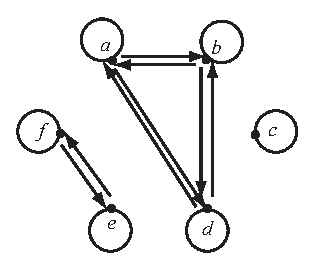
\includegraphics{figps-exer2-73.eps}}
\end{center}
\end{figure}
\end{list}


\begin{list}{\bf{\ref{exer:sec73-2}.}}
\item Let $x \in A$.  Since $x$ has the same number of digits as itself, the relation $\mathrel{R}$ is reflexive.  Now let $x, y, z \in A$.  If $x \mathrel{R} y$, then $x$  and  $y$  have the same number of digits.  Hence, $y$ and $x$ have the same number of digits and $y \mathrel{R} x$, and so $\mathrel{R}$ is symmetric.

If $x \mathrel{R} y$ and $y \mathrel{R} z$, then $x$  and  $y$  have the same number of digits and 
$y$  and  $z$  have the same number of digits.  Hence, $x$  and  $z$  have the same number of digits, and so $x \mathrel{R} z$.  Therefore, $\mathrel{R}$ is transitive.

The equivalence classes are:  
$\left\{ 0, 1, 2, \ldots , 9 \right\}$, $\left\{ 10, 11, 12, \ldots , 99 \right\}$, \\
$\left\{ 100, 101, 102, \ldots , 999 \right\}$, $\left\{ 1000 \right\}$.
\end{list}



\begin{list}{\bf{\ref{exer:sec73-congclass}.}}
\item The congruence classes for the relation of congruence modulo 5 on the set of integers are

\begin{multicols}{2}$\left[ 0 \right] = \left\{ 5n \mid n \in \mathbb{Z} \right\}$

$\left[ 1 \right] = \left\{ 5n +1 \mid n \in \mathbb{Z} \right\}$

$\left[ 2 \right] = \left\{ 5n + 2 \mid n \in \mathbb{Z} \right\}$

$\left[ 3 \right] = \left\{ 5n + 3 \mid n \in \mathbb{Z} \right\}$

$\left[ 4 \right] = \left\{ 5n + 4 \mid n \in \mathbb{Z} \right\}$.
\end{multicols}
\end{list}


\begin{list}{\bf{\ref{exer:modpowers}.}}
\item \begin{list}{\bf{(a)}}
\item Let $a, b, c \in \Z_9$.  Since $a^2 \equiv a^2 \pmod 9$, we see that $a \sim a$ and $\sim$ is reflexive.  Let $a, b, c \in \Z_9$.  If $a \sim b$, then $a^2 \equiv b^2 \pmod 9$ and hence, by the symmetric property of congruence, $b^2 \equiv a^2 \pmod 9$.  This proves that $\sim$ is symmetric.  Finally, if $a \sim b$ and $b \sim c$, then 
$a^2 \equiv b^2 \pmod 9$ and $b^2 \equiv c^2 \pmod 9$.  By the transitive property of congruence, we conclude that $a^2 \equiv c^2 \pmod 9$ and hence, $a \sim c$.  This proves that $\sim$ is transitive.  The distinct equivalence classes are $\left\{0, 3, 6 \right\}$, $\left\{1, 8 \right\}$, 
$\left\{ 2, 7 \right\}$, and $\left\{ 4, 5 \right\}$.
\end{list}
\end{list}


\begin{list}{\bf{\ref{exer:sec73-integer}.}}
\item \begin{list}{\bf{(a)}}
\item Let $x \in \left[ \dfrac{5}{7} \right]$.  Then $x - \dfrac{5}{7} \in \Z$, which means that there is an integer $m$ such that $x - \dfrac{5}{7} = m$, or $x = \dfrac{5}{7} + m$.  This proves that \linebreak
$x \in \left\{ \left. m + \dfrac{5}{7} \right| m \in \Z \right\}$ and, hence, that
$\left[ \dfrac{5}{7} \right] \subseteq \left\{ \left. m + \dfrac{5}{7} \right| m \in \Z \right\}$.  We still need to prove that 
$\left\{ \left. m + \dfrac{5}{7} \right| m \in \Z \right\} \subseteq \left[ \dfrac{5}{7} \right]$.
\end{list}
\end{list}


\begin{list}{\bf{\ref{exer:sec73-rationals}.}}
\item \begin{list}{\bf{(a)}}
\item To prove the relation is symmetric, note that if $(a, b) \approx (c, d)$, then 
$ad = bc$.  This implies that $cb = da$ and, hence,  $(c, d) \approx (a, b)$.
\end{list}
\end{list}


\begin{list}{}
\item \begin{list}{\bf{(c)}}
\item $3a = 2b$
\end{list}
\end{list}

\hbreak
\endinput



\section*{Section \ref{S:modulararithmetic}}

\begin{list}{\bf{\ref{exer:sec74-modtables}.}}
\item \begin{list}{\bf{(a)}}
\item
\begin{tabular}{ c | c  c  c  c  p{0.5in} c | c  c  c  c}
$\oplus$ & $[ 0 ]$ & $[ 1 ]$ & $[ 2 ]$ & $[ 3 ]$ & 
  & $\odot$ & $[ 0 ]$ & $[ 1 ]$ & $[ 2 ]$ & $[ 3 ]$   \\ \cline{1-5} \cline{7-11}

$[ 0 ]$ & $[ 0 ]$ & $[ 1 ]$ & $[ 2 ]$ & 
$[ 3 ]$ & & $[ 0 ]$ & $[ 0 ]$ & 
$[ 0 ]$ & $[ 0 ]$ & $[ 0 ]$  
\\ 

$[ 1 ]$ & $[ 1 ]$ & $[ 2 ]$ & $[ 3 ]$ & 
$[ 0 ]$ & & $[ 1 ]$ & $[ 0 ]$ & 
$[ 1 ]$ & $[ 2 ]$ & $[ 3 ]$ \\ 

$[ 2 ]$ & $[ 2 ]$ & $[ 3 ]$ & $[ 0 ]$ & 
$[ 1 ]$ & & $[ 2 ]$ & $[ 0 ]$ & 
$[ 2 ]$ & $[ 0 ]$ & $[ 2 ]$ \\ 

$[ 3 ]$ & $[ 3 ]$ & $[ 0 ]$ & $[ 1 ]$ & 
$[ 2 ]$ & & $[ 3 ]$ & $[ 0 ]$ & 
$[ 3 ]$ & $[ 2 ]$ & $[ 1 ]$ \\ 
\end{tabular}
\end{list}
\end{list}
\vskip6pt

\begin{list}{}
\item \begin{list}{\bf{(b)}}
\item \begin{tabular}{ c | c  c  c  c  c  c  c}
$\oplus$ & $[ 0 ]$ & $[ 1 ]$ & $[ 2 ]$ & $[ 3 ]$ & 
$[ 4 ]$ & $[ 5 ]$ & $[ 6 ]$  \\ \hline

$[ 0 ]$ & $[ 0 ]$ & $[ 1 ]$ & $[ 2 ]$ & 
$[ 3 ]$ & $[ 4 ]$ & $[ 5 ]$ & $[ 6 ]$  \\ 

$[ 1 ]$ & $[ 1 ]$ & $[ 2 ]$ & $[ 3 ]$ & 
$[ 4 ]$ & $[ 5 ]$ & $[ 6 ]$ & $[ 0 ]$  \\ 

$[ 2 ]$ & $[ 2 ]$ & $[ 3 ]$ & $[ 4 ]$ & 
$[ 5 ]$ & $[ 6 ]$ & $[ 0 ]$ & $[ 1 ]$  \\ 

$[ 3 ]$ & $[ 3 ]$ & $[ 4 ]$ & $[ 5 ]$ & 
$[ 6 ]$ & $[ 0 ]$ & $[ 1 ]$ & $[ 2 ]$ \\ 

$[ 4 ]$ & $[ 4 ]$ & $[ 5 ]$ & $[ 6 ]$ & 
$[ 0 ]$ & $[ 1 ]$ & $[ 2 ]$ & $[ 3 ]$  \\ 

$[ 5 ]$ & $[ 5 ]$ & $[ 6 ]$ & $[ 0 ]$ & 
$[ 1 ]$ & $[ 2 ]$ & $[ 3 ]$ & $[ 4 ]$  \\ 

$[ 6 ]$ & $[ 6 ]$ & $[ 0 ]$ & $[ 1 ]$ & 
$[ 2 ]$ & $[ 3 ]$ & $[ 4 ]$ & $[ 5 ]$  \\ 
\end{tabular}

\vskip9pt

\begin{tabular}{ c | c  c  c  c  c  c  c}
$\odot$ & $[ 0 ]$ & $[ 1 ]$ & $[ 2 ]$ & $[ 3 ]$ & 
$[ 4 ]$ & $[ 5 ]$ & $[ 6 ]$  \\ \hline

$[ 0 ]$ & $[ 0 ]$ & $[ 0 ]$ & $[ 0 ]$ & 
$[ 0 ]$ & $[ 0 ]$ & $[ 0 ]$ & $[ 0 ]$  \\ 

$[ 1 ]$ & $[ 0 ]$ & $[ 1 ]$ & $[ 2 ]$ & 
$[ 3 ]$ & $[ 4]$ & $[ 5 ]$ & $[ 6 ]$  \\ 

$[ 2 ]$ & $[ 0 ]$ & $[ 2 ]$ & $[ 4 ]$ & 
$[ 6 ]$ & $[ 1 ]$ & $[ 3 ]$ & $[ 5 ]$  \\ 

$[ 3 ]$ & $[ 0 ]$ & $[ 3 ]$ & $[ 6 ]$ & 
$[ 2 ]$ & $[ 5 ]$ & $[ 1 ]$ & $[ 4 ]$  \\ 

$[ 4 ]$ & $[ 0 ]$ & $[ 4 ]$ & $[ 1 ]$ & 
$[ 5 ]$ & $[ 2 ]$ & $[ 6 ]$ & $[ 3 ]$  \\ 

$[ 5 ]$ & $[ 0 ]$ & $[ 5 ]$ & $[ 3 ]$ & 
$[ 1 ]$ & $[ 6 ]$ & $[ 4 ]$ & $[ 2 ]$  \\ 

$[ 6 ]$ & $[ 0 ]$ & $[ 6 ]$ & $[ 5 ]$ & 
$[ 4 ]$ & $[ 3 ]$ & $[ 2 ]$ & $[ 1 ]$  \\ 
\end{tabular}
\end{list}
\end{list}

%\begin{list}{\ref{exer:sec74-modtables}.}
%\item \begin{list}{(a)}
%\item \begin{tabular}[t]{ c | c  c  p{0.5in} c | c  c}
%$\oplus$ & $[ 0 ]$ & $[ 1 ]$ &  & $\odot$ & $[ 0 ]$ & $[ 1 ]$ \\ \cline{1-3} \cline{5-7}
%
%$[ 0 ]$ & $[ 0 ]$ & $[ 1 ]$ &  & $[ 0 ]$ & $[ 0 ]$ & $[ 0 ]$ \\ 
%
%$[ 1 ]$ & $[ 1 ]$ & $[ 0 ]$ &  & $[ 1 ]$ & $[ 0 ]$ & $[ 1 ]$ \\ 
%\end{tabular}
%
%\end{list}
%\end{list}
%\vskip6pt
%
%\begin{list}{}
%\item \begin{list}{(b)}
%\item \begin{tabular}[t]{ c | c  c  c  p{0.5in} c | c  c  c}
%$\oplus$ & $[ 0 ]$ & $[ 1 ]$ & $[ 2 ]$ & &   $\odot$ & $[ 0 ]$ & $[ 1 ]$ & $[ 2 ]$   \\ \cline{1-4} \cline{6-9}
%
%$[ 0 ]$ & $[ 0 ]$ & $[ 1 ]$ & $[ 2 ]$ &  & 
%$[ 0 ]$ & $[ 0 ]$ & $[ 0 ]$ & $[ 0 ]$  
%\\ 
%
%$[ 1 ]$ & $[ 1 ]$ & $[ 2 ]$ & $[ 0 ]$ &  & 
%$[ 1 ]$ & $[ 0 ]$ & $[ 1 ]$ & $[ 2 ]$ 
%\\ 
%
%$[ 2 ]$ & $[ 2 ]$ & $[ 0 ]$ & $[ 1 ]$ &  & 
%$[ 2 ]$ & $[ 0 ]$ & $[ 2 ]$ & $[ 1 ]$  
%\\ 
%\end{tabular}
%\end{list}
%\end{list}
%\vskip6pt


\begin{multicols}{2}
\begin{list}{\bf{\ref{exer:sec74-3}.}}
\item \begin{list}{\bf{(a)}}
\item $[ x ] = [ 1 ]$ or $[ x ] = [ 3 ]$ \qquad 
%(e) $[ x ] = [ 2 ]$ or $[ x ] = [ 3 ]$
\end{list}
\end{list}

\begin{list}{}
\item \begin{list}{\bf{(e)}}
\item $[ x ] = [ 2 ]$ or $[ x ] = [ 3 ]$
\end{list}
\end{list}
\end{multicols}

\begin{list}{}
\item \begin{list}{\bf{(g)}}
\item The equation has no solution.
\end{list}
\end{list}

\begin{list}{\bf{\ref{exer:sec74-4}.}}
\item \begin{enumerate}
\item The statement is false.  By using the multiplication table for $\mathbb{Z}_6$, we see that a counterexample is $\left[ a \right] = \left[ 2 \right]$.

\item The statement is true.  By using the multiplication table for $\mathbb{Z}_5$, we see that:

\begin{multicols}{2}
\begin{list}{}
\item $\left[ 1 \right] \odot \left[ 1 \right] = \left[ 1 \right]$.

\item $\left[ 2 \right] \odot \left[ 3 \right] = \left[ 1 \right]$.

\item $\left[ 3 \right] \odot \left[ 2 \right] = \left[ 1 \right]$.

\item $\left[ 4 \right] \odot \left[ 4 \right] = \left[ 1 \right]$.
\end{list}
\end{multicols}
\end{enumerate}
\end{list}





\begin{list}{\bf{\ref{exer:squaresinZ5}.}}
\item \begin{list}{\bf{(a)}}
\item The proof consists of the following computations:
\begin{multicols}{2}
\begin{list}{}
\item $[ 1 ]^2 = [ 1 ]$
\item $[ 2 ]^2 = [ 4 ]$
\item $[ 3 ]^2 = [ 9 ] = [ 4 ]$
\item $[ 4 ]^2 = [ 16 ] = [ 1 ]$.
\end{list}
\end{multicols}
\end{list}
\end{list}


\begin{list}{\bf{\ref{exer:sec74cong3}.}}
\item \begin{list}{\bf{(a)}}
\item Prove the contrapositive by calculating $[ a ]^2 + [ b ]^2$ for all nonzero $[ a ]$ and $[ b ]$ in $\Z_3$.
\end{list}
\end{list}
\hbreak
%\pagebreak
\endinput




\subsection*{Section \ref{S:gcd}}

\begin{list}{\bf{\ref{exer:sec81-1}.}}
\item \begin{enumerate}%\begin{multicols}{2}
\item The set of positive common divisors of 21 and 28 is $\{1, 7\}$.  So \\$\gcd ( {21, 28} ) = 7$.

\item The set of positive common divisors of $-21$ and 28 is $\{1, 7\}$.  So \\$\gcd ( { - 21, 28} ) = 7$.

\item The set of positive common divisors of 58 and 63 is $\{1 \}$.  So \\$\gcd ( {58, 63} ) = 1$.

\item The set of positive common divisors of 0 and 12 is $\{1, 2, 3, 4, 6, 12 \}$.  So $\gcd ( {0, 12} ) = 12$.
%\end{multicols}
\end{enumerate}
\end{list}


\begin{list}{\bf{\ref{exer:sec81-2}.}}
\item \begin{list}{\bf{(a)}}
\item \hint  Prove that $k \mid \left[ ( {a+1} ) - a \right]$.
\end{list}
\end{list}


\begin{list}{\bf{\ref{exer:sec81-props}.}}
\item \begin{list}{\bf{(a)}}
\item $|b|$ is the largest natural number that divides 0 and $b$.
\end{list}
\end{list}

\begin{list}{}
\item \begin{list}{\bf{(b)}}
\item The integers $b$ and $-b$ have the same divisors.  Therefore, 
$\gcd ( a, -b ) = \gcd ( a, b )$.
\end{list}
\end{list}


\begin{list}{\bf{\ref{exer:sec81-4}.}}
\item \begin{tabular}[t] {l l}
\textbf{(a)} $\gcd ( {36, 60} ) = 12$  & $12 = 36 \cdot 2 + 60 \cdot ( { - 1} )$ \\
\textbf{(b)} $\gcd ( {901, 935} ) = 17$	& $17 = 901 \cdot 27 + 935 \cdot ( { - 26} )$ \\
\textbf{(e)} $\gcd ( {901, -935} ) = 17$	& $17 = 901 \cdot 27 + (-935) \cdot ( { 26} )$ \\
\end{tabular}
\end{list}


\begin{list}{\bf{\ref{exer81:solvingeqn}.}}
\item \begin{list}{\bf{(a)}}
\item One possibility is $u = -3$ and $v = 2$.  In this case, $9u + 14v = 1$.  We then multiply both sides of this equation by 10 to obtain
\[
9 \cdot (-30) + 14 \cdot 20 = 10.
\]
So we can use $x = -30$ and $y = 20$.
\end{list}
\end{list}



\begin{multicols}{2}
\begin{list}{\bf{\ref{exer:gcdandfractions}.}}
\item \begin{list}{\bf{(a)}}
\item $11 \cdot (-3) + 17 \cdot 2 = 1$
\end{list}
\end{list}

\begin{list}{}
\item \begin{list}{\bf{(b)}}
\item $\dfrac{m}{11} + \dfrac{n}{17} = \dfrac{17m +11n}{187}$
\end{list}
\end{list}
\end{multicols}
\hbreak
\endinput



\subsection*{Section \ref{S:primefactorizations}}

\begin{list}{\bf{\ref{exer:sec82-1}.}}
\item For both parts, use the fact that the only natural number divisors of a prime number $p$ are 1 and $p$.
\end{list}

\begin{list}{\bf{\ref{exer:sec82-2}.}}
\item Use cases: (1) $p$ divides $a$; (2) $p$ does not divide $a$.  In the first case, the conclusion is automatically true.  For the second case, use the fact that $\gcd ( p, a ) = 1$ and so we can use Theorem~\ref{T:relativelyprimeprop} to conclude that $p$ divides $b$.  Another option is to write the number 1 as a linear combination of $a$ and $p$ and then multiply both sides of the equation by $b$.
\end{list}

\begin{list}{\bf{\ref{exer:sec82-3}.}}
\item A hint for the inductive step: Write  $p \mid ( {a_1 a_2  \cdots a_m } )a_{m + 1} $.  Then look at two cases:  (1) $p \mid a_{m + 1} $; (2) $p$  does not divide  $a_{m + 1} $.
\end{list}

\begin{list}{\bf{\ref{exer:lincombequalone}.}}
\item \begin{list}{\bf{(a)}}
\item $\gcd ( a, b ) = 1$.  Why?
\end{list}
\end{list}

\begin{list}{}
\item \begin{list}{(\bf{b)}}
\item $\gcd ( a, b ) = 1$ or $\gcd ( a, b ) = 2$.  Why?
\end{list}
\end{list}

\begin{list}{\bf{\ref{exer:dividebygcd}.}}
\item \begin{enumerate}
\item $\gcd \left( 16, 28 \right) = 4$.  Also, $\dfrac{16}{4} = 4$, $\dfrac{28}{4} = 7$, and 
$\gcd \left( 4, 7 \right) = 1$.

\item $\gcd \left( 10, 45 \right) = 5$.  Also, $\dfrac{10}{5} = 2$, $\dfrac{45}{5} = 9$, and 
$\gcd \left( 2, 9 \right) = 1$.
\end{enumerate}
\end{list}


\begin{list}{\bf{\ref{exer:24divides-nsquaredminus1}.}}
\item Part (b) of Exercise~(\ref{exer:sec82-truefalse}) can be helpful.
\end{list}


\begin{list}{\bf{\ref{exer:cdividessum}.}}
\item The statement is true.  Start of a proof:  If   $\gcd ( {a, b} ) = 1$  and  
$c \mid ( {a + b} )$, then there exist integers $x$ and $y$ such that 
$ax + by = 1$ and there exists an integer $m$ such that $a + b = cm$.  
%So, we can write 
%$b = cm - a$ and substitute this into the other equation.  This gives
%\[
%\begin{aligned}
%              ax + ( cm - a ) y &= 1 \\
%a ( x - y ) + c ( my ) &= 1. \\
%\end{aligned}
%\]
%This proves that $\gcd ( a, c ) = 1$.  A similar proof shows that 
%$\gcd ( b, c ) = 1$.
\end{list}
\hbreak
\pagebreak
\endinput



\subsection*{Section \ref{S:diophantine}}

\begin{multicols}{2}
\begin{list}{\bf{\ref{exer:sec83-2}.}}
\item \begin{list}{\bf{(a)}}
\item $x = -3 + 14k$, $y = 2 - 9k$
\end{list}
\end{list}

\begin{list}{}
\item \begin{list}{\bf{(b)}}
\item $x = -1 + 11k$, $y = 1 - 9k$
\end{list}
\end{list}

\begin{list}{}
\item \begin{list}{\bf{(c)}}
\item No solution
\end{list}
\end{list}

\begin{list}{}
\item \begin{list}{\bf{(d)}}
\item $x = 2+3k$, $y = -2-4k$
\end{list}
\end{list}
\end{multicols}


\begin{list}{\bf{\ref{exer:balancing}.}}
\item There are several possible solutions to this problem, each of which can be generated from the solutions of the Diophantine equation \linebreak
$27x + 50y = 25$.
\end{list}

\begin{list}{\bf{\ref{exer:sec83-5}.}}
\item This problem can be solved by finding all solutions of a linear Diophantine equation $25x + 16y = 1461$, where both $x$ and $y$ are positive.  The mininum number of people attending the banquet is 66.
\end{list}

\begin{list}{\bf{\ref{exer:lindioph3}.}}
\item \begin{enumerate}
\item $y = 12 + 16k, x_3 = -1 - 3k$

\item If $3y = 12x_1 + 9x_2$ and $3y + 16x_3 = 20$, we can substitute for $3y$ and obtain 
$12x_1 + 9x_2 + 16x_3 = 20$.

\item Rewrite the equation $12x_1 + 9x_2 = 3y$ as $4x_1 + 3x_2 = y$.  A general solution for this linear Diophantine equation is
\begin{align*}
x_1 &= y + 3n \\
x_2 &= -y - 4n. \\
\end{align*}
\end{enumerate}
\end{list}
\hbreak
\endinput




\subsection*{Section~\ref{S:finitesets}}

\begin{list}{\bf{\ref{exer:sec92-1}.}}
\item One way to do this is to prove that the following function is a bijection:  $f\x A \times \left\{ x \right\} \to A$ by $f ( a, x ) = a$, for all 
$( a, x ) \in A \times \left\{ x \right\}$.
\end{list}


\begin{list}{\bf{\ref{exer91:evennaturals}.}}
\item One way to prove that $\N \approx E^+$ is to find a bijection from $\N$ to $E^+$.  One possibility is $f: \mathbb{N} \to E^+$ by $f \left( n \right) = 2n$ for all $n \in \mathbb{N}$.  (We must prove that this is a bijection.)
\end{list}


\begin{list}{\bf{\ref{exer:sec92corollary}.}}
\item Notice that $A = ( A - \left\{ x \right\} ) \cup \left\{x \right\}$.  Use 
Theorem~\ref{T:finitesubsets} to conclude that $A - \left\{ x \right\}$ is finite.  Then use 
Lemma~\ref{L:addone}.
\end{list}


\begin{list}{\bf{\ref{exer:sec92-finitesets}.}}
\item \begin{enumerate}
\item Since $A \cap B \subseteq A$, if $A$ is finite, then Theorem~\ref{T:finitesubsets} implies that $A \cap B$ is finite.
\item The sets $A$ and $B$ are subsets of $A \cup B$.  So if $A \cup B$ is finite, then $A$ and $B$ are finite.
\end{enumerate}
\end{list}


\begin{list}{\bf{\ref{exer:sec92-7}.}}
\item \begin{list}{\bf{(a)}}
\item Remember that two ordered pairs are equal if and only if their corresponding coordinates are equal.  So if $\left( a_1, c_1 \right) , \left( a_2, c_2 \right) \in A \times C$ and $h \left( a_1, c_1 \right) = h \left( a_2, c_2 \right)$, then 
$\left( f \left( a_1 \right), g \left( c_1 \right) \right) = 
\left( f \left( a_2 \right), g \left( c_2 \right) \right)$.  We can then conclude that 
$f \left( a_1 \right) = f \left( a_2 \right)$ and $g \left( c_1 \right) = g \left( c_2 \right)$.  Since $f$ and $g$ are both injections, this means that $a_1 = a_2$ and $c_1 = c_2$ and therefore, 
$\left( a_1, c_1 \right) = \left( a_2, c_2 \right)$.  This proves that $f$ is an injection.

Now let $\left( b, d \right) \in B \times D$.  Since $f$ and $g$ are surjections, there exists 
$a \in A$ and $c \in C$ such that $f \left( a \right) = b$ and $g \left( c \right) = d$.  Therefore, $h \left( a, c \right) = \left( b, d \right)$.  This proves that $f$ is a surjection.
\end{list}
\end{list}


\begin{list}{\bf{\ref{exer:sec927}.}}
\item \begin{list}{\bf{(a)}}
\item If we define the function $f$ by $f ( 1 ) = a$, $f ( 2 ) = b$, 
$f ( 3 ) = c$, $f ( 4 ) = a$, and $f ( 5 ) = b$, then we can use 
 $g ( a ) = 1$, $g ( b ) = 2$, and $g ( 3 ) = c$.  The function $g$ is an injection.
\end{list}
\end{list}




\hbreak

\endinput



\subsection*{Section~\ref{S:infinitesets}}

\begin{list}{\bf{\ref{exer:sec93-1}.}}
\item All except Part~(d) are true.
\end{list}



\begin{list}{\bf{\ref{exer:sec93-2}.}}
\item \begin{enumerate}
\item Prove that the function $f: \mathbb{N} \to F^+$ defined by $f \left( n \right) = 5n$ for all 
$n \in \mathbb{N}$ is a bijection. 
\setcounter{enumi}{4}
\item  One way is to define $f\x \N \to \N -\{4, 5, 6 \}$ by
\begin{equation} \notag
f( n ) = 
\begin{cases}
n                        &\text{if $n = 1$, $n = 2$, or $n = 3$} \\
f ( n + 3 )   &\text{if $n \geq 4$}.
\end{cases}
\end{equation}
and then prove that the function $f$ is a bijection.

It is also possible to use Corollary~\ref{C:subsetofcountable} to conclude that $\mathbb{N} - \left\{ 4, 5, 6 \right\}$ is countable, but it must also be proved that $\mathbb{N} - \left\{ 4, 5, 6 \right\}$ cannot be finite.  To do this, assume that $\mathbb{N} - \left\{ 4, 5, 6 \right\}$ is finite and then prove that $\N$ is finite, which is a contradiction.
\item  Let $A = \left\{ m \in \mathbb{Z} \mid m \equiv 2 \pmod 3 \right\} = 
\left\{ 3k + 2 \mid k \in \mathbb{Z} \right\}$.  Prove that the function $f: \mathbb{Z} \to A$ is a bijection, where $f \left( x \right) = 3x + 2$ for all $x \in \mathbb{Z}$.  This proves that 
$\mathbb{Z} \approx A$ and hence, $\mathbb{N} \approx A$.
\end{enumerate}
\end{list}



\begin{list}{\bf{\ref{exer:addfinitetocountable}.}}
\item For each $n \in \mathbb{N}$, let $P ( n )$ be ``If 
$\text{card} ( B ) = n$, then $A \cup B$ is a countably infinite set.''

Note that if $\text{card} ( B ) = k+1$ and $x \in B$, then 
$\text{card} ( B - \left\{ x \right\} ) = k$.  Apply the inductive assumption to 
$B - \left\{ x \right\}$.
\end{list}



\begin{list}{\bf{\ref{exer:unionofcountable}.}}
\item Let $m, n \in \mathbb{N}$ and assume that $h \left( n \right) = h \left( m \right)$. Then since $A$ and $B$ are disjoint, either $h \left( n \right)$ and $h \left( m \right)$ are both in $A$ or are both in $B$.  If they are both in $A$, then both $m$ and $n$ are odd and
\[
f \left( \frac{n + 1}{2} \right) = h \left( n \right) = h \left( m \right) = f \left( \frac{m + 1}{2} \right).
\]
Since $f$ is an injection, this implies that $\dfrac{n + 1}{2} = \dfrac{m + 1}{2}$ and hence that $n = m$.  Similary, if both $h \left( n \right)$ and $h \left( m \right)$ are in $B$, then $m$ and $n$ are even and $g \left( \dfrac{n}{2} \right) = g \left( \dfrac{m}{2} \right)$, and since $g$ is an injection, $\dfrac{n}{2} = \dfrac{m}{2}$ and $n = m$.  Therefore, $h$ is an injection.

Now let $y \in A \cup B$.  There are only two cases to consider:  $y \in A$ or $y \in B$.  If 
$y \in A$, then since $f$ is a surjection, there exists an $m \in \mathbb{N}$ such that 
$f \left( m \right) = y$.  Let $n = 2m - 1$.  Then $n$ is an odd natural number, 
$m = \dfrac{n + 1}{2}$,  and
\[
h \left( n \right) = f \left( \frac{n + 1}{2} \right) = f \left( m \right) = y.
\]
Now assume $y \in B$ and use the fact that $g$ is a surjection to help prove that there exists a natural number $n$ such that $h(n) = y$.

%If $y \in B$, then since $g$ is a surjection, there exists an $m \in \mathbb{N}$ such that 
%$g \left( m \right) = y$.  Let $n = 2m$.  Then $n$ is an even natural number, 
%$m = \dfrac{n}{2}$,  and
%\[
%h \left( n \right) = g \left( \frac{n}{2} \right) = g \left( m \right) = y.
%\]
We can then conclude that $h$ is a surjection.
%\item Notice that if $h ( n ) = h ( m )$, then since $A$ and $B$ are disjoint, either $h ( n )$ and $h ( m )$ are both in $A$ or are both in $B$.
%
%Also, if $y \in A \cup B$, then there are only two cases to consider:  $y \in A$ or $y \in B$.
\end{list}


\begin{list}{\bf{\ref{exer:Qiscountable}.}}
\item By Theorem~\ref{T:positiverationals}, the set $\mathbb{Q}^+$ of positive rational numbers is countably infinite. So by Theorem~\ref{T:addonetocountable}, 
$\mathbb{Q}^+ \cup \left\{ 0 \right\}$ is countably infinite.  Now prove that the set $\mathbb{Q}^-$ of all negative rational numbers is countably infinite and then use  Theorem~\ref{T:unionofcountable} to prove that $\mathbb{Q}$ is countably infinite.

\end{list}

\begin{list}{\bf{\ref{exer:countinf-finite}.}}
\item Since $A - B \subseteq A$, the set $A - B$ is countable.  Now assume $A - B$ is finite and show that this leads to a contradiction.
\end{list}
\hbreak

\endinput



\subsection*{Section~\ref{S:uncountablesets}}

\begin{list}{\bf{\ref{exer:sec94-1}.}}
\item \begin{list}{\bf{(a)}}
\item One such bijection is $f\x ( 0, \infty ) \to \mathbb{R}$ by $f ( x ) = \ln x$ for all 
$x \in ( 0, \infty )$
\end{list}
\end{list}

\begin{list}{}
\item \begin{list}{\bf{(b)}}
\item One such bijection is $g\x ( 0, \infty ) \to ( a, \infty )$ by $g( x ) = x + a$ for all $x \in ( 0, \infty )$.  The function $g$ is a bijection and so 
$\left( 0, \infty \right) \approx \left( a, \infty \right)$.  Then use Part~(a).
%\item Find a bijection from $\left( 0, \infty \right)$ to  $\left( a, \infty \right)$.
\end{list}
\end{list}


\begin{list}{\bf{\ref{exer:irrationaluncount}.}}
\item Use a proof by contradiction.  Let $\mathbb{H}$ be the set of irrational numbers and assume that $\mathbb{H}$ is countable.  Then 
$\mathbb{R} = \mathbb{Q} \cup \mathbb{H}$ and $\mathbb{Q}$ and $\mathbb{H}$ are disjoint.  Use Theorem~\ref{T:unionofcountable}, to obtain a contradiction.
\end{list}


\begin{list}{\bf{\ref{exer:supersetofuncount}.}}
\item By Corollary~\ref{C:subsetofcountable}, every subset of a countable set is countable.  So if 
$B$ is countable, then $A$ is countable. %Use Corollary~\ref{C:subsetofcountable} on page~\pageref{C:subsetofcountable}.
\end{list}


\begin{list}{\bf{\ref{exer93:uncountablesets}.}}
\item By Cantor's Theorem (Theorem~\ref{T:cantor}), $\mathbb{R}$ and 
$\mathcal{P} \left( \mathbb{R} \right)$ do not have the same cardinality.
\end{list}

\hbreak
\endinput


\endinput



\setcounter{page}{3}
\part{Using the Text}
\label{part:usingtext}%
\markboth{Using the Text}{Using the Text}



\emph{Mathematical Reasoning and Writing} was written to assist students with the transition from calculus to upper level mathematics courses.  Students should be able to effectively use this text with a background of one semester of calculus.  Following are some of the important ways this text will help with this transition.

\section*{Emphasis on Writing in Mathematics}

\subsection*{The Writing Guidelines}

The issue of writing mathematical exposition is addressed throughout the book.  Guidelines for writing mathematical proofs are incorporated into the book.  These guidelines are introduced when needed and begin in Chapter~\ref{C:intro}.  Appendix~\ref{C:writingguides} contains a summary of all the guidelines for writing mathematical proofs that are introduced in the text.  In addition, every attempt has been made to insure that each proof presented in this text is written according to these guidelines.  This provides students with examples of well-written proofs.

\vskip6pt
Some of the writing guidelines deal with the use of a word processor.  At Grand Valley State University, this text has been used for several years for a course called ``Communicating in Mathematics.''  It is a sophomore level course with a Calculus I prerequisite that is required for all mathematics majors and minors.  For this course, the Department of Mathematics requires that students use a word processor capable of producing the appropriate mathematical symbols and equations.  (Microsoft Word and its equation editor is available on the student network.)  However, the writing guidelines can easily be implemented for courses where students do not have access to this type of word processing.

\subsection*{A Writing Assignment}

At Grand Valley, we do not require that every proof a student completes must be written on a word processor.  There is one major assignment where a word processor is required.  Many of us call this the ``Proofs Portfolio.''  Since our course is part of the University's Writing Skills Program, students must have an opportunity to work on a writing assignment, get feedback from the instructor, and then have the opportunity to revise their work.  We use the ``Proofs Portfolio'' to satisfy this requirement.  This portfolio consists of ten proofs (or propositions to be proven or disproven).  Students may hand in each proof to the professor two times to be critiqued.  Most of the critique is directed toward the student's writing, but we must occasionally give some ``mathematical direction'' to the student.  However, most of the time this is quite general, such as, ``You have an algebra mistake here.''

\vskip6pt
The goal is that each student will have a completed ``Portfolio of Proofs'' at the end of the semester.  The eight to ten proofs in the portfolio are chosen to illustrate the various proof techniques discussed in the course.  Hopefully, the students will be able to use their portfolios to provide examples of various proof techniques if they are required in later courses.

\vskip6pt
Sample instructions and sample portfolio problems that I have used are given later in this part of the Instructor's Manual.
\hbreak


\section*{Instruction in the Process of Constructing Proofs}

One of the primary goals of this book is to develop a student's ability to construct mathematical proofs and then to write the proof in a coherent manner that conveys an understanding of the proof to the reader.  These are two distinct skills.  Instruction on how to write proofs begins in Section~\ref{S:direct} and is developed further in Chapter~\ref{C:proofs}.  In addition, Chapter~\ref{C:induction} is devoted to developing students' abilities to construct proofs using mathematical induction.  

\subsection*{Know-Show Tables}

Students are taught to organize their thought processes when attempting to construct a proof with a so-called ``know-show table.'' (See Section~\ref{S:direct} and Section~\ref{S:directproof}.)  Students use this table to work backward from what it is they are trying to prove while at the same time working forward from the assumptions of the problem.  The know-show tables are used quite extensively in Chapter~\ref{C:proofs}.  However, the text gradually decreases the explicit use of know-show tables in the later chapters.  One reason for this is that these tables may work well when there appears to be only one way of proving a certain result.  As the proofs become more complicated or other methods of proof (such as proofs using cases) are used, these know-show ables become less useful.


So, the know-show ables are not to be considered an absolute necessity in using the text.  However, they are useful for students beginning to learn how to construct and write proofs.  They provide a convenient way for students to organize their work.  More importantly, they introduce students to a way of thinking about a problem.  Instead of immediately trying to write a complete proof, the know-show table forces students to stop, think, and ask questions such as:

\begin{itemize}
\item Just exactly what is it that I am trying to prove?
\item How can I prove this?
\item What methods do I have that may allow me to prove this?
\item What are the assumptions?
\item How can I use these assumptions to prove the result?
\end{itemize}

Being able to ask these questions is a big step in constructing a proof.  The next task is to answer the questions and to use those answers to construct a proof.
\hbreak

\section*{Emphasis on Active Learning}

One of the underlying premises of this text is that the best way to learn and understand mathematics is to be actively involved in the learning process.  However, it is unreasonable to expect students to just go out and learn mathematics on their own.  Students actively involved in learning mathematics need appropriate materials that will provide guidance and support in their learning of mathematics.  This text provides these by incorporating two or three preview activities for each section and some activities within each section based on the material in that section.  These activities can be done individually or in a collaborative learning setting where students work in groups to brainstorm, make conjectures, test each others' ideas, reach consensus, and hopefully, to develop sound mathematical arguments to support their work.

\subsection*{Using and Grading the Preview Activities}

I require students to complete all the preview activities for a section prior to the classroom discussion of that section.  However, it is quite possible to have students complete one of the preview activities in class (perhaps in small groups) prior to the discussion.  It would also be possible to incorporate the material in one or two of the preview activities into a classroom discussion or lecture.

I do not grade all the preview activities.  Although students are required to complete all of them, on the day of class, I announce which one of the them I will collect and grade.  Grading is not based on whether or not everything is correct, but rather on whether or not a serious and substantial effort was made to complete the preview activities.  Each Preview Activity that is graded will receive a score of 4 points, 2 points, or 0 points.  This provides enough incentive for students to complete the preview activities without burdening me with an enormous amount of grading.  I can usually grade a preview activity in ten to fifteen minutes.  

The grading is also made easier by the fact that I distribute solutions to the preview activities for a section after the one is handed in.  I usually do this by posting the solutions on my web page.  The Instructor's Manual for this text contains the solutions of all preview activities and Adobe pdf files containing the solutions are available to the instructor.

However it is done, the Preview Activities at the beginning of each section should be completed by the students prior to the classroom discussion of the section.  The purpose of the preview activities is to prepare the students for the classroom discussion of the section.  By completing these preview activities, the students will be better prepared to participate in the classroom discussion.  Some preview activities will review prior mathematical work that is necessary for the new section.  This prior work may contain material from previous mathematical courses or it may contain material covered earlier in this text.  Other preview activities will introduce new concepts and definitions that will be used when that section is discussed in class.

\subsection*{Using the Progress Checks}
Students should work on the progress checks as they are studying the material in the book.  The progress checks are either short exercises or short activities designed to help the students determine if they are understanding the material as it is presented.  Some progress checks are also intended to prepare the student for the next topic in the section.  Answers to the Progress Checks are provided at the end of each chapter.

%\hbreak

\subsection*{Using the Activities}

In addition to the Preview Activities, each section of the text contains one or two activities related to the material contained in that section.  These activities are located at the end of each section and can be used for in-class group work or can be assigned as homework in addition to the exercises at the end of each section.  Most of the activities are optional, but they do provide useful work and sometimes thought provoking material.  The instructor must choose which activities to do in class and which to assign for out of class work.  Comments about using each activity is included in Part~\ref{part:activities} of this manual.
\hbreak

%\item \textbf{Mathematical Content}

%Mathematical content is needed as a vehicle for learning how to construct and write proofs.  The mathematical content for this text is drawn primarily from elementary number theory including congruence arithmetic; elementary set theory; functions, including injections, surjections, and the inverse of a function; and relations and equivalence relations.  This material is needed for upper level mathematics courses.

\section*{The Role of Logic}

In order to learn how to construct mathematical proofs, students need to learn some logic and gain experience in the traditional language and proof methods used in mathematics.  Since this is a text that deals with constructing and writing mathematical proofs, the logic that is presented is intended to aid in the construction of proofs.  The goals are to provide students with a thorough understanding of conditional statements, quantifiers, and logical equivalencies.  Emphasis is placed on writing correct and useful negations of statements, especially those involving quantifiers.  The logical equivalencies that are presented are those that provide the logical basis for some of the standard proof techniques such as proving the contrapositive, proof by contradiction, and proof using cases.
\hbreak

\section*{An Example of a Course Schedule}
As is mentioned in the Preface of the text, the chapters in the text can roughly be divided into the following (possibly overlapping) classes:

\begin{itemize}
\item Constructing and Writing Proofs:  Chapters~\ref{C:intro}, \ref{C:proofs}, and~\ref{C:induction}
\item Content: Chapters~\ref{C:settheory}, \ref{C:functions}, \ref{C:equivrelations}, \ref{C:numbertheory}, and~\ref{C:topicsinsets}
\item Logic: Chapter~\ref{C:logic}
\end{itemize}

A standard one-semester course in constructing and writing proofs should cover the first six chapters of the text and at least one of Chapter~\ref{C:equivrelations}, Chapter~\ref{C:numbertheory}, or Chapter~\ref{C:topicsinsets}.  A class consisting of well-prepared and motivated students could cover two of the last three chapters.  In addition, there are a few options that an instructor could choose to tailor the course to her or his needs.  For example,

\begin{itemize}
\item Chapter~\ref{C:induction} can be covered before Chapter~\ref{C:settheory} if it is desired to cover all methods of proof before beginning the ``content'' portion of the course.  The only part of Chapter~\ref{C:induction} that would need to be skipped is the material in Section~\ref{S:otherinduction} dealing with the cardinality of the power set.  If desired, this material could be included when the power set is discussed in Chapter~\ref{C:settheory}.

\item Instructors who would like to cover topics in both Chapters~\ref{C:equivrelations} and~\ref{C:numbertheory} can omit a few selected sections from earlier chapters.  Although it is an important and interesting section, Section~\ref{S:recursion} is not used in the remainder of the book.  The same is true for Section~\ref{S:inversefunctions}.  Finally, 
Section~\ref{S:constructive} can be skipped as long as the concept of a constructive proof is discussed during other parts of the course.
\end{itemize}

Following is a way I have implemented a schedule for a one-semester course that meets 3 times per week for 50 minutes for 14 weeks.  This schedule includes the material from Chapters~1 through~6 and Chapter 7.  It is possible to substitute Chapter~8 or Chapter~9 for Chapter~7.

\begin{center}
\begin{tabular}[h]{| c | c | c | l |} \hline
     &  Previews &            &            \\
 Day &  Due      &  In Class  &  Exercises \\  \hline
  1  &           &  Section 1.1 &            \\  
     &           &  Preview 1   &            \\ \hline
  2  &  Section 1.1  &  Section 1.1  &  1, 2, 4, 5, (6, 7, or 8), 9  \\ \hline
  3  &  Section 1.2  &  Section 1.2  &  1, 2, 3(b), 4, 5(a), 6, 7, 9, 10(a)\\ \hline
     &               &               &               \\ \hline
  4  &  Section 2.1  &  Section 2.1  &  1, 3, 4, 5  \\ \hline
  5  &  Section 2.2  &  Section 2.2  &  1, 2, 4, 5, 6, 7, 8  \\ \hline
  6  &  Section 2.3  &  Section 2.3  &  1, 2, 3, 4(a),5(a), 6, 7, 8, 9 \\
     &               &               &                 \\ \hline
     &               &               &                 \\ \hline
  7  &  Section 2.4  &  Section 2.4  &  1(a, b, d), 2(a, c, d, f, h), \\
     &               &               &  3(b, c, f), 4(b, c, f), 6 \\ \hline
  8  &               &  Section 2.4  &  \\
     &  Section 3.1  &  Section 3.1  &  1(a), 3, 4  \\ \hline
  9  &               &  Section 3.1  &  6, 7, 9, 10  \\ \hline
     &               &               &  \\ \hline
 10  &               &  Section 3.1  &  11(a)  \\
     &  Section 3.2  &  Section 3.2  &  1, 2, 4 \\ \hline
 11  &               &  Section 3.2  &  6, 7, 9  \\ \hline
 12  &  Section 3.3  &  Section 3.3  &  2, 3, 4, 6  \\ \hline
     &               &               &   \\ \hline
 13  &               &  Section 3.3  &  9, 10, 12  \\ \hline
 14  &  Section 3.4  &  Section 3.4  &  1, 2, 3, 6 \\ \hline
 15  &  Section 3.5  &  Section 3.4  &  7, 8, 10, 14  \\
     &               &  Section 3.5  &  1, 4, 5  \\ \hline
     &               &               &  \\ \hline
 16  &               &  Section 3.5  &  6, 8  \\
     &               &  Review       &  \\ \hline
 17  &               &  Test \#1     &  \\ \hline
 18  &  Section 4.1  &  Section 4.1  &  1, 2, 3, 5, 6, 7, 8, 10, 12  \\ \hline
     &               &               &  \\ \hline
 19  &  Section 4.2  &  Section 4.2  &  1, 3, 4, 6(a, b)  \\ \hline
 20  &               &  Section 4.2  &  7, 9(b), 10(b), 12 \\
     &               &  Section 4.3  &  2, 3  \\ \hline
 21  &  Section 4.3  &  Section 4.3  &  4, 5, 7, 10  \\ \hline
     &               &               &  \\ \hline
\end{tabular}
\end{center}


\begin{center}
\begin{tabular}[h]{| c | c | c | l |} \hline
     &  Previews &            &            \\
 Day &  Due      &  In Class  &  Exercises \\  \hline
 22  &  Section 4.4  &  Section 4.4  &  1, 2(a, c, e, g), 3, 5, 7, 9 \\ \hline
 23  &  Section 5.1  &  Section 5.1  &  1, 2, 3(a, c), 5 \\ \hline
 24  &               &  Section 5.1  &  6(c), 8, 12 \\ \hline
     &               &               &  \\ \hline
 25  &  Section 5.3  &  Section 5.3  &  2, 3, 4(a, c) \\ \hline
 26  &               &  Section 5.3  &  4(d, e, g), 5 \\ \hline
 27  &               &  Review       &  \\ \hline
     &               &               &  \\ \hline
 28  &               &  Test \#2     &  \\ \hline
 29  &  Section 6.1  &  Section 6.1  &  1, 2, 3, 5, 6  \\ \hline
 30  &               &  Section 6.1  &  8, 9  \\
     &  Section 6.2  &  Section 6.2  &  1, 2, 3  \\ \hline
     &               &               &  \\ \hline
 31  &               &  Section 6.2  &  5, 6, 7  \\ \hline
 32  &  Section 6.3  &  Section 6.3  &  1, 2, 3, 5, 7, 8  \\ \hline
 33  &               &  Section 6.3  &  9, 10, 13, 14  \\ \hline
     &               &               &  \\ \hline
 34  &  Section 6.4  &  Section 6.4  &  2, 3, 4, 5  \\ \hline
 35  &               &  Section 6.4  &  6, 8 \\
     &  Section 6.5  &  Section 6.5  &  1, 4  \\ \hline
 36  &               &  Section 6.5  &  2, 3, 6, 7  \\ \hline
     &               &               &  \\ \hline
 37  &  Section 7.1  &  Section 7.1  &   2, 4, 5, 6, 7, 9  \\ \hline
 38  &  Section 7.2  &  Section 7.2  &  2, 4, 5, 9, 10  \\ \hline
 39  &  Section 7.3  &  Section 7.3  &  2, 3, 4, 5  \\ \hline
     &               &               &  \\ \hline
 40  &  Section 7.4  &  Section 7.4  &  1, 3, 4, 9  \\ \hline
 41  &               &  Section 7.4  &  10, 13  \\ \hline
 42  &               &  Review       &  \\ \hline
\end{tabular}
\end{center}
\hbreak
\newpage

\section*{Description of the Portfolio Project}
Following is an example of the guidelines I usually use for the Portfolio Project.  Some items may need some explanantion.
\begin{itemize}
\item These guidelines are written for a semester course that meets for fourteen weeks.
\item Incentives are built into the grading system to get the students working on the portfolio problems.  Without these incentives, manys students will procrastinate and wait until the course is almost over to hand in any of the problems.  I always encourate students to hand in portfolio problems one at a time as soon as they finish one.  If they do this, I can usually return their work by the next class day.
\item At Grand Valley, we have the Blackboard software that allows us to easily create course home pages.  Within the course home page, there is a digital drop box that allows students to hand in assignments electronically.  I require that students use this and hand in their portfolio problems as MS Word files.  MS Word is available on our student network with the built-in equation editor.  I can then use MS Word's editing capabilities to insert my comments and return the files to the students via the digital drop box.
\end{itemize}

\vskip6pt
\noindent
\subsection*{Guidelines for the Portfolio Project}
During the semester, ten problems will be posed to all students.  Each student will work on these problems and submit proposed solutions to the professor at the end of the semester. You may bring  each of your portfolio proofs to the professor two times to be critiqued.  The professor will make recommendations about these solutions (such as, "Start over", "You forgot the initial step in your induction proof", "This is not the way to start a proof by contradiction", "Very good, but improve the writing and correct spelling errors", "Wonderful - don't make any changes").  If necessary, students should then consider rewriting and resubmitting their proofs for further comment.  Basically, when you submit a proof, you are asking the professor, "Is this good enough for my portfolio?"  You do not have to do the proofs in order.

\subsubsection*{Grading of the Portfolio Project}
The Portfolio will be worth a total of 120 points. Each problem will be worth 10 points (for a total of 100 points), and there will be 20 points possible for submission of proofs for review by the professor.  To be eligible for the 20 points, a student must do all of the following:

\begin{itemize}
\item Submit the first draft of a portfolio problems by the end of the fourth week of the course;
\item Submit the first draft of a second portfolio problem (different from the first) by the end of the fifth week of the course; and 
\item Submit the first draft of a third portfolio problem (different than the first two) by the end of the sixth week of the course.
\end{itemize}

Each problem in your portfolio will be graded on a 10-point scale with the only possible grades being 10, 9, 6, 3, or 0 points.  There will be little partial credit because of the opportunity to submit problems for review, to re-write, and to re-submit. In order to receive full credit for a problem, your solution must be correct, complete, and well written.  Following is a description of the 10-point scale for grading each problem:

\begin{center}
\begin{tabular}[h]{| c | p{3in} |} \hline
Points  &  Description \\ \hline
10      &  The proof or solution is correct and well written according to the course guidelines.  \\ \hline
 9      &  The proof or solution is correct but there is a writing mistake.  \\ \hline
 6      &  The proof or solution is essentially correct but the solution is not written according to the guidelines.  \\ \hline
 3      &  Significant progress has been made in developing and writing the proof or solution. \\ \hline
 0      &  Little or no progress has been made in developing a proof for solution.  \\ \hline
\end{tabular}
\end{center}

In addition, there will be ten ``extra credit points'' available for the Portfolio Project.  These ten points  will be awarded to each student who has received a score of 10 on three portfolio problems by the end of the eleventh week of the course.

\subsubsection*{Honor System}
All work that you submit for the Portfolio Project must be your own work.  This means that you may not discuss the portfolio project with anyone except the instructor of the course.

This will also provide me with information regarding how students are doing with each problem.  So, if I find that a particular problem is causing more difficulties that anticipated, I can send a email message to all students with hints or points of clarification for that problem.

\subsubsection*{Electronic Submission of Portfolio Problems}
Each solution or proof must be done on a word processor capable of producing the appropriate mathematical symbols and equations.   Microsoft Word and its Equation Editor, which is available on the student network, is one such word processor.

Each solution or proof for a portfolio problem must be submitted to the instructor electronically through the Digital Drop Box that is on the course web page (through Grand Valley's Blackboard system).  The instructor will make comments on the problem and return them to the student using the Digital Drop Box.


\subsection*{Examples of Portfolio Problems}
Since a draft of a portfolio problem is expected by the end of the fourth week, and we do not start Chatper~\ref{C:proofs} until the end of the third week, I always include one problem that can be started after completing Chapter~\ref{C:intro}.  Also, many of the problems that I have included in past Portfolio Projects have been included in the exercises in the text.  I sometimes use Exercises from later in the text since they can often be done with the tools developed in Chapter~\ref{C:proofs} with perhaps a little extra guidance.

\subsubsection*{Problems that Can Be Started After Chapter~\ref{C:intro}.}

\begin{enumerate}
\item (Exercise~(\ref{exer:sec12-11}) in Section~\ref {S:direct}) Find all solutions of two quadratic equations of the form  $ax^2  + bx + c = 0$
 where  $a$, $b$, and  $c$  are real numbers, $a > 0$, and   $c < 0$.

Prove or disprove the following:
If  $a$, $b$, and  $c$  are real numbers with $a > 0$ and   $c < 0$, then at least one solution of the quadratic equation  $ax^2  + bx + c = 0$ is a positive real number.


\item (Similar to Exercise~(\ref{exer:sec12-morepythag}) in Section~\ref {S:direct})  The \textbf{Pythagorean Theorem} for right triangles states that if $a$ and $b$ are the lengths of the legs of a right triangle and $c$ is the length of the hypotenuse, then 
$a^2 + b^2 = c^2$.  For example, if the lengths of the legs of a right triangle are 4 and 7 units, then $c^2 = 4^2 + 7^2 = 63$, and the length of the hypotenuse must be $\sqrt{13}$ units (since the length must be a positive real number).

\eighth
\noindent
Prove that if $m$ is a real number the lengths of the three sides of a right triangle are $m$, $m + 7$ and $m + 8$ units, then the length of the hypotenuse must be 13 units.

\item (Part of Exercise~(\ref{exer:sec32-6}) in Section~\ref{S:moremethods}) For a right triangle, suppose that the hypotenuse has length  $c$  feet and the lengths of the sides are  $a$  feet and  $b$  feet.  If the area of the right triangle is  
$\dfrac{1}{4}c^2$, then the triangle is an isosceles triangle.

\item \begin{enumerate}
\item Is the following proposition true or false?  Justify your conclusion.

If  $x$  and  $y$  are real numbers and $xy > 0$, then  
$\dfrac{{x + y}}{2} \ge \sqrt {x{\kern 1pt} y}$.

\item If the proposition is true, write a complete proof for the proposition.  If it is false, add a reasonable condition to the hypothesis so that the new proposition is true.  Then, write a complete proof of this new proposition.

\end{enumerate}
\item Is the following proposition true or false?  Justify your conclusion.

For each integer  $n$,  $4n^2 - 6n + 3$  is an odd integer.

\item Let  $x$  be a real number. If  $0 < x < \dfrac{\pi }{2}$, then  
$\left( {\sin x + \cos x} \right) > 1$.

\underline{Note}:  This is Exercise~(\ref{exer:sec33-11}) in Section~\ref{S:contradiction}.  However, it can also be proven using a direct proof.  Many students shy away from this problem since it involves trigonometric identities.

\end{enumerate}

\subsubsection*{Problems that Can Be Started After Chapter~\ref{C:proofs}.}
\begin{enumerate}
\item Is the real number $\sqrt {12}$  a rational number or an irrational number?  Justify your conclusion.

\item (Exercise~(\ref{exer:sec32-equation17}), Section~\ref{S:moremethods})
\begin{enumerate}
\item Give examples of at least two different equations of the form  $ax^3  + bx + (b + a) = 0$   where $a$  and  $b$  are integers,  $a$  does not divide  $b$, and   $a$  is not equal to zero.

\item Find decimal approximations of all real number solutions of each of the equations from 
Part~(a).  Note:  You could use Maple or a graphing calculator to find these approximate solutions.

\item Assume that  $a$  and  $b$  are integers with  $a$  not equal to zero.  Consider the following statement:

If  $a$  does not divide  $b$, then the equation  $ax^3  + bx + (b + a) = 0$  has no solution that is a natural number.

Is this statement true or false?  Justify your conclusion.
\end{enumerate}

\item Is the following proposition true or false?  Justify your conclusion.

For all nonzero integers   $a$  and  $b$, if  $a + b \ne 7$  and  $49a + b \ne 1$, then the equation  $an^3  + bn - 7 = 0$ has no natural number solution.

\item Does the equation $n^7  - 3n^4  - 9n - 7 = 0$ have a solution that is a natural number?  Either find a natural number solution or prove that none exists.

\item Is the following proposition true or false?  Justify your conclusion.

Let  $n$  be a natural number.  If  3  does not divide  $\left( {n^2  + 2} \right)$, then  $n$  is not a prime number or  $n = 3$.


\item (Exercise~(\ref{exer:sec35-10}), Section ~\ref{S:contradiction}.) Prove or disprove the following:

There exist three consecutive natural numbers such that the cube of the largest one is equal to the sum of the cubes of the other two.

\item If  $n$  is a natural number and $m = n + 1$, then  $n$  and  $m$  are said to be consecutive natural numbers.  If  $n$  is an odd natural number and $m = n + 2$, then  $n$  and  
$m$  are said to be consecutive odd natural numbers.

Notice that  3, 5, and  7  are three consecutive odd natural numbers, all of which are prime.  Are there any others?  Either find three other consecutive odd natural numbers, all of which are prime, or prove that, except for 3, 5, and 7, every triple of consecutive odd natural numbers contains at least one composite number.

\item (Exercise~(\ref{exer:sec82-twinprimes}), Section~\ref{S:primefactorizations}) Give examples of three different pairs of prime numbers that differ by two.  Such pairs of numbers are said to be twin primes.  Calculate the product of  each of your examples of twin primes.  Is the following proposition true or false:

If  $p $ and  $q$  are twin primes other than the pair 3 and 5, then $pq + 1$ is a perfect square that is divisible by 36.

\item If  $x$, $y$, and  $z$  are natural numbers such that  $x^2  + y^2  = z^2 $
 and  $\gcd \left( {x, y, z} \right) = 1$, then exactly one of the natural numbers  $x$  and  $y$  is odd.

Note:  The greatest common divisor of three integers is the largest natural number that is a divisor of all three integers.  For example:

\begin{center}
$\gcd \left( {4, 20, 30} \right) = 2{\rm{   and   }}\gcd \left( {4, 20, 25} \right) = 1$.
\end{center}

\item \begin{enumerate}
\item Is the following proposition true or false?  Justify your conclusion.

For each integer  $n$,  if  $n$  is an odd integer, then  $n^2  \equiv 1 \pmod 8$.

\item Is the following proposition true or false?  Justify your conclusion.

For each integer  $n$, $n^2  \equiv 1 \pmod 8$  or  $n^2  \equiv 4 \pmod 8$.
\end{enumerate}

\item Is the following proposition true or false?  Justify your conclusion.

For all $a, b \in \mathbb{Z}$, if  $\left( {a^2  + b^2 } \right) \equiv 0 \pmod 3$, then  
$a \equiv 0 \pmod 4$  and  \linebreak $b \equiv 0 \pmod 3$.

\item Following are several examples of ordered triples  $\left( {x, y, z} \right)$
  where  $x$, $y$, and  $z$  are natural numbers that have no common factor except 1 and  
$x^2  + y^2  = z^2$.

\begin{multicols}{3}
$\left( {3,\,4,\,5} \right)$

$\left( {5,\,12,\,13} \right)$
	
$\left( {8,\,15,\,17} \right)$

$\left( {7,\,24,\,25} \right)$

$\left( {20,\,21,\,29} \right)$

$\left( {9,\,40,\,41} \right)$

$\left( {12,\,35,\,37} \right)$

$\left( {11,\,60,\,61} \right)$

%$\left( {28,\,45,\,53} \right)$

$\left( {33,\,56,\,65} \right)$

%$\left( {16,\,63,\,65} \right)$
\end{multicols}

Is the following statement true or false?  Justify your conclusion.

If   $x$, $y$, and  $z$  are natural numbers that have no common factor except 1 and  
$x^2  + y^2  = z^2 $, then one of  $x$ , $y$,  and  $z$  is divisible by 5.


\end{enumerate}

\subsubsection*{Problems that Can Be Started After Chapter~\ref{C:settheory}.}
\begin{enumerate}
\item (Exercise~(\ref{exer:sec43-6}), Section~\ref{S:setproperties}) Prove or disprove the following:

For any sets  $A$, $B$, and  $C$ that are subsets of a universal set  $U$, \linebreak 
$A - \left( {B \cap C} \right) = \left( {A - B} \right) \cup \left( {A - C} \right)$.

\item (Exercise~(\ref{exer:sec43-setdiff3x}), Section~\ref{S:setproperties}) Let  $A$,  $B$, and  $C$  be subsets of some universal set  $U$.  Use Venn diagrams to explore the relation between the two sets  $A - \left( {B - C} \right)$  and  
$\left( {A - B} \right) - C$. Based on these diagrams, what appears to be the relation between the sets  $\left( {A - B} \right) - C$  and   $A - \left( {B - C} \right)$?  

Formulate two propositions, each one of which states that one of these sets is (or is not) a subset of the other.  Then, justify the conclusions of these propositions.

\item (Exercise~(\ref{exer:goldbach}) in Section~\ref{S:provingset}) One of the most famous unsolved problems in mathematics is a conjecture made by Christian Goldbach in a letter to Leonhard Euler in 1742.  The conjecture made in this letter is now known as \textbf{Goldbach's Conjecture}.

State Goldbach's Conjecture and explain what it would take to prove that Goldbach's conjecture is false.  Then, prove the following:

If there exists an odd integer greater than 5 that is not the sum of three prime numbers, then Goldbach's Conjecture is false.

\item Is the following proposition true or false?  Justify your conclusion.

For any sets  $A$, $B$, and  $C$, 
$\left( {A - B} \right) \times C = \left( {A \times C} \right) - \left( {B \times C} \right)$.

If this proposition is false, you should investigate whether one of the sets is a subset of the other set.  If there is such a subset relation, you should include a proof.


\end{enumerate}


\subsubsection*{Problems that Can Be Started After Chapter~\ref{C:induction}.}
\begin{enumerate}
\item Let  $n$  be a natural number with $n \geq 3$.  A convex polygon with  $n$  sides is a polygon with  $n$  sides with the additional property that the straight line segment between any two points of the polygon lies entirely within the polygon.  So, for example, a triangle is a convex polygon with 3 sides.  In Euclidean geometry, what is the sum of the interior angles, in radians, of a triangle?

Develop a formula for the sum of the interior angles, in radians, of the interior angles of a convex polygon with  $n$  sides and prove that your formula is correct.

\item Is the following proposition true or false?  Justify your conclusion.

For each natural number $n$, 6 divides $n^3 - n$.

Note:  This proposition can be proven using induction or can be proven using cases based on congruence modulo 3.

\item (Exercise~(\ref{exer:sec52-1}), Section~\ref{S:otherinduction}) Prove the following:

For each natural number  $n$  that is greater than or equal to 3,  
$\left( {1 + \frac{1}{n}} \right)^n  < n$.

\item (Exercise~(\ref{exer:sec52-2}), Section~\ref{S:otherinduction})Make a conjecture about a formula for the product  
\[
\left( {1 - \frac{1}{4}} \right) \cdot \left( {1 - \frac{1}{9}} \right) \cdot \, \cdots \, \cdot \left( {1 - \frac{1}{{n^2 }}} \right)
\]
for all  natural numbers  $n$  with  $n \ge 2$.  Then, state a proposition and use mathematical induction to prove your proposition.

\item (Exercise~(\ref{exer:sec53-fib}), Section~\ref{S:recursion})  Prove or disprove the following:

Let  $f_1 ,\,f_2 ,\,f_3 ,\, \ldots ,\,f_m ,\, \ldots$ be the sequence of Fibonacci numbers.  Then, for all natural numbers  $n$,  $f_{5n} $  is a multiple of  5.

\item (Exercise~(\ref{exer:sec53-fib}), Section~\ref{S:recursion}) Let  
$f_1 ,\,f_2 ,\,f_3 ,\, \ldots ,\,f_m ,\, \ldots$ be the sequence of Fibonacci numbers.  Is the following proposition true or false?  Justify your conclusion.  

For each $n \in \mathbb{N}$ such that $n \not \equiv 0 \pmod 3$, $f_{n} $  is an odd natural number.



\item (Exercise~(\ref{exer:sec53-9}), Section~\ref{S:recursion})
\begin{enumerate} 
\item Compute $n!$ for the first ten natural numbers.

\item Let $a_1 = 1$, and for each natural number $k$, let
\[
a_{k + 1} = a_k + k \cdot k!.
\]
Compute $a_n$ for the first ten natural numbers.

\item Make a conjecture about a formula for $a_n$ in terms of $n$ that does not involve a summation or a recursion.

\item Prove your conjecture in Part~(c).
\end{enumerate}

\item \begin{enumerate}
\item Use mathematical induction to prove one of the following two propositions:

\begin{itemize}
\item For each natural number  $n$  that is greater than or equal to 2, 
$7^{\left( {2^n } \right)}  \equiv 1\left( {\bmod 100} \right)$�	.

\item For each natural number  $n$, $7^{4n}  \equiv 1\left( {\bmod 100} \right)$.
\end{itemize}

\item Use your proposition from Part~(a) to determine the last two digits in the decimal expansion of  $7^{331} $.  Carefully explain the procedure you used to do this.
\end{enumerate}

\item Do one of the following two problems:

\begin{itemize} 
\item For which natural numbers  $n$  do there exist natural numbers  $x$  and  $y$  such that  
$n = 4x + 5y$? 

\item For which natural numbers  $n$  do there exist non-negative integers  $x$  and  $y$  such that  $n = 4x + 5y$?
\end{itemize}
 
Use mathematical induction to prove that your conclusion is correct.

\item Is the following proposition true or false?  Justify your conclusion.

If  $a$  is any real number, then for every natural number  $n$,  
\[
\left[ {\begin{array}{*{20}c}
   1 & a  \\
   0 & 1  \\
\end{array}} \right]^n  = \left[ {\begin{array}{*{20}c}
   1 & {na}  \\
   0 & 1  \\
\end{array}} \right].
\]



\end{enumerate}

\subsubsection*{Problems that Can Be Started After Chapter~\ref{C:functions}.}
\begin{enumerate}
\item (Exercise~(\ref{exer:sec64-6}), Section~\ref{S:compositionoffunctions}). Let  $A$, $B$, and  $C$  be sets, and let  $f:A \to B$ and  $g:B \to C$ be functions.  

Prove or disprove each of the following:
\begin{itemize}
\item If the composite function  $g \circ f:A \to C$ is an injection, then the function  
$f:A \to B$  is an injection.

\item	If the composite function  $g \circ f:A \to C$ is an injection, then the function  
$g:B \to C$ is a injection.
\end{itemize}  

\item (Exercise~(\ref{exer:sec64-7}), Section~\ref{S:compositionoffunctions}). Let  $A$, $B$, and  $C$  be sets, and let  $f:A \to B$ and  $g:B \to C$ be functions.  

Prove or disprove each of the following:
\begin{itemize}
\item If the composite function  $g \circ f:A \to C$ is a surjection, then the function  
$f:A \to B$  is a surjection.

\item	If the composite function  $g \circ f:A \to C$ is a surjection, then the function  
$g:B \to C$ is surjection.
\end{itemize}  


\item \begin{enumerate}
\item Let $f: \mathbb{R} \times \mathbb{R}  \to  \mathbb{R} \times \mathbb{R}$  be defined by  
$f\left( {x,\;y} \right) = \left( {2x + y, x - y} \right)$. Is the function  $f$  an injection?  Is the function  $f$  a surjection?  Justify your conclusions.

\item Let $g: \mathbb{Z} \times \mathbb{Z} \to  \mathbb{Z} \times \mathbb{Z}$ be defined by  
$g\left( {x,\;y} \right) = \left( {2x + y, x - y} \right)$. Is the function  $g$  an injection?  Is the function  $g$  a surjection?  Justify your conclusions.
\end{enumerate}

\item Let  $M_{3, 3}$ represent the set of all  3 by 3  matrices over  $\mathbb{R}$.  \linebreak
Define  $F:M_{3, 3}  \to \mathbb{R}$  by  

\begin{center}
$F\left( {\begin{array}{*{20}c}
   a & b & c  \\
   d & e & f  \\
   g & h & i  \\
\end{array}} \right) = a^2  + e^2  + i^2  - c^2  - g^2 $
\end{center}  
for all 3 by 3 matrices  $\left( {\begin{array}{*{20}c}
   a & b & c  \\
   d & e & f  \\
   g & h & i  \\
\end{array}} \right)$
 in  $M_{3, 3} $.

Is the function  $F$  an injection?  Is the function  $F$  a surjection? Justify your conclusions.

\item Let  $M_{3,3}$ represent the set of all  3 by 3  matrices over  $\mathbb{R}$.  Define  
$D :M_{3, 3}  \to \mathbb{R}$  by  
\[
D \left( {\begin{array}{*{20}c}
   a & b & c  \\
   d & e & f  \\
   g & h & i  \\
\end{array}} \right) = aei - afh - bdi + bfg + cdh - ceg
\]
for all 3 by 3 matrices  $\left( {\begin{array}{*{20}c}
   a & b & c  \\
   d & e & f  \\
   g & h & i  \\
\end{array}} \right)$ in  $M_{3,3} $.

Is the function $D$ an injection?  Is the function $D$ a surjection? Justify your conclusions.




\end{enumerate}







\endinput

%\newpage
%\thispagestyle{empty}
%$ $

%\include{xpart-sections}
%
\part{Solutions for the Preview Activities}
\markboth{Preview Answers}{Preview Answers}

%\chapter*{Chapter~\ref{C:intro} \\Introduction to Writing Proofs in Mathematics}
\section*{Section~\ref{S:direct} Constructing Direct Proofs}

\subsection*{Preview Activity 1 (Definition of Even and Odd Integers)}
\begin{enumerate}
\item \begin{enumerate}
\item The integer 28 is an even integer since $28 = 2 \cdot 14$ and 14 is an integer. \\
The integer $-42$ is an even integer since $-42 = 2 \cdot (-21)$ and $-21$ is an integer. \\
The integer 24 is an even integer since $24 = 2 \cdot 12$ and 12 is an integer. \\
The integer 0 is an even integer since $0 = 2 \cdot 0$ and 0 is an integer. \\

\item The integer 51 is an odd integer since $51 = 2 \cdot 25 + 1$ and 25 is an integer. \\
The integer $-11$ is an odd integer since $-11 = 2 \cdot (-6) + 1$ and $-6$ is an integer. \\
The integer 51 is an odd integer since $51 = 2 \cdot 25 + 1$ and 25 is an integer. \\
The integer 1 is an odd integer since $1 = 2 \cdot 0 + 1$ and 0 is an integer. \\
The integer $-1$ is an odd integer since $-1 = 2 \cdot (-1) + 1$ and $-1$ is an integer. \\
\end{enumerate}
\end{enumerate}

%\begin{enumerate}
%\item $8 = 2 \cdot 4$   and 4 is an integer. \qquad $-12 = 2 \cdot \left( -6 \right)$  and -6 is an integer.\\
%$24 = 2 \cdot 12$ and 12 is an integer. \qquad $0 = 2 \cdot 0$ and 0 is an integer.
%
%
%\item $7 = 2 \cdot 3 + 1$  and 3 is an integer. \quad  $-11 = 2 \cdot \left( -6 \right) + 1$ and  -6 is an integer. \\
%$51 = 2 \cdot 25 + 1$ and 51 is an integer. \quad $1 = 2 \cdot 0 + 1$ and 0 is an integer. \\
%$-1 = 2 \cdot \left( -1 \right) + 1$ and -1 is an integer.
%\end{enumerate}
\hbreak



%\newpage
%\section*{Section~\ref{S:direct} Constructing Direct Proofs}
\subsection*{Preview Activity 2 (Thinking about a Proof)}
\begin{enumerate}
\item The hypothesis of the conditional statement is ``$x$  and  $y$  are odd integers'', and the conclusion of the conditional statement is ``$x \cdot y$ is an odd integer.''

\item It does not prove the conditional statement is false since it provides an example where the hypothesis of the conditional statement is false.  In this situation, the conditional statement is true.

\item This does not prove the conditional statement is true.  It is only one example.  We must be able to prove that no matter what odd integers we choose for  $x$  and  $y$, the product  
$x \cdot y$  will always be odd.

\item Since $y$ is odd, there exists an integer $n$ such that $y = 2n + 1$.

\item We can prove that $x \cdot y$ is an odd integer by proving that there exists an integer $q$ such that 
$x \cdot y = 2q + 1$.

%\item To prove the conditional statement is true, we must prove that the conclusion of the statement, $x \cdot y$ is an odd integer, is true whenever the hypothesis, $x$  and  $y$  are odd integers,  is true.  We do not have to worry about the situation when the hypothesis is false.
%
%\item We start the proof by assuming that  $x$  and  $y$  are odd integers.
%
%\item We need to prove that the product  $x \cdot y$  is an odd integer.
%
%\item In order to prove that  $x \cdot y$ is an odd integer, we need to prove that there exists an integer  $q$  such that  $x \cdot y = 2q + 1$.
\end{enumerate}

\hbreak
\newpage

\endinput


%\chapter*{Chapter~\ref{C:logic} \\Logical Reasoning}
\section*{Section~\ref{S:logop} Statements and Logical Operators}

\subsection*{Preview Activity 1 (Compound Statements)}
\begin{enumerate}
  \item \begin{enumerate}
    \item $P \wedge Q$:  15 is odd and 15 is prime.  This statement is false.
    \item $P \vee Q$:  15 is odd or 15 is prime.  This statement is true.
    \item $P \wedge \mynot Q$:  15 is odd and 15 is not prime.  This statement is true.
    \item $\mynot P \vee \mynot Q$:  15 is even or 15 is not prime.  This statement is true.
  \end{enumerate}


  \item \begin{multicols}{2} \begin{enumerate}
    \item $\mynot R$
    \item $P \vee \mynot R$
    \item $\mynot P \vee R$
    \item $P \wedge \mynot R$
  \end{enumerate} \end{multicols}
\end{enumerate}
\hbreak
%\newpage
%
%
%\section*{Section~\ref{S:logop} Statements and Logical Operators}
\subsection*{Preview Activity 2 (Truth Values of Statements)}

According to the definitions and conventions that were discussed in Preview Activity 1:

\begin{enumerate}
\item Statements (a), (b), and (c) are true.  Statement (d) is false.

\item Only statement (b) is true.  The others are false.

\item Statements (b), (c), and (d) are true.  Statement (a) is false.

\item Statements (c) and (d) are true.  Statemenst (a) and (b) are false.
\end{enumerate}
\hbreak
\newpage

\endinput

\section*{Section~\ref{S:logequiv} Logically Equivalent Statements}

\subsection*{Preview Activity 1 (Logically Equivalent Statements)}
\begin{enumerate}

\item 
\begin{tabular}[t]{| c | c || c | c | c | c | c |}  \hline
$P$  &  $Q$  &  $P \wedge Q$  &  $\mynot  ( {P \wedge Q} )$  &  $\mynot P$  &  
$\mynot Q$  &  $\mynot  P \vee \mynot  Q$ \\ \hline
T  &  T  &  T  &  F  &  F  &  F  &  F  \\ \hline
T  &  F  &  F  &  T  &  F  &  T  &  T  \\ \hline
F  &  T  &  F  &  T  &  T  &  F  &  T  \\ \hline
F  &  F  &  F  &  T  &  T  &  T  &  T  \\ \hline
\end{tabular}

\item The truth table shows that the expressions $\mynot  ( {P \wedge Q} )$ and 
$\mynot  P \vee \mynot  Q$ are logically equivalent.

\item The negation of ``I will play golf and I will mow the lawn'' is ``I will not play golf or I will not mow the lawn.''

\item Different definitions for  $P$ and  $Q$  than the ones shown here can be used.
Let  $P$  be the statement ``You do not clean your room.''  Let  $Q$  be the statement  ``You cannot watch TV.''
The first statement is then $P \to Q$  and the second statement is  $\mynot P \vee Q$. 
\item 
\begin{tabular}[t]{| c | c || c | c | c |}  \hline
$P$  &  $Q$  &  $\mynot P$  &  $P \to Q$  &  $\mynot P \vee Q$ \\ \hline
T  &  T  &  F  &  T  &  T  \\ \hline
T  &  F  &  F  &  F  &  F  \\ \hline
F  &  T  &  T  &  T  &  T  \\ \hline
F  &  F  &  T  &  T  &  T  \\ \hline
\end{tabular}

Therefore, $P \to Q$ is logically equivalent to  $\mynot  P \vee Q$, or symbolically,  
$( {P \to Q} ) \equiv ( {\mynot  P \vee Q} )$.

\item Statement 1 and Statement 2 are logically equivalent.  The conditional statement is false when $P$ is true and $Q$ is false.  So when the conditional statement is false, the statement ``You do not clean your room and you can watch TV'' is true.  Symbolically, this statement is $P \wedge \mynot Q$ . 

\item 
\begin{tabular}[t]{| c | c || c | c | c | c |}  \hline
$P$  &  $Q$  &  $P \to Q$  &  $\mynot ( {P \to Q} )$  &  $\mynot Q$ &  $P \wedge \mynot Q$ \\ \hline
T  &  T  &  T  &  F  &  F & F \\ \hline
T  &  F  &  F  &  T  &  T & T \\ \hline
F  &  T  &  T  &  F  &  F & F  \\ \hline
F  &  F  &  T  &  F  &  T & F \\ \hline
\end{tabular}

This shows that  $\mynot  ( {P \to Q} )$  is logically equivalent to  
$P \wedge \mynot  Q$.

\end{enumerate}
\hbreak


\subsection*{Preview Activity 2 (Converse and Contrapositive)}

\begin{enumerate}
\item Statements (a) and (c) are true.  Statements (b) and (d) are false.

\item The converse of ``If $x=3$, then $x^2 = 9$'' is ``If $x^2=9$, then $x=3$'', which is Statement (b).

The contrapositive of ``If $x=3$, then $x^2 = 9$'' is ``If  $x^2 \ne 9$, then $x \ne 3$'', which is Statement (c).

\item
\begin{tabular}[t]{| c | c || c | c | c | c | c |}  \hline
$P$  &  $Q$  &  $P \to Q$  &  $Q \to P$  &  $\mynot Q$  &  $\mynot P$  &  
$\mynot  Q \to\mynot  P$ \\ \hline
T  &  T  &  T  &  T  &  F  &  F  &  T  \\ \hline
T  &  F  &  F  &  T  &  T  &  F  &  F  \\ \hline
F  &  T  &  T  &  F  &  F  &  T  &  T  \\ \hline
F  &  F  &  T  &  T  &  T  &  T  &  T  \\ \hline
\end{tabular}

The columns for $P \to Q$ and $\mynot  Q \to\mynot  P$ show that these two statements are logically equivalent.  The columns for $P \to Q$ and $Q \to P$ show that these two statements are not logically equivalent.
\end{enumerate}
\hbreak

\newpage

\endinput

\section*{Section~\ref{S:predicates} Open Sentences and Sets}

\subsection*{Preview Activity 1 (Sets and Set Notation)}
\begin{enumerate}
  \item \begin{enumerate}
    \item The set of real numbers that are solutions of the equation $x^2 - 5x = 0$ is $\{0, 5 \}$.
    \item The set of natural numbers that are less than or equal to 10 is $\{1, 2, 3, 4, 5, 6, 7, 8, 9, 10 \}$.
    \item The set of integers that are greater than $-2$ is $\{ -1, 0, 1, 2,  \ldots \}$.
  \end{enumerate}

  \item $$
\BeginTable
\BeginFormat
| l | l |
\EndFormat
\_
| {\bf Set} | {\bf Some other elements of the set} | \\ \_
| $A = \{ 1, 4, 7, 10, \ldots \}$ | 13, 16, 19, 22, 25, 28, 31 | \\ \_
| $B = \{ 2, 4, 8, 16, \ldots \}$ | 32, 64, 128, 256, 512, 1024 | \\ \_
| $C = \{\ldots -8, -6, -4, -2, 0 \}$ | $-20, -18, -16, -14, -12, -10$ | \\ \_
| $D = \{ \ldots -9, -6, -3, 0, 3, 6, 9 \ldots \}$ | $-21, -18, -15, -12, 12, 15, 18, 21$ | \\ \_
\EndTable
$$
\end{enumerate}
\hbreak




\subsection*{Preview Activity 2 (Variables)}
\begin{enumerate}
  \item \begin{enumerate}
    \item The equation $x^2 - 25 = 0$ becomes a true statement if $-5$ is substituted for $x$.
    \item The equation $x^2 - 25 = 0$ becomes a false statement if $\sqrt{5}$ is substituted for $x$.
\end{enumerate}

  \item The only real numbers that will make the sentence ``$y^2 - 2y - 15 = 0$ a true statement when substituted for $y$ are $-3$ and 5.

  \item The only natural number that will make the sentence ``$y^2 - 2y - 15 = 0$ a true statement when substituted for $y$ is 5.

  \item Any non-negative real number will make the sentence ``$\sqrt{x}$  is a real number'' a true statement when substituted for $x$.

  \item Any real number will make the sentence ``$\sin ^2 x + \cos ^2 x = 1$'' a true statement when substituted for  $x$.

%  \item Only the real numbers $\dfrac{{2 + \sqrt {24} }}{2}$  and   
%$\dfrac{{2 - \sqrt {24} }}{2}$ will make the sentence ``$y^2  - 2y - 5 = 0$'' a true statement when substituted for  $y$.

  \item The natural numbers that are perfect squares will make the sentence ``$\sqrt{n}$ is a natural number'' a true statement when substituted for $n$.  Perfect squares are natural numbers such as $1, 4, 9, 16,  \ldots $.

  \item Any real number greater than 3 will make the sentence 
  \[
   \int_0^y {t^2 dt > 9}
  \]
   a true statement when substituted for  $y$?
\end{enumerate}

\hbreak

\newpage

\endinput

\section*{Section~\ref{S:quantifier} Quantifiers and Negations}
\subsection*{Preview Activity 1 (An Introduction to Quantifiers)}
\begin{enumerate}
    \item $\left( \forall a \in \mathbb{R}\right) \left(a + 0 = a\right)$.  This is a true statement.
    \item $3x - 5 = 9$.  This is an open sentence whose truth set is $\left\{ \dfrac{14}{3} \right\}$.
    \item $\sqrt x  \in \mathbb{R}$.  This is an open sentence whose truth set is the set of nonnegative real numbers.
    %\item $\left( \forall x \in \mathbb{R}\right) \left( \sin( {2x}) = 2( {\sin x})( {\cos x})$\right).
    \item $\sin( {2x} ) = 2( {\sin x} )( {\cos x})$.  This is an open sentence whose truth set is the set of real numbers.
    \item $\left( \forall x \in \R\right) \left(\sin( {2x} ) = 2( {\sin x})( {\cos x}) \right)$.  This is a true statement.
    \item $\left( \exists x \in \R \right)\left( x^2  + 1 = 0 \right)$.  This is a false statement.
    \item $\left( \forall x \in \R \right) \left( x^3  \geq x^2 \right)$.  This is a false statement.  A counterexample is $x = 0.5$.
    \item $x^2  + 1 = 0$.  This is an open sentence.  If the universal set is $\R$, then the truth set is the empty set.
    \item If  $x^2 \geq 1$, then  $x  \geq 1$.  This is an open sentence whose truth set is 
$\left\{ x \in \R \mid x > -1 \right\}$.
    \item $\left( \forall x \in \Z \right)\left( \text{If } x^2 \geq 1, \text{ then } x \geq 1 \right)$.  This is a false statement.  A counterexample is $x = -1$.
\end{enumerate}
\hbreak



\subsection*{Preview Activity 2 (Attempting to Negate Quantified Statements)}
\begin{enumerate}
\item \begin{enumerate}
  \item Every integer is even.
  \item The statement is false since there are integers that are not even.
  \item There exists an integer that is not even.
  \item $( {\exists x \in \mathbb{Z}} )( {x\text{ is not even}} )$.
\end{enumerate}

\item \begin{enumerate}
  \item There exists a real number $x$ such that $x^3 > 0$.
  \item The statement is true since there are real numbers whose cube is positive.  For examaple, if $x = 1$, then $x^3 > 0$.
  \item For each real number $x$, $x^3 \leq 0$.
  \item $\left( \forall x \in \R \right) \left( x^3 \leq 0 \right)$.
  \end{enumerate}
\end{enumerate}
\hbreak


\newpage

\endinput


\section*{Section~\ref{S:directproof} Direct Proofs}

\subsection*{Preview Activity 1 (Definition of Divides, Divisor, Multiple)}

\begin{enumerate} 
  \item The integer 4 divides 32 since $32 = 4 \cdot 8$.  The integer 8 divides $-96$ since 
          $-96 = 8 \cdot (-12)$.
  \item For example:  3 does not divide 4; 5 does not divide 17; 2 does not divide $-7$.
  \item The integer 10 divides 0 since $0 = 10 \cdot 0$.

  \item The integer  $m$  does not divide the integer  $n$  means:  
          $\left( {\forall q \in \mathbb{Z}} \right)\left( {n \ne m \cdot q} \right)$.

\item The integer  $m$  does not divide the integer  $n$  means that for all  
$q \in \mathbb{Z}$, $n \ne m \cdot q$.
\addtocounter{enumi}{1}
\item Each example in part (6) should be an example where the hypothesis of the conjecture is true and the conclusion of the conjecture is true, that is, the examples should indicate that the conjecture is true.
\end{enumerate}

\noindent
\textbf{A Note about the Conjecture}
This conjecture could have been be stated as follows:

\vskip6pt
For all integers $a$, $b$, and  $c$, if $a$ divides $b$ and $b$ divides $c$, then $a$ divides $c$.
\vskip6pt

\noindent
Sometimes, to vary the way we write things, we do not explicitly use the quantifiers.  The conjecture written in the text is an acceptable way to write the conjecture.  Using the word ``let'' is a method that mathematicians accept as equivalent to saying it is true for all integers.  
The idea is the we can let $a$, $b$, and  $c$  be any integers.

You will be asked to formulate conjectures in this and other courses.  The message here is to be very careful in how you formulate your conjecture, and that you should do so by formulating the conjecture as a statement or proposition that can be proven true or false.

By doing this, we can also easily formulate the negation of the conjecture in case the conjecture happens to be false.


%\setcounter{oldenumi}{7}
\begin{enumerate} \setcounter{enumi}{7} %\setcounter{enumi}{\theoldenumi}
  \item We would assume that $a, b$, and $c$ are integers, $a \ne 0$, $b \ne 0$, and that $a$ divides $b$ and 
        $b$ divides $c$.
  \item There exist integers $s$ and $t$ such that $b = a \cdot s$ and $c = b \cdot t$.
  \item We would be trying to prove that $a$ divides $c$.
  \item We could prove that there exists an integer $q$ such that  $c = a \cdot q$.
\end{enumerate}

\hbreak




\subsection*{Preview Activity 2 (Calendars and Clocks)}
\begin{enumerate}
\item \begin{multicols}{3} 
\begin{enumerate}
\item Friday

\item Friday

\item Friday
\end{enumerate}
\end{multicols}

\begin{enumerate}
\setcounter{enumii}{3}
\item Some examples are: 31, 38, 45, 52, 59, 66, 73.

\addtocounter{enumii}{1}
\item All the numbers from Part (e) are multiples of 7.
\end{enumerate}

%\newpage
\item \begin{multicols}{2} 
\begin{enumerate}

\item 9:00

\item 9:00
\end{enumerate}
\end{multicols}

\begin{enumerate}
\setcounter{enumii}{2}
\item Some examples are: 28, 40, 52, 64, 76, 88.

\addtocounter{enumii}{1}
\item All the numbers from Part (d) are multiples of 12.
\end{enumerate}

\item \begin{multicols}{2} 
\begin{enumerate}

\item Friday

\item Friday
\end{enumerate}
\end{multicols}

\begin{enumerate}
\setcounter{enumii}{2}
\item Some examples are: -32, -25, -18, -11, -4, 3, 10, 17, 24, 31, 38.

\addtocounter{enumii}{1}
\item All the numbers from Part (d) are multiples of 7.
\end{enumerate}

\end{enumerate}
\hbreak



\newpage

\endinput

\section*{Section~\ref{S:moremethods} More Methods of Proof}

\subsection*{Preview Activity 1 (Using the Contrapositive)}
\begin{enumerate}
  \item The proposition appears to be true since for each example,   $n$  is odd whenever  $n^2$  is odd.
  \item It is really not possible to construct a now-show table for a direct proof.  Hopefully, you discovered this.  If we assume that  $n^2 $ is even, we can conclude that there exists an integer  $k$  such that  $n^2  = 2k$.  

It would seem that we could use a square root to obtain something about  $n$, but there are two problems with this.  One is that the square root of  $n^2 $ is equal to the absolute value of  
$n$, and the other is that we cannot really do anything algebraically with  $\sqrt {2k} $.  That is, we cannot really simplify the equation  $\sqrt {n^2 }  = \sqrt {2k} $.

Another possibility could be to divide both sides of the equation  $n^2  = 2k$ by $n$.  One problem with this is that we first have to establish that  $n \ne 0$.  In the situation where  $n \ne 0$, we would get  $n = \dfrac{{2k}}{n}$.  The problems here are that the integers are not closed with respect to division and this does not really help us prove that  $n$  is odd.

  \item The contrapositive is:  For each integer $n$, if $n$ is an even integer, then $n^2$ is an even integer.

\item 
\begin{tabular}[t]{| c | l | l |} \hline
\textbf{Step} & \textbf{Know} & \textbf{Reason} \\ \hline
$P$  &  $n$  is an even integer.  & Hypothesis \\ \hline
$P1$  &  $( {\exists q \in \mathbb{Z}} )( {n = 2q} )$ & Defintion of even integer \\ \hline
$P2$  &  $n^2  = ( {2q} )^2 $ &  Square both sides of the equation \\ \hline
$P3$  &  $n^2 = 4 ( q^2 ) = 2 ( 2q^2 ) $  &  Algebra \\ \hline
$P4$  &  $2q^2$ is an integer.  &  Closure Property of the integers \\ \hline
$Q1$  &  There exists an integer $k$ such that $n^2 = 2k$.  &  The integer is $2q^2$. \\ \hline
$Q$   &  $n^2$ is an even integer.  &  Defintion of even integer \\ \hline
\textbf{Step} & \textbf{Show} & \textbf{Reason} \\ \hline
\end{tabular}

\item Since the contrapositive is logically equivalent to the conditional statement, by proving the contrapositive, we have also proven the original proposition.

\end{enumerate}
\hbreak




\subsection*{\textbf{Preview Activity 2 (A Biconditional Statement)}}

\begin{enumerate} 
  \item 
$$
\BeginTable
\BeginFormat
| c | c | c | c | c | c |
\EndFormat
\_6
| $P$  |  $Q$    \|6  $P \to Q$  |  $Q \to P$  |  $(P \to Q) \wedge (Q \to P)$ | $P \leftrightarrow Q$ | \\+22 \_6
          | T | T \|6 T | T | T | T | \\ 
         | T | F  \|6 F | T | F | F | \\ 
          | F | T \|6 T | F | F | F | \\ 
          | F | F \|6 T | T | T | T |  \\ \_6
\EndTable
$$

\item We can prove the biconditional statement  $P \leftrightarrow Q$  by completing a proof for  $P \to Q$  and completing a proof for  $Q \to P$.

\item In this case, if use  $P \to Q$  to represent, ``If  $n$  is an odd integer, then  
$n^2 $ is an odd integer'', then  $Q \to P$  would represent,  ``If  $n^2$ is an odd integer, then  $n$  is an odd integer.''  The logical equivalency in Part~(1) tells us that if we have proven the conditional statement  $P \to Q$  and have proven its converse  $Q \to P$, then we have proven the biconditional statement  $P \leftrightarrow Q$.  In this case,  the biconditional statement  
$P \leftrightarrow Q$ is, ``The integer  $n$  is an odd  if and only if  $n^2 $ is an odd integer.''

\end{enumerate}
\hbreak


\newpage

\endinput

\section*{Section~\ref{S:contradiction} Proof by Contradiction}

\subsection*{Preview Activity 1 (Proof by Contradiction)}

\begin{enumerate}
\item The truth table for $( {P \vee \mynot P} )$ shows that this statement is always true, and the truth table for $( {P \wedge \mynot P} )$ shows that this statement is always false.

\item
$$
\BeginTable
\BeginFormat
| c | c | c | c | c | c |
\EndFormat
\_6
| $P$  |  $Q$    \|6  $P \to Q$  |  $\mynot (P \to Q)$  |  $\mynot Q$ | $P \wedge \mynot Q$ | \\+22 \_6
          | T | T \|6 T | F | F | F | \\ 
         | T | F  \|6 F | T | T | T | \\ 
          | F | T \|6 T | F | F | F | \\ 
          | F | F \|6 T | F | T | F |  \\ \_6
\EndTable
$$
This shows that  $\mynot  ( {P \to Q} )$  is logically equivalent to  
$P \wedge \mynot  Q$.

\item If $x = 2$, then
\[
\frac{1}{x(1 - x)} = \frac{1}{2(-1)} = -\frac{1}{2},
\]
and $- \dfrac{1}{2} < 4$.  So $x = -2$ is a counterexample that shows the statement is false.

\item The negation of the statement is:
\begin{center}
There exists a real number $x$ such that $0 < x < 1$ and $\dfrac{1}{x(1 - x)} < 4$.
\end{center}
So for a proof by contradiction, we would assume that there exists a real number $x$ such that $0 < x < 1$ and $\dfrac{1}{x(1 - x)} < 4$.
\end{enumerate}
\hbreak


\subsection*{Preview Activity 2 (Constructing a Proof by Contradiction)}
\begin{enumerate}
  \item Since we have assumed that $x > 0$ and $y > 0$, we know that $xy > 0$.  So if we multiply both sides of the inequality $\dfrac{x}{y} + \dfrac{y}{x} \leq 2$, we obtain
\begin{align*}
\left( \frac{x}{y} + \frac{y}{x} \right) xy &\leq 2xy \\
\left( \frac{x}{y} \right) \cdot xy + \left( \frac{y}{x} \right) \cdot xy &\leq 2xy \\
x^2 + y^2 &\leq 2xy
\end{align*}
If we now subtract $2xy$ from both sides of the last inequality, and then factor the left side, we obtain
\begin{align*}
x^2 - 2xy + y^2 &\leq 0 \\
\left( x - y \right)^2 &\leq 0
\end{align*}

\item Another assumption that was made was that $x \ne y$.  This implies that $x - y \ne 0$ and hence, that 
$(x - y)^2 > 0$.  This contradicts the last inequality in part~(1).
\end{enumerate}
\hbreak



\newpage

\endinput

\section*{Section~\ref{S:cases} Using Cases in Proofs}

\subsection*{Preview Activity 1 (A Logical Equivalency)}

\begin{enumerate}
\item 
$$
\BeginTable
\BeginFormat
| c | c | c | c | c | c | c | c |
\EndFormat
\_6
       | $P$  |  $Q$  |  $R$  \|6  $P \vee Q$  |  $(P \vee Q) \to R$  |  $P \to R$ | $Q \to R$ | $(P \to R) \wedge (Q \to R)$ | \\+22 \_6
          | T | T | T \|6 T | T | T  | T | T | \\ 
          | T | T | F \|6 T | F | F  | F | F | \\ 
          | T | F | T \|6 T | T | T  | T | T | \\ 
          | T | F | F \|6 T | F | F  | T | F | \\ 
          | F | T | T \|6 T | T | T  | T | T | \\ 
          | F | T | F \|6 T | F | T  | F | F | \\ 
          | F | F | T \|6 F | T | T  | T | T | \\ 
          | F | F | F \|6 F | T | T  | T | T | \\ \_6
\EndTable
$$


\item If we prove both  $P \to R$  and  $Q \to R$, then we have proven  
$( {P \to R} ) \wedge ( {Q \to R} )$.  Since the statements   
$( {P \vee Q} ) \to R$  and   
$( {P \to R} ) \wedge ( {Q \to R} )$  are logically equivalent, this means we have also proven  $( {P \vee Q} ) \to R$.

\item The contrapositive is:  For all integers $x$ and $y$, if $x$ is even or $y$ is even, then $xy$ is even.

\item If $x$ is an even integer, then there exists an integer $k$ such that $x = 2k$.  So if $y$ is an integer, then
\[
xy = (2k)y = 2(ky).
\]
Since $ky$ is an integer, this proves that if $x$ is even, then $xy$ is even.

%\newpar
\eighth
\noindent
If $y$ is an even integer, then there exists an integer $m$ such that $y = 2m$.  So if $x$ is an integer, then
\[
xy = x(2m) = 2(xm).
\]
Since $xm$ is an integer, this proves that if $y$ is even, then $xy$ is even.

\item The proposition in part~(3) is of the form $(P \vee Q) \to R$, which is logically equivalent to 
$( {P \to R} ) \wedge ( {Q \to R} )$.  In part~(4), we proved $P \to R$ and $Q \to R$ and so we proved 
$( {P \to R} ) \wedge ( {Q \to R} )$.  Because of the logical equivalency, we have proved the proposition in part~(3).



%\item Since an integer is either even or odd, the hypothesis, ``$n$  is an integer'', can be written as, ``$n$ is an even integer or  $n$  is an odd  integer.''  This means that the given proposition can be written in the form  $( {P \vee Q} ) \to R$.  Hence, it is logically equivalent to  $( {P \to R} ) \wedge ( {Q \to R} )$.
\end{enumerate}
\hbreak


\subsection*{Preview Activity 2 (Using Cases in a Proof)}

\begin{enumerate}
\item Let  $n$  be an even integer.  We will show that  $n^2  + n$  is an even integer.  By the definition of an even integer, there exists an integer  $m$  such that
\[
n = 2m.
\]
Substituting this into the expression  $n^2  + n$  yields
\[
\begin{aligned}
  n^2  + n &= ( {2m} )^2  + 2m \\ 
           &= 4m^2  + 2m \\ 
           &= 2( {2m^2  + m} ). \\ 
\end{aligned} 
\]
By the closure properties of the integers,  $2m^2  + m$  is an integer, and hence   
$n^2  + n$  is even.  So this proves that  when  $n$  is an even integer, $n^2  + n$  is an even integer. \qedsymbol

\item Let  $n$  be an odd integer.  We will show that  $n^2  + n$  is an even integer.  By the definition of an odd integer, there exists an integer  $m$  such that
\[
n = 2m+1.
\]
Substituting this into the expression  $n^2  + n$  yields
\[
\begin{aligned}
  n^2  + n &= ( {2m + 1} )^2  + ( 2m+1 ) \\ 
           &= 4m^2  + 6m + 2 \\ 
           &= 2( {2m^2  + 3m + 1} ). \\ 
\end{aligned} 
\]
By the closure properties of the integers,  $2m^2  + 3m + 1$  is an integer, and hence   
$n^2  + n$  is even.  So this proves that  when  $n$  is an odd integer, $n^2  + n$  is an even integer. \qedsymbol

\item The proofs of Propositions 2 and 3 constitute a proof of Proposition 1 since the integer $n$ must be even or must be odd.
\end{enumerate}
\hbreak




\newpage

\endinput

\section*{Section~\ref{S:divalgo} The Division Algorithm and Congruence}

\subsection*{Preview Activity 1 (Quotients and Remainders)}

\begin{enumerate}
\item 
$$
\BeginTable
\BeginFormat
| c | c | c | c | c | c | c | c | c | c | c | 
\EndFormat
\_
| $q$ | 1 | 2 | 3 | 4 | 5 | 6 | 7 | 8 | 9 | 10 | \\+33 \_
| $r$ | 23  | 19 | 15 | 11  |  7 |  3 | $-1$  | $-5$  | $-9$     | $-13$     |  \\+33 \_
| $4q + r$ | 27  | 27  | 27 | 27 | 27 | 27 | 27 | 27 | 27 | 27 | \\+33 \_
\EndTable
$$


\item The smallest value for  $r$  from part (1) is  3. $( {27 = 4 \cdot 6 + 3} )$

\item When 27 is divided by 4, the quotient is 6 and the remainder is 3.  These are the values for $q$ and $r$ from part~(2).

\item 
$$
\BeginTable
\BeginFormat
| c | c | c | c | c | c | c | c | 
\EndFormat
\_
| $q$ | $-7$ | $-6$ | $-5$ | $-4$ | $-3$ | $-2$ | $-1$ |  \\+33 \_
| $r$ | 18 | 13 | 8  | 3  | $-2$  | $-7$  | $-12$  |  \\+33 \_
| $5q + r$ | $-17$  | $-17$ | $-17$ | $-17$ | $-17$ | $-17$ | $-17$ |  \\+33 \_
\EndTable
$$

\item When $-17$ is divided by 5, the quotient is $-4$ and the remainder is 3. $(-17 = 5 \cdot (-4) + 3)$

\end{enumerate}
\hbreak



\subsection*{Preview Activity 2 (Some Work with Congruence Modulo \emph{n})}
\begin{enumerate}
\item \begin{enumerate}
\item Let  $n \in \mathbb{N}$.  If  $a$  and  $b$  are integers, then we say that \textbf{$\boldsymbol{a}$  is congruent to  $\boldsymbol{b}$  modulo  $\boldsymbol{n}$}
\index{congruent modulo $n$}%
  provided that  $n$  divides  $a - b$.  A standard notation for this is   
$a \equiv b \pmod n$.  This is read as ``$a$  is congruent to  $b$  modulo  $n$''   or  ``$a$  is congruent to  $b$  mod  $n$ .''

\item When $a \equiv b \pmod n$, there exists an integer $k$ such that $a - b = nk$.
\end{enumerate}

\item $B = \left\{ b \in \Z \mid b \equiv 5 \pmod 6 \right\} = \{ \ldots, -13, -7, -1, 5, 11, 17, 23, \ldots \}$.

\item 
$$
\BeginTable
\BeginFormat
| c | c | c | c |
\EndFormat
\_
| $a \in A$ | $b \in B$ | $a + b$ | $r$, where $(a+b) \equiv r \pmod 6 \text{ and } 0 \leq r < 6$ | \\ \_
| 9 | 5 | 14 | 2 | \\ \_
| $-9$ | 17 | 8 | 2 | \\ \_
| 3 | $-7$ | $-4$ | 2 | \\ \_
| 21 | 23 | 44| 2 | \\ \_
\EndTable
$$
 
\item \textbf{Proposition}.  For all integers $a$ and $b$, if $a \equiv 3 \pmod 6$ and $b \equiv 5 \pmod 6$, then \\
$(a + b) \equiv 2 \pmod 6$.

\begin{myproof}
We assume that $a$ and $b$ are integers and that $a \equiv 3 \pmod 6$ and $b \equiv 5 \pmod 6$.  We will prove that 
$(a + b) \equiv 2 \pmod 6$.  Since $a \equiv 3 \pmod 6$ and $b \equiv 5 \pmod 6$, there exist integers $k$ and $m$ such that
\[
a - 3 = 6k \quad \text{and} \quad b - 5 = 6m.
\]
We can then write $a = 6k + 3$ and $b = 6m + 5$ and obtain
\begin{align*}
(a + b) - 2 &= (6k + 3) + (6m + 5) - 2 \\
            &= 6k + 6m + 6 \\
            &= 6(k + m + 1)
\end{align*}
Since $(k + m + 1) \in \Z$, the last equation shows that 6 divides $(a + b) - 2$, which implies that
$(a + b) \equiv 2 \pmod 6$.  This proves that if $a \equiv 3 \pmod 6$ and $b \equiv 5 \pmod 6$, then \\
$(a + b) \equiv 2 \pmod 6$.
\end{myproof}

\end{enumerate}
\hbreak



\newpage

\endinput


\section*{Section~\ref{S:mathinduction} The Principle of Mathematical Induction}

\subsection*{Preview Activity 1 \textbf{(Exploring Statements of the Form \mathversion{bold} $\left( \forall n \in \N \right)\left( P(n) \right)$)}}
The following table shows that $P(1)$ through $P(7)$ are true.
\begin{center}
\begin{tabular}[t]{| c | c | c |} \hline
$n$  &  $\left( {5^n - 1} \right)$  &  Does 4 divide $\left( {5^n - 1} \right)$? \\ \hline
1  &  4  &  yes  \\ \hline
2  &  24  &  yes \\ \hline
3  &  124  &  yes  \\ \hline
4  &  624  &  yes  \\ \hline
5  &  3124  &  yes \\ \hline
6  &  15,624  &  yes  \\ \hline
7  &  78,124  &  yes  \\ \hline
\end{tabular}
\end{center}
%Based on the work summarized in this table, it seems the following is a true proposition:
%\begin{center}
%For each natural number  $n$, 4  divides $5^n - 1$.
%\end{center}
The following table shows that $Q(1)$ through $Q(7)$ are true.
\begin{center}
\begin{tabular}[t]{| c | c | c |} \hline
$n$  &  $1^2  + 2^2  + \, \cdots \, + n^2 $  &  $\dfrac{{n(n + 1)(2n + 1)}}{6}$ \\ \hline
1  &  1  &  1  \\ \hline
2  &  5  &  5 \\ \hline
3  &  14  &  14  \\ \hline
4  &  30  &  30  \\ \hline
5  &  55  &  55 \\ \hline
6  &  91  &  91  \\ \hline
7  &  140  &  140  \\ \hline
\end{tabular}
\end{center}

\hbreak

\subsection*{Preview Activity 2 \textbf{(A Property of the Natural Numbers)}}
\begin{enumerate}
  \item A set $T$ that is a subset of $\Z$ is not an inductive set provided that there exists an integer $k$ such that $k \in T$ and $k+1 \notin T$
\item \begin{enumerate}
\item The set  $A = \left\{ {1, 2, 3,  \ldots , 20} \right\}$  is not inductive since  
$20 \in A$, but $21 \notin A$.

\item The set of natural numbers, $\mathbb{N}$, is inductive since the natural numbers are closed with respect to addition.


\item The set  $B = \left\{ {\left. {n \in \mathbb{N}} \right| n \geq 5} \right\}$
 is inductive.  If  $k \in \mathbb{Z}$ and  $k \geq 5$, then  
$\left( {k + 1} \right) \geq 5$.

\item The set  $S = \left\{ {\left. {n \in \mathbb{N}} \right| n \geq  - 3} \right\}$
 is inductive.  If  $k \in \mathbb{Z}$ and  $k \geq  - 3$, then  
$\left( {k + 1} \right) \geq  - 3$.

\item The set  $R = \left\{ {n \in \mathbb{Z}\left| {n \leq 100} \right.} \right\}$
 is not inductive since $100 \in R$ but $101 \notin R$.

\item The set of integers, $\mathbb{Z}$, is inductive since  the set of integers is closed with respect to addition.
\item The set of all odd integers is not an inductive set.  For example, $1$ is in the set of all odd integers but 2 is not in the set of all odd integers.
\end{enumerate}


\item Now assume that  $T \subseteq \mathbb{N}$ and assume that  $1 \in T$ and that  $T$ is inductive.
\begin{enumerate}
\item Since $1 \in T$ and $T$ is inductive,   $2 \in T$.

\item Since $2 \in T$ and $T$ is inductive,  $3 \in T$.

\item Since $3 \in T$ and $T$ is inductive,   $4 \in T$.

\item Since $4 \in T$ and $T$ is inductive, $5 \in T$.  This in turn guarantees that  $6 \in T$, which guarantees that  $7 \in T$.  We can continue this process to argue that any succeeding natural number is in  $T$.  So, $100 \in T$.

\item The argument in Part (d) suggests that  $T = \mathbb{N}$.

\end{enumerate}
\end{enumerate}
\hbreak



\newpage

\endinput

\section*{Section~\ref{S:otherinduction} Other Forms of Mathematical Induction}

\subsection*{Preview Activity 1 (Exploring a Proposition about Factorials)}
\begin{enumerate}
\item
\begin{tabular}[t]{| c | c | c | c | c | c | c | c |} \hline
$n$  &  1  &  2  &  3  &  4  &  5  &  6  &  7  \\ \hline
$2^n$  &  2  &  4  &  8  &  16  &  32  &  64  &  128  \\ \hline
$n!$  &  1  &  2  &  6  &  24  &  120  &  720  &  5040  \\ \hline
\end{tabular}
\item $P(1), P(2), P(3)$ are false.  $P(4), P(5), P(6), P(7)$ are true.
\item Based on the evidence so far, the following proposition appears to be true:  For each natural number  
$n$ with $n \geq 4$, $2^n > n!$. 
\item Since $(k + 1)!$ is the product of the firt $k + 1$ natural numbers, we can think of this as the product of the first $k$ natural numbers times $(k + 1)$.  This means that $(k + 1)!$ is equal to $(k + 1)$ times $k!$.
\item If we multiply both sides of the inequality $(k + 1) > 2$ by $2^k$, we obtain 
\begin{align*}
(k + 1)2^k &> 2 \cdot 2^k \\
(k + 1)2^k &> 2^{k+1}
\end{align*}
\item We have
\begin{equation} 
(k + 1)\cdot k! > (k + 1) 2^k 
\end{equation}
and from part (5),
\begin{equation}
(k + 1)2^k > 2^{k+1}
\end{equation}
These two equations then imply that $(k + 1)\cdot k! > 2^{k+1}$ or that $(k + 1)! > 2^{k+1}$.

%\item What appears to be a true proposition can be formed by adding the condition that  $n$  be greater than or equal to 4.  That is, the following proposition seems to be true:
%For each natural number  $n$  with $n \geq 4$, $n! > 2^n$.
\end{enumerate}
\hbreak



\subsection*{Preview Activity 2 (Prime Factors of a Natural Number)}
\begin{enumerate}
\setcounter{enumi}{1}
\item 
\begin{tabular}[t]{p{1in} p{2in} p{1in} p{2in}}
$20 = 2^2 \cdot 5$ &  $40 = 2 \cdot 20$  & $50 = 2 \cdot 5^2$ & $150 = 3 \cdot 50$ \\
                   &  $40 = 2 ( {2^2 \cdot 5} )$  &  & $150 = 3 ( {2 \cdot 5^2} )$ \\
                   &  $40 = 2^3 \cdot 5$  &  & $150 = 2 \cdot 3 \cdot 5^2$ \\
\end{tabular}

%\item 
%\begin{tabular}[t]{p{1in} p{2in}}
%$50 = 2 \cdot 5^2$  & $150 = 3 \cdot 50$ \\
%                   &  $150 = 3 ( {2 \cdot 5^2} )$ \\
%                   &  $150 = 2 \cdot 3 \cdot 5^2$ \\
%\end{tabular}

\addtocounter{enumi}{1}
\item A natural number  $n$  is a composite number provided that there exists a natural number  
$d$  such that  $d$  divides  $n$  and  $d \ne 1$  and  $d \ne n$.  This means that there exists a natural number  $m$  such that  $n = m \cdot d$, $1 < d < n$, and  $1 < m < n$.

\item In this section, we will see how to use induction to prove that any composite number can be written as a product of primes.  The idea will be to factor a composite number as  
$n = m \cdot d$,  where  $1 < d < n$, and  $1 < m < n$.  We will then use induction to conclude that  $m$  and  $d$  can be factored as a product of primes.  (This was illustrated in 
Part~(2).)  We will need the Second Principle of Mathematical Induction, which is introduced in this section.
\end{enumerate}
\hbreak




\newpage

\endinput

\section*{Section~\ref{S:recursion} Induction and Recursion}

\subsection*{Preview Activity 1 (Recursively Defined Sequences)}
\begin{enumerate} 
  \item Based on the following, it appears that as $n$ gets larger, $b_n$ gets closer to zero.
\begin{align*}
b_4 &= 2   & b_5 &= 1 &  b_6 &= \frac{1}{2} &  b_7 &= \frac{1}{4} \\
b_8 &= \frac{1}{8} &  b_9 &= \frac{1}{16}  &  b_{10} &= \frac{1}{32} 
\end{align*}
  \item Based on the following, it appears that as $n$ gets larger, $T_n$ gets closer to 32.
\begin{align*}
T_3 &= 28  &  T_4 &= 30   & T_5 &= 31 &  T_6 &= 31  \\
T_7 &= 31.75 & T_8 &= 31.875 &  T_9 &= 31.9375  &  T_{10} &= 31.96875 
\end{align*}

\item Based on the following, a conjecture could be:  $a_n = r^{n-1} \cdot a$.
\begin{align*}
a_2 &= r \cdot a  &  a_3 &= r^2 \cdot & a_4 &= r^3 \cdot a \\
a_5 &= r^4 \cdot a & a_6 &= r^5 \cdot a
\end{align*}

\item Based on the following, a conjecture could be:  $S_n = a + ra + r^2 + \cdots r^{n-1} a$.
\begin{align*}
S_2 &= a + ra  &  S_3 &= a + ra + r^2 a  &  S_4 &= a + ra + r^2 a + r^3 a \\
S_5 &= a + ra + r^2 a + r^3 a r^4 a & S_6 &= a + ra + r^2 a + r^3 a r^4 a + r^5 a
\end{align*}

\item
\begin{tabular}[t]{| c | c | c | c | c | c | c | c |} \hline
$n$  &  1  &  2  &  3  &  4  &  5  &  6  &  7  \\ \hline
$a_n$ &  1  &  2  &  6  &  24  &  120  &  720  &  5040  \\ \hline
$n!$  &  1  &  2  &  6  &  24  &  120  &  720  &  5040  \\ \hline
\end{tabular}

\item In order to calculate  $a_{100} $, we first need to calculate  
$a_0 , a_1 , a_2 ,  \ldots , a_{99} $.

\item For each  $n$,  in order to calculate  $a_n $, we first need to calculate  
$a_0 , a_1 , a_2 , \ldots , a_{n - 1} $.

\item It seems that for each nonnegative integer  $n$,  $a_n  = n!$.

\end{enumerate}
\hbreak


\subsection*{Preview Activity 2 (The Fibonacci Numbers)}
\begin{multicols}{4}
$f_5  = 5$

$f_6  = 8$

$f_7  = 13$

$f_8  = 21$

$f_9  = 34$

$f_{10}  = 55$

$f_{11}  = 89$

$f_{12}  = 144$

$f_{13}  = 233$

$f_{14}  = 377$

$f_{15}  = 610$

$f_{16}  = 987$

$f_{17}  = 1597$

$f_{18}  = 2584$

$f_{19}  = 4181$

$f_{20}  = 6765$

%$f_{21}  = 10946$
%
%$f_{22}  = 17711$
%
%$f_{23}  = 28657$
%
%$f_{24}  = 46368$
\end{multicols}

\begin{enumerate} \setcounter{enumi}{1}
\item  The Fibonacci numbers $f_3$, $f_6$, $f_9$, $f_{12}$, $f_{15}$, and $f_{18}$ are even.  \\
The Fibonacci numbers $f_4$, $f_8$, $f_{12}$, $f_{16}$, and $f_{20}$ are multiples of three.

\item In each case, the sum of the first $(n - 1)$ Fibonacci numbers is equal to $f_{n+1} - 1$.
\item One other observation is that it appears that for each  $n \in \mathbb{N}$,  $f_{5n} $  is a multiple of 5.
\end{enumerate}
\hbreak


\newpage

\endinput


\section*{Section~\ref{S:setoperations} Sets and Operations on Sets}

\subsection*{Preview Activity 1 (Set Operations)}
\begin{multicols}{2}
\begin{enumerate}
  \item $A \cup B = \{0, 1, 2, 3, 4, 5, 6, 9 \}$.
  \item $A^c = \{4, 5, 6, 7, 8, 10 \}$.
  \item $B^c = \{0, 1, 7, 8, 9, 10 \}$.
  \item $A \cup B^c = \{0, 1, 2, 3, 7, 8, 9, 10 \}$.
  \item $A^c \cap B^c = \{ 7, 8, 10 \}$.
  \item $A^c \cup B^c = \{0, 1, 4, 5, 6, 7, 8, 9, 10 \}$.
  \item $(A \cap B)^c = \{0, 1, 4, 5, 6, 7, 8, 9, 10 \}$.
\end{enumerate}
\end{multicols}
\hbreak



\subsection*{Preview Activity 2 (Venn Diagrams for Two Sets)}
\begin{center}
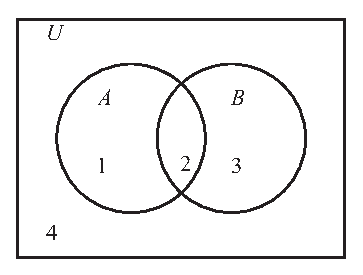
\includegraphics{figps-venn2.eps}
%\caption{Venn Diagram for Two Sets} \label{fig:venn2-prev}
\end{center}

\begin{enumerate}
  \item For the set $A^c$, regions 3 and 4 are shaded.
  \item For the set $B^c$, regions 1 and 4 are shaded.
  \item For the set $A^c \cup B$, regions 2, 3, and 4 are shaded.
  \item For the set $A^c \cup B^c$, regions 1, 3, and 4 are shaded.
  \item For the set $(A \cap B)^c$, regions 1, 3, and 4 are shaded.
  \item For the set $(A \cup B) - (A \cap B)$, regions 1, and 3 are shaded.
\end{enumerate}
\hbreak


\newpage

\endinput

\section*{Section~\ref{S:provingset} Proving Set Relationships}

\subsection*{Preview Activity 1 (Working with Two Specific Sets)}
\begin{enumerate} \setcounter{enumi}{1}
\item $S = \left\{ { \ldots ,  - 18,  - 12,  - 6, 0, 6, 12, 18,  \ldots } \right\}$ \quad
	$T = \left\{ { \ldots ,  - 6,  - 4,  - 2, 0, 2, 4, 6,  \ldots } \right\}$

It appears that  $S$  is a subset  of  $T$.

\item $S = \left\{ {x \in \mathbb{Z}\left. \right| x\text{ is a multiple of  6}} \right\}$ \quad
	$T = \left\{ {x \in \mathbb{Z}\left. \right| x\text{ is even}} \right\}$


\item An integer  $x$  is a multiple of  6  provided there exists an integer  $m$  such that  
$x = 6m$.

An integer  $y$  is an even integer provided there exists an integer  $k$  such that  
$y = 2k$.

\item Following is the completed know-show table.
\begin{table}[h]
$$
\BeginTable
\def\C{\JustCenter}
\BeginFormat
|p(0.4in)|p(2in)|p(1.8in)|
\EndFormat
  \_
  | \textbf{Step}  |  \textbf{Know}  |  \textbf{Reason}  |    \\+02 \_
|  $P$     |  $S$  is the set of all integers that are multiples of 6.
$T$ is the set of all even integers.  |  Hypothesis | \\ \_1
|  $P1$    |  Let  $x \in S$.         | Choose an arbitrary element of  $S$.  | \\ \_1
|  $P2$    | $\left( {\exists m \in \mathbb{Z}} \right)\left( {x = 6m} \right)$ | Definition of ``multiple'' | \\ \_1
|  $P3$    |  $x = (2 \cdot 3 ) m$        |  $6 = 2 \cdot 3$ | \\ \_1
|  $P4$    |  $x = 2 (3m)$                |  Associative Law | \\ \_1
|  $P5$    |  $x$ is even.                |  Definition of an even integer since $3m$ is an integer. | \\ \_1
|  $Q2$    |  $x$   is an element of  $T$. |  $x$ is even | \\ \_1
|  $Q1$    |  $\left( \forall x \in \Z \right) \left[ \left( x \in S \right) \to \left( x \in T \right) \right]$ |  Step  $P1$  and Step $Q2$            | \\  \_1 
|  $Q$     |  $S \subseteq T$. |  Definition of ``subset''          | \\ \_
%|  \textbf{Step}  |  \textbf{Show}  |  \textbf{Reason}     | \\+20 \_
\EndTable
$$
%\caption{Know-show table for Preview Activity~\ref{PA:working2sets}}
%\label{table:preview42}%
\end{table}
\end{enumerate}
\hbreak


\newpage
\subsection*{Preview Activity 2 (Working with Venn Diagrams)}
\begin{enumerate} 
\item The region in the Venn diagram on the left in Figure~1 corresponding to  $B^c $  is the region inside the rectangle that is outside the circle for  $B$.  This appears to be contained in the shaded region for  $A^c $.  Thus, it would appear that  $B^c  \subseteq A^c $.
%\addtocounter{enumi}{1}
\item In the general Venn diagram shown above, both  $A - B$
  and  $A \cap B^c $ are represented by region 1.  This suggests that  $A - B$  equals  
$A \cap B^c $.
\end{enumerate}
\vspace{-108pt}
\begin{figure}[h]
\begin{center}
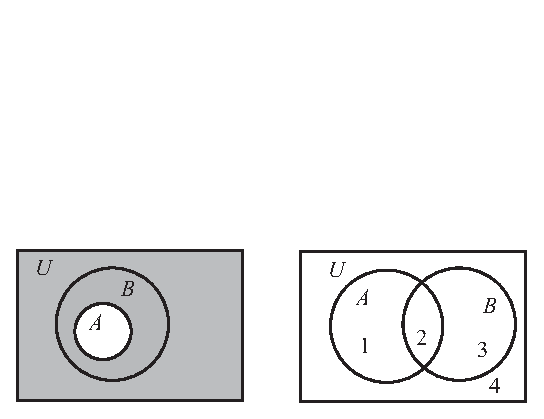
\includegraphics{figps-prev52.eps}
%\caption{Venn Diagrams for Preview Activity 2} \notag
\end{center}
\end{figure}

\hbreak

\newpage

\endinput

\section*{Section~\ref{S:setproperties} Properties of Set Operations}

\subsection*{Preview Activity 1 (Exploring a Relationship Between Two Sets)}
\begin{center}
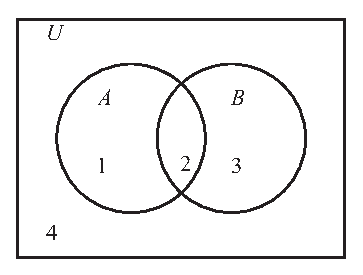
\includegraphics{figps-venn2.eps}
%\caption{Venn Diagram for Two Sets} \label{fig:venn2-prev}
\end{center}

\begin{enumerate}
\item In the standard Venn diagram for two sets, both  $\left( {A \cup B} \right)^c $  and  
$A^c  \cap B^c $ are represented by Region 4.	

\item Based on the Venn diagram, it appears that $\left( {A \cup B} \right)^c  = A^c  \cap B^c $.

\item An element  $x$  is not in $A \cup B$  means that  $x \notin A$  and  $x \notin B$.

\item An element  $x$  is in  $A^c $ means that  $x \notin A$.  In addition, $x \in B^c $  means that  
$x \notin B$.

\item An element  $x$  is in $A^c  \cap B^c $ means that   $x \in A^c $ and   $x \in B^c $.  So, $x \in A^c  \cap B^c $ means that   $x \notin A$ and   $x \notin B$.

\item The responses in (3) and (5) are equivalent.

\item As with the Venn diagram, this argument indicates that $\left( {A \cup B} \right)^c  = A^c  \cap B^c $.
\end{enumerate}
\hbreak



\subsection*{Preview Activity 2 (Proving that Statements Are Equivalent)}
\begin{enumerate}
\item 
\begin{tabular}[t]{| c | c | c || c | c | c | c | c | } \hline
$X$ & $Y$ & $Z$ &  $X \to Y$ & $Y \to Z$ & $X \to Z$ & $\left( {X \to Y} \right) \wedge \left( {Y \to Z} \right )$ & $\left[ {\left( {X \to Y} \right) \wedge \left( {Y \to Z} \right )} \right]$ \\ 
 & & & & & & & $\to \left( {X \to Z} \right)$ \\ \hline
T & T & T & T & T & T & T & T \\ \hline
T & T & F & T & F & F & F & T \\ \hline
T & F & T & F & T & T & F & T \\ \hline
T & F & F & F & T & F & F & T \\ \hline
F & T & T & T & T & T & T & T \\ \hline
F & T & F & T & F & T & F & T \\ \hline
F & F & T & T & T & T & T & T \\ \hline
F & F & F & T & T & T & T & T \\ \hline
\end{tabular}



\item The truth table in Part (1) shows that   
$\left[ {\left( {X \to Y} \right) \wedge \left( {Y \to Z} \right)} \right] \to \left( {X \to Z} \right)$  is a tautology.  (It is always true.)  This means that whenever we know that  $X \to Y$
  and that  $Y \to Z$, we can conclude that  $X \to Z$.

We are given that (1) $\left( {P \to Q} \right)$; (2) $\left( {Q \to R} \right)$; and  
(3) $\left( {R \to P} \right)$ are true.

\begin{enumerate}
\item So if the conditional statements in (1), (2), and (3) are true, then we know that  
$P \to Q$. We can use statements (2) and (3) to conclude that  $Q \to P$.  Therefore,  
$P \leftrightarrow Q$  is true.

\item We also know that  $Q \to R$, and we can use statements (3) and (1) to conclude that  
$R \to Q$.  Therefore,  $Q \leftrightarrow R$  is true.

\item We also know that  $R \to P$, and we can use statements (1) and (2) to conclude that  
$P \to R$.  Therefore,  $P \leftrightarrow R$  is true.
\end{enumerate}

\textbf{Note}:
When we have a list of three statements  $P$, $Q$,  and  $R$  such that  (1), (2), and (3) are true, we say that the three statements are \textbf{equivalent}.  This means that each of the statements in the list implies each of the other statements in the list.  

The purpose of this activity is to provide one way to prove that three (or more) statements are equivalent.  The basic idea is to prove a sequence of conditional statements (such as (1), (2), and (3)), so that there is an unbroken chain of conditional statements from each statement to every other statement.
\end{enumerate}
\hbreak

\newpage

\endinput

\section*{Section~\ref{S:cartesian} Cartesian Products}
\subsection*{Preview Activity 1 (An Equation with Two Variables)}
\begin{enumerate}
\item Each element of the truth set is an ordered pair such that when the first coordinate is substituted for  $x$  and the second coordinate is substituted for  $y$, the result is a true equation.  Following are some examples of ordered pairs that are in the truth set:  
$( {6, 0} )$, $( {0, 4} )$, $( {3, 2} )$, 
$( {12,  - 4} )$, $\left( {8, \dfrac{{ - 4}}{3}} \right)$, 
$\left( {\dfrac{{ - 3}}{2}, 5} \right)$, $\left( {\pi , \dfrac{{12 - 2\pi }}{3}} \right)$.

\item The graph is a straight line that passes through the points $( 0, 6 )$ and 
$( 4, 0 )$.  The graph shows the points whose ordered pairs are solutions of the equation  $2x + 3y = 12$

\item $S = \left\{ {\left. {( {x, y} )\,} \right| 2x + 3y = 12} \right\}$
\end{enumerate}
\hbreak



\subsection*{Preview Activity 2 (The Cartesian Product of Two Sets)}
\begin{enumerate}
\item $A \times B = \left\{ {( {1, a} ), ( {1, b} ), ( {2, a} ), ( {2, b} ), ( {3, a} ), ( {3, b} )} \right\}$.

\item The ordered pair  $( {3, a} ) \in A \times B$  since  $3 \in A$  and  $a \in B$.

\item The ordered pair  $( {3, a} ) \notin A \times A$  since  $a \notin A$.

\item The ordered pair $( {3, 1} ) \in A \times A$  since  $3 \in A$  and  $1 \in A$.

\item $A \times A = \left\{ {( {1, 1} ), ( {1, 2} ), ( {1, 3} ), ( {2, 1} ), ( {2, 2} ), ( {2, 3} ), ( {3, 1} ), ( {3, 2} ), ( {3, 3} )} \right\}$

\item The ordered pair  $( {x, y} ) \notin C \times D$  provided that  
$x \notin C$ or $y \notin D$.
\end{enumerate}
\hbreak



\newpage

\endinput

\section*{Section~\ref{S:indexfamily} Indexed Families of Sets}


\subsection*{Preview Activity 1 (The Union and Intersection of a Family of Sets)}

\begin{enumerate}
\item \begin{multicols}{2}
$A \cup B \cup C = \left\{1, 2, 3, 4, 5, 6, 7 \right\}$ \\
$B \cup C \cup D = \left\{2, 3, 4, 5, 6, 7, 8 \right\}$ \\
$A \cap B \cap C = \left\{3, 4, 5 \right\}$ \\
$B \cap C \cap D = \left\{4, 5, 6 \right\}$ 
\end{multicols}

\item 
\begin{enumerate}
\item $( A \cup B \cup C  ) \cup D = \left\{1, 2, 3, 4, 5, 6, 7, 8 \right\}$
\item $A \cup ( B \cup C  \cup D ) = \left\{1, 2, 3, 4, 5, 6, 7, 8 \right\}$
\item $A \cup ( B \cup C )   \cup D = \left\{1, 2, 3, 4, 5, 6, 7, 8 \right\}$
\item $( A \cup B ) \cup ( C \cup D ) = \left\{1, 2, 3, 4, 5, 6, 7, 8 \right\}$
\item $( A \cap B \cap C  ) \cap D = \left\{4, 5 \right\}$
\item $A \cap ( B \cap C  \cap D ) = \left\{4, 5 \right\}$
\item $A \cap ( B \cap C )   \cap D = \left\{4, 5 \right\}$
\item $( A \cap B ) \cap ( C \cap D ) = \left\{4, 5 \right\}$
\end{enumerate}

\item It appears that the placement of the parentheses in the union or intersection of these four sets does not make a difference.  This means that we can define $A \cup B \cup C \cup D$ and $A \cap B \cap C \cap D$ as $( A \cup B \cup C  ) \cup D$ and 
$( A \cap B \cap C  ) \cap D$, respectively.

\item Since $\mathscr{A} = \left\{A, B, C , D \right\}$,
\begin{itemize}
\item $\bigcup\limits_{X \in \mathscr{A}}^{}X$ consists of all the elements that are in one of the four sets $A$, $B$, $C$, and $D$.  This is the same set as  $A \cup B \cup C \cup D$.

\item $\bigcap\limits_{X \in \mathscr{A}}^{}X$ consists of all the elements that are in all of the four sets $A$, $B$, $C$, and $D$.  This is the same set as  $A \cap B \cap C \cap D$.
\end{itemize}  
So,
\[
\bigcup_{X \in \mathscr{A}}^{}X = \left\{1, 2, 3, 4, 5, 6, 7, 8 \right\} \qquad \text{and} \qquad
\bigcap_{X \in \mathscr{A}}^{}X = \left\{4, 5 \right\}.
\]

\item $\bigcup\limits_{X \in \mathscr{B}}^{}X = \left\{1, 2, 3, 4, 5, 6, 7, 8, 9, 10 \right\}$ \qquad and \qquad $\bigcap_{X \in \mathscr{B}}^{}X = \emptyset$

\item Recall the the universal set is $\N$.  Therefore,
\[
\left( \bigcup_{X \in \mathscr{A}}^{}X \right)^c = \left\{9, 10, 11, 12, 13, \ldots \right\}.
\]
In addition,
\begin{multicols}{2}
$A^c = \left\{6, 7, 8, 9, \ldots \right\}$ \\
$B^c = \left\{7, 8, 9, 10, \ldots \right\}$ \\
$C^c = \left\{8, 9, 10, 11, \ldots \right\}$ \\
$D^c = \left\{9, 10, 11, 12, \ldots \right\}$. 
\end{multicols}
Therefore,
\[
\bigcap_{X \in \mathscr{A}}^{}X^c = \left\{9, 10, 11, 12, \ldots \right\}.
\]
\end{enumerate}
\hbreak



\subsection*{Preview Activity 2 (An Indexed Family of Sets)}
\begin{enumerate}
\item $\bigcup\limits_{j=1}^{4}C_j = \left\{ 1, 2, 3, 4, 5, 6, 7, 8 \right\}$ \qquad and  \qquad
$\bigcap\limits_{j=1}^{4}C_j = \left\{ 4, 5 \right\}$

\item \begin{enumerate}
\item $\bigcup\limits_{j=1}^{6}C_j = \left\{ 1, 2, 3, 4, 5, 6, 7, 8, 9, 10 \right\}$ and  
$\bigcap\limits_{j=1}^{6}C_j = \emptyset$

\item $\bigcup\limits_{j=1}^{8}C_j = \left\{ 1, 2, 3, 4, 5, 6, 7, 8, 9, 10, 11, 12 \right\}$ and  $\bigcap\limits_{j=1}^{8}C_j = \emptyset$

\item $\bigcup\limits_{j=4}^{8}C_j = \left\{ 4, 5, 6, 7, 8, 9, 10, 11, 12 \right\}$ and  
$\bigcap\limits_{j=1}^{8}C_j = \left\{ 8 \right\}$


\item $( \bigcap\limits_{j=1}^{4}C_j )^c = \left\{1, 2, 3, 6, 7, 8, 9, 10, \ldots \right\}$ and \\
$\bigcup\limits_{j=1}^{4}C_j^c = \left\{1, 2, 3, 6, 7, 8, 9, 10, \ldots \right\}$

\end{enumerate}
\end{enumerate}
\hbreak



\newpage

\endinput


\section*{Section~\ref{S:introfunctions} Introduction to Functions}

\subsection*{Preview Activity 1 (Functions from Previous Courses)}

Equations (1), (3), (4), (6), and (7) can be used to define a function with  $x$  as the input and  $y$  as the output.  In Equation (7), the domain must be restricted to all real numbers not equal to 1.
\hbreak

\noindent
\subsection*{Preview Activity 2 (Some Other Types of Functions)}
\begin{enumerate}
\item \begin{enumerate}
\item The birthday function  $b$  is  a function since each person has exactly one birthday.

\item We can write the fact that Andrew Wiles'  birthday is April 11 as 
$b( {\text{Andrew Wiles}} ) = \text{ April 11}$.

\item The statement is true since there has been at least one person born on each day of the year.

\item The statement is false since there do exist different people who have the same birthday.
\end{enumerate}


\item \begin{enumerate}
%\item The domain of the function  $s$  is the set of natural numbers $\mathbb{N}$  .  We can also use   $\mathbb{N}$   as the codomain of   $s$.

\item \begin{multicols}{4}
$s( 1 ) = 1$	

$s( 2 ) = 3$	

$s( 3 ) = 4$	

$s( 4 ) = 7$

$s( 5 ) = 6$	

$s( 6 ) = 12$	

$s( 7 ) = 8$	

$s( 8 ) = 15$

$s( 9 ) = 13$	

$s( {10} ) = 18$	

$s( {11} ) = 12$	

$s( {12} ) = 28$

$s( {13} ) = 14$	

$s( {14} ) = 24$	

$s( 15 ) = 24$	

$s( {16} ) = 31$
\end{multicols}

%\item The numbers  $\sqrt 5$ , $\pi$ , and  $- 6$  are not natural numbers and hence, are not in the domain of the function  $s$. The domain of the function $s$ is the set of natural numbers $\N$.
%This means that  $s( {\sqrt 5 } )$, 
%$s( \pi  )$, and $s( { - 6} )$  are not defined.

\item There does not exist a natural number  $n$  such that  $s( n ) = 5$.  This can be seen by the values of  $s( 1 )$, $s( 2 )$, $s( 3 )$, and 
$s( 4 )$ in Part (2) and by observing that if  $n \geq 5$, then  1  and  $n$  are factors of  $n$, and so  $s( n ) > 5$.

\item Yes.  For example,  $s( 6 ) = s( {11} ) = 12$ and  
$s( {14} ) = s( {15} ) = 24$.

\item Part (b) shows that Statement (i) is false, and Part~(c) shows that Statement~(ii) is false.
\end{enumerate}
\end{enumerate}
\hbreak

\endinput

\section*{Section~\ref{S:moreaboutfunctions} More about Functions}

\subsection*{Preview Activity 1 (The Number of Diagonals of a Polygon)}
\begin{enumerate}
\item A triangle does not have any diagonals.  A square and a quadrilateral each have two diagonals.

\item \begin{multicols}{2}
\begin{tabular}[t]{| c | c | c | c | c |} \cline{1-2} \cline{4-5}
$n$ &  $d ( n )$ &  & $n$ & $d ( n )$   \\ \cline{1-2} \cline{4-5}
3  &  0  &  & 7  &  14  \\ \cline{1-2} \cline{4-5}
4  &  2  &  & 8  &  20  \\ \cline{1-2} \cline{4-5}
5  &  5  &  & 9  &  27  \\ \cline{1-2} \cline{4-5}
6  &  9  &  & 10 &  35  \\ \cline{1-2} \cline{4-5}
\end{tabular}

\item \begin{tabular}[t]{| c | c | c | c | c |} \cline{1-2} \cline{4-5}
  $x$ &  $f ( x )$ &  & $x$ & $f ( x )$   \\ \cline{1-2} \cline{4-5}
0  &  0  &  & 5  &  5  \\ \cline{1-2} \cline{4-5}
1  &  -1  &  & 6  &  9  \\ \cline{1-2} \cline{4-5}
2  &  -1  &  & 7  &  14  \\ \cline{1-2} \cline{4-5}
3  &  0  &  & 8  &  20  \\ \cline{1-2} \cline{4-5}
4  &  2  &  & 9  &  27  \\ \cline{1-2} \cline{4-5}
\end{tabular}
\end{multicols}

\item The outputs of the function  $f$  are determined  by a formula, and the outputs of the function  $d$  are determined by a verbal description. This does not mean the two functions are not equal.  However, the facts that the two functions have different domains and codomains would mean that these two functions are not equal.
\end{enumerate}
\hbreak



\subsection*{Preview Activity 2 (Derivatives)}
\begin{enumerate}
\item \begin{multicols}{2}
\begin{enumerate}
\item $f'( x ) = 4x^3  - 15x^2  + 3$
\item $g'( x ) =  - 5\sin ( {5x} )$
\item $h'( x ) = \dfrac{{x( {\cos x} ) - \sin x}}{{x^2 }}$
\item $k'( x ) =  - 2xe^{ - x^2 } $
\item $r'( x ) = \left\{ \begin{gathered}  1\text{     if  }x > 0 \hfill \\   - 1\text{  if  }x < 0 \hfill \\ \end{gathered}  \right.$
\end{enumerate}
\end{multicols}
Notice that the function  $r$  is not differentiable at $x=0$  .

\item Differentiation can be thought of as a function in the sense that if a function is considered the input, then the output is the derivative of that function.  The domain of the function is the set of all differentiable real functions and the codomain is the set of all real functions.
\end{enumerate}
\hbreak



\endinput


\endinput

%
%\include{xpart-activities}
%\newpage
%\thispagestyle{empty}
%$ $

%\include{xpart-exercises}
%
%\include{xpart-newsections}



% Set the ending of a LaTeX document
\end{document}
